% LaTeX source for textbook ``The Little Book of Semaphores, 2nd edition''
% Copyright 2016 Allen B. Downey.
% Copyright 1396 Persian version for github.com/ircsbooks

% Permission is granted to copy, distribute and/or modify this
% document under the terms of the Creative Commons
% Attribution-NonCommercial-ShareAlike 4.0 International (CC BY-NC-SA 4.0)
% http://creativecommons.org/licenses/by-nc-sa/4.0/

\documentclass{book}
\usepackage{fancyhdr}
\usepackage{listings}
\usepackage{graphicx}
\usepackage{color}
\usepackage{url}
\usepackage{makeidx}

\usepackage[colorlinks=true, linkcolor=blue, urlcolor=blue]{hyperref}


\usepackage[computeautoilg, extrafootnotefeatures]{xepersian}
\usepackage{bidiftnxtra}
\settextfont{IRXLotus}[Scale=1.2]%XB Niloofar}
\setdigitfont{Yas}
\setlatintextfont{Linux Libertine}[Scale=0.94]
%\defpersianfont\yasfont{Yas}
%\makeatletter
%    %کدهای زیر سبب نگارش تمامی‌ ارقام با قلم یاس می‌گردد. (در این قلم صفرها به صورت صحیح و توخالی نگاشته می‌شوند.)
%    \if@bidi@csundef{bidi@digits}{% 
%        \newcount\bidi@digits
%        \XeTeXinterchartokenstate=\@ne
%        \newXeTeXintercharclass\bidi@digits@charclass
%        \bidi@digits=`\0 \loop \XeTeXcharclass \bidi@digits \bidi@digits@charclass \ifnum\bidi@digits<`\9 \advance\bidi@digits \@ne \repeat
%        \bidi@digits=`\۰ \loop \XeTeXcharclass \bidi@digits \bidi@digits@charclass \ifnum\bidi@digits<`\۹ \advance\bidi@digits \@ne \repeat
%    }{}
%    \newif\if@q@verbatim
%    \bidi@appto\verbatim@font{\@q@verbatimtrue}
%    \bidi@appto\ttfamily{\@q@verbatimtrue}
%    \newXeTeXintercharclass\q@leftparen@charclass
%    \newXeTeXintercharclass\q@rightparen@charclass
%    \XeTeXcharclass `\( \q@leftparen@charclass
%    \XeTeXcharclass `\) \q@rightparen@charclass
%    \XeTeXcharclass `\[ \q@leftparen@charclass
%    \XeTeXcharclass `\] \q@rightparen@charclass
%    \XeTeXcharclass `\{ \q@leftparen@charclass
%    \XeTeXcharclass `\} \q@rightparen@charclass
%    \XeTeXcharclass `\« \q@leftparen@charclass
%    \XeTeXcharclass `\» \q@rightparen@charclass       
%    \XeTeXcharclass `\، \q@leftparen@charclass    
%    \XeTeXcharclass `\, \q@leftparen@charclass
%    \XeTeXcharclass `\؛ \q@leftparen@charclass          
%    \XeTeXcharclass `\; \q@leftparen@charclass          
%    \XeTeXcharclass `\: \q@leftparen@charclass          
%    \XeTeXcharclass `\. \q@leftparen@charclass     
%    \XeTeXcharclass `\- \q@leftparen@charclass     
%    \ifdim\the\XeTeXversion\XeTeXrevision\p@>0.99993\p@
%      \chardef\q@alloc@intercharclass@top=4095
%    \else
%      \chardef\q@alloc@intercharclass@top=255
%    \fi
%    \chardef\q@CharNormal=0
%    \XeTeXinterchartoks \q@alloc@intercharclass@top \bidi@digits@charclass = {\BeginSwitchDigitFont}
%    \XeTeXinterchartoks \bidi@digits@charclass \q@alloc@intercharclass@top = {\EndSwitchDigitFont}
%    \XeTeXinterchartoks \q@leftparen@charclass \bidi@digits@charclass = {\BeginSwitchDigitFont}
%    \XeTeXinterchartoks \bidi@digits@charclass \q@rightparen@charclass = {\EndSwitchDigitFont}
%    \XeTeXinterchartoks \q@rightparen@charclass \bidi@digits@charclass = {\BeginSwitchDigitFont}
%    \XeTeXinterchartoks \bidi@digits@charclass \q@leftparen@charclass = {\EndSwitchDigitFont}    
%    \XeTeXinterchartoks \q@CharNormal \bidi@digits@charclass = {\BeginSwitchDigitFont}
%    \XeTeXinterchartoks \bidi@digits@charclass \q@CharNormal = {\EndSwitchDigitFont}    
%    \if@bidi@csundef{if@nonlatin}{%
%        \newcommand*{\BeginSwitchDigitFont}{\if@q@verbatim\else%
%        \global\edef\currentfont{\the\font}\if@Latin\else\bgroup\yasfont \fi\fi}
%        \newcommand*{\EndSwitchDigitFont}{\if@q@verbatim\else\if@Latin\else\egroup\currentfont \fi\fi}
%    }{%
%        \newcommand*{\BeginSwitchDigitFont}{\if@q@verbatim\else%
%        \global\edef\currentfont{\the\font}\if@nonlatin\bgroup\yasfont \fi\fi}
%        \newcommand*{\EndSwitchDigitFont}{\if@q@verbatim\else\if@nonlatin\egroup\currentfont \fi\fi}
%    }    
%\makeatother


%\title{The Little Book of Semaphores}
\title{کتاب کوچک سمافورها}

%\author{Allen B. Downey}
\author{آلن بی.دونی\\[2cm]
%\vspace{2cm}
مترجمین:\\
سیّدمحمّدجواد رضویان، سیّدعلی آل‌طه و محمّدمهدی قاسمی‌نیا}

\newcommand{\theversion}{نسخه $2.2.1$}

\sloppy

\newcommand{\clearemptydoublepage}{\newpage\cleardoublepage}
\newcommand{\blankpage}{\newpage}

\pagestyle{fancyplain}

\renewcommand{\chaptermark}[1]{\markboth{#1}{}}
\renewcommand{\sectionmark}[1]{\markright{\thesection\ #1}{}}

\lhead[\fancyplain{}{\bfseries\thepage}]%
      {\fancyplain{}{\bfseries\rightmark}}
\rhead[\fancyplain{}{\bfseries\leftmark}]%
      {\fancyplain{}{\bfseries\thepage}}
\cfoot{}

% Commands that control the appearance of the listings
\definecolor{light-gray}{gray}{0.95}

\lstset{basicstyle=\tt, frame=single, 
backgroundcolor=\color{light-gray}, escapeinside={(*}{*)},
numbers=left, numberstyle=\tiny, numbersep=10pt}

\makeindex

\begin{document}
%\title {The Little Book of Semaphores}
%\author {Allen B. Downey}

\date {\theversion}
\maketitle

\vspace{2in}
\begin{center}
%{\Large The Little Book of Semaphores}
{\Large کتاب کوچک سمافورها}

%Second Edition
ویرایش دوم
\vspace{0.25in}

\theversion
\vspace{0.25in}

%Copyright 2016 Allen B. Downey
حق نشر $2016$ آلن بی.دونی
\end{center}
\vspace{0.25in}

%Permission is granted to copy, distribute and/or modify this
%document under the terms of the Creative Commons
%Attribution-NonCommercial-ShareAlike 4.0 International (CC BY-NC-SA 4.0)
%at \url{http://creativecommons.org/licenses/by-nc-sa/4.0}.
کپی، توزیع و/یا تغییر این سند تحت لایسنس زیر مجاز است: \\
\leftline{\lr{Creative Commons Attribution-NonCommercial-ShareAlike 4.0 International}}
\leftline{\lr{ (CC BY-NC-SA 4.0) \url{http://creativecommons.org/licenses/by-nc-sa/4.0}}}
%The original form of this book is LaTeX source code.
%Compiling this LaTeX source has the effect of generating
%a device-independent representation of a book, which
%can be converted to other formats and printed.
فرم اصلی این کتاب یک سورس کد لاتک است. کامپایل این سورس لاتک سبب تولید یک نمایش کتاب بدون وابستگی به دستگاه خواهد شد 
که می‌تواند به دیگر فرمت‌ها تبدیل و چاپ گردد. 

%This book was typeset by the author using latex, dvips and ps2pdf,
%among other free, open-source programs.
%The LaTeX source for this book is available from
%\url{http://greenteapress.com/semaphores}.
این کتاب توسط نویسنده با کمک لاتک، \lr{dvips} و \lr{ps2pdf} که همگی برنامه‌های کدباز هستند تایپ شده است. 
سورس لاتک این کتاب در آدرس \url{http://greenteapress.com/semaphores} موجود است.\footnote{در ترجمه این کتاب از زی‌لاتک و بسته 
زی‌پرشین استفاده شده است.}


\frontmatter

\chapter{پیشگفتار}

غالب کتاب‌های درسی سیستم‌های عامل در دوره کارشناسی بخشی در همگام سازی دارند که به طور معمول شامل معرفی اجزای اولیه‌ای (موتکس، سمافور، ناظر و متغیر‌های شرطی) و مسائل کلاسیک مثل خواننده نویسنده و تولیدکننده مصرف کننده.
وقتی که من در برکلی کلاسی سیستم‌عامل را داشتم، و در کالج کالبی این درس را تدریس کردم، به این نتیجه رسیدم که بیشتر دانشجویان قادر به درک راه حل ارائه شده برای اینگونه مسائل هستند، اما تنها برخی از این دانشجویان توانایی [ارئه چنین راه حل‌هایی][ارئه همان راه حل‌ها] و  حل مسائل مشابه را دارند.

یکی از دلایلی که دانشجویان نمی توانند به طور عمیق این قبیل مسایل را بفهمند، این است که وقت و تلاش بیشتری می برند از آنچیزی که کلاس‌ها در اختیارشان می گذارد.همگام‌سازی یکی از ماژول‌هایی است که نسبت به دیگر ماژول‌ها وقت بیشتری نیاز دارد. و من مطمئن نیستم که بتوانم برای این منظور دلایلی را شرح دهم، منتها من فکر می کنم که سمافور‌ها یکی از چالشی‌ترین، جالب‌ترین و سرگرمی‌ترین بخش‌های سیستم‌عامل می باشد.
با هدف شناساندن  اصطلاحات والگوهای همگام‌سازی به گونه ای که به صورت مستقل قابل درک باشد و بتوان از آنها برای حل مسائل پیچیده استفاده نمود، اولین ویرایش این کتاب نوشتم.
نوشتن کدهمگام‌سازی چالش‌های مختص به خود را دارد زیرا که با افزایش تعداد اجزا و تعداد تعاملات به طور غیر قابل کنترلی افزایش می یابد.


با این وجود در بین راه حل هایی که دیدم، الگوهایی یافتم و حداقل برخی  ره‌یافت‌های روشمند درست برای ترکیب راه حل‌ها رسیدم.
شانسی این را داشتم که در زمانی که در کالج ویلسلی بودم، این کتاب را به همراه کتاب درسی استاندارد استفاده کردم و در زمان تدریس درس مبحث همگام سازی را به شکل موازی با درس تدریس می کردم. هر هفته به دانشجویان چند صفحه از کتاب را می دادم که با یک معما تمام می شد و گاهی اوقات یه راهنمایی مختصر. و به آنها توصیه می کردم که به راهنمایی نگاه نکننده مگر اینکه گیر افتاده باشند.
و همچنین ابزارهایی برای تست راه حل‌ها دادم، یه تخته مغناطیسی کوچک که می تونستن کدهاشون رو بنویسند و یک بسته آهنربا برای نمایش تردهای در حال اجرا.

نتیجه بسیار چشمگیر بود، هر چه زمان بیشتری در اختیار داشنجویان می گذاشتم، عمق فهمشون بیشتر می شد، مهمتر اینکه غالبشون قادر به حل بیشتر معماها بودند، و در برخی حالات همان راه حل‌های کلاسیک را می یافتند و یا راه حل جدیدی را ایجاد می کردند.
وقتی که رفتم کالج گام بعدی را با ایجاد کلاس فوق‌برنامه همگام سازی برداشتم، که در آن کلاس این کتاب تدریس می شد و همچنین پیاده سازی دستورات اولیه همگام‌سازی در زبان اسمبلی \lr{x86} و پاسیکس و پیتون.
دانشجویانی که این درس را گرفتند در یافتن خطاهای نسخه نخست کمک کردند و چندتا از آنها راه حل‌هایی بهتر از راه حل‌های من ارائه داند در پایان ترم از هر کدام انها خواستم که یک مسائله جدید با ترجیحا با یک راه حل بنویسند. از این مشارکت‌ها در نسخه دوم استفاده کردم.

بخش باقی مانده از پیشگفتار:
همچنین، پس از عرضه ی ویرایش اول، کنث ریک (Kenneth Reek) مقاله ی «الگوهای طراحی سمافورها» را در «گروه ویژه ی علاقمند به آموزش علوم کامپیوتر در ACM» ارائه داد. او در این مقاله مسأله ای را که من به آن «مسئله ی سوشی بار» می گویم معرفی و دو راه حل برای اثبات الگوهایی که وی آن‌ها را «دست به دست کردن باتوم» و «این کار را برای تو می کنم» نامید مطرح کرد. هنگامی که با این الگوها آشنا شدم، توانستم آن‌ها را در مسائل ویرایش اول کتاب به کار برم و راه حل هایی تولید کنم که به نظرم بهتر هستند.
تغییر دیگر در نسخه دوم، نوع نگارش یا نحو آن است. بعد از آنی که نسخه اول را نوشتم، من زبان برنامه نویسی پی‌تون را که نتنها یکی از عالیترین زبان‌های برنامه نویسی است بلکه یک زبان بسیار شبیه به شبه‌کد است را یاد گرفتم. در نتیجه من از یک شبه کد شبیه به c در ویرایش نخست به یک شبه کد شبیه به زبان پی‌تون تغیر دادم. در حقیقت، من یک شبیه ساز نوشتم که بسیاری از راه حل‌های ارائه شده در این کتاب را می تواند اجرا کند. خواننده هایی هم که با زبان پی‌تون آشنا نیستند نیز (ان‌شالله) می توانند آن را درک کنند.در مواردی که از ویژگی‌های زبان پی‌تون استفاده کردم، نحو زبان پی‌تون و نحوه‌ی کار کد را شرح داده‌ام. امیدوارم این تغیر زمینه خوانا تر کردن کتاب را بوجود آورده باشد. صفحه بندی این کتاب ممکن است کمی عجیب به نظر برسد! اما صفحات خالی نیز خود یک روش سودمند است، بعد از هر معما، یک فضای خالی را تا شبه‌راهنمایی که در صفحه بعد است، گذاشته ام و بعد از آن یک صفحه خالی دیگر برای حل مساله تا صفحه نمایش راه حل نهایی. زمانی که من از این کتاب در کلاسم استفاده می کنم، برخی از صفحات را از کتاب جدا می کنم و دانشجواینم آنها را بعدا صحافی می کنند! این سیستم صفحه بندی امکان جداکردن معما را بدون صفحات مربوط به راهنمایی ها، محقق می‌کند. بعضی اوقات بخش مربوط به راهنمایی را تا می کنم و از دیده شدن آن جلوگیری می کنم تا دانشجویان خود به حل مساله پرداخته و در زمان مناسب راه حل را ببینند. اگر کتاب را به شکل تک صفحه چاپ کنید(به شکل یک رو سفید! زمانی که پولتان زیادی کرده باشد!مترجم) می توانید از چاپ صفحه‌های سفید خودداری کنید(ظاهرا نویسنده برای ایالت‌های اصفهان نشین آمریکا هستند!مترجم). 
این کتاب یک کتاب رایگان است، این بدین معنی است که هر شخصی می تواند آنرا بخواند، رونوشت برداری کند، اصلاح کند و حتی بازپخش کند و اینها به دلیل نوع لیسانس مورد استفاده برای این کتاب است.امیدوارم افراد این کتاب را مناسب و کارا ببینند، اما بیشتر از آن امیدوارم که آنها برای ادامه فرایند توسعه ایرادات و پیشنهادات خود و همینطور مطالب بیشتر خود را برایم ارسال کنند.
با تشکر
\vspace{0.3in}
\noindent آلن دونی \\
\noindent نیدهام، ماساچوست \\
\noindent سه شنبه، ۱۲ خرداد ۱۳۸۳\\


%\section*{Contributor's list}
\section*{لیست همکاران}

%The following are some of the people who have contributed to this
%book:
در ادامه لیست برخی افرادی که در این کتاب مشارکت داشته‌اند آمده است:

\begin{itemize}

%\item Many of the problems in this book are variations of classical
%problems that appeared first in technical articles and then in textbooks.
%Whenever I know the origin of a problem or solution, I acknowledge it
%in the text.
\item    
    بسیاری از مسائل این کتاب گونه‌ٔ دیگری از مسائل کلاسیکی است که ابتدا در مقالات تخصصی آمده‌اند و سپس در کتب مرجع. 
    هر کجا که منبع یک مسأله یا راه حل را بدانم در متن به آن اشاره خواهم داشت. 

%\item I also thank the students at Wellesley College who worked with
%the first edition of the book, and the students at Olin College who
%worked with the second edition.
\item 
    همچنین از دانشجویان \lr{Wellesley College} که با ویرایش اول این کتاب کار کرده‌اند تشکر می‌نمایم و نیز دانشجویان 
    \lr{Olin College} 
    که با ویرایش دوم کتاب سر و کار داشتند. 

%\item Se Won sent in a small but important correction in my presentation
%of Tanenbaum's solution to the Dining Philosophers Problem.
\item 
    \lr{Se Won} 
    تصحیح کوچکی --لکن مهم-- را در ارائه راه حل \lr{Tanenbaum} نسب به مسالهٔ فیلسوف‌های در حال غذا خوردن ارسال نموده است. 

%\item Daniel Zingaro punched a hole in the Dancer's problem, which
%provoked me to rewrite that section.  I can only hope that it makes more
%sense now.  Daniel also pointed out an error in a previous version of
%my solution to the H$_2$O problem, and then wrote back a year later
%with some typos.
\item \lr{Daniel Zingaro}
    در مسالهٔ \lr{Dancer} نکته‌ای را متذکر گردید که سبب بازنویسی مجدد آن بخش گردید. امیدوارم اکنون با معنی‌تر شده باشد. 
    علاوه بر این \lr{Daniel} یک خطا را در نسخهٔ قبلی راه حل مساله \lr{H$_2$O} نشان داده است و سال بعد از آن نیز 
    تعدادی خطاهای تایپی را متذکر شده است. 
    
    


%\item Thomas Hansen found a typo in the Cigarette smokers problem.
\item \lr{Thomas Hansen}
    یک خطای تایپی را در مساله \lr{Cigarette smokers} یافته است. 


%\item Pascal R\"{u}tten pointed out several typos, including my embarrassing
%misspelling of Edsger Dijkstra.
\item \lr{Pascal R\"{u}tten}
    به چندین اشکال تایپی اشاره نموده است از جمله تلفظ نادرست \lr{Edsger Dijkstra}.

%\item Marcelo Johann pointed out an error in my solution to the
%Dining Savages problem, and fixed it!
\item \lr{Marcelo Johann}
    خطایی را در راه حل مسالهٔ \lr{Dining Savages} یافته و آن را اصلاح کرده است. 


%\item Roger Shipman sent a whole passel of corrections as well as
%an interesting variation on the Barrier problem.
\item \lr{Roger Shipman}
    تمام اصلاحات به علاوه یک گونهٔ جذاب از مساله \lr{Barrier} را ارسال نموده است. 
    
    

%\item Jon Cass pointed out an omission in the discussion of dining
%philosophers.
\item \lr{ Jon Cass} 
    یک از قلم افتادگی را در مساله فیلسوف‌های در حال غذا خوردن مشخص نموده است.
    

%\item Krzysztof Ko\'{s}ciuszkiewicz sent in several corrections, including
%a missing line in the Fifo class definition.
\item \lr{Krzysztof Ko\'{s}ciuszkiewicz}
    چندین اصلاح از جمله از قلم افتادن خطی در تعریف کلاس \lr{Fifo} را فرستاده است. 

%\item Fritz Vaandrager at the Radboud University Nijmegen in the
%Netherlands and his students Marc Schoolderman, Manuel Stampe and Lars
%Lockefeer used a tool called UPPAAL to check several of the solutions
%in this book and found errors in my solutions to the Room Party problem
%and the Modus Hall problem.
\item \lr{Fritz Vaandrager}
    از دانشگاه \lr{Radboud} هلند و دانشجویانش 
    \lr{Marc Schoolderman}، \lr{Manuel Stampe} و \lr{Lars Lockefeer}
    ابزاری بنام \lr{UPPAAL} را به منظور بررسی چندین راه حل این کتاب بکار برده و خطاهایی را در راه حل‌های ارائه شده برای 
    مساله‌های \lr{Room Party} و \lr{Modus Hall}  یافته‌اند. 
    


%\item Eric Gorr pointed out an explanation in Chapter 3 that was
%not exactly right.
\item \lr{Eric Gorr }
    درست نبودن یک توضیح در فصل سوم را مشخص نموده است. 


%\item Jouni Lepp\"{a}j\"{a}rvi helped clarify the origins of semaphores.
\item  \lr{ Jouni Lepp\"{a}j\"{a}rvi} 
    در واضح نمودن مبدأ سمافورها کمک نموده است. 

%\item Christoph Bartoschek found an error in a solution to
%the exclusive dance problem.
\item \lr{Christoph Bartoschek} 
    خطایی در راه حل مساله رقص انحصاری را یافته است. 

%\item Eus found a typo in Chapter 3.
\item \lr{Eus} یک خطای تایپی در فصل سوم را پیدا کرده است. 

%\item Tak-Shing Chan found an out-of-bounds error in {\tt counter\_mutex.c}.
\item \lr{Tak-Shing Chan} 
    یک خطای خارج از محدوده\LTRfootnote{out-of-bounds} را در \lr{{\tt counter\_mutex.c}} یافته است. 

%\item Roman V. Kiseliov made several suggestions for improving
%the appearance of the book, and helped me with some \LaTeX~issues.
\item \lr{Roman V. Kiseliov}
    چند پیشنهاد برای بهبود ظاهر کتاب ارائه داده و با چند نکته در \lr{\LaTeX} مرا راهنمایی نموده است. 
    
%\item Alejandro C\'{e}spedes is working on the Spanish translation of this
%book and found some typos.
\item   \lr{Alejandro C\'{e}spedes} 
    در حال کار روی ترجمه اسپانیایی این کتاب است و چندین غلط تایپی را در آن یافته است. 

%\item Erich Nahum found a problem in my adaptation of Kenneth Reek's
%  solution to the Sushi Bar Problem.
\item \lr{Erich Nahum} 
    مشکلی را در تطبیق راه حل \lr{Kenneth Reek} نسبت به مساله \lr{Sushi Bar} یافته است. 

%\item Martin Storsj\"{o} sent a correction to the generalized smokers problem.
\item \lr{Martin Storsj\"{o}}
    تصحیحی در مساله \lr{generalized smokers} را ارسال نموده است. 
    
%\item Cris Hawkins pointed out an unused variable.
\item \lr{Cris Hawkins}
    به یک متغیر بدون استفاده اشاره نموده است. 

%\item Adolfo Di Mare found the missing ``and''.
\item \lr{Adolfo Di Mare }
    یک \lr{``and''} از جا افتاده را یافته است. 

%\item Simon Ellis found a typo.
\item \lr{Simon Ellis} یک خطای تایپی را یافته است. 

%\item Benjamin Nash found a typo, an error in one solution, and
%a malfeature in another.
\item \lr{Benjamin Nash}    یک خطای تایپی و خطایی در یک راه حل و مشکل دیگری را یافته است. 

%\item Alejandro Pulver found a problem with the Barbershop solution.
\item \lr{Alejandro Pulver} 
    مشکلی را در راه حل مساله \lr{Barbershop}  یافته است. 

\end{itemize}

% endcontrib

\tableofcontents
\clearemptydoublepage

\mainmatter


\chapter{معرفی}

\section{به‌هنگام سازی}
\label{synch}

اصطلاحا همگام‌سازی به معنی وقوع همزمان دو چیز است. در سسیتم‌های کامپیوتری همگام‌سازی کلی‌تر است. این به معنی رابطه مابین رویدادهاست، در هر تعداد از رویدادها و هر نوع رابطه(قبل، حین، بعد).
غالبا برنامه‌نویسان با محدودی‌ت‌های همگام‌سازی مواجه‌اند، که این محدودیت‌ها الزاماتی در ارتباط با ترتیب این رخدادها می باشد.

\begin{description}

\item[تسلسل:] رخداد الف پیش از رخداد ب اتفاق می افتد.

\item[انحصار متقابل:] رخداد الف و ب نباید در یک زمان رخ دهد.

\end{description}
در زندگی واقعی عالبت محدودیت‌های همگامی سازی را با کمک یک ساعت بررسی و اعمال می کنیم. چگونه می فهمیم که رخداد الف قبل از رخداد ب رخ داده است؟ با دانستن زمان رخداد هر دو واقعه را بدانیم، می توانیم زمان‌ها را با هم مقایسه کنیم.
در سیستم‌های کامپیوتری غالبا نمی توانیم از ساعت در محدودیت‌های همگام سازی‌های کامپیوتری را برآورده کنیم، زیر را که هیچ ساعت جهانی به دلیل اینکه زمان دقیق وقوع رویدادها را نمی دانیم.
این کتاب درباره تکنیکهای نرم افزار برای اعمال‌های مجدودیت‌های همگام‌سازی در کامپیوتر است.



%\section {Execution model}
\section {مدل اجرایی}

%In order to understand software synchronization, you have to
%have a model of how computer programs run.  In the simplest
%model, computers execute one instruction after another in
%sequence.  In this model, synchronization is trivial; we can
%tell the order of events by looking at the program.  If Statement
%A comes before Statement B, it will be executed first.

    به منظور درک همگام‌سازی نرم‌افزاری، باید مدلی از چگونگی اجرای برنامه‌های کامپیوتری داشته باشید.
    در ساده‌ترین مدل، کامپیوترها دستورات را به ترتیب یکی پس از دیگری اجرا می‌نمایند. 
    در این مدل، همگام‌سازی بدیهی است؛‌ ترتیب وقایع را با نگاه به  برنامه می‌توان بیان نمود. 
    اگر دستور \lr{A} قبل از دستور \lr{B} آمده باشد، اوّل اجرا می‌گردد. 

%There are two ways things get more complicated.  One possibility
%is that the computer is parallel, meaning that it has multiple
%processors running at the same time.  In that case it is not easy
%to know if a statement on one processor is executed before a
%statement on another.
%    دو طریق کار را پیچیده خواهد کرد. 
    در دو صورت همگام‌سازی پیچیده خواهد شد. 
    ممکن است کامپیوتر موازی باشد بدین معنی که چندین پردازنده در یک زمان در حال اجرا باشد. در این حالت نمی‌توان به سادگی فهمید که 
    دستوری در یک پردازنده قبل از دستور دیگری در پردازنده دیگر اجرا شده است. 

%Another possibility is that a single processor is running multiple
%threads of execution.  A thread is a sequence of instructions
%that execute sequentially.  If there are multiple threads, then
%the processor can work on one for a while, then switch to
%another, and so on.
    و یا ممکن است یک پردازنده چندین نخ اجرایی داشته باشد. نخ دنباله‌ای از دستورات است که به به ترتیب اجرا می‌شوند. 
    اگر چندین نخ وجود داشته باشد آنگاه پردازنده می‌تواند برای مدتی بر روی یکی  از نخ‌ها کار کند و سپس به نخی دیگر منتقل شود و به همین 
    ترتیب ادامه دهد. 

%In general the programmer has no control over when each thread runs;
%the operating system (specifically, the scheduler) makes those
%decisions.  As a result, again, the programmer can't tell when
%statements in different threads will be executed.
    به طور کلی برنامه‌نویس هیچ کنترلی روی اجرای نخ‌ها ندارد؛ در واقع سیستم‌عامل (بخصوص زمان‌بند) در این باره تصمیم‌ می‌گیرد. 
    در نتیجه برنامه‌نویس نمی‌تواند بگوید که دستورات چه زمانی در نخ‌های مختلف اجرا خواهد شد.
    
%For purposes of synchronization, there is no difference between the
%parallel model and the multithread model.  The issue is the
%same---within one processor (or one thread) we know the order of
%execution, but between processors (or threads) it is impossible to
%tell.

    در همگام‌سازی، تفاوتی بین مدل موازی و مدل چند نخی وجود ندارد. 
    مساله یکی است--در یک پردازنده (یا یک نخ) ترتیب اجرا مشخص است امّا بین پردازنده‌ها (یا نخ‌ها) بیان این ترتیب غیر ممکن است. 
    
%A real world example might make this clearer.  Imagine that you and
%your friend Bob live in different cities, and one day, around dinner
%time, you start to wonder who ate lunch first that day, you or Bob.
%How would you find out?
    یک مثال واقعی این مساله را روشن‌تر می‌نمایند. 
    تصور کنید که شما و دوستتان \lr{Bob} در شهرهای متفاوتی زندگی می‌کنید. یک روز نزدیک وقت ناهار، شما به این فکر می‌افتید که 
    چه کسی امروز زودتر ناهار خواهد خورد، شما یا \lr{Bob}. چگونه این را در می‌یابید؟ 
    

%Obviously you could call him and ask what time he ate lunch.  But what
%if you started lunch at 11:59 by your clock and Bob started lunch at
%12:01 by his clock?  Can you be sure who started first?  Unless you
%are both very careful to keep accurate clocks, you can't.
    به سادگی می‌توانید به او زنگ بزنید و بپرسید که چه زمانی ناهار خورده است. امّا اگر شما با ساعت خودتان در ۱۱/۵۹ غذا را شروع نموده باشید 
    و \lr{Bob} با ساعت خودش در ۱۲/۰۱، آن وقت چه؟ آیا می‌توانید مطمئن باشید که چه کسی زودتر شروع نموده است؟ 
    تنها در صورتی ممکن است که هر دوی شما نسبت به دقیق بودن ساعت‌هایتان حساس بوده باشید.

%Computer systems face the same problem because, even though their
%clocks are usually accurate, there is always a limit to their
%precision.  In addition, most of the time the computer does not keep
%track of what time things happen.  There are just too many things
%happening, too fast, to record the exact time of everything.

    سیستم‌های کامپیوتری با مشکل مشابهی مواجه هستند زیرا با وجود اینکه معمولاً ساعت‌هایشان دقیق است امّا همیشه 
    در میزان دقت ساعت‌ها محدودیت وجود دارد. به علاوه، در بیشتر وقت‌ها کامپیوتر زمان وقوع رخدادها را دنبال نمی‌نماید. 
    چرا که تعداد بسیار زیادی رخداد آن هم با سرعتی بسیار در حال وقوع است که ذخیره  زمان دقیق همه آن‌ها ممکن نیست. 
    
%Puzzle: Assuming that Bob is willing to follow simple instructions, is
%there any way you can {\em guarantee} that tomorrow you will eat lunch
%before Bob?
    معمّا: با فرض اینکه \lr{Bob} می‌خواهد دستورات ساده‌ای را دنبال نماید آیا راهی وجود دارد که تضمین نمایید فردا شما زودتر از او ناهار خواهید خورد؟
    
\clearemptydoublepage
%\section {Serialization with messages}
\section {تسلل به کمک پیام‌دهی}
\label{serialization}

%One solution is to instruct Bob not to eat lunch until you call.
%Then, make sure you don't call until after lunch.  This approach may
%seem trivial, but the underlying idea, message passing, is a real
%solution for many synchronization problems.
%At the risk of belaboring the obvious, consider this timeline.
    یک راه آن است که به \lr{Bob} بگویید تا شما به او زنگ نزده‌اید ناهار نخورد. شما نیز  اطمینان دهید پس از ناهار زنگ می‌زنید. 
    اگر چه این راهکار بدیهی به نظر می‌رسد لکن ایدهٔ پایهٔ آن، تبادل پیام\LTRfootnote{message passing}، راه حل واقعی برای بسیاری
    از مسائل همگام‌سازی می‌باشد.  جدول زمانی زیر را در نظر بگیرید. 
    
%
\begin{latin}
\begin{minipage}[t]{2in}
\begin{latin}
\begin{lstlisting}[title=\rl{نخ \lr{A} (شما)}]{}
Eat breakfast 
Work          
Eat lunch     
Call Bob
\end{lstlisting}
\end{latin}
\end{minipage}
\hfill
\begin{minipage}[t]{2in}
\begin{latin}
\begin{lstlisting}[title=\rl{نخ \lr{B} (‌Bob)}]{}
Eat breakfast
Wait for a call
Eat lunch
\end{lstlisting}
\end{latin}
\end{minipage}
\end{latin}
%
%The first column is a list of actions you perform; in other words,
%your thread of execution.  The second column is Bob's thread of
%execution.  Within a thread, we can always tell what order things
%happen.  We can denote the order of events
    اولین ستون لیست اعمالی است که شما انجام می‌دهید؛ به عبارت دیگر نخ اجرای شما. 
    ستون دوم نیز نخ اجرای \lr{Bob} است. درون یک نخ همیشه می‌توانیم ترتیب اجرای وقایع را بگوییم. 
    ترتیب وقایع را به این صورت می‌توانیم نشان دهیم
%
\begin{eqnarray*}
a1 < a2 < a3 < a4  \\
b1 < b2 < b3
\end{eqnarray*}
%
%where the relation $a1 < a2$ means that a1 happened before a2.
    که رابطه  $a1 < a2$ به معنای وقوع  $a1$ پیش از  $a2$ است. 

%In general, though, there is no way to compare events from different
%threads; for example, we have no idea who ate breakfast first (is $a1
%< b1$?).
    ولی در کل هیچ راهی برای مقایسه رخدادهای نخ‌های مختلف نداریم؛ برای مثال ایده‌ای از اینکه چه کسی ابتدا صبحانه می‌خورد نداریم 
    (آیا $a1 < b1$  است؟).
    
%But with message passing (the phone call) we {\em can} tell who ate
%lunch first ($a3 < b3$).  Assuming that Bob has no other friends, he
%won't get a call until you call, so $b2 > a4$ .  Combining all the
%relations, we get
    امّا با کمک تبادل پیام (تماس تلفنی) می‌توانیم بگوییم چه کسی زودتر ناهار خورده است ($a3 < b3$).
    با فرض اینکه باب هیچ دوست دیگری نداشته باشد هیچ تماسی جز از شما دریافت نخواهد کرد بنابراین  ($b2 > a4$).
    با ترکیب تمامی روابط، داریم 
%
\begin{eqnarray*}
b3 > b2 > a4 > a3
\end{eqnarray*}
%
%which proves that you had lunch before Bob.
    که ثابت می‌کند شما قبل از باب ناهار خورده‌اید. 

%In this case, we would say that you and Bob ate lunch
%{\bf sequentially}, because we know the order of events, and you
%ate breakfast {\bf concurrently}, because we don't.

    در این حالت، می‌گوییم شما و باب به صورت \textbf{متوالی}\LTRfootnote{sequential} ناهار خورده‌اید زیرا 
    ترتیب وقایع را می‌دانیم. از طرف دیگر صبحانه را به صورت  \textbf{همروند}\LTRfootnote{concurrent} خورده‌اید 
    زیرا که ترتیب مشخص نیست. 
    
%When we talk about concurrent events, it is tempting to say
%that they happen at the same time, or simultaneously.  As a
%shorthand, that's fine, as long as you remember the strict
%definition:
    مواقعی که درباره رخدادهای همروند صحبت می‌کنیم، اینکه بگوییم آن‌ها در یک زمان یا به صورت همزمان رخ می‌دهد بی‌راه نیست هر چند که دقیق هم نیست. 
%    مواقعی که در.... ، معمولاً منظورمان این است که آن‌ها با هم یا همزمان اتفاق افتاده‌اند که می‌تواند دقیق هم نباشد. 
    تعبیر فوق تا زمانی که تعریف دقیق زیر را در خاطر دارید بلامانع است:

\begin{quote}
%Two events are concurrent if we cannot tell by looking at
%the program which will happen first.
    دو واقعه، همروند هستند اگر با نگاه به برنامه نتوانیم بگوییم کدامیک زودتر رخ می‌دهد. 
\end{quote}

%Sometimes we can tell, after the program runs, which happened first,
%but often not, and even if we can, there is no guarantee that we will
%get the same result the next time.
    گاهی اوقات پس از اجرای برنامه می‌‌توانیم بگوییم که کدامیک ابتدا رخ داده است امّا غالباً ممکن نیست و حتی اگر هم بتوانیم 
    باز هم تضمینی نیست که مرتبه بعد نتیجه‌ای یکسان بگیریم. 
%%Sun 20 Aug 2017 06:48:49 PM +0430
\newpage
%\section {Non-determinism}
\section{عدم قطعیت}

%Concurrent programs are often {\bf non-deterministic}, which means it
%is not possible to tell, by looking at the program, what will happen
%when it executes.  Here is a simple example of a
%non-deterministic program:
    برنامه‌های همروند اغلب \textbf{غیر قطعی}\LTRfootnote{non-determinism} هستند به این معنی که با نگاه به برنامه 
    امکان اینکه بگوییم با اجرای آن چه چیزی رخ خواهد داد، وجود ندارد. در ادامه یک برنامه سادهٔ غیر قطعی آمده است:

\begin{latin}
\begin{minipage}[t]{2in}
\begin{latin}
\begin{lstlisting}[title=\rl{نخ \lr{A}}]{}
print "yes"
\end{lstlisting}
\end{latin}
\end{minipage}
\hfill
\begin{minipage}[t]{2in}
\begin{latin}
\begin{lstlisting}[title=\rl{نخ \lr{‌B}}]{}
print "no"
\end{lstlisting}
\end{latin}
\end{minipage}
\end{latin}

%Because the two threads run concurrently, the order of
%execution depends on the scheduler.  During any given run
%of this program, the output might be ``yes no'' or ``no yes''.
    از آنجایی که دو نخ به صورت همروند اجرا می‌شوند، ترتیب اجرا بستگی به زمان‌بند دارد. در هر اجرای این برنامه، خروجی ممکن است 
    \lr{`yes no''}  یا \lr{``no yes''}
     باشد. 
     
%Non-determinism is one of the things that makes concurrent
%programs hard to debug.  A program might work correctly
%1000 times in a row, and then crash on the 1001st run, depending
%on the particular decisions of the scheduler.
    عدم قطعیت یکی از مواردی است که اشکال‌زدایی برنامه‌های همروند را مشکل می‌سازد. برنامه‌ای ممکن است $1000$ بار بر روی یک سطر به درستی 
    کار کرده و سپس در اجرای $1001$ام بسته به تصمیمات خاص زمان‌بند با مشکل مواجه شده و اجرای برنامه متوقف شود. 
    
%These kinds of bugs are almost impossible to find by testing;
%they can only be avoided by careful programming.
    تقریبا پیدا کردن این نوع خطاها با بررسی کد ناممکن است؛  این نوع  خطاها تنها از طریق دقت در برنامه‌نویسی قابل اجتناب هستند. 


%\section {Shared variables}
\section {متغیرهای اشتراکی}
\label{shared}

%Most of the time, most variables in most threads are {\bf local},
%meaning that they belong to a single thread and no other threads
%can access them.  As long as that's true, there tend to be few
%synchronization problems, because threads just don't interact.
    بیشتر مواقع، غالب متغیرها در اکثر نخ‌ها \textbf{محلی}\LTRfootnote{local} هستند، بدین معنی که تنها به یک نخ تعلق دارند و 
    سایر نخ‌ها نمی‌توانند به آن‌ها دسترسی داشته باشند. تا زمانیکه این نکته برقرار است، مشکلات همگام‌سازی کمی وجود خواهد داشت زیرا که 
    نخ‌ها دخالتی در آن متغیرها ندارند. 

%But usually some variables are {\bf shared} among two or more
%threads; this is one of the ways threads interact with each other.
%For example, one way to communicate information between threads is
%for one thread to read a value written by another thread.
    امّا گاهی اوقات برخی متغیرها بین دو یا چند نخ به صورت \textbf{اشتراکی}\LTRfootnote{shared} هستند؛ این 
    یکی از شیوه‌های تعامل نخ‌ها با یکدیگر است. برای مثال، یک راهِ  تبادل اطلاعات بین نخ‌ها، این است که نخی مقداری را بخواند و نخ دیگر آن را بنویسد. 
    
%If the threads are unsynchronized, then we cannot tell by looking at
%the program whether the reader will see the value the writer writes
%or an old value that was already there.
%Thus many applications enforce the constraint that the reader
%should not read until after the writer writes.  This is exactly
%the serialization problem in Section~\ref{serialization}.
    اگر نخ‌ها ناهمگام باشند آنگاه با نگاه کردن به کد نمی‌توانیم بگوییم که آیا نخ خواننده مقداری را که نویسنده نوشته است می‌بیند یا همان مقدار قبلی را خواهد دید. 
    لذا بسیاری از برنامه‌ها محدودیت‌هایی را بر روی خواننده‌ها اعمال می‌نمایند تا زمانیکه نویسنده مقدار را ننوشته است چیزی را نخواند. 
    این دقیقا همان مساله تسلسل است که در بخش~\ref{serialization} آمده است. 
%Other ways that threads interact are
%concurrent writes (two or more writers) and concurrent updates
%(two or more threads performing a read followed by a write).
%The next two sections deal with these interactions.  The other
%possible use of a shared variable, concurrent
%reads, does not generally create a synchronization problem.
    نوشتن همروند (دو یا بیشتر نویسنده) و بروزرسانی همروند (دو یا بیشتر نخ که خواندنی پس از نوشتن دارند)، شیوه‌های دیگری از تعامل 
    نخ‌ها با یکدیگر است. دو بخش بعدی با این تعاملات سر و کار خواهد داشت. خواندن همروند متغیرهای اشتراکی که گونه دیگری از این تعامل است 
    عموماً مشکل همگام‌سازی تولید نمی‌نماید. 


%\subsection {Concurrent writes}
\subsection {نوستن‌های همروند}
%In the following example, {\tt x} is a shared variable accessed
%by two writers.
در این مثال، \lr{\texttt{x}} یک متغیر اشتراکی است که دو خواننده به آن دسترسی دارند. 

\begin{latin}
\begin{minipage}[t]{2in}
\begin{latin}
\begin{lstlisting}[title=\rl{نخ \lr{A}}]{}
x = 5
print x
\end{lstlisting}
\end{latin}
\end{minipage}
\hfill
\begin{minipage}[t]{2in}
\begin{latin}
\begin{lstlisting}[title=\rl{نخ \lr{B}}]{}
x = 7
\end{lstlisting}
\end{latin}
\end{minipage}
\end{latin}


%What value of {\tt x} gets printed?  What is the final value of {\tt
%x} when all these statements have executed?  It depends on the order
%in which the statements are executed, called the {\bf execution path}.
%One possible path is $a1 < a2 < b1$, in which case the output of the
%program is {\tt 5}, but the final value is {\tt 7}.
کدام مقدار \lr{\texttt{x}} چاپ خواهد شد؟ در پایان اجرای تمام این دستورات، مقدار \lr{\texttt{x}} چیست؟ 
این بستگی به ترتیب اجرای هر یک از دستورات، که به آن \textbf{مسیر اجرا}\LTRfootnote{execution path} گفته می‌شود، دارد. 
$a1 < a2 < b1$ یکی از مسیرهای ممکن است که در آن خروجی برنامه 
\texttt{$5$} است، درحالی‌که مقدار نهایی \texttt{$7$} خواهد بود. 


%Puzzle: What path yields output {\tt 5} and final
%value {\tt 5}? 
معما: چه مسیری منجر به خروجی و مقدار نهایی \texttt{$5$} می‌شود؟


%Puzzle: What path yields output {\tt 7} and final
%value {\tt 7}?
معما: چه مسیری منجر به خروجی و مقدار نهایی \texttt{$7$} می‌شود؟

%Puzzle: Is there a path that yields output {\tt 7} and final
%value {\tt 5}?  Can you prove it?
معما: آیا مسیری وجود دارد که منجر به خروجی \texttt{$7$} و مقدار نهایی \texttt{$5$} شود؟ می توانید جواب خود را ثابت کنید؟

%Answering questions like these is an important part of concurrent
%programming:  What paths are possible and what are the
%possible effects?  Can we prove that a given (desirable) effect is
%necessary or that an (undesirable) effect is impossible?
پاسخ به چنین سوالاتی یکی از بخش‌های مهم برنامه‌نویسی همروند است: مسیرهای ممکن کدام‌ها هستد و هر یک از این مسیرها چه تاثیراتی دارند؟ 
    آیا می‌توان ثابت نمود که اثری (خواسته) ضروری است و یا اینکه اثری (ناخواسته) غیر ممکن است. 
%%    Wed 23 Aug 2017 06:55:53 PM +0430


%\subsection {Concurrent updates}
\subsection {بروزرسانی‌های همروند}

%An update is an operation that reads the value of a variable, computes
%a new value based on the old value, and writes the new value.
%The most common kind of update is an increment, in which the
%new value is the old value plus one.  The following example
%shows a shared variable, {\tt count}, being updated concurrently
%by two threads.
    بروزرسانی عملی است که مقدار متغیری را خوانده، یک مقدار جدید را بر مبنای مقدار قبلی محاسبه نموده و سپس مقدار جدید را می‌نویسد. 
    رایج‌ترین نوع بروزرسانی، یک افزایش\LTRfootnote{increment}  است که مقدار جدید، مقدار قبلی به اضافه یک واحد است. 
    مثال بعد متغیر اشتراکی \texttt{count} را نشان می‌دهد که بوسیله دو نخ به صورت همزمان بروزرسانی می‌گردد. 

\begin{latin}
\begin{minipage}[t]{2in}
\begin{latin}
\begin{lstlisting}[title=\rl{نخ \lr{A}}]{}
count = count + 1
\end{lstlisting}
\end{latin}
\end{minipage}
\hfill
\begin{minipage}[t]{2in}
\begin{latin}
\begin{lstlisting}[title=\rl{نخ \lr{B}}]{}
count = count + 1
\end{lstlisting}
\end{latin}
\end{minipage}
\end{latin}

%At first glance, it is not obvious that there is a synchronization
%problem here.  There are only two execution paths, and they
%yield the same result.
    در نگاه اول، اینکه یک مشکل همگام‌سازی در اینجا وجود دارد اینقدر واضح نیست. 
    تنها دو مسیر اجرا وجود دارد و هر دو، نتیجه‌ای یکسان تولید می‌نمایند. 
    
%The problem is that these operations are translated into
%machine language before execution, and in machine language
%the update takes two steps, a read and a write.
%The problem is more obvious if we rewrite the code with a temporary
%variable, {\tt temp}.
    مشکل این است که این دستورات قبل از اجرا به زبان ماشین ترجمه می‌شوند و در زبان ماشین، یک بروزرسانی شامل دو گام است: یک خواندن 
    و یک نوشتن. اگر کد را، با یک متغیر موقتی \lr{\texttt{temp}} بازنویسی نماییم، این مشکل واضح‌تر خواهد شد. 

\begin{latin}
\begin{minipage}[t]{2in}
\begin{latin}
\begin{lstlisting}[title=\rl{نخ \lr{A}}]{}
temp = count
count = temp + 1
\end{lstlisting}
\end{latin}
\end{minipage}
\hfill
\begin{minipage}[t]{2in}
\begin{latin}
\begin{lstlisting}[title=\rl{نخ \lr{B}}]{}
temp = count
count = temp + 1
\end{lstlisting}
\end{latin}
\end{minipage}
\end{latin}

%Now consider the following execution path 
    اکنون مسیر اجرای زیر را در نظر بگیرید
    
\[  a1 < b1 < b2 < a2  \]

%Assuming that the
%initial value of {\tt x} is {\tt 0},
%what is its final value?  Because
%both threads read the same initial value, they write
%the same value.  The variable is only incremented once, which
%is probably not what the programmer had in mind.
    اگر مقدار اولیه \lr{\texttt{x}} برابر \texttt{$0$} باشد، مقدار نهایی چند است؟
    از آنجایی که هر دو نخ مقدار اولیه یکسانی را می‌خوانند، هر دو مقدار یکسانی را می‌نویسند. 
    این متغیر تنها یک مرتبه افزایش می‌یابد که احتمالاً آن چیزی نیست که برنامه‌نویس در ذهن خود داشته است. 

%This kind of problem is subtle because it is not always possible to
%tell, looking at a high-level program, which operations are
%performed in a single step and which can be interrupted.
%In fact, some computers provide an increment instruction that
%is implemented in hardware and cannot be interrupted.
%An operation that cannot be interrupted is said to be
%{\bf atomic}.
    چنین مسائلی از ظرافت بالایی برخودار هستند 
    زیرا که     همیشه این امکان وجود ندارد که با نگاه کردن به یک برنامه سطح‌بالا 
    بگوییم کدام عملیات در یک گام انجام شده و کدام‌ها وقفه‌پذیر هستند. 
    در واقع،‌ برخی کامپیوترها دستور افزایشی را فراهم می‌آورند که به صورت سخت‌افزاری پیاده‌سازی شده است و وقفه‌پذیر نیست. 
    عملی که وقفه‌پذیر نباشید \textbf{اتمی}\LTRfootnote{atomic} گفته می‌شود. 

%So how can we write concurrent programs if we don't know which
%operations are atomic?  One possibility is to collect specific
%information about each operation on each hardware platform.
%The drawbacks of this approach are obvious.
    خوب اگر ندانیم چه اعمالی اتمی هستند چگونه می توانیم برنامه‌هایی همروند بنویسیم؟
    یک روش، جمع‌آوری اطلاعات مشخصی درباره در عمل بر روی هر سکوی سخت‌افزاری است. 
    ایرادات این رهیافت  واضح است. 

%The most common alternative is to make the conservative
%assumption that all updates and all writes are not atomic,
%and to use synchronization constraints to control concurrent
%access to shared variables.
    رایج‌ترین جایگزین این است که محتاطانه فرض کنیم تمامی بروزرسانی‌ها و نوشتن‌ها اتمی نیستند و 
    از محدودیت‌های همگام‌سازی به منظور کنترل دسترسی همروند به متغیرهای اشتراکی استفاده نماییم. 

%The most common constraint is mutual exclusion, or mutex,
%which I mentioned in Section~\ref{synch}.  Mutual exclusion guarantees
%that only one thread accesses a shared variable at a time,
%eliminating the kinds of synchronization errors in this section.
    معمول‌ترین محدودیت انحصار متقابل\LTRfootnote{mutual exclusion} یا \lr{mutex} است که 
    در بخش~\ref{synch}  اشاره شد. انحصار متقابل تضمین می‌نماید در یک زمان خاص  فقط یک نخ به متغیر اشتراکی دسترسی دارد 
    که موجب برطرف شدن این نوع خطاهای همگام‌سازی مطرح شده در این بخش می‌گردد. 
    
%Puzzle: Suppose that 100 threads run the following program concurrently
%(if you are not familiar with Python, the {\tt for} loop runs the update
%100 times.):
    معمّا: فرض کنید $100$ تا نخ برنامه زیر را به صورت همزمان اجرا می‌نمایند (اگر با زبان پایتون آشنا نیستند حلقهٔ \texttt{for} یکصد مرتبه 
    بروزرسانی انجام می‌دهد.):

\begin{latin}
\begin{latin}
\begin{lstlisting}[]{}
for i in range(100):
    temp = count
    count = temp + 1
\end{lstlisting}
\end{latin}
\end{latin}

%What is the largest possible value of {\tt count} after all threads
%have completed?  What is the smallest possible value?
    بزرگترین مقدار ممکن \lr{\texttt{count}} پس از اجرای تمام نخ‌ها چقدر است؟ کوچکترین مقدار ممکن چقدر است؟ 
    

%Hint: the first question is easy; the second is not.
    راهنمایی: سوال اول ساده ولی دومی به آن سادگی نیست. 

%\subsection {Mutual exclusion with messages}
\subsection {انحصار متقابل با تبادل پیام}


%Like serialization, mutual exclusion
%can be implemented using message passing.  For example, imagine that
%you and Bob operate a nuclear reactor that you monitor from remote
%stations.  Most of the time, both of you are watching for warning
%lights, but you are both allowed to take a break for lunch.  It
%doesn't matter who eats lunch first, but it is very important that
%you don't eat lunch at the same time, leaving the reactor unwatched!
    همانند تسلل، انحصار متقابل می‌تواند با استفاده از تبادل پیام پیاده‌سازی شود. برای مثال، فرض کنید شما و باب 
    با یک راکتور هسته‌ای سر و کار دارد و آن را از راه دور کنترل می‌نمایید. غالب زمان‌ها، هر دو شما چراغ‌های اخطار را مشاهده می‌نمایید 
    امّا هر دو اجازه دارید برای ناهار  دست از کار بکشید. 
    اینکه چه کسی اول ناهار می‌خورد اهمیتی ندارد امّا مهم است که ناهار هر دوی شما همزمان نباشد تا راکتور بدون نظارات باقی نماند!

%Puzzle: Figure out a system of message passing (phone calls) that
%enforces these restraints.  Assume there are no clocks, and you
%cannot predict when lunch will start or how long it will last.  What
%is the minimum number of messages that is required?
    معمّا: فرض کنید از یک سیستم تبادل پیام (تماس‌های تلفنی) برای اعمال این محدودیت‌ها استفاده می‌کنید. 
    هیچ ساعتی وجود ندرد و شما نمی‌توانید زمان شروع ناهار یا مدت زمان صرف ناهار را پیش‌بینی کنید. 
    حداقل تعداد تماس‌های لازم چقدر است؟
    %%Sun 27 Aug 2017 06:10:15 PM +0430   
    
\clearemptydoublepage
%\chapter{Semaphores}
\chapter{سمافورها}

%In real life a semaphore is a system of signals used to communicate
%visually, usually with flags, lights, or some other mechanism.  In
%software, a semaphore is a data structure that is useful for solving a
%variety of synchronization problems.
    در دنیای واقعی، سمافور یک سیستم از سیگنال‌هایی است که به منظور ارتباط بصری بکار می‌رود این سیگنال‌ها معمولا پرچم،‌ نور یا مکانیزم دیگری است. 
    در نرم‌افزار، سمافور ساختمان داده‌ای است که برای حل انوع گوناگونی از مسائل همگام‌سازی مفید است.

%Semaphores were invented by Edsger Dijkstra, a famously eccentric
%computer scientist.  Some of the details have changed since the
%original design, but the basic idea is the same.
    سمافورها توسط \lr{Edsger Dijkstra} --دانشمند مشهور و اعجوبه کامپیوتر-- ابداع گردیده است. 
    از زمان طراحی اولیه برخی از جزئیات تغییر کرده است ولی ایدهٔ اصلی یکسان است. 

%\section{Definition}
\section{تعریف}

%A semaphore is like an integer, with three differences:
    سمافور شبیه یک عدد صحیح منتهی با سه تفاوت است: 

\begin{enumerate}

\item 
%When you create the semaphore, you can initialize its value to
%any integer, but after that the only operations you are allowed to
%perform are increment (increase by one) and decrement (decrease by
%one).  You cannot read the current value of the semaphore.
    زمانیکه سمافوری را ایجاد می‌نمایید مقدار اولیه آن را می‌توانید هر عدد صحیحی قرار دهید، امّا پس از آن تنها اعمال مجاز، افزایش و کاهش آن هم 
    به اندازه یک واحد است و مقدار جاری سمافور را نمی‌تواند بخوانید. 

\item 
%When a thread decrements the semaphore, if the result is
%negative, the thread blocks itself and cannot continue until another
%thread increments the semaphore.
    زمانیکه نخی سمافوری را کاهش می‌دهد اگر نتیجه  مقداری منفی باشد، نخ خودش را مسدود\LTRfootnote{block} نموده 
    و تا زمانیکه نخ دیگری آن سمافور را افزایش ندهد نمی‌تواند ادامه دهد. 
\item 
%When a thread increments the semaphore, if there are other
%threads waiting, one of the waiting threads gets unblocked.
    زمانیکه یک نخ مقدار سمافور را افزایش می‌دهد، اگر نخ‌های دیگری در انتظار باشند آنگاه یکی از نخ‌های در حال انتظار،‌ از حالت انسداد خارج می‌شود. 

\end{enumerate}

%To say that a thread blocks itself (or simply ``blocks'') is to say
%that it notifies the scheduler that it cannot proceed.  The scheduler
%will prevent the thread from running until an event occurs that causes
%the thread to become unblocked.  In the tradition of mixed metaphors
%in computer science, unblocking is often called ``waking''.
    وقتی می‌گوییم یک نخ خود را مسدود کرده است %(یا ساده‌تر ''مسدوده شده``) 
    منظور این است که به زمان‌بند اعلام می‌نماید که دیگر نمی‌تواند ادامه دهد. 
    تا زمانیکه واقع‌ای سبب رفع انسداد نخ نگردد زمان‌بند مانع اجرای نخ می‌گردد. 
    در استعارات رایج علم کامپیوتر رفع انسداد اغلب بیدار شدن\LTRfootnote{waking} گفته می‌شود.

%That's all there is to the definition, but there are some
%consequences of the definition you might want to think about.
    تمام تعریف همین است،‌  
    امّا این تعریف پی‌آمدهای در پی دارد که ممکن است بخواهید درباره آن‌ها بیندیشید. 

\begin{itemize}

\item 
%In general, there is no way to know before a thread decrements a
%semaphore whether it will block or not (in specific cases you might
%be able to prove that it will or will not).
    به طور کلی، نمی‌توان از قبل گفت که کاهش سمافور توسط یک نخ منجر به مسدود شدن آن می‌شود یا نه 
%     پیش از اینکه سمافوری توسط یک نخ کاهش داده شود هیچ راهی نداریم که پیشاپیش بدانیم این کاهش سبب انسداد خواهد شد یا خیر 
    (در حال‌ت‌های خاص ممکن است بتوانید ثابت کنید که مسدود می‌شود یا خیر).


\item 
%After a thread increments a semaphore and another thread gets
%woken up, both threads continue running concurrently.  There is no way
%to know which thread, if either, will continue immediately.
    پس از اینکه نخی یک سمافور را افزایش داد و نخ دیگری بیدار شد، هر دو نخ به صورت همروند اجرای خود را ادامه می‌دهند. 
    هیچ راهی وجود ندارد که بدانیم کدام از این دو نخ، بلافاصله ادامه می‌یابد. 

\item 
%When you signal a semaphore, you don't necessarily know whether
%another thread is waiting, so the number of unblocked threads may
%be zero or one.
    زمانیکه به یک سمافور سیگنال می‌دهید ضرورتاً نمی‌دانید که آیا نخی در حالت انتظار هست یا نه؟ لذا تعداد نخ‌های رفع انسداد شده ممکن است 
    صفر یا یک باشد. 

\end{itemize}

%Finally, you might want to think about what the value of the
%semaphore means.  If the value is positive, then it represents the
%number of threads that can decrement without blocking.  If it
%is negative, then it represents the number of threads that have
%blocked and are waiting.  If the value is zero, it means there
%are no threads waiting, but if a thread tries to decrement, it
%will block.
    نهایتاً، ممکن است فکر کنید مقدار سمافور چه معنایی دارد؟ %بخواهید درباره معنای مقدار سمافور بیندیشید. 
    اگر مقدار مثبت باشد نشانگر تعداد نخ‌هایی است که می‌توانند بدون بلاک شدن کاهش یابند. 
    اگر مقدار منفی باشد نشانگر تعداد نخ‌هایی است که مسدوده شده و در حالت انتظار هستند. 
    اگر مقدار صفر باشد به این معنی است که نخ در حالت انتظار نیست امّا اگر نخی سمافور را کاهش دهد، مسدود خواهد شد.
    

%\section{Syntax}
\section{نحو}

%In most programming environments, an implementation of semaphores is
%available as part of the programming language or the operating system.
%Different implementations sometimes offer slightly different
%capabilities, and usually require different syntax.
    در بیشتر محیط‌های برنامه‌نویسی، پیاده‌سازی سمافور به صورت بخشی از زبان برنامه‌نویسی یا سیستم‌عامل موجود است. 
    گاهی اوقات پیاده‌سازی‌های مختلف،‌ اندک توانایی‌های متفاوتی را فراهم آورده و نحو متفاوتی را نیاز دارند.

%In this book I will use a simple pseudo-language to demonstrate
%how semaphores work.  The syntax for creating a new semaphore
%and initializing it is
    در این کتاب از یک شبه زبان\LTRfootnote{pseudo-language} ساده به منظور نمایش شیوهٔ عملکرد سمافورها استفاده می‌کنیم. 
    نحوِ ایجاد یک سمافور و مقداردهی اولیه آن در ادامه آمده است.
%
\begin{latin}
\begin{latin}
%\begin{lstlisting}[title={Semaphore initialization syntax}]{}
\begin{lstlisting}[title=\rl{نحوِ مقداردهی اولیه سمافور}]{}
fred = Semaphore(1)
\end{lstlisting}
\end{latin}
\end{latin}
%
%The function {\tt Semaphore} is a constructor; it creates and
%returns a new Semaphore.  The initial value of the semaphore
%is passed as a parameter to the constructor.
    تابع \lr{\texttt{Semaphore}} سازنده‌ای\LTRfootnote{constructor} است که یک سمافور را ایجاد نموده 
    و آن را بر می‌گرداند. مقدار اولیه سمافور به عنوان یک پارامتر به سازنده ارسال می‌گردد. 

%The semaphore operations go by different names in different environments.
%The most common alternatives are 
    اعمال سمافور در محیط‌های مختلف نام‌های گوناگونی دارند. رایج‌ترین آن‌ها عبارت است از:
%
\begin{latin}
\begin{latin}
%\begin{lstlisting}[title={Semaphore operations}]{}
\begin{lstlisting}[title=\rl{اعمال سمافور}]{}
fred.increment()
fred.decrement()	
\end{lstlisting}
\end{latin}
\end{latin}
%
%and
و
%
\begin{latin}
\begin{latin}
%\begin{lstlisting}[title={Semaphore operations}]{}
\begin{lstlisting}[title=\rl{اعمال سمافور}]{}
fred.signal()
fred.wait()	
\end{lstlisting}
\end{latin}
\end{latin}
%
%and
و
%
\begin{latin}
\begin{latin}
%\begin{lstlisting}[title={Semaphore operations}]{}
\begin{lstlisting}[title=\rl{اعمال سمافور}]{}
fred.V()
fred.P()	
\end{lstlisting}
\end{latin}
\end{latin}
%
%It may be surprising that there are so many names, but there is a
%reason.  {\tt increment} and {\tt decrement}
%describe what the operations {\em do}.  {\tt signal} and {\tt wait}
%describe what they are often {\em used for}.  And {\tt V} and {\tt P} were
%the original names proposed by Dijkstra, who wisely realized that a
%meaningless name is better than a misleading name\footnote{If you speak
%Dutch, {\tt V} and {\tt P} aren't completely meaningless.}.
    وجود این همه نام ممکن تعجب بر انگیز باشد امّا بی‌دلیل نیست. 
    \lr{\texttt{increment}} و \lr{\texttt{decrement}}
    بیان می‌نمایند که این اعمال چه انجام می‌دهند. 
    \lr{\texttt{signal}} و \lr{\texttt{wait}}
    شرح می‌دهند که به اغلب به چه هدفی به کار می‌روند. و
    \lr{\texttt{V}} و \lr{\texttt{P}}
    نام‌های پیشنهادی \lr{Dijkstra} هستند و او به خوبی می‌دانست که یک نام بی‌معنی بهتر از نامی گمراه کننده است\footnote{
    اگر زبان شما هلندی باشد \lr{\texttt{V}} و \lr{\texttt{P}} آنقدرها هم بی‌معنی نیستند.}. 

%I consider the other pairs misleading because {\tt increment} and {\tt
%decrement} neglect to mention the possibility of blocking and waking,
%and semaphores are often used in ways that have nothing to do with
%{\tt signal} and {\tt wait}.
    بقیه‌ٔ اسامی را گمراه کننده می‌دانم زیرا که  \lr{\texttt{increment}} و \lr{\texttt{decrement}} 
    هیچ اشاره‌ای به امکان انسداد و رفع انسداد ندارند و سمافورها اغلب به گونه‌ای استفاده می‌شوند که کاری با 
    \lr{\texttt{signal}} و \lr{\texttt{wait}}
    ندارند. 
    
%If you insist on meaningful names, then I would suggest these:
    اگر اصرار به نام‌هایی با معنی دارید، نام‌های زیر را به شما پیشنهاد می‌کنم:
    

\begin{latin}
\begin{latin}
%\begin{lstlisting}[title={Semaphore operations}]{}
\begin{lstlisting}[title=\rl{اعمال سمافور}]{}
fred.increment_and_wake_a_waiting_process_if_any()
fred.decrement_and_block_if_the_result_is_negative()	
\end{lstlisting}
\end{latin}
\end{latin}

%I don't think the world is likely to embrace either of these names
%soon.  In the meantime, I choose (more or less arbitrarily) to use
%{\tt signal} and {\tt wait}.
    گمان نمی‌کنم کسی به این زود‌ی این اسامی را بپذیرد. با این وجود، به منظور استفاده، 
    \lr{\texttt{signal}} و \lr{\texttt{wait}} را انتخاب می‌کنم.
    


%\section{Why semaphores?}
\section{چرا سمافورها؟}

%Looking at the definition of semaphores, it is not at all obvious why
%they are useful.  It's true that we don't {\em need} semaphores to
%solve synchronization problems, but there are some advantages to using
%them:
    با نگاه به تعریف سمافورها، اینکه چرا سمافورها مفید هستند واضح نیست. 
    درست است که برای حل مسائل همگام‌سازی به سمافورها نیازی نداریم، امّا استفاده از آن‌ها مزایایی دارد:

\begin{itemize}

\item 
%Semaphores impose deliberate constraints that help
%programmers avoid errors.
    سمافورها محدودیت‌هایی تعمّدی تحمیل می‌نمایند که به برنامه‌نویس‌ها کمک می‌کند تا از خطاها بدور باشند. 

\item 
%Solutions using semaphores are often clean and organized,
%making it easy to demonstrate their correctness.
    راه حل‌هایی که از سمافورها استفاده می‌نمایند اغلب تمیز و سازمان‌یافته است به گونه‌ای که اثبات درستی آن‌ها را ساده می‌سازد. 

\item 
%Semaphores can be implemented efficiently on many systems,
%so solutions that use semaphores are portable and usually
%efficient.
    سمافورها می‌توانند به صورتی کارا در بسیاری از سیستم‌ها پیاده‌سازی شوند، لذا راه حل‌هایی که از سمافورها استفاده نموده‌اند معمولاً قابل حمل 
    و کارا هستند. 
\end{itemize}

\clearemptydoublepage

%\chapter{Basic synchronization patterns}
\chapter{الگوهای همگام سازی پایه}

% This chapter presents a series of basic synchronization problems and
% shows ways of using semaphores to solve them.  These problems include
% serialization and mutual exclusion, which we have already seen, along
% with others.
در این فصل تعدادی از مسائل همگام سازی پایه ارائه شده است و نشان داده می‌شود چگونه با استفاده از سمافورها آن‌ها را حل کنیم. این مسائل شامل موضوعات مختلفی می‌شود از جمله تسلسل و انحصار متقابل --که قبلاً با آن‌ها آشنا شده ایم--.
%به همراه مسائلی دیگر. 
%سایر موضوعات می‌شوند.

% \section{Signaling}
\section{علامت‌دهی}

% Possibly the simplest use for a semaphore is {\bf signaling},
% which means that one thread sends a signal to another
% thread to indicate that something has happened.
ساده‌ترین شکل استفاده از یک سمافور احتمالاً مکانیزم \textbf{علامت‌دهی}\LTRfootnote{signaling}  است، 
و به این معناست که یک نخ%\LTRfootnote{thread} 
پیامی به نخ دیگر می فرستد تا وقوع رخدادی را اعلام کند.
% چیزی اتفاق افتاده است.

% Signaling makes it possible to guarantee
% that a section of code in one thread will run before a section of
% code in another thread; in other words, it solves the serialization
% problem.
علامت‌دهی این امکان را فراهم می‌آورد تا مطمئن شویم که یک قطعه کد از یک نخ، حتماً قبل از قطعه کدی دیگر در نخ دیگری اجرا خواهد شد؛ به عبارت دیگر، مسئلهٔ تسلسل را حل می‌کند.

% Assume that we have a semaphore named {\tt sem} with initial value
% 0, and that Threads A and B have shared access to it.
فرض کنید یک سمافور با نام \texttt{sem} و مقدار اولیهٔ  $0$ داریم، و نخ‌های \lr{A} و \lr{B} هر دو به آن دسترسی دارند.

\begin{latin}
\begin{minipage}[t]{2in}
\begin{latin}
\begin{lstlisting}[title=\rl{نخ \lr{A}}]{}
statement a1
sem.signal()
\end{lstlisting}
\end{latin}
\end{minipage}
\hfill
\begin{minipage}[t]{2in}
\begin{latin}
\begin{lstlisting}[title=\rl{نخ \lr{B}}]{}
sem.wait()
statement b1
\end{lstlisting}
\end{latin}
\end{minipage}
\end{latin}

% The word {\tt statement} represents an arbitrary program statement.
% To make the example concrete, imagine that {\tt a1} reads a line
% from a file, and {\tt b1} displays the line on the screen.
% The semaphore in this program guarantees that Thread A
% has completed {\tt a1} before Thread B begins {\tt b1}.
کلمهٔ \texttt{statement} نشان دهندهٔ یک عبارت دلخواه در برنامه است. برای اینکه مثال مشخص‌تر شود، فرض کنید \texttt{a1}
یک خط از یک فایل را می‌خواند، و \texttt{b1} آن خط را در صفحه نمایش نشان می دهد. سمافور در این برنامه تضمین می‌کند که 
نخ \lr{A} عملیات \texttt{a1} را، قبل از آنکه نخ \lr{B} عملیات \texttt{b1} را شروع کند، به طور کامل انجام داده است.

% Here's how it works: if thread B gets to the
% {\tt wait} statement first, it will find the initial
% value, zero, and it will block.  Then when Thread A signals,
% Thread B proceeds.
روش کار به این صورت است: اگر اول نخ \lr{B} به عبارت \texttt{wait} برسد، با مقدار اولیه، یعنی صفر، مواجه می‌شود 
و بلاک [مسدود] خواهد شد. سپس هر زمان نخ \lr{A} علامت دهد، نخ \lr{B} ادامه خواهد داد.

% Similarly, if Thread A gets to the signal first then the
% value of the semaphore will be incremented, and when Thread
% B gets to the wait, it will proceed immediately.
% Either way, the order of {\tt a1} and {\tt b1} is guaranteed.
به طور مشابه، اگر اول نخ \lr{A} به عبارت \texttt{signal} برسد، مقدار سمافور افزایش می یابد، و هنگامی که نخ \lr{B} 
به \texttt{wait} برسد، بدون وقفه ادامه 
می‌یابد. بهرحال 
%در هر صورت، 
ترتیب \texttt{a1} و \texttt{b1} تضمین می‌شود.

% This use of semaphores is the basis of the names {\tt signal}
% and {\tt wait}, and in this case the names are conveniently
% mnemonic.  Unfortunately, we will see other cases where the
% names are less helpful.
این شیوهٔ استفاده از سمافورها، پایه و اساس نام‌های \texttt{signal} و \texttt{wait} است، 
و در این مورد، این اسامی به راحتی به خاطر سپرده می‌شوند. اما متأسفانه، موارد دیگری را خواهیم دید که این اسم‌ها کمتر به ما کمک می‌کنند.

%Speaking of meaningful names, {\tt sem} isn't one.  When
%possible, it is a good idea to give a semaphore a name
%that indicates what it represents.  In this case a name like
%{\tt a1Done} might be good, so that {\tt a1done.signal()} means
%``signal that a1 is done,'' and {\tt a1done.wait()} means
%``wait until a1 is done.''
حالا که از اسامی بامعنی صحبت می کنیم، باید بدانیم که \texttt{sem} دارای این شرایط نیست. 
اگر امکان داشته باشد، ایده ی خوب این است که به یک سمافور نامی دهیم که مشخص کند به چه دلالت دارد. 
در این مثال نام \texttt{a1done} می تواند خوب باشد، چرا که \texttt{ a1done.signal()} 
به این معنی است که «علامت بده \texttt{a1} انجام شده است»، و \texttt{a1done.wait()} 
به این معنی است که «صبر کن تا اینکه \texttt{a1} انجام شود».
%Sat 22 Jul 2017 06:43:56 PM +0430  // revision

\section{Sync.py}
\label{sync.py}

% TODO: write about using sync, starting with signal.py
تمرین: درباره ی استفاده از sync بنویسید، از signal.py شروع کنید.

% Why does Thread B signal {\tt initComplete}?
چرا نخ \lr{B} به \texttt{initComplete} علامت می دهد؟


%\section{Rendezvous}
\section{قرار ملاقات}
\label{rendezvous}

% Puzzle: Generalize the signal pattern so that it works both
% ways.  Thread A has to wait for Thread B and vice versa.  In other
% words, given this code
معمّا: الگوی علامت دهی را طوری تعمیم دهید که بتواند در دو جهت کار کند. 
نخ \lr{A} باید منتظر نخ \lr{B} بماند و بالعکس. به عبارت دیگر اگر کد زیر را داشته باشیم

\begin{latin}
\begin{minipage}[t]{2in}
\begin{latin}
\begin{lstlisting}[title=\rl{نخ \lr{A}}]{}
statement a1
statement a2
\end{lstlisting}
\end{latin}
\end{minipage}
\hfill
\begin{minipage}[t]{2in}
\begin{latin}
\begin{lstlisting}[title=\rl{نخ \lr{B}}]{}
statement b1
statement b2
\end{lstlisting}
\end{latin}
\end{minipage}
\end{latin}

%
% we want to guarantee that {\tt a1} happens before {\tt b2} and
% {\tt b1} happens before {\tt a2}.  In writing your solution, be sure
% to specify the names and initial values of your semaphores
% (little hint there).
می‌خواهیم مطمئن شویم که \texttt{a1} پیش از \texttt{b2} رخ می‌دهد و نیز \texttt{b1} قبل از \texttt{a2} اتفاق می‌افتد. هنگام نوشتن راه حل خود، نام و مقدار اولیهٔ سمافورها را حتماً مشخص نمایید (اشاره کوچکی وجود دارد).

% Your solution should not enforce too many constraints.  For example,
% we don't care about the order of {\tt a1} and {\tt b1}.  In your
% solution, either order should be possible.
راه حل شما نباید قید و بندهای زیادی داشته باشد. مثلاً، ترتیب \texttt{a1} و \texttt{b1} برای ما اهمیتی ندارد. 
در راه حل شما، باید امکان هر ترتیبی وجود داشته باشد.

% This synchronization problem has a name; it's a
% rendezvous.  The idea is that two threads rendezvous
% at a point of execution, and neither is allowed to proceed
% until both have arrived.
نام این مسئلهٔ همگام سازی، قرار ملاقات است. ایدهٔ آن به این صورت است که دو نخ در یک نقطه از اجرا با یکدیگر قرار ملاقات می‌گذارند، 
و تا زمانی که هر دو نرسیده باشند، دیگری حق ادامه ندارد.


 \clearemptydoublepage
% \subsection{Rendezvous hint}
\subsection{اشاره ای در خصوص قرار ملاقات}


% The chances are good that you were able to figure out a solution,
% but if not, here is a hint.  Create two semaphores, named {\tt aArrived}
% and {\tt bArrived}, and initialize them both to zero.

% As the names suggest, {\tt aArrived} indicates whether Thread A
% has arrived at the rendezvous, and {\tt bArrived} likewise.
اگر خوش شانس باشید می‌توانید به یک راه حل برسید، ولی اگر هم نرسیدید، این اشاره برای شماست. دو سمافور به 
نام‌های \texttt{aArrived} و \texttt{bArrived} ایجاد کنید، و به هر دو مقدار اولیه صفر بدهید. همان طور که از نام‌ها مشخص است، \texttt{aArrived} نشان می دهد که آیا نخ \lr{A} به محل ملاقات رسیده است، و به همین صورت \texttt{bArrived} 
نیز در مورد نخ \lr{B} می‌باشد.

\clearemptydoublepage
%\subsection{Rendezvous solution}
\subsection{راه حل قرار ملاقات }

%Here is my solution, based on the previous hint:
    راه حلی برای مبنای راهنمایی قبل آمده است: 

\begin{latin}
\begin{minipage}[t]{2in}
\begin{latin}
\begin{lstlisting}[title=\rl{نخ \lr{A}}]{}
statement a1
aArrived.signal()
bArrived.wait()
statement a2
\end{lstlisting}
\end{latin}
\end{minipage}
\hfill
\begin{minipage}[t]{2in}
\begin{latin}
\begin{lstlisting}[title=\rl{نخ \lr{B}}]{}
statement b1
bArrived.signal()
aArrived.wait()
statement b2
\end{lstlisting}
\end{latin}
\end{minipage}
\end{latin}

%While working on the previous problem, you might have
%tried something like this:
    هنگام کار بر روی مساله قبلی، ممکن است کدی مانند زیرا را امتحان کرده باشید:

\begin{latin}
\begin{minipage}[t]{2in}
\begin{latin}
\begin{lstlisting}[title=\rl{نخ \lr{A}}]{}
statement a1
bArrived.wait()
aArrived.signal()
statement a2
\end{lstlisting}
\end{latin}
\end{minipage}
\hfill
\begin{minipage}[t]{2in}
\begin{latin}
\begin{lstlisting}[title=\rl{نخ \lr{B}}]{}
statement b1
bArrived.signal()
aArrived.wait()
statement b2
\end{lstlisting}
\end{latin}
\end{minipage}
\end{latin}

%This solution also works, although it is probably less
%efficient, since it might have to switch between A and B
%one time more than necessary.
    اگرچه این راه حل کار می‌کند امّا احتمالاً  بهینگی کمتری دارد زیرا که ممکن است بین  \lr{A} و \lr{B} یک بار بیش از آن چیزی که لازم است 
    جابجایی داشته باشد. 

%If A arrives first, it waits for B.  When B arrives, it wakes
%A and might proceed immediately to its {\tt wait} in which
%case it blocks, allowing A to reach its {\tt signal}, after
%which both threads can proceed.
    اگر اول   \lr{A}  برسد باید منتظر   \lr{B} بماند. زمانیکه   \lr{B}  رسید   \lr{A}   را بیدار نموده و ممکن است بلافاصله 
    ادامه یافته و به   \lr{\texttt{wait}} برسد و مسدود شود تا اجازه دهد که  \lr{A}    به  \lr{\texttt{signal}} برسد که پس از آن 
    هر دو نخ بتواند ادامه یابد. 

%Think about the other possible paths through this code and
%convince yourself that in all cases neither thread can
%proceed until both have arrived.
    درباره سایر مسیرهای ممکن از طریق این کد بیندیشید و متقاعد شوید که در تمامی حالات هیچ نخی نمی‌تواند ادامه یابد مگر اینکه هر دو رسیده باشد. 

%\subsection {Deadlock \#1}
\subsection {بن‌بست \#1}

%Again, while working on the previous problem, you might have
%tried something like this:
      دوباره هنگام کار بر روی مساله قبلی، ممکن است کدی مانند زیرا را امتحان کرده باشید:

\begin{latin}
\begin{minipage}[t]{2in}
\begin{latin}
\begin{lstlisting}[title=\rl{نخ \lr{A}}]{}
statement a1
bArrived.wait()
aArrived.signal()
statement a2
\end{lstlisting}
\end{latin}
\end{minipage}
\hfill
\begin{minipage}[t]{2in}
\begin{latin}
\begin{lstlisting}[title=\rl{نخ \lr{B}}]{}
statement b1
aArrived.wait()
bArrived.signal()
statement b2
\end{lstlisting}
\end{latin}
\end{minipage}
\end{latin}

%If so, I hope you rejected it quickly, because it has a serious
%problem.  Assuming that A arrives first, it will block at its
%{\tt wait}.  When B arrives, it will also block, since A wasn't
%able to signal {\tt aArrived}.  At this point, neither thread
%can proceed, and never will.
    اگر چنین است، امیدوارم خیلی سریع آن را رد کنید، زیرا که این طراحی مشکلی جدی دارد. فرض کنید ابتدا \lr{A} برسد 
    در خط \lr{\texttt{wait}} مسدود می‌شود. وقتیکه \lr{B}  برسد، آن نیز مسدود خواهد شد زیرا که \lr{A} نمی‌تواند به \lr{\texttt{aArrived}} 
    پیام دهد. این این نقطه، هیچکدام از نخ‌ها ادامه نیافته و هرگز نیز ادامه نمی‌یابند. 

%This situation is called a {\bf deadlock} and, obviously, it is
%not a successful solution of the synchronization problem.  In
%this case, the error is obvious, but often the possibility of
%deadlock is more subtle.  We will see more examples later.
    این وضعیت بن‌بست\LTRfootnote{deadlock} نامیده می‌شود و بوضوح یک راه حل ناموفق برای مساله همگام‌سازی است. 
    در این حالت، خطا واضح است امّا درک امکان رخداد بن‌بست اغلب همیشه به این روشنی نیست. 
    مثال‌های بیشتری را بعدا خواهیم دید. 
\section{Mutex}

%A second common use for semaphores is to enforce mutual exclusion.
%We have already seen one use for mutual exclusion, controlling
%concurrent access to shared variables.  The mutex guarantees
%that only one thread accesses the shared variable at a time.
    دومین کاربرد رایج سمافورها اعمال انحصار متقابل است. 
    پیش از این یکی از کاربردهای انحصار متقابل در کنترل دسترسی همروند به متغییرهای اشتراکی را دیده‌ایم.
    \lr{mutex}
    تضمین می‌نماید که در هر زمان تنها یک نخ به متغیر اشتراکی دسترسی دارد. 

%A mutex is like a token that passes from one thread to another,
%allowing one thread at a time to proceed.  For example, in {\em The
%Lord of the Flies} a group of children use a conch as a mutex.  In
%order to speak, you have to hold the conch.  As long as only one child
%holds the conch, only one can speak\footnote{Although this metaphor
%is helpful for now, it can also be misleading, as you will see in
%Section~\ref{water}}.
    \lr{mutex}
    شبیه یک توکن\LTRfootnote{token} است از نخی به نخ دیگر منتقل می‌شود و در هر زمان به یک نخ اجازه ادامه فعالیت می‌دهد. 
    برای نمونه، در رمان \emph{سالار مگس‌ها}\LTRfootnote{The Lord of the Flies} یک گروه از بچه‌ها از یک صدف به عنوان  \lr{mutex}
    بهره می‌برند. برای صحبت کردن شما باید صدف را در اختیار داشته باشید. از آنجایی که تنها یک کودک صدف را در اختیار دارد، لذا تنها یک نفر می‌تواند 
    صحبت کند. \footnote{اگرچه  این تعبیر در اینجا مفید است ولی می‌تواند گمراه کننده نیز  باشد، همانطوری که در بخش~\ref{water} خواهید دید. }

%Similarly, in order for a thread to access a shared variable,
%it has to ``get'' the mutex; when it is done, it ``releases''
%the mutex.  Only one thread can hold the mutex at a time.
    به طور مشابه، به منظور دسترسی یک نخ به متغیر اشتراکی، باید که  \lr{mutex} را بگیرد و زمانی که کارش تمام شد آن را رها کند. 
    در هر زمان تنها یک نخ می‌تواند  \lr{mutex} را در اختیار داشته باشد. 
    
%Puzzle: Add semaphores to the following example to
%enforce mutual exclusion to the shared variable {\tt count}.
    معما: سمافورهایی به مثال زیر بیفزایید تا انحصار متقابل متغیر اشتراکی \lr{\texttt{count}} را اعمال نمایند. 
    
\begin{latin}
\begin{minipage}[t]{2in}
\begin{latin}
\begin{lstlisting}[title=\rl{نخ \lr{A}}]{}
count = count + 1
\end{lstlisting}
\end{latin}
\end{minipage}
\hfill
\begin{minipage}[t]{2in}
\begin{latin}
\begin{lstlisting}[title=\rl{نخ \lr{B}}]{}
count = count + 1
\end{lstlisting}
\end{latin}
\end{minipage}
\end{latin}

\clearemptydoublepage
%\subsection{Mutual exclusion hint}
\subsection{راهنمای انحصار متقابل}

%Create a semaphore named {\tt mutex} that is initialized
%to 1.  A value of one means that a thread may proceed and
%access the shared variable; a value of zero means that it
%has to wait for another thread to release the mutex.
    سمافوری با نام \lr{mutex} و مقدار اولیه \lr{\texttt{1}} ایجاد نمایید. 
    این مقدار به این معنی است که یک نخ می‌تواند ادامه یافته و به متغیر اشتراکی دسترسی داشته باشد؛ مقدار صفر به معنی این است که 
    باید منتظر نخ دیگری بماند تا \lr{mutex} را آزاد نماید. 


\clearemptydoublepage
%\subsection{Mutual exclusion solution}
\subsection{  راه حل انحصار متقابل}

%Here is a solution:
    راه حلی را در ادامه می‌بینیم:

\begin{latin}
\begin{minipage}[t]{2in}
\begin{latin}
\begin{lstlisting}[title=\rl{نخ \lr{A}}]{}
mutex.wait()
    # critical section
    count = count + 1
mutex.signal()
\end{lstlisting}
\end{latin}
\end{minipage}
\hfill
\begin{minipage}[t]{2in}
\begin{latin}
\begin{lstlisting}[title=\rl{نخ \lr{B}}]{}
mutex.wait()
    # critical section
    count = count + 1
mutex.signal()
\end{lstlisting}
\end{latin}
\end{minipage}
\end{latin}

%Since {\tt mutex} is initially 1, whichever thread gets to
%the {\tt wait} first will be able to proceed immediately.
%Of course, the act of waiting on the semaphore has the effect
%of decrementing it, so the second thread to
%arrive will have to wait until the first signals.
    از آنجایی که مقدار اولیه  \lr{mutex}  $1$ است، اولین نخی که \lr{\texttt{wait}} در کد خود می‌رسد می‌تواند بلافاصله ادامه یابد.
    البته عمل انتظار روی سمافور موجب کاهش مقدار آن می‌گردد لذا دومین نخ به  \lr{\texttt{wait}} می‌رسد باید منتظر پیام‌دهی نخ اول بماند. 

%I have indented the update operation to show that it is contained
%within the mutex.
    عملیات بروزرسانی متغیر حاشیه‌دار شده است تا نشان دهد که درون یک \lr{mutex}  قرار دارد. 
    
%In this example, both threads are running the same code.  This is
%sometimes called a {\bf symmetric} solution.  If the threads have to
%run different code, the solution is {\bf asymmetric}.  Symmetric
%solutions are often easier to generalize.  In this case, the mutex
%solution can handle any number of concurrent threads without
%modification.  As long as every thread waits before 
%performing an update and signals after, then no two threads
%will access {\tt count} concurrently.
    در این مثال، هر دو نخ کد یکسانی را اجرا می‌نمایند. گاهی اوقات این نوع راه حل را 
    \textbf{متقارن}\LTRfootnote{symmetric} ‌می‌نامیم. اگر نخ‌ها کدهای مختلفی را اجرا می‌نمایند این راه حل 
    \textbf{نامتقارن}\LTRfootnote{asymmetric}
    گفته می‌شود. راه حل‌های متقارن اغلب راحت‌تر تعمیم‌داده می‌شوند. در این حالت، راه حل  \lr{mutex} می‌تواند هر تعداد نخ همروند را بدون 
    نیاز به هیچگونه تغییری مدیریت نماید. تا زمانی که هر نخ پیش از بروزرسانی متغیر  \lr{wait}،  و پس از آن نیز  \lr{signal}  
    را فرا می‌خواند هیچ دو نخی به صورت همزمان به متغیر \lr{\texttt{count}} دسترسی نخواهند داشت.

%Often the code that needs to be protected is called the
%{\bf critical section}, I suppose because it is critically
%important to prevent concurrent access.
    اغلب کدی که به حفاظت نیاز دارد \textbf{ناحیه بحرانی}\LTRfootnote{critical section} نامیده می‌شود، 
    زیرا که جلوگیری از دسترسی همزمان، اهمیتی حیاتی دارد. 

%In the tradition of computer science and mixed metaphors, there
%are several other ways people sometimes talk about mutexes.  In
%the metaphor we have been using so far, the mutex is a token
%that is passed from one thread to another.
    در استعارات رایج علم کامپیوتر، گاهی اوقات به طرق دیگری درباره  \lr{mutex}ها صحبت می‌شود. 
    در تعبیری که تاکنون استفاده نمودیم،  \lr{mutex}  توکنی است که از یک نخ به نخ دیگر انتقال داده می‌شود. 

%In an alternative
%metaphor, we think of the critical section as a room, and
%only one thread is allowed to be in the room at a time.
%In this metaphor, mutexes are called locks, and a thread
%is said to lock the mutex before entering and unlock it while
%exiting.  Occasionally, though, people mix the metaphors and
%talk about ``getting'' or ``releasing'' a lock, which doesn't
%make much sense.
    در تعبیر دیگر، از ناحیه بحرانی به عنوان اتاقی یاد می‌شود و در هر زمان تنها یک نخ اجازه دارد که داخل آن باشد. 
    در این تعبیر،  \lr{mutex}ها قفل\LTRfootnote{lock} نامیده می‌شوند و گفته می‌شود یک نخ پیش از ورود،  \lr{mutex}  را قفل نموده 
    و هنگام خروج آ» را باز می‌نماید. گرچه گهگاهی، کاربران تعابیر را خلط نموده و صحبت از  گرفتن\LTRfootnote{getting} 
    و رهانمودن\LTRfootnote{releasing} یک قفل می‌نمایند که این تعبیر، به آن اندازه با معنی نیست. 

%Both metaphors are potentially useful and potentially misleading.
%As you work on the next problem, try out both ways of thinking
%and see which one leads you to a solution.
    هر دو تعبیر، بالقوه مفید و بالقوه گمراه کننده هستند. 
    هنگام کار بر روی مساله بعدی،‌ هر دو شیوه تفکر را امتحان نموده و ببینید کدام یک شماره به راه حل می‌رساند. 
%%    Tue 12 Sep 2017 05:59:11 PM +0430


\section{Multiplex}
    
%Puzzle: Generalize the previous solution so that it allows multiple
%threads to run in the critical section at the same time, but it
%enforces an upper limit on the number of concurrent threads.  In other
%words, no more than {\tt n} threads can run in the critical section at
%the same time.
    معما: راه حل قبل را چنان تعمیم دهید که به چند نخ اجازه دهد به صورت همزمان در ناحیه بحرانی اجرا شوند اما یک حدّ بالا روی تعداد 
    نخ‌های همروند اعمال شود. به عبارت دیگر، بیش از \lr{\texttt{n}} نخ به صورت همزمان در ناحیه بحرانی اجرا نشود. 
    
%This pattern is called a {\bf multiplex}.  In real life, the multiplex
%problem occurs at busy nightclubs where there is a maximum number of
%people allowed in the building at a time, either to maintain fire
%safety or to create the illusion of exclusivity.
    این  الگو یک مالتی‌پلکس\LTRfootnote{multiplex} نامیده می‌شود. در دنیای واقعی، مساله مالتی‌پلکس در یک کلوپ شبانهٔ شلوغ
    زمانی رخ می‌دهد که یک حداکثر، برای تعداد افرادی که مجاز به حضور در ساختمان در یک زمان هستند وجود دارد؛ خواه به منظور تامین ایمنی آتش‌سوزی
    یا به منظور ایجاد یک انحصار. %illusion of exclusivity.
    

%At such places a bouncer usually enforces the synchronization
%constraint by keeping track of the number of people inside
%and barring arrivals when the room is at capacity.  Then,
%whenever one person leaves another is allowed to enter.
    معمولاً در چنین اماکنی یک مأمور،  با نگاه‌داشتن تعداد افرادی که داخل هستند و 
    جلوگیری از ورود افراد جدید زمانی که اتاق به ظرفیت خود برسد محدودیت همزمانی را تضمین می‌کند.
    سپس، هر زمان که یک فرد خارج شود فردی دیگری اجازه ورود می‌یابد. 

%Enforcing this constraint with semaphores may sound difficult, but it
%is almost trivial.
    تضمین این محدودیت با سمافورها ممکن است مشکل به نظر برسد امّا تقریباً بدیهی است. 


\clearemptydoublepage
%\subsection{Multiplex solution}
\subsection{ راه حل مالتی‌پلکس}



%To allow multiple threads to run in the critical section, just
%initialize the semaphore to {\tt n}, which is the maximum number
%of threads that should be allowed.
    به منظور اینکه  اجرای چند نخ را در ناحیه بحرانی ممکن سازیم تنها مقدار اولیه سمافور را \lr{\texttt{n}}--حداکثر تعداد نخ‌های مجاز-- قرار می‌دهیم.
    
%At any time, the value of the semaphore represents the
%number of additional threads that may enter.  If the value is zero,
%then the next thread will block until one of the threads inside
%exits and signals.  When all threads have exited the value of the
%semaphore is restored to {\tt n}.
    در هر زمان، مقدار سمافور نشانگر تعداد نخ‌هایی است که می‌توانند داخل شوند. اگر این مقدار صفر باشد آنگاه 
    نخ بعدی تا زمانی که یک از نخ‌های درونی خارج شده و پیام‌دهی نماید مسدود می‌گردد. هنگامی که تمام نخ‌ها از ناحیه بحرانی 
    خارج شوند مقدار سمافور دوباره \lr{\texttt{n}} می‌شود. 
    
%Since the solution is symmetric, it's conventional to show only one
%copy of the code, but you should imagine multiple copies of the code
%running concurrently in multiple threads.
    از آنجایی که این راه حل متقارن است، به طور قراردادی تنها یک کپی از کد نمایش داده می‌شود امّا شما باید چندین کپی از کد را که به صورت همروند 
    در چندین نخ اجرا می‌شود در نظر بگیرید. 

\begin{latin}
\begin{latin}
\begin{lstlisting}[title=\rl{ راه حل مالتی‌پلکس}]{}
multiplex.wait()
    critical section 
multiplex.signal()      
\end{lstlisting}
\end{latin}
\end{latin}

%What happens if the critical section is occupied and more than one
%thread arrives?  Of course, what we want is for all the arrivals to
%wait.  This solution does exactly that.  Each time an arrival joins
%the queue, the semaphore is decremented, so that the value of the
%semaphore (negated) represents the number of threads in queue.
    اگر ناحیه بحرانی پر شده باشد و بیش از یک نخ سر برسند چه اتفاقی می‌افتد؟ البته چیزی که می‌خواهیم این است که تمامی آن‌ها منتظر بمانند. 
    این راه حل دقیقاً همین کار را انجام می‌دهد. هر زمان که یک نخ تازه به صف ملحق شود، سمافور کاهش می‌یابد لذا مقدار سمافور که 
    منفی است نشانگر تعداد نخ‌هایی است که در صف هستند. 
    
%When a thread leaves, it signals the semaphore, incrementing
%its value and allowing one of the waiting threads to proceed.
    زمانی که یک نخ ناحیه بحرانی را ترک می‌کند، به سمافور پیام‌داده و مقدار آن را افزایش می‌دهد که این کار اجازه یکی از نخ‌های در حال انتظار ادامه یابد. 

%Thinking again of metaphors, in this case I find it useful
%to think of the semaphore as a set of tokens (rather than
%a lock).
%As each thread invokes {\tt wait}, it picks up one of
%the tokens; when it invokes {\tt signal} it releases one.
%Only a thread that holds a token can enter the room.  If no
%tokens are available when a thread arrives, it waits until
%another thread releases one.
    با در نظر گرفتن تعابیر گذشته،‌ در این حالت بهتر است سمافورها به صورت مجموعه‌ای از توکن‌ها دیده شود (تا یک قفل). 
    هر نخ که \lr{\texttt{wait}} را فراخوانی نماید،  یکی از توکن‌ها را در اختیار می گیرد؛‌ زمانی که \lr{\texttt{signal}} را فراخواند 
    آن توکن را رها می‌نماید. فقط نخی که توکنی در اختیار دارد می‌تواند به اتاق وارد شود.  زمانی که یک نخ می‌رسد اگر هیچ توکنی موجود نباشد 
    باید تا زمانی که نخ دیگری توکنی را رها نماید، منتظر بماند. 

%In real life, ticket windows sometimes use a system like
%this.  They hand out tokens (sometimes poker chips) to
%customers in line.  Each token allows the holder to buy a ticket.
    در دنیای واقع، گاهی  اوقات باجه‌های بلیط فروشی سیستمی مشابه این را بکار می‌برند. 
    به مشتری‌هایی که در صف هستند هستند توکن‌هایی داده می‌شود. هر توکن به دارنده آن اجازه خرید یک بلیط را می‌دهد. 



%\section{Barrier}
\section{حصار\LTRfootnote{Barrier}}

%Consider again the Rendezvous problem from Section~\ref{rendezvous}.
%A limitation of the solution we presented is that it does
%not work with more than two threads.
    دوباره مساله قرار ملاقات از بخش~\ref{rendezvous} در نظر بگیرید. 
    یک محدودیت راه حلی که ارائه دادیم این است که برای بیشتر از دو نخ کار نمی‌کند. 

%Puzzle: Generalize the rendezvous solution.  Every thread should
%run the following code:
    معمّا: راه حل قرار ملاقات را تعمیم دهید. هر نخ باید کد زیر را اجرا نماید:
\begin{latin}
\begin{latin}
%\begin{lstlisting}[title={Barrier code}]{}
\begin{lstlisting}[title=\rl{ کد حصار}]{}
rendezvous
critical point
\end{lstlisting}
\end{latin}
\end{latin}

%The synchronization requirement is that
%no thread executes {\tt critical point} until after all
%threads have executed {\tt rendezvous}.
    لازمه همگام‌سازی این است که هیچ نخی \lr{\texttt{critical point }} را اجرا ننماید مگر اینکه تمامی نخ‌ها \lr{\texttt{rendezvous}}
    را اجرا نموده باشند. 

%You can assume that there are $n$
%threads and that this value is stored in a variable, {\tt n},
%that is accessible from all threads.
    فرض کنید که $n$ نخ وجود دارد و این مقدار در یک متغیر برای   \lr{\texttt{n}} ذخیره  شده است و تمامی نخ‌ها به آن دسترسی دارند. 

%When the first $n-1$ threads arrive they should block until the $n$th
%thread arrives, at which point all the threads may proceed.
    زمانی که $n-1$ نخ اول می‌رسند آن‌ها باید تا زمان رسیدن $n$‌امین نخ مسدود شوند و پس از %رسیدن آن نخ،‌ 
    آن، همگی می‌توانند ادامه یابند. 


\clearemptydoublepage
%\subsection {Barrier hint}
\subsection {راهنمای حصار}


%For many of the problems in this book I will provide hints
%by presenting the variables I used in my solution and
%explaining their roles.
    برای بسیاری از مسائل این کتاب، با ارائه متغیرهایی که در راه  حل‌هایم  بکار بردم و توضیح قوانین آن‌ها، راهنمایی‌هایی را فراهم خواهم آورد. 

\begin{latin}
\begin{latin}
%\begin{lstlisting}[title={Barrier hint}]{}
\begin{lstlisting}[title=\rl{راهنمای حصار}]{}
n = the number of threads
count = 0
mutex = Semaphore(1)
barrier = Semaphore(0)
\end{lstlisting}
\end{latin}
\end{latin}

%{\tt count} keeps track of how many threads have arrived.
%{\tt mutex} provides exclusive access to {\tt count} so that
%threads can increment it safely.
    \lr{\texttt{count}} تعداد نخ‌های رسیده را نگاه می‌دارد. 
    \lr{\texttt{mutex}} دسترسی انحصاری به \lr{\texttt{count}} را 
    به گونه‌ای فراهم می‌آورد که نخ‌ها بتوانند به صورت ایمن آن را افزایش دهند. 

%{\tt barrier} is locked
%(zero or negative) until all threads arrive; then it should
%be unlocked (1 or more).
    \lr{\texttt{barrier}}
    تا زمانی که تمامی نخ‌ها برسند قفل شده است (صفر یا منفی)؛ سپس باید باز شود (یک یا بیشتر). 

\clearemptydoublepage
%\subsection {Barrier non-solution}
\subsection {نا راه حل حصار}

%First I will present a solution that is not quite right, because
%it is useful to examine incorrect solutions and figure out what
%is wrong.
    ابتدا راه حلی را ارائه می‌دهیم که به طور کامل درست نمی‌باشد چرا که بررسی چنین راه حل‌هایی برای فهم اینکه چه چیزی نادرست است مفید است.

\begin{latin}
\begin{latin}
%\begin{lstlisting}[title={Barrier non-solution}]{}
\begin{lstlisting}[title=\rl{نا راه حل حصار}]{}
rendezvous

mutex.wait()
    count = count + 1
mutex.signal()

if count == n: barrier.signal()

barrier.wait()

critical point
\end{lstlisting}
\end{latin}
\end{latin}

%Since {\tt count} is protected by a mutex, it counts the number of
%threads that pass.  The first $n-1$ threads wait when they get to the
%barrier, which is initially locked.  When the $n$th thread arrives, it
%unlocks the barrier.
     از آنجایی که \lr{\texttt{count}} به وسیله یک \lr{mutex} محافظت می‌شود، تعداد نخ‌هایی که رد می‌شود را می‌شمرد.
     $n-1$ 
     نخ اول زمانی که به حصار می‌رسد منتظر می‌مانند چرا در ابتدا قفل است. زمانی که $n$امین نخ می‌رسد حصار را باز می‌نماید. 
     
%Puzzle:  What is wrong with this solution?
    معمّا: مشکل این راه حل چیست؟
    
%%%    Sun 17 Sep 2017 06:47:32 PM +0430
\clearemptydoublepage
%\subsection{Deadlock \#2}
\subsection{بن‌بست \#2}

%The problem is a deadlock.
    مشکل راه حل قبلی، بن‌بست است
%%%typo     as an example
%An an example, imagine that $n=5$
%and that 4 threads are waiting at the barrier.  The value
%of the semaphore is the number of threads in queue, negated, 
%which is -4.
    به عنوان مثال، تصور کنید $n=5$ و چهار نخ منتظر حصار هستند. مقدار سمافور، منفیِ تعداد نخ‌های در صف است که در اینجا $-4$ می‌باشد. 
    
%When the 5th thread signals the barrier, one of the waiting
%threads is allowed to proceed, and the semaphore is incremented
%to -3.
    زمانی که پنجمین نخ به حصار، پیام می‌دهد، یکی از نخ‌های در حال انتظار اجازه ادامه کار می‌یابد و سمافور به $-3$ افزایش می‌یابد. 
    
%But then no one signals the semaphore again and none of the
%other threads can pass the barrier.
%This is a second example of a deadlock.
    امّا پس از آن دیگر هیچ نخی به سمافور پیام نداده و هیچ کدام از دیگر نخ‌ها نمی‌تواند از مانع عبور نماید. این دومین مثال از بن‌بست است. 
    
%Puzzle: Does this code always create a deadlock?  Can you find an
%execution path through this code that does {\em not} cause a deadlock?
    معمّا: آیا این کد همیشه یک بن‌بست تولید می‌نماید؟ آیا می‌توانید یک مسیر اجرایی از طریق این کد بیاید که منجر به بن‌بست نشود؟ 
    
%Puzzle: Fix the problem.
    معمّا: این مشکل را حل کنید. 


\clearemptydoublepage
%\subsection{Barrier solution}
\subsection{راه حل حصار}
\label{barrier}

%Finally, here is a working barrier:
    بالاخره، کد راه حل صحیح مساله حصار در ادامه آمده است. 

\begin{latin}
\begin{latin}
%\begin{lstlisting}[title={Barrier solution}]{}
\begin{lstlisting}[title=\rl{راه حل حصار}]{}
rendezvous

mutex.wait()
    count = count + 1
mutex.signal()

if count == n: barrier.signal()

barrier.wait()
barrier.signal()

critical point
\end{lstlisting}
\end{latin}
\end{latin}

%The only change is another {\tt signal} after waiting
%at the barrier.  Now as each thread passes, it signals the
%semaphore so that the next thread can pass.
    تنها تغییر، یک \lr{\texttt{signal}} دیگر پس از انتظار برای حصار است. 
    اکنون، پس از اینکه هر نخ عبور کرد، به سمافور پیام می‌دهد که نخ بعدی می‌تواند عبور کند. 

%This pattern, a {\tt wait} and a {\tt signal} in rapid
%succession, occurs often enough that it has a name;
%it's called a {\bf turnstile}, because it allows one thread to pass
%at a time, and it can be locked to bar all threads.
    این الگو --یک \lr{\texttt{wait}} و یک \lr{\texttt{signal}} بلافاصله پشت سر هم-- آنقدر رایج است که یک نام دارد: \lr{turnstile}
    \LTRfootnote{turnstile}، 
    زیرا که در یک زمان به تنها یک نخ اجازه عبور می‌دهد و می‌تواند قفل شود تا تمام نخ‌ها را نگه دارد. 
    
%In its initial state (zero), the turnstile is locked.  The $n$th
%thread unlocks it and then all $n$ threads go through.
    در وضعیت آغازین (صفر)، ترن‌استایل قفل است. نخ  $n$ام آن را بار نموده و سپس تمام  $n$ از آن عبور می‌کنند. 

%It might seem dangerous to read the value of {\tt count} outside the
%mutex.  In this case it is not a problem, but in general it is
%probably not a good idea.  We will clean this up in a few pages, but
%in the meantime, you might want to consider these questions: After the
%$n$th thread, what state is the turnstile in?  Is there any way the
%barrier might be signaled more than once?
    ممکن است خواندن مقدار \lr{\texttt{count}} بیرون از \lr{mutex} مخاطره‌ آمیز به نظر رسد. در اینجا، مشکلی وجود ندارد 
    امّا به طور کلی احتمالاً ایده خوبی هم نیست. چند صفحه بعد کد تمیزتری ارائه می‌دهیم امّا فعلاً ممکن است بخواهید این سوالات را در نظر بگیرید:
    پس از $n$امین نخ، ترن‌استایل در چه وضعیتی است؟ آیا راهی وجود دارد که ممکن باشد حصار بیش از یکبار پیام دهی شود؟

\clearemptydoublepage
%\subsection {Deadlock \#3}
\subsection {بن‌بست \#3}

%Since only one thread at a time can pass through the
%mutex, and only one thread at a time can pass through
%the turnstile, it might seen reasonable to put the
%turnstile inside the mutex, like this:
    از آنجایی که در هر زمان تنها یک نخ می‌تواند از \lr{mutex} عبور کند و نیز در هر زمان تنها یک نخ می‌تواند از \lr{turnstile} عبور کند، 
    ممکن است که قرار دادن \lr{turnstile} درون \lr{mutex} منطقی به نظر آید، مانند زیر: 
\begin{latin}
\begin{latin}
%\begin{lstlisting}[title={Bad barrier solution}]{}
\begin{lstlisting}[title=\rl{راه حل بدِ حصار}]{}
rendezvous

mutex.wait()
    count = count + 1
    if count == n: barrier.signal()

    barrier.wait()
    barrier.signal()
mutex.signal()

critical point
\end{lstlisting}
\end{latin}
\end{latin}

%This turns out to be a bad idea because it can cause a
%deadlock.
    این ایدهٔ بدی است زیرا که می‌تواند سبب بن‌بست گردد. 

%Imagine that the first thread enters the
%mutex and then blocks when it reaches the turnstile.
%Since the mutex is locked, no other threads can enter,
%so the condition, {\tt count==n}, will never be true and
%no one will ever unlock the turnstile.
    تصور کنید اولین نخ وارد \lr{\texttt{mutex}} شده و پس از رسیدن به تر‌ن‌استایل مسدود می‌گردد. 
    از آنجایی که \lr{\texttt{mutex}} قفل شده است، هیچ نخ دیگری نمی‌تواند وارد گردد، لذا شرط \lr{\texttt{condition==n}}
     هرگز درست نبوده و هیچ نخی ترن‌استایل را باز نخواهد کرد. 

%In this case the deadlock is fairly obvious, but it
%demonstrates a
%common source of deadlocks: blocking on a semaphore while
%holding a mutex.
    در اینجا، بن‌بست کاملاً واضح است، امّا یک منبع رایجِ بن‌بست‌ها را نشان می‌دهد: مسدود شدن روی یک سمافور در حالیکه یک 
     \lr{\texttt{mutex}} در اختیار دارد. 

%%    Tue 19 Sep 2017 05:46:43 PM +0430
%\section {Reusable barrier}
\section {حصار با قابلیت استفاده مجدد}
\label{rebar}

%Often a set of cooperating threads will perform a series of steps
%in a loop and synchronize at a barrier after each step.  For this
%application we need a reusable barrier that locks itself after
%all the threads have passed through.
    اغلب، مجموعهٔ نخ‌های همکار، یک سری از گام‌های یک حلقه را اجرا نموده و پس از هر گام نزد یک حصار همگام‌سازی می‌شوند.
    برای این کاربرد، به یک حصار با قابلیت استفاده مجدد نیاز داریم که پس از عبور تمامی نخ‌ها از آن، خود را قفل نماید.  

%Puzzle: Rewrite the barrier solution so that after all the threads
%have passed through, the turnstile is locked again.
    معمّا: راه حل حصار را چنان بازنویسی کنید که پس از عبور تمام نخ‌ها، ترن‌استایل دوباره قفل شود.

\clearemptydoublepage
%\subsection {Reusable barrier non-solution \#1}
\subsection{ نا راه حل حصار با قابلیت استفاده مجدد  \#1}

%Once again, we will start with a simple attempt at a solution
%and gradually improve it:
    دوباره با یک تلاش ساده برای رسیدن به راه حل شروع نموده و به تدریج آن را بهبود می‌دهیم:

\begin{latin}
\begin{latin}
%\begin{lstlisting}[title={Reusable barrier non-solution}]{} 
\begin{lstlisting}[title=\rl{  نا راه حل حصار با قابلیت استفاده مجدد}]{} 

rendezvous

mutex.wait()
    count += 1
mutex.signal()

if count == n: turnstile.signal()       (*\label{problem}*)

turnstile.wait()
turnstile.signal()

critical point

mutex.wait()
    count -= 1
mutex.signal()

if count == 0: turnstile.wait()         (*\label{problem2}*)
\end{lstlisting}
\end{latin}
\end{latin}

%Notice that the code after the turnstile is pretty much the same as
%the code before it.  Again, we have to use the mutex to protect access
%to the shared variable {\tt count}.
%Tragically, though, this code is not quite correct.
    توجه کنید که کد پس از تر‌ن‌استایل بسیار شبیه کد قبل از آن است. دوباره لازم است که دسترسی به متغیر اشتراکی \lr{\texttt{count}} را 
    با استفاده از \lr{mutex} محافظت کنیم. با اینحال متاسفانه این کد به طور کامل صحیح نیست. 

%Puzzle: What is the problem?
    معمّا: مشکل چیست؟


\clearemptydoublepage
%\subsection {Reusable barrier problem \#1}
\subsection 
{ مساله حصار با قابلیت استفاده مجدد  \#1}

%There is a problem spot at Line~\ref{problem} of the previous code.
    یک مشکلی در خط ~\ref{problem} کد قبل وجود دارد. 

%If the $n-1$th thread is interrupted at this point,
%and then the $n$th thread comes through the mutex,
%both threads will find that {\tt count==n} and both
%threads will signal the turnstile.  In fact, it is even
%possible that {\em all} the threads will signal the turnstile.
    اگر $n-1$امین نخ در این نقطه با یک وقفه مواجه شود، و سپس $n$امین نخ وارد \lr{mutex} شود، هر دو نخ  \lr{\texttt{count=n}}
    را صحیح یافته و هر دو به ترن‌استایل پیام خواهند داد. در حقیقت حتی این امکان وجود دارد که تمام نخ‌ها به ترن‌استایل پیام دهند. 

%Similarly, at Line~\ref{problem2} it is possible for multiple
%threads to {\tt wait}, which will cause a deadlock.
    به طور مشابه در خط ~\ref{problem2} ممکن است چندین نخ \lr{\texttt{wait}}  را اجرا نماید که منجر به بن‌بست خواهد شد. 

%Puzzle: Fix the problem.
    معمّا: مشکل را حل نمایید. 

\clearemptydoublepage
%\subsection {Reusable barrier non-solution \#2}
\subsection {  نا راه حل حصار با قابلیت استفاده مجدد \#2}

%This attempt fixes the previous error, but a subtle problem
%remains.
    این تلاش خطای قبل را حل نموده ولی یک مشکل ظریف باقی می‌ماند. 

\begin{latin}
\begin{latin}
%\begin{lstlisting}[title={Reusable barrier non-solution}]{}
\begin{lstlisting}[title=\rl{ نا راه حل حصار با قابلیت استفاده مجدد}]{} 
rendezvous

mutex.wait()
    count += 1
    if count == n: turnstile.signal()
mutex.signal()

turnstile.wait()
turnstile.signal()

critical point

mutex.wait()
    count -= 1
    if count == 0: turnstile.wait()
mutex.signal()
\end{lstlisting}
\end{latin}
\end{latin}

%In both cases the check is inside the mutex so that
%a thread cannot be interrupted after changing the counter
%and before checking it.
    در هر دو حالت بررسی درون \lr{mutex} صورت می‌گیرد لذا یک نخ نمی‌تواند بعد از تغییر شمارنده و قبل از بررسی آن با وقفه مواجه شود. 

%Tragically, this code is {\em still} not correct.
%Remember that this barrier will be inside a loop.  So, after
%executing the last line, each thread will go back
%to the rendezvous.
    متاسفانه این کد هنوز صحیح نیست. فراموش نکنید که این کد حصار درون یک حلقه قرار دارد. لذا پس از اجرای آخرین خط 
    هر نخ به \lr{rendezvous} باز می‌گردد. 

%Puzzle: Identify and fix the problem.
    معمّا: مشکل را بیابید و آن را رفع نمایید. 


\clearemptydoublepage
%\subsection {Reusable barrier hint}
\subsection {راهنمای حصار با قابلیت استفاده مجدد}

%As it is currently written, this code
%allows a precocious thread to pass through the second mutex,
%then loop around and pass through the first mutex and the
%turnstile, effectively getting ahead of the other threads by
%a lap.
    همانطوری که تا کنون نیز نوشته شده است، این کد به نخی که زودتر از ناحیه بحرانی خود خارج می‌شود 
    اجازه عبور از \lr{mutex} دوم را داده و سپس در حلقه کد خود از \lr{mutex} 
    اول و ترن‌استایل عبور می‌نماید، که در عمل همین نکته سبب می‌شود آن نخ، یک دور جلوتر از دیگر نخ‌ها قرار گیرد. 

%To solve this problem we can use two turnstiles.
    برای رفع این مساله می‌توانیم از دو ترن‌استایل استفاده نماییم. 

\begin{latin}
\begin{latin}
%\begin{lstlisting}[title={Reusable barrier hint}]{}
\begin{lstlisting}[title=\rl{ راهنمای حصار با قابلیت استفاده مجدد}]{} 
turnstile = Semaphore(0)
turnstile2 = Semaphore(1)
mutex = Semaphore(1)
\end{lstlisting}
\end{latin}
\end{latin}

%Initially the first is locked and the second is open.  When all the
%threads arrive at the first, we lock the second and unlock the first.
%When all the threads arrive at the second we relock the first,
%which makes it safe for the threads to loop around to the beginning,
%and then open the second.
    در ابتدا ترن‌استایل اولی قبل و دومی باز است. زمانی که تمامی نخ‌ها به ترن‌استایل اول برسند، آن دومی را قفل  و اولی را باز می‌نماییم. 
    آن هنگام که تمامی نخ‌ها به ترن‌استایل دوم برسند اولی را دوباره قفل کرده --%
    که این کار از بازگشت نخ‌ها به ابتدای حلقه جلوگیری می‌نماید--
    و سپس دومی را باز می‌نماییم.


\clearemptydoublepage
%\subsection {Reusable barrier solution}
\subsection {   راه حل حصار با قابلیت استفاده مجدد}


\begin{latin}
\begin{latin}
%\begin{lstlisting}[title={Reusable barrier solution}]{}
\begin{lstlisting}[title=\rl{ راهنمای حصار با قابلیت استفاده مجدد}]{} 
# rendezvous

mutex.wait()
    count += 1
    if count == n:
        turnstile2.wait()       # lock the second
        turnstile.signal()      # unlock the first
mutex.signal()

turnstile.wait()                # first turnstile
turnstile.signal()

# critical point

mutex.wait()
    count -= 1
    if count == 0: 
        turnstile.wait()         # lock the first
        turnstile2.signal()      # unlock the second
mutex.signal()

turnstile2.wait()                # second turnstile
turnstile2.signal()
\end{lstlisting}
\end{latin}
\end{latin}

%This solution is sometimes called a {\bf two-phase barrier} because
%it forces all the threads to wait twice: once for all the threads
%to arrive and again for all the threads to execute the critical
%section.
    گاهی اوقات به این راه حل، حصار دو-فاز گفته می‌شود زیرا که تمامی نخ‌ها را دوبار مجبور به انتظار می‌کند: یکبار برای اینکه تمام نخ‌ها برسند و 
    بار دیگر برای آنکه تمام نخ‌های ناحیه بحرانی را اجرا نمایند. 

%Unfortunately, this solution is typical of most non-trivial
%synchronization code: it is difficult to be sure that a solution is
%correct.  Often there is a subtle way that a particular path through
%the program can cause an error.
    متاسفانه، این راه حل  از نابدیهی‌ترین انواع کد همگام‌سازی است: اطمینان یافتن از صحت این راه حل سخت است. 
    اغلب اینکه یک مسیر خاص از طریق برنامه سبب خطایی گردد، آنچنان آشکار نیست.
    %ترجمه مشکل داریم 

%To make matters worse, testing an implementation of a solution
%is not much help.  The error might occur very rarely
%because the particular path that causes it might
%require a spectacularly unlucky combination of circumstances.
%Such errors are almost
%impossible to reproduce and debug by conventional means.
    بدتر اینکه، بررسی پیاده‌سازی یک راه حل آنچنان کمکی نمی‌کند. خطا ممکن است خیلی به ندرت اتفاق افتد، 
    زیرا که مسیر بخصوصی که سبب خطا می‌گردد ممکن است نیازمند 
    ترکیبی فوق‌العاده بی‌بدیل از شرایط باشد. 
    تولید و اشکال زدایی چنین خطاهایی با روش‌های مرسوم تقریبا ناممکن است. 
    
%The only alternative is to examine the code carefully and
%``prove'' that it is correct.  I put ``prove'' in quotation
%marks because I don't mean, necessarily, that you have to write
%a formal proof (although there are zealots who encourage
%such lunacy).
    تنها جایگزین بررسی دقیق کد و "اثبات`` صحت آن است. "اثبات`` بین گیومه قرار دادیم زیرا که ضرورتاً منظور این نیست که یک اثبات 
    رسمی برای آن بنویسید (اگرچه متعصب‌هایی وجود دارند که به چنین حماتی  ترغیب می‌نمایند).

%The kind of proof I have in mind is more informal.  We can take
%advantage of the structure of the code, and the idioms we have
%developed, to assert, and then demonstrate, a number of
%intermediate-level claims about the program.  For example:
نوع اثبات مد نظر بسیار غیر رسمی است. می‌توانیم از مزیت ساختار کد و اصطلاحاتی که توسعه داده‌ایم برای اثبات و سپس نشان دادن 
یک تعدادی از ادعاهای سطح متوسط درباره برنامه استفاده کنیم. برای نمونه:


    
\begin{enumerate}

\item 
%Only the $n$th thread can lock or unlock the turnstiles.
    فقط $n$امین نخ می‌تواند ترن‌استایل‌ها را قفل یا باز نماید. 

\item 
%Before a thread can unlock the first turnstile, it has to close 
%the second, and vice versa; therefore it is impossible for one thread
%to get ahead of the others by more than one turnstile.
    قبل اینکه یک نخ بتواند اولین ترن‌استایل را باز نماید، باید دومی را بسته باشد و بالعکس؛‌ بنابراین برای یک نخ، عبور از دیگر نخ‌ها به اندازه بیش از 
    یک تر‌ن‌استایل ناممکن است. 

\end{enumerate}

%By finding the right kinds of statements to assert and
%prove, you can sometimes find a concise way to convince yourself
%(or a skeptical colleague) that your code is bulletproof.
    با یافتن انواع صحیح عبارات به منظور اعلام و اثبات، گاهی اوقات می‌توانید یک راه موجز برای متقاعد کردن خودتان  (یا یک همکار 
    شکاک) بیابید که کدتان ضدّ  گلوگه است. 
    
%%    Sun 24 Sep 2017 07:06:06 PM +0330

\clearemptydoublepage
%\subsection {Preloaded turnstile}
\subsection { ترن‌استایل از پیش باگذاری شده}

%One nice thing about a turnstile is that it is a versatile
%component you can use in a variety of solutions.  But one
%drawback is that it forces threads to go through sequentially,
%which may cause more context switching than necessary.
    یک چیز جالب در رابطه با ترن‌استایل این است که یک جزء همه منظوره است که می‌توانید آن را در راه حل‌های مختلفی بکار برید. 
    امّا یک اشکال آن این است که نخ‌ها را مجبور می‌نماید که به صورت ترتیبی عبور نمایند و این ممکن است سبب 
    تعویض بسترهای\LTRfootnote{context switch} زیادی بیش از حدّ نیاز گردد.

%In the reusable barrier solution, we can simplify the solution if the
%thread that unlocks the turnstile preloads the turnstile with enough
%signals to let the right number of threads through\footnote{Thanks to
%Matt Tesch for this solution!}.
    در مساله حصار با قابلیت استفاده مجدد، می‌توانیم راه حل را ساده‌تر کنیم اگر نخی که ترن‌استایل را از حالت قفل خارج می‌نماید 
    آن را با تعداد سیگنال کافی به منظور عبور نخ‌های لازم، از پیش بارگذاری نماید \footnote{با تشکر از \lr{Matt Tesch} بابت این راه حل!}. 

%The syntax I am using here assumes that {\tt signal} can take a
%parameter that specifies the number of signals.  This is a
%non-standard feature, but it would be easy to implement with a loop.
%The only thing to keep in mind is that the multiple signals are not
%atomic; that is, the signaling thread might be interrupted in the
%loop.  But in this case that is not a problem.
    نحو مورد استفاده در اینجا فرض می‌کند که \lr{\texttt{signal}} می‌تواند پارامتری دریافت دارد که تعداد سیگنال‌ها را مشخص می‌نماید. 
    این، یک ویژگی استاندارد نیست، امّا پیاده‌سازی آن با یک حلقه، آسان خواهد بود. تنها چیزی که باید در ذهن داشت این است که سیگنال‌های چندگانه 
    اتمی نیستند؛ بدین معنی که نخ علامت دهنده ممکن است در میانه حلقه با وقفه روبرو شود. لکن در اینجا مشکلی نیست.

\begin{latin}
\begin{latin}
%\begin{lstlisting}[title={Reusable barrier solution}]{}
\begin{lstlisting}[title=\rl{راه حل حصار با قابلیت استفاده مجدد}]{}
# rendezvous

mutex.wait()
    count += 1
    if count == n:
        turnstile.signal(n)      # unlock the first
mutex.signal()

turnstile.wait()                 # first turnstile

# critical point

mutex.wait()
    count -= 1
    if count == 0:
        turnstile2.signal(n)     # unlock the second
mutex.signal()

turnstile2.wait()                # second turnstile
\end{lstlisting}
\end{latin}
\end{latin}

%When the $n$th thread arrives, it preloads the first turnstile with
%one signal for each thread.  When the $n$th thread passes the
%turnstile, it ``takes the last token'' and leaves the turnstile locked
%again.
    زمانیکه $n$امین نخ می‌رسد، ترن‌استایل اول را با یک سیگنال بازای هر نخ از پیش بارگذاری می‌نماید.
    زمانیکه $n$امین نخ از ترن‌استایل عبور می‌نماید آخرین توکن را در اختیار گرفته و ترن‌استایل را دوباره قفل می‌نماید. 
    

%The same thing happens at the second turnstile, which is
%unlocked when the last thread goes through the mutex.
    اتفاق مشابهی در ترن‌استایل دوم  رخ می‌دهد،  آن زمان که آخرین نخ از \lr{mutex} عبور نموده آن را باز می‌نماید. 


\newpage
%\subsection {Barrier objects}
\subsection {اشیاء حصار}

%It is natural to encapsulate a barrier in an object.  I will
%borrow the Python syntax for defining a class:
    به طور معمول، یک حصار را درون یک شیء محصور\LTRfootnote{encapsulate} می‌نمایند. 
    در اینجا برای تعریف کلاس، نحو پایتون را بکار می‌بریم. 

\begin{latin}
\begin{latin}
%\begin{lstlisting}[title={Barrier class}]{}
\begin{lstlisting}[title=\rl{کلاس \lr{Barrier} }]{}
class Barrier:
    def __init__(self, n):
        self.n = n
        self.count = 0
        self.mutex = Semaphore(1)
        self.turnstile = Semaphore(0)
        self.turnstile2 = Semaphore(0)

    def phase1(self):
        self.mutex.wait()
            self.count += 1
            if self.count == self.n:
                self.turnstile.signal(self.n) 
        self.mutex.signal()
        self.turnstile.wait()            

    def phase2(self):
        self.mutex.wait()
            self.count -= 1
            if self.count == 0:
                self.turnstile2.signal(self.n)
        self.mutex.signal()
        self.turnstile2.wait()

    def wait(self):
        self.phase1()
        self.phase2()
\end{lstlisting}
\end{latin}
\end{latin}

%The {\tt \_\_init\_\_} method runs when we create a new
%{\tt Barrier} object, and initializes the instance variables.
%The parameter {\tt n} is the number of threads that have
%to invoke {\tt wait} before the Barrier opens.
    زمانیکه یک شیء \lr{\texttt{Barrier}} ایجاد می‌گردد 
    متد \lr{\texttt{\_\_init\_\_}} اجرا می‌شود و متغیرهای نمونه را مقداردهی اولیه می‌نماید. 
    پارامتر \lr{\texttt{n}} تعداد نخ‌هایی است که باید پیش از اینکه حصار باز شود \lr{\texttt{wait}}  را فراخوانند. 
%    Barrier باید با حرف کوچک باشد.  report
    

%The variable {\tt self} refers to the object the method
%is operating on.  Since each barrier object has its own
%mutex and turnstiles, {\tt self.mutex} refers to the specific
%mutex of the current object.
    متغیر \lr{\texttt{self}} به شیئی اشاره دارد که متد روی آن عمل می‌نماید. 
    از آنجایی که هر شیء حصار، \lr{mutex} و ترن‌استایل‌های خود را دارد، \lr{\texttt{self.mutex}} به \lr{mutex} شیء جاری اشاره می‌نماید. 

%Here is an example that creates a {\tt Barrier}
%object and waits on it:
    در اینجا مثالی مشاهده می‌نمایید که یک شیء \lr{\texttt{Barrier}} را ایجاد نموده و روی آن منتظر می‌ماند:

\begin{latin}
\begin{latin}
%\begin{lstlisting}[title={Barrier interface}]{}
\begin{lstlisting}[title={Barrier \rl{واسط}}]{}
barrier = Barrier(n)        # initialize a new barrier
barrier.wait()              # wait at a barrier
\end{lstlisting}
\end{latin}
\end{latin}

%Optionally, code that uses a barrier can call {\tt phase1} and
%{\tt phase2} separately, if there is something else that
%should be done in between.
        کدی که حصار را بکار می‌برد می‌تواند \lr{\texttt{phase1}} و \lr{\texttt{phase2}} را به صورت مجزا فراخواند
        اگر چیزی وجود داشته باشد که لازم باشد در آن بین اجرا شود. 



\section{صف}
\label{dancers}

    سمافور‌ها می توانند به عنوان یک صف نیز استفاده شوند. 
    در این حالت، مقدار اولیه \lr{\texttt{0}} است
    و معمولاً کد به گونه‌ای  نوشته شده است که امکان علامت‌دهی وجود ندارد 
    مگر اینکه یک نخ، در حال انتظار وجود داشته باشد، لذا مقدار سمافور هیچگاه مثبت نیست.

    به عنوان مثال، تصور کنید که نخ‌ها، نمایشگر رقصنده‌هایی باشند و دو نوع رقاص --جلودار و  دنباله‌رو--
    در دو صف، پیش از ورود به اتاق رقص منتظر هستند. 
    هنگامی که که یک جلودار می‌رسد، بررسی می‌کند که آیا هیچ دنباله‌روئی منتظر هست یا خیر. 
    اگر چنین باشد، هر دو می‌توانند داخل شوند در غیر اینصورت می بایست منتظر بماند.

    به طور مشابه، زمانیکه یک دنباله‌رو می‌رسد، او ابتدا چک می‌کند که آیا جلوداری وجود دارد یا خیر و منطبق با داخل شده یا صبر می‌نماید. 

    معما:  کدی بنویسید برای جلو‌دارها و دنباله‌رو‌ها که این شرایط در آن صدق کند.


\clearemptydoublepage
\subsection {راهنمایی برای معما}

    در اینجا متعیرهایی آمده است که در راه حل خود بکار برده‌ام: 

\begin{latin}
\begin{latin}
%\begin{lstlisting}[title={Queue hint}]{}
\begin{lstlisting}[title=\rl{راهنمایی صف}]{}
leaderQueue = Semaphore(0)
followerQueue = Semaphore(0)
\end{lstlisting}
\end{latin}
\end{latin}

\lr{\texttt{ leaderQueue }}
     صف حاوی جلو‌دارهای منتظر هست و
\lr{\texttt{  followerQueue }} صف حاوی دنباله‌رو‌های منتظر هست.



\clearemptydoublepage
\subsection {راه حل صف}

    کد مربوط به جلو‌دارها را در اینجا آمده است:

\begin{latin}
\begin{latin}
%\begin{lstlisting}[title={Queue solution (leaders)}]{}
\begin{lstlisting}[title=\rl{راه حل صف (جلودارها)}]{}
followerQueue.signal()
leaderQueue.wait()
dance()
\end{lstlisting}
\end{latin}
\end{latin}

    و در این قسمت کد مربوط به دنباله‌روها را مشاهده می‌نمایید:

\begin{latin}
\begin{latin}
%\begin{lstlisting}[title={Queue solution (followers)}]{}
\begin{lstlisting}[title=\rl{راه حل صف (دنباله‌روها)}]{}
leaderQueue.signal()
followerQueue.wait()
dance()
\end{lstlisting}
\end{latin}
\end{latin}
%%        Mon 25 Sep 2017 07:02:12 PM +0330

    این راه حل به همان اندازه که نشان می‌دهد ساده‌ است، تنها یک قرار ملاقات است. 
    هر جلودار دقیقاً به یک دنباله‌رو علامت می‌دهد و هر دنباله‌رو به یک جلودار علامت می‌دهد، لذا این ضمانت می‌کند که جلو‌دارها و دنباله‌روها تنها 
    به صورت جفت جفت اجازه اقدام داشته باشند.  امّا اینکه آیا آ‌ن‌ها واقعاً به صورت جفت جفت وارد عمل می‌شوند واضح نیست. 
%    هر سیگنال از جلودار دقیقا یک دنباله‌رو دارد و هر سیگنال دنباله‌رو یک جلو‌دار دارد، لذا این ضمانت می‌کند که جلو‌دار و دنباله‌رو هر دو به شکل همزمان وارد عملیات می‌شوند(می‌رقصند!!!). 
%    اگرچه  آنها هر دو وارد عملیات شده اند اما این ممکن است که نخ‌ها قبل از اجرای {\tt dance} انباشته شوند، و در نتیجه امکان دارد که تعدادی از جلو‌دارهای {\tt dance} قبل از دنباله‌رو‌ها وارد عمل شوند. بر اساس مفهوم {\tt dance} که ممکن است گیج کننده باشد!
    برای هر تعداد از نخ‌ها امکان تجمیع قبل از اجرای \lr{\texttt{dance}} وجود دارد و لذا برای هر تعداد از جلودارها \lr{\texttt{dance}}
    پیش از دنباله‌روها ممکن است. 
    بسته به معنای \lr{\texttt{dance}} این رفتار ممکن است مشکل‌ساز باشد و یا نباشد. 

    برای اینکه کمی جالب‌تر شود بگذارید محدودیتی بیفزاییم که در آن، هر جلودار تنها با یک دنباله‌رو به صورت همزمان بتواند \lr{\texttt{dance}} را 
    فراخواند و بالعکس. به عبارت دیگر، باید با کسی که شما را آورده است برقصید\footnote{متن آهنگ اجرا شده توسط \lr{Shania Twain}}. 
%برای اینکه جالب تر باشد، فرض کنید یک شرط اضافه را به هر کدام از جلودار‌ها که می توانند {\tt dance} را به شکل همزمان صدا بزنند با تنها یک دنباله‌رو و برعکس، اضافه کنیم. به معنی دیگر شما می توانید برقصید با کسی که شما را آورده است\footnote{ترانه توسط شاینا تیواین}.

    معما: یک راه حل برای این مساله «صف انحصاری» ارائه کنید.

\clearemptydoublepage
\subsection {راهنمای صف انحصاری}

%متغیرهای راهنمایی را در زیر می بیند:   
    متغیرهایی را که در راه حل خود بکار برده‌ام در ادامه مشاهده می‌نمایید:

\begin{latin}
\begin{latin}
%\begin{lstlisting}[title={Queue hint}]{}
\begin{lstlisting}[title={\rl{راهنمای صف}}]{}
leaders = followers = 0
mutex = Semaphore(1)
leaderQueue = Semaphore(0)
followerQueue = Semaphore(0)
rendezvous = Semaphore(0)
\end{lstlisting}
\end{latin}
\end{latin}

    \lr{\texttt{leaders}} و \lr{\texttt{followers}}
    شمارنده‌هایی هستند که تعداد رقاص‌های هر نوع که در حال انتظار هستند در خود نگه می دارند. 
    موتکس دسترسی انحصاری به شمارنده‌ها را ضمانت می‌کند.

    \lr{\texttt{leaderQueue}} و \lr{\texttt{followerQueue}}
صف‌هایی هستند که رقاص‌ها در آن  منتظر می‌مانند. 
    \lr{\texttt{rendezvous}}
 برای بررسی اینکه هر دو نخ رقص را خود به پایان‌ رسانده‌اند بکار می‌رود. 


\clearemptydoublepage
\subsection {راه حل صف انحصاری}

    قطعه کد مربوط به جلو‌دارها:

\begin{latin}
\begin{latin}
%\begin{lstlisting}[title={Queue solution (leaders)}]{}
\begin{lstlisting}[title=\rl{راه حل صف (جلودارها)}]{}
mutex.wait()
if followers > 0:
    followers--
    followerQueue.signal()
else:
    leaders++
    mutex.signal()
    leaderQueue.wait()    

dance()
rendezvous.wait()
mutex.signal()
\end{lstlisting}
\end{latin}
\end{latin}

    زمانی که یک جلو‌دار می‌رسد، میوتکسی که  \lr{\texttt{leaders}} و \lr{\texttt{followers}} را محافظت می‌کند می‌گیرد. 
    اگر یک دنباله‌رو منتظر باشد، جلو‌دار مقدار {\tt followers} را کاهش می‌دهد،  به یک جلو‌دار سیگنال می‌دهد و سپس {\tt dance} را فرا می‌خواند، 
    تمام این‌ کارها  قبل از آزادسازی \lr{\texttt{mutex}} انجام می‌شود. 
    این تضمین می‌کند که تنها یک نخ دنباله‌رو وجود دارد که \lr{\texttt{dance}} را به طور همزمان اجرا نماید. 
    اگر هیچ دنباله‌روی در حالت انتظار نباشد، جلو‌دار باید میوتکس را قبل از انتظار روی \lr{\texttt{leaderQueue}} رها کند. 

    کدمربوط به دنباله‌روها نیز مشابه است:

\begin{latin}
\begin{latin}
%\begin{lstlisting}[title={Queue solution (followers)}]{}
\begin{lstlisting}[title=\rl{راه حل صف (دنباله‌روها)}]{}
mutex.wait()
if leaders > 0:
    leaders--
    leaderQueue.signal()
else:
    followers++
    mutex.signal()
    followerQueue.wait()    

dance()
rendezvous.signal()
\end{lstlisting}
\end{latin}
\end{latin}
    زمانی که یک دنباله‌رو می‌رسد، چک می‌کند که آیا جلو‌داری در حالت انتظار هست. 
    اگر یکی وجود داشته باشد، دنباله‌رو مقدار {\tt leaders} را کاهش می‌دهد، به جلودار سیگنال می‌دهد، و {\tt dance} را اجرا می‌کند، 
    تمامی این‌ کارها بدون آزادسازی \lr{\texttt{mutex}} انجام می‌شود. 
    در حقیقت در این مورد دنباله‌رو {\em هرگز} {\tt mutex} را رها نمی‌کند؛‌ جلودار این کار را انجام می‌دهد. 
    لازم نیست نخی که میوتکس را دارد رد گیری کنیم زیرا که می‌دانیم یکی از آن‌ها میوتکس را دارد و هر کدام از آن دو نخ می‌تواند آن را آزاد کند. 
    در راه حل من همیشه یک جلودار این کار را انجام می‌دهد. 
    
    زمانی که یک سمافور به عنوان یک صف استفاده می‌شود، 
\footnote{
    سمافوری که به عنوان یک صف بکار می‌رود بسیار شیبه به یک متغیر شرطی است. تفاوت اصلی در این است که نخ‌ها باید میوتکس را به طور صریح 
    پیش از انتظار رها نموده و پس از آن به صورت صریح آن را دوباره در اختیار گیرند (البته اگر آن را نیاز داشته باشد). }
    به نظرم بهتر است که ``انتظار'' را ``انتظار برای این صف'' بخوانیم و ''سیگنال`` را  "بگذار شخصی از این صف برود``.
    در این کد، ما هرگز به یک صف سیگنال نمی‌دهیم، مگر اینکه کسی در حال انتظار باشد، 
    در نتیجه مقدار سمافور‌های صف به ندرت مثبت می‌باشد. اگرچه این امکان نیز وجود دارد. 
    ببینید آیا می‌توانید بفهمید چگونه ممکن است.
%%%    Sat 07 Oct 2017 05:19:50 PM +0330


\clearemptydoublepage
%\chapter{Classical synchronization problems}
\chapter{مسائل همگام‌سازی کلاسیک}


%In this chapter we examine the classical problems that appear
%in nearly every operating systems textbook.  They
%are usually presented in terms of real-world problems, so
%that the statement of the problem is clear and so that students
%can bring their intuition to bear.
    مسائل کلاسیک همگام‌سازی، که تقریباً در هر کتاب درسی سیستم‌عامل وجود دارد را در این فصل بررسی می‌نماییم. 
    این مسائل معمولاً در غالب مسائل جهان واقع ارائه می‌گردد، لذا بیان مساله واضح است و بنابراین دانشجویان می‌توانند شهود خود را بکار بندند. 
    
%For the most part, though, these problems do not happen in the
%real world, or if they do, the real-world solutions are not much
%like the kind of synchronization code we are working with.
    گرچه برای اکثر موارد، این مسائل در دنیای واقع رخ نمی‌دهد یا اگر هم رخ دهد راه حل‌های دنیای واقع چندان شبیه کد همگام‌سازی 
    که با آن کار می‌کنیم نیست. 

%The reason we are interested in these problems
%is that they are analogous to common problems that operating
%systems (and some applications) need to solve.  For each classical
%problem I will present the classical formulation, and also explain
%the analogy to the corresponding OS problem.
    دلیل علاقه‌مندی ما، به اینگونه مسائل این است که شبیه مسائل رایجی هستند که سیستم‌عامل‌ها  (و برخی برنامه‌ها) نیاز به حل آن‌ها دارند. 
    برای هر مساله کلاسیک، یک فرمول‌بندی کلاسیک ارائه می‌دهیم و همچنین شباهات آن را به مساله متناظر در سیستم‌عامل  بیان می‌نمایی. 

%\section{Producer-consumer problem}
\section{مسئله تولیدکننده-مصرف‌کننده}

%In multithreaded programs there is often a division of labor between
%threads.  In one common pattern, some threads are producers and some
%are consumers.  Producers create items of some kind and add them to a
%data structure; consumers remove the items and process them.
    در برنامه‌های چندنخی اغلب یک تقسیم‌بندی از کار بین نخ‌ها وجود دارد. در یک الگوی رایج، برخی نخ‌ها تولیدکننده و برخی مصرف‌کننده هستند. 
    تولیدکننده‌ها عناصری از برخی نوع‌ها را ایجاد نموده و آن‌ها را به یک ساختمان داده می‌افزاید؛ مصرف‌کننده‌ها عناصر را حذف نموده و پردازش می‌کنند.


%Event-driven programs are a good example.  An ``event'' is something
%that happens that requires the program to respond: the user presses a
%key or moves the mouse, a block of data arrives from the disk, a
%packet arrives from the network, a pending operation completes.
    برنامه‌های رویداد-محور مثال‌های خوبی هستند. یک "رویداد``\LTRfootnote{event}، رخدادی است که به پاسخ برنامه نیاز دارد: 
    کاربر کلیدی را فشار می‌دهد یا ماوس را جابجا می‌کند، یک بلوک داده از دیسک می‌رسد، یک بسته از شبکه می‌رسد، یک عمل در‌حال انتظار تکمیل می‌شود.

%Whenever an event occurs, a producer thread creates an event
%object and adds it to the event buffer.  Concurrently, consumer
%threads take events out of the buffer and process them.
%In this case, the consumers are called ``event handlers.''

    هر زمان که یک رویداد رخ می‌دهد، یک نخ تولید‌کننده یک شیئ رویداد را ایجاد نموده و آن را به بافر رویداد می‌افزاید. 
    به طور همزمان، نخ مصرف‌کننده، رویدادها را از بافر خارج کرده و آن‌ها را پردازش می‌کند. 
    در این حالت، مصرف‌کننده ها "مدیریت‌کنندهٔ رویداد``\LTRfootnote{event handler} نامیده می‌شوند.

%There are several synchronization constraints that we need to
%enforce to make this system work correctly:
    چندین محدودیت همگام‌سازی وجود دارد که برای درست کار کردن سیستم نیاز به تحمیل آن‌ها داریم.

\begin{itemize}

\item 
%While an item is being added to or removed from the buffer,
%the buffer is in an inconsistent state.  Therefore, threads must
%have exclusive access to the buffer.
    زمانی که یک عنصر به بافر افزوده شده یا از آن حذف می‌گردد، بافر در وضعیتی ناپایدار است.
    بنابراین نخ‌ها باید دسترسی انحصاری به بافر داشته باشند.
    
\item 
%If a consumer thread arrives while the buffer is empty, it
%blocks until a producer adds a new item.
    اگر یک نخ مصرف‌کننده در زمانی که بافر خالی است سر برسد، تا زمانی که یک تولید کننده عنصر جدیدی را بیفزاید مسدود می‌گردد.

\end{itemize}

%Assume that producers perform the following operations over and
%over:
    فرض کنید که تولیدکننده‌ها عملیات زیر را بارها و بارها انجام می‌دهند:

\begin{latin}
\begin{latin}
%\begin{lstlisting}[title={Basic producer code}]{}
\begin{lstlisting}[title=\rl{کد پایه تولیدکننده}]{}
event = waitForEvent()
buffer.add(event)
\end{lstlisting}
\end{latin}
\end{latin}

%Also, assume that consumers perform the following operations:
    همچنین فرض کنید مصرف کننده‌ها عملیات زیر را اجرا می‌کنند:

\begin{latin}
\begin{latin}
%\begin{lstlisting}[title={Basic consumer code}]{}
\begin{lstlisting}[title=\rl{کد پایه مصرف‌کننده}]{}
event = buffer.get()
event.process()
\end{lstlisting}
\end{latin}
\end{latin}

%As specified above, access to the buffer has to be exclusive,
%but {\tt waitForEvent} and {\tt event.process}
%can run concurrently.
    همانطوری که در بالا مشخص شده، دسترسی به بافر باید انحصاری باشد، 
    اما {\tt waitForEvent} و {\tt event.process} می‌توانند به طور همزمان اجرا شوند.
    

%Puzzle: Add synchronization statements to the producer and
%consumer code to enforce the synchronization constraints.
    معما: دستورات همگام‌سازی را به کد تولید‌کننده و مصرف‌کننده بیفزایید تا محدودیت‌های همگام‌سازی اعمال شود.

\clearemptydoublepage
%\subsection{Producer-consumer hint}
\subsection{راهنمای تولیدکننده-مصرف‌کننده}

%Here are the variables you might want to use:
    در اینجا متغیرهایی آمده است که ممکن است بخواهید استفاده کنید:

\begin{latin}
\begin{latin}
%\begin{lstlisting}[title={Producer-consumer initialization}]{}
\begin{lstlisting}[title=\rl{مقداردهی اولیه تولیدکننده-مصرف‌کننده}]{}
mutex = Semaphore(1)
items = Semaphore(0)
local event
\end{lstlisting}
\end{latin}
\end{latin}

%Not surprisingly, {\tt mutex} provides exclusive access to
%the buffer.  When {\tt items} is positive, it indicates the
%number of items in the buffer.  When it is negative, it
%indicates the number of consumer threads in queue.

    بدون تعجب، {\tt mutex} دسترسی انحصاری را به بافر فراهم می‌آورد. 
    هنگامی که {\tt items} مثبت است، تعداد عناصر موجود در بافر را نشان می‌دهد. 
    زمانی که منفی است، نشان‌دهندهٔ تعداد نخ‌های مصرف‌کنندهٔ در صف می‌باشد. 

%{\tt event} is a {\bf local variable}, which in this context means
%that each thread has its own version.
%So far we have been assuming that all threads have access
%to all variables, but we will sometimes find it useful to
%attach a variable to each thread.
    {\tt event}
    یک \textbf{متغیر محلی}\LTRfootnote{local variable} است، که در اینجا بدین معنی است که هر نخ نسخهٔ خود را دارد.
    تاکنون فرض کرده‌ایم که تمام نخ‌ها به تمام متغیرها دسترسی دارند، اما گاهی اوقات بهتر است که به هر نخ یک متغیر الحاق شود.

%There are a number of ways this can be implemented in different
%environments:
    راه های مختلفی برای پیاده‌سازی این نکته در محیط‌های گوناگون وجود دارد:
    
\begin{itemize}

\item 
%If each thread has its own run-time stack, then any variables
%allocated on the stack are thread-specific.
    اگر هر نخ پشتهٔ زمان اجرای خودش را داشته باشد، آنگاه هر متغیر تخصیص داده شده در پشته، 
    مخصوص به نخ\LTRfootnote{thread-specific} است.

\item 
%If threads are represented as objects, we can add an attribute
%to each thread object.
    اگر نخ ها به عنوان اشیا نشان داده شوند، می‌توانیم به هر شیئ نخ یک خصیصه اضافه نماییم.

\item 
%If threads have unique IDs, we can use the IDs as an index
%into an array or hash table, and store per-thread data there.
    اگر نخ ها \lr{ID}های یکتا داشته باشند، می‌توانیم \lr{ID} را به عنوان اندیس یک آرایه یا جدول درهم سازی به کار بریم، 
    و داده‌های هر نخ را در آن ذخیره کنیم.

\end{itemize}

%In most programs, most variables are local unless declared otherwise,
%but in this book most variables are shared, so we will assume that
%that variables are shared unless they are explicitly declared {\tt
%local}.
    در بیشتر برنامه‌ها، اغلب متغیرها محلی هستند مگر اینکه به صورت دیگری اعلان شوند، 
    اما در این کتاب بیشتر متغیرها اشتراکی اند، لذا پیش فرض متغیرها اشتراکی هستند مگر اینکه به صراحت به صورت 
    {\tt local} اعلان شوند.

%%    Sun 08 Oct 2017 06:02:27 PM +0330   

\clearemptydoublepage
%\subsection{Producer-consumer solution}
\subsection{راه حل تولیدکننده-مصرف‌کننده}

%Here is the producer code from my solution.
    کد تولیدکننده از راه حل من در ادامه آمده است. 

\begin{latin}
%\begin{lstlisting}[title={Producer solution}]{}
\begin{lstlisting}[title=\rl{راه حل تولیدکننده}]{}
event = waitForEvent()
mutex.wait()
    buffer.add(event)
    items.signal()
mutex.signal()
\end{lstlisting}
\end{latin}

%The producer doesn't have to get exclusive access to the buffer
%until it gets an event.  Several threads can run {\tt waitForEvent}
%concurrently.
    تولیدکننده تا زمان دریافت یک رویداد، نباید دسترسی انحصاری به بافر داشته باشد. 
    چندین نخ به صورت همزمان می‌توانند  {\tt waitForEvent} را اجرا نمایند. 
    
%The {\tt items} semaphore keeps track of the
%number of items in the buffer.  Each time the producer adds an
%item, it signals {\tt items}, incrementing it by one.
    سمافور {\tt items} تعداد عناصر موجود در بافر را در خود نگاه می‌دارد. هر زمان که تولیدکننده یک عنصر بیفزاید، با {\tt items}
    دادن سیگنال یک واحد آن را افزایش می‌دهد. 
%The consumer code is similar.
    کد مصرف‌کننده نیز مشابه است. 

\begin{latin}
\begin{latin}
%\begin{lstlisting}[title={Consumer solution}]{}
\begin{lstlisting}[title=\rl{راه حل مصرف‌کننده}]{}
items.wait()
mutex.wait()
    event = buffer.get()
mutex.signal()
event.process()
\end{lstlisting}
\end{latin}
\end{latin}

%Again, the buffer operation is protected by a mutex,
%but before the consumer gets to it, it has to decrement
%{\tt items}.  If {\tt items} is zero or negative, the
%consumer blocks until a producer signals.
    دوباره، عملیات بافر توسط یک میوتکس حفاظت می‌شود امّا پیش از اینکه مصرف‌کننده به آن برسد باید {\tt items} را کاهش دهد. 
    اگر {\tt items} مقدار صفر یا منفی داشته باشد، مصرف‌کننده تا زمانی که یک تولیدکننده سیگنال دهد مسدود می‌گردد. 

%Although this solution is correct, there is an opportunity
%to make one small improvement to its performance.  Imagine
%that there is at least one consumer in queue when a producer
%signals {\tt items}.  If the scheduler allows the consumer
%to run, what happens next?  It immediately blocks on the
%mutex that is (still) held by the producer.
    اگرچه این راه حل درست است، این امکان وجود دارد که کارایی آن را قدری بهبود بخشید. 
%    یک فرصت برای اعمال یک بهبود کوچک در کارایی آن وجود دارد. 
    تصور کنید زمانیکه یک تولید به {\tt items} سیگنال می‌دهد حداقل یک مصرف‌کننده در صف قرار دارد. 
    اگر زمان‌بند به مصرف‌کننده اجازه اجرا را بدهد، پس از آن چه اتفاقی می‌افتد؟
    بلافاصله روی میوتکس که (هنوز) در اختیار تولیدکننده است مسدود می‌شود. 

%Blocking and waking up are moderately expensive operations;
%performing them unnecessarily can impair the performance of
%a program.  So it would probably be better to rearrange the
%producer like this:
    مسدودسازی و رفع انسداد، اعمال نسبتاً پر هزینه‌ای هستند: 
    انجام غیرضروری آن‌ها می‌تواند به کارایی برنامه آسیب زند. لذا احتمالاً بازنویسی کد تولیدکننده به صورت زیر بهتر باشد. 
\begin{latin}
\begin{latin}
%\begin{lstlisting}[title={Improved producer solution}]{}
\begin{lstlisting}[title=\rl{راه حل بهبود یافتهٔ تولیدکننده}]{}
event = waitForEvent()
mutex.wait()
    buffer.add(event)
mutex.signal()
items.signal()
\end{lstlisting}
\end{latin}
\end{latin}

%Now we don't bother unblocking a consumer until we know it can proceed
%(except in the rare case that another producer beats it to the mutex).
    اکنون تا زمانیکه بدانیم یک مصرف‌کننده می‌تواند به کار خود ادامه دهد برای رفع انسداد آن خود را بزحمت نمی‌اندازیم 
    (بجز موردی نادر که تولید‌کننده‌ دیگری در گرفتن میوتکس، از مصرف‌کننده پیشی می‌گیرد).
    
%There's one other thing about this solution that might bother
%a stickler.  In the hint section I claimed that the {\tt items}
%semaphore keeps track of the number of items in queue.  But looking
%at the consumer code, we see the possibility that several consumers
%could decrement {\tt items} before any of them gets the mutex
%and removes an item from the buffer.  At least for a little while,
%{\tt items} would be inaccurate.
    یک چیز دیگری در رابطه با این راه حل وجود دارد که ممکن است یک فرد دقیق را آزار دهد. 
    در بخش راهنمایی ادعا کردیم که سمافور {\tt items} تعداد عناصر موجود در صف را در خود نگاه می‌دارد. امّا با نگاه به کد مصرف‌کننده، 
    در می‌یابیم این امکان وجود دارد که چندین مصرف‌کننده بتوانند پیش از اینکه میوتکس را بگیرند و یک عنصر را از بافر بردارند، {\tt items} را  کاهش دهند. 
    حداقل برای یک زمان کوتاه، {\tt items} را  می‌تواند نادقیق باشد. 

%We might try to address that by checking the buffer inside the
%mutex:
    ممکن آن را بخواهیم بوسیله چک کردن بافر را درون میوتکس مدیریت کنیم: 

\begin{latin}
\begin{latin}
%\begin{lstlisting}[title={Broken consumer solution}]{}
\begin{lstlisting}[title=\rl{راه حل معیوب مصرف‌کننده}]{}
mutex.wait()
    items.wait()
    event = buffer.get()
mutex.signal()
event.process()
\end{lstlisting}
\end{latin}
\end{latin}

%This is a bad idea.
    این ایدهٔ بدی است. 

%Puzzle: why?
    معمّا: چرا؟


\clearemptydoublepage
%\subsection{Deadlock \#4}
\subsection{بن‌بست \#4}


%If the consumer is running this code
    اگر مصرف‌کنند کد زیر را اجرا نماید

\begin{latin}
\begin{latin}
%\begin{lstlisting}[title={Broken consumer solution}]{}
\begin{lstlisting}[title=\rl{راه حل معیوب مصرف‌کننده}]{}
mutex.wait()
    items.wait()
    event = buffer.get()
mutex.signal()

event.process()
\end{lstlisting}
\end{latin}
\end{latin}
%
%it can cause a deadlock.  Imagine that the buffer is empty.
%A consumer arrives, gets the mutex, and then blocks on
%{\tt items}.  When the producer arrives, it blocks on
%{\tt mutex} and the system comes to a grinding halt.
    می‌تواند سبب بروز بن‌بست گردد. تصور نمایید که بافر خالی است. یک مصرف‌کننده سر رسیده و میوتکس را گرفته و سپس روی {\tt items}
    مسدود می‌گردد. زمانیکه تولید‌کننده سر می‌رسد،‌ روی {\tt mutex} مسدود شده و سیستم وارد یک توقف تمام اعیار گردد. 

%This is a common error in synchronization code: any time
%you wait for a semaphore while holding a mutex, there is
%a danger of deadlock.  When you are checking a solution to
%a synchronization problem, you should check for this kind
%of deadlock.
    این مشکل یک خطای رایج در کد همگام‌سازی است: هر زمان که برای یک سمافور منتظر می‌مانید در حالیکه یک میوتکس را در دست دارید، 
    خطر بن‌بست وجود دارد. زمانیکه یک راه حل را نسبت به مساله همگام‌سازی بررسی می‌نمایید، باید این نوع از بن‌بست را مد نظر داشته باشید .


%\subsection{Producer-consumer with a finite buffer}
\subsection{تولیدکننده-مصرف‌کننده با یک بافر متناهی}

%In the example I described above, event-handling threads,
%the shared buffer is usually infinite (more accurately, it is
%bounded by system resources like physical memory and swap
%space).
    در این مثالی که بالا توضیح داده شد (نخ‌های کنترل‌کننده رویداد)، بافر اشتراکی معمولاً نامتناهی است (به طور دقیق‌تر، 
    با منابع سیستم نظیر حافظه فیزیکی و فضای مبادله\LTRfootnote{swap space} محدود شده است).

%In the kernel of the operating system, though, there are
%limits on available space.  Buffers for things like disk
%requests and network packets are usually fixed size.  In
%situations like these, we have an additional synchronization
%constraint:
    گرچه در هستهٔ سیستم‌عامل، محدودیت‌هایی روی فضای موجود نیز وجود دارد. بافرهایی نظیر درخواست دیسک یا بسته‌های شبکه معمولاً سایز ثابتی دارند. 
    در این گونه موارد،‌ یک محدودیت همگام‌سازی دیگر نیز داریم:

\begin{itemize}

\item 
%If a producer arrives when the buffer is full, it
%blocks until a consumer removes an item.
    اگر زمانیکه بافر پر است یک تولیدکننده برسد، تا زمانیکه یک مصرف‌کننده عنصری را از بافر حذف کند مسدود می‌گردد. 

\end{itemize}

%Assume that we know the size of the buffer.  Call it
%{\tt bufferSize}.  Since we have a semaphore that is keeping
%track of the number of items, it is tempting to write something
%like 
    فرض کنید که اندازه بافر را می‌دانیم. آن {\tt bufferSize} بنامید. از آنجاییکه سمافوری داریم که تعداد عناصر را نگاه می‌دارد،‌ وسوسه می‌شویم 
    کدی به صورت زیر بنویسیم.

\begin{latin}
\begin{latin}
%\begin{lstlisting}[title={Broken finite buffer solution}]{}
\begin{lstlisting}[title=\rl{راه حل معیوب بافر محدود}]{}
if items >= bufferSize:
    block()
\end{lstlisting}
\end{latin}
\end{latin}

%But we can't.  Remember that we can't check the current
%value of a semaphore; the only operations are {\tt wait}
%and {\tt signal}.
    امّا نمی‌توانیم چنین کنیم. به یاد آورید مقدار جاری یک سمافور را نمی‌توان بررسی نمود؛ {\tt wait} و {\tt signal} تنها  عملیات ما هستند. 
    
%Puzzle: write producer-consumer code that handles the finite-buffer
%constraint.
    معمّا: کد تولیدکننده-مصرف‌کننده‌ای بنویسید که محدودیت بافر-متناهی را مدیریت کند. 
    
%%%%        Sat 14 Oct 2017 05:36:04 PM +0330

\clearemptydoublepage
%\subsection{Finite buffer producer-consumer hint}
\subsection{ راهنمای بافر محدود تولیدکننده-مصرف‌کننده }

%Add a second semaphore to keep track of the number of
%available spaces in the buffer.
    سمافور دیگری را به منظور نگهداری تعداد فضای موجود در بافر  بیفزایید. 
\begin{latin}
\begin{latin}
%\begin{lstlisting}[title={Finite-buffer producer-consumer initialization}]{}
\begin{lstlisting}[title=\rl{مقداردهی اولیه بافر محدود تولیدکننده-مصرف‌کننده}]{}
mutex = Semaphore(1)
items = Semaphore(0)
spaces = Semaphore(buffer.size())
\end{lstlisting}
\end{latin}
\end{latin}

%When a consumer removes an item it should signal {\tt spaces}.
%When a producer arrives it should decrement {\tt spaces}, at
%which point it might block until the next consumer signals.
    زمانیکه مصرف‌کننده عنصری را حذف می‌کند باید به {\tt spaces} سیگنال دهد. 
    زمانیکه تولیدکننده می‌رسد باید {\tt spaces} را کاهش دهد، که در این نقطه ممکن است تا آن هنگامیکه مصرف‌کننده بعدی سیگنال دهد مسدود گردد. 


\clearemptydoublepage
%\subsection{Finite buffer producer-consumer solution}
\subsection{ راه حل بافر محدود تولیدکننده-مصرف‌کننده }

%Here is a solution.
    و امّا راه حل. 

\begin{latin}
\begin{latin}
%\begin{lstlisting}[title={Finite buffer consumer solution}]{}
\begin{lstlisting}[title=\rl{راه حل  بافر محدود  مصرف‌کننده}]{}
items.wait()
mutex.wait()
    event = buffer.get()
mutex.signal()
spaces.signal()

event.process()
\end{lstlisting}
\end{latin}
\end{latin}

%The producer code is symmetric, in a way:
    کد تولیدکننده  تا حدودی متقارن است: 

\begin{latin}
\begin{latin}
%\begin{lstlisting}[title={Finite buffer producer solution}]{}
\begin{lstlisting}[title=\rl{راه حل  بافر محدود تولیدکننده}]{}
event = waitForEvent()

spaces.wait()
mutex.wait()
    buffer.add(event)
mutex.signal()
items.signal()
\end{lstlisting}
\end{latin}
\end{latin}

%In order to avoid deadlock, producers and consumers check
%availability before getting the mutex.  For best performance,
%they release the mutex before signaling.
    به منظور اجتناب از بن‌بست، تولیدکننده‌ها و مصرف‌کننده‌ها پیش از گرفتن میوتکس موجود بودنش بررسی می‌نماید. 
    برای بهترین کارایی، آن‌ها میوتکس را پیش از سیگنال‌دهی آزاد می‌نمایند. 


%\section{Readers-writers problem} 
\section{مساله خوانندگان-نویسندگان}

%The next classical problem, called the Reader-Writer Problem, pertains
%to any situation where a data structure, database, or file system is
%read and modified by concurrent threads.  While the data structure is
%being written or modified it is often necessary to bar other threads
%from reading, in order to prevent a reader from interrupting a
%modification in progress and reading inconsistent or invalid data.
    مساله کلاسیک بعدی، که مساله خواننده-نویسنده گفته می‌شود، مربوط می‌شود به هر راه حلی که یک ساختمان‌داده، پایگاه‌داده یا سیستم فایل 
    خوانده شده و توسط نخ‌های همروند ویرایش می‌شود. زمانیکه ساختمان‌داده نوشته شده یا ویرایش می‌گردد ضروری است که دیگر نخ‌ها
    از خواندن منع گردند تا از دخالت در ویرایشی که در حال انجام است جلوگیری نموده و داده‌های نامعتبر یا ناپایدار خوانده نشود. 

%As in the producer-consumer problem, the solution is asymmetric.
%Readers and writers execute different code before entering the
%critical section.  The synchronization constraints are:
    همانند مساله تولیدکننده‌-مصرف‌کننده،‌ راه حل مساله، متقارن است. 
    خوانندگان و نویسندگان قبل از ورود به ناحیه بحرانی کد متفاوتی را اجرا می‌نمایند. محدودیت‌های همگام‌سازی عبارتند از: 

\begin{enumerate}

\item 
%Any number of readers can be in the critical section
%simultaneously.
    هر تعداد خواننده می‌تواند به صورت همزمان در ناحیه بحرانی باشد. 

\item 
%Writers must have exclusive access to the critical section.
    نویسندگان باید دسترسی انحصاری به ناحیه بحرانی داشته باشند. 
\end{enumerate}

%In other words, a writer cannot enter the critical section while
%any other thread (reader or writer) is there, and while the writer
%is there, no other thread may enter.
    به عبارت دیگر، یک نویسنده تا زمانیکه نخ دیگری (اعم از خواننده یا نویسنده) در ناحیه بحرانی وجود دارد، نمی‌تواند وارد شود و زمانیکه یک نویسنده 
    وجود داشته باشد هیچ نخی نمی‌تواند وارد شود. 

%The exclusion pattern here might be called {\bf categorical
%mutual exclusion}.  A thread in the critical section
%does not necessarily exclude other threads, but the presence
%of one category in the critical section excludes other
%categories.
    الگوی انحصاری اینجا ممکن است \textbf{انحصار متقابل دسته‌ای}\LTRfootnote{categorical mutual exclusion} نامیده شود. 
    یک نخ در ناحیه بحرانی ضرورتاً دیگر نخ‌ها را بیرون نمی‌نماید، امّا وجود یک دستهٔ خاص در ناحیه بحرانی دسته‌های دیگر را مانع می‌گردد. 

%Puzzle: Use semaphores to enforce these constraints, while allowing
%readers and writers to access the data structure, and avoiding
%the possibility of deadlock.
    معمّا: سمافورهایی برای اعمال این محدودیت‌ها به کار برید به گونه‌ای که به خوانندگان و نویسندگان اجازه دسترسی به ساختمان‌داده را بدهد و 
    از  وقوع بن‌بست جلوگیری نماید. 


\clearemptydoublepage
%\subsection{Readers-writers hint}
\subsection{راهنمای خوانندگان-نویسندگان}

%Here is a set of variables that is sufficient to solve the problem.
    مجموعه متغیرهایی که برای حل مساله کافی هستند در ادامه آمده است. 

\begin{latin}
\begin{latin}
%\begin{lstlisting}[title={Readers-writers initialization}]{}
\begin{lstlisting}[title=\rl{مقداردهی اولیه خوانندگان-نویسندگان}]{}
int readers = 0
mutex = Semaphore(1)
roomEmpty = Semaphore(1)
\end{lstlisting}
\end{latin}
\end{latin}

%The counter {\tt readers} keeps track of how many readers
%are in the room.  {\tt mutex} protects the shared counter.
    شمارندهٔ {\tt readers} تعداد خوانندگان در اتاق را نگاه می‌دارد.  {\tt mutex} شمارندهٔ اشتراکی را حفاظت می‌نماید. 

%{\tt roomEmpty} is 1 if there are no threads (readers or writers) in
%the critical section, and 0 otherwise.  This demonstrates the naming
%convention I use for semaphores that indicate a condition.  In
%this convention, ``wait'' usually means ``wait for the condition to
%be true'' and ``signal'' means ``signal that the condition is true''.
    
    اگر هیچ نخی (اعم از خواننده یا نویسنده) در ناحیه بحرانی نباشد {\tt roomEmpty}  مقدار \lr{\texttt{1}} دارد و الا \lr{\texttt{0}}.
    نام {\tt roomEmpty}  بر اساس قاعده‌ای که خود قرار گذاشتیم انتخاب گردیده تا اینکه نام سمافور نشانگر شرط مورد نظر باشد. 
    طبق  این قرارداد، معمولاً ''انتظار`` به معنای "انتظار برای بر قرار بودن شرط`` و "سیگنال`` به معنای "علامتی ده که شرط برقرار است`` می‌باشد. 


\clearemptydoublepage
%\subsection {Readers-writers solution}
\subsection{راه حل خوانندگان-نویسندگان}

%The code for writers is simple.  If the critical section
%is empty, a writer may enter, but entering has the effect
%of excluding all other threads:
    کد نویسندگان ساده است. اگر ناحیه بحرانی خالی باشد، نویسنده می‌تواند وارد شود امّا  اثر این ورود این است که از ورود تمامی دیگر نخ‌ها ممانعت 
    به عمل می‌آید. 

\begin{latin}
\begin{latin}
%\begin{lstlisting}[title={Writers solution}]{}
\begin{lstlisting}[title=\rl{ راه حل  نویسندگان}]{}
roomEmpty.wait()
    critical section for writers
roomEmpty.signal()
\end{lstlisting}
\end{latin}
\end{latin}

%When the writer exits, can it be sure that the room is
%now empty?  Yes, because it knows that no other thread can
%have entered while it was there.
    آیا نویسنده آن زمانیکه از اتاق خارج می‌شود، می‌تواند از خالی بودن آن مطمئن باشد؟
    بله، زیرا که می‌داند هیچ نخی نمی‌تواند تا آن زمان که آنجا است وارد شود. 

%The code for readers is similar to the barrier code we
%saw in the previous section.  We keep track of the number
%of readers in the room so that we can give a special assignment
%to the first to arrive and the last to leave.
    کد خوانندگان مشابه کد حصار است که در بخش قبل دیدیم. تعداد خواننده‌هایی که در اتاق هستند را نگاه می‌داریم لذا می‌توانیم به 
    اولین خواننده‌ای که وارد می‌شود و آخرین خواننده‌ای که خارج می‌شود دستوراتی خاص را بدهیم. 

%The first reader that arrives has to wait for {\tt roomEmpty}.
%If the room is empty, then the reader proceeds and, at the
%same time, bars writers.  Subsequent readers can still enter
%because none of them will try to wait on {\tt roomEmpty}.
    اولین خواننده‌ای که می‌رسد باید منتظر  {\tt roomEmpty} بماند. اگر اتاق خالی باشد،‌ خواننده می‌تواند وارد شده و در همان زمان 
    ورود نویسندگان را ممنوع نماید. خوانندگان بعدی هنوز می‌توانند وارد شوند زیرا که هیچ کدام از آنان منتظر  {\tt roomEmpty} نخواهند ماند. 

%If a reader arrives while there is a writer in the room,
%it waits on {\tt roomEmpty}.  Since it holds the mutex, any
%subsequent readers queue on {\tt mutex}.
    اگر زمانیکه یک نویسنده در اتاق است خواننده‌ای برسد روی {\tt roomEmpty} منتظر می‌ماند. از آنجاییکه 
    میوتکس را در اختیار گرفته، هر خوانندهٔ بعدی روی  {\tt mutex} تشکیل صف می‌دهند. 
\begin{latin}
\begin{latin}
%\begin{lstlisting}[title={Readers solution}]{}
\begin{lstlisting}[title=\rl{راه حل خوانندگان}]{}
mutex.wait()
    readers += 1
    if readers == 1:
        roomEmpty.wait()     # first in locks
mutex.signal()

# critical section for readers

mutex.wait()
    readers -= 1
    if readers == 0:
        roomEmpty.signal()   # last out unlocks
mutex.signal()
\end{lstlisting}
\end{latin}
\end{latin}

%The code after the critical section is similar.  The last reader
%to leave the room turns out the lights---that is, it signals
%{\tt roomEmpty}, possibly allowing a waiting writer to enter.
    کد پس از ناحیه بحرانی یکسان است. آخرین خواننده‌ای که اتاق را ترک می‌نماید لامپ خاموش کرده --بدین معنی که به {\tt roomEmpty}
    سیگنال می‌دهد-- که ورود نویسندهٔ منتظر را ممکن می‌سازد. 

%Again, to demonstrate that this code is correct, it is useful
%to assert and demonstrate a number of claims about how the program
%must behave.  Can you convince yourself that the following are
%true?
    دوباره، برای اینکه نشان دهیم این کد درست است، مفید است 
    تعدادی از ادعاهایی که درباره نحوهٔ رفتار برنامه داریم را شرح داده و ثابت کنیم. 
    آیا می‌توانید خودتان را مجاب نمایید که آنچه در ادامه آمده صحیح است؟

\begin{itemize}

\item 
%Only one reader can queue waiting for {\tt roomEmpty},
%but several writers might be queued.
    فقط یک خواننده می‌تواند روی {\tt roomEmpty} در صف قرار گیرد امّا چندین نویسنده ممکن است در صف قرار گیرند. 

\item 
%When a reader signals {\tt roomEmpty} the room must
%be empty.
    زمانیکه یک خواننده به {\tt roomEmpty} سیگنال می‌دهد اتاق باید خالی باشد. 
\end{itemize}

%%Sun 15 Oct 2017 05:07:03 PM +0330

%Patterns similar to this reader code are common: the first thread into
%a section locks a semaphore (or queues) and the last one out unlocks
%it.  In fact, it is so common we should give it a name and wrap it up
%in an object.

    الگوهای مشابه این کد خواننده رایج هستند: اولین نخ وارد شده به بخش، سمافور (یا صف‌ها) را قفل نموده و آخرین نخ خروجی آن را باز می‌نماید. 
    در واقع، این کد اینقدر رایج است که بهتر است به آن نامی دهیم و آن را به صورت یک شیء بسته‌بندی نماییم. 
    
%The name of the pattern is {\bf Lightswitch}, by analogy with the
%pattern where the first person into a room turns on the light (locks
%the mutex) and the last one out turns it off (unlocks the mutex).
%Here is a class definition for a Lightswitch:
    نام این الگو {\bf Lightswitch}\footnote{کلید برق} است، شبیه به الگویی که اولین نفری که وارد اتاق می‌شود لامپ را روشن می‌کند  (میوتکس
    را قفل می‌نماید) و آخرین نفری که از اتاق خارج می‌شود آن را خاموش می‌نماید (میوتکس را باز می‌کند).
    در ادامه تعریف کلاس {\bf Lightswitch} آمده است: 
\begin{latin}
\begin{latin}
%\begin{lstlisting}[title={Lightswitch definition}]{}
\begin{lstlisting}[title={\rl{تعریف} Lightswitch }]{}
class Lightswitch:
    def __init__(self):
        self.counter = 0
        self.mutex = Semaphore(1)

    def lock(self, semaphore):
        self.mutex.wait()
            self.counter += 1
            if self.counter == 1:
                semaphore.wait()
        self.mutex.signal()

    def unlock(self, semaphore):
        self.mutex.wait()
            self.counter -= 1
            if self.counter == 0:
                semaphore.signal()
        self.mutex.signal()
\end{lstlisting}
\end{latin}
\end{latin}

%{\tt lock} takes one parameter, a semaphore that it will check and
%possibly hold.  If the semaphore is locked, the calling thread blocks
%on {\tt semaphore} and all subsequent threads block on {\tt
%self.mutex}.  When the semaphore is unlocked, the first waiting thread
%locks it again and all waiting threads proceed.    
    {\tt lock} 
    یک سمافور را به عنوان پارامتر دریافت می‌دارد و آن را چک نموده و حتی ممکن آن را بگیرد. 
    اگر سمافور قفل باشد، نخ فراخواننده روی  {\tt semaphore} مسدود گردیده و تمامی نخ‌های بعدی روی {\tt self.mutex} مسدود می‌گردند. 
    زمانیکه سمافور باز هست، اولین نخ در حال انتظار مجدداً  آن را قفل نموده و تمامی نخ‌های در حال انتظار ادامه می‌یابند. 

%If the semaphore is initially unlocked, the first thread locks it
%and all subsequent threads proceed.
    اگر سمافور در ابتدا باز باشد، اولین نخ آن را قفل نموده و مابقی نخ‌ها ادامه می‌یابند. 

%{\tt unlock} has no effect until every thread that called {\tt lock}
%also calls {\tt unlock}.  When the last thread calls {\tt unlock}, it
%unlocks the semaphore.
{\tt unlock} 
    تا زمانیکه تمامی نخ‌هایی که {\tt lock} را فراخوانده‌اند {\tt unlock} را نیز فرا خوانند هیچ اثری نخواهد داشت. زمانیکه آخرین نخ {\tt unlock} را 
    فراخواند سمافور را باز می‌نماید. 

\newpage
%Using these functions, we can rewrite the reader code
%more simply:
    با کمک این توابع، می‌توانیم کد خواننده را کمی ساده‌تر بازنویسی نماییم: 

\begin{latin}
\begin{latin}
%\begin{lstlisting}[title={Readers-writers initialization}]{}
\begin{lstlisting}[title=\rl{مقدار دهی اولیه خوانندگان-نویسندگان}]{}
readLightswitch = Lightswitch()
roomEmpty = Semaphore(1)
\end{lstlisting}
\end{latin}
\end{latin}

%{\tt readLightswitch} is a shared {\tt Lightswitch} object whose counter
%is initially zero.
    {\tt readLightswitch} 
    یک شیء  {\tt Lightswitch} اشتراکی است که مقدار شمارنده آن در ابتدا صفر است. 


\begin{latin}
\begin{latin}
%\begin{lstlisting}[title={Readers-writers solution (reader)}]{}
\begin{lstlisting}[title=\rl{راه حل خوانندگان-نویسندگان (خواننده)}]{}
readLightswitch.lock(roomEmpty)
# critical section
readLightswitch.unlock(roomEmpty)
\end{lstlisting}
\end{latin}
\end{latin}

%The code for writers is unchanged.
    کد نویسنده بدون تغییر باقی می‌ماند. 

%It would also be possible to store a reference to {\tt roomEmpty}
%as an attribute of the Lightswitch, rather than pass it as a parameter
%to {\tt lock} and {\tt unlock}.  This alternative would be less
%error-prone, but I think it improves readability if each invocation
%of {\tt lock} and {\tt unlocks} specifies the semaphore it operates on.
%% alen downy: unlocks -> unlock
    همچنین این امکان وجود دارد که بجای ارسال {\tt roomEmpty} به عنوان یک پارامتر به {\tt lock}و  {\tt unlock}، 
    ارجاعی  به {\tt roomEmpty} را به عنوان یک خصیصهٔ‌ \lr{Lightswitch} ذخیره نمود. این رهیافت جایگزین، کمتر مستعدّ خطا است،
    امّا تصور می‌کنم اگر هر یک از فراخوانی‌های {\tt lock} و  {\tt unlock} سمافوری که روی آن عمل می‌کند را مشخص نماید خوانایی افزایش می‌یابد. 
    
%\subsection{Starvation}
\subsection{قحطی}

%In the previous solution, is there any danger of deadlock?
%In order for a deadlock to occur, it must be possible for a
%thread to wait on a semaphore while holding another, and thereby
%prevent itself from being signaled.
    آیا خطر بن‌بست در راه حل قبل وجود دارد؟ 
    برای اینکه بن‌بستی رخ دهد، باید این امکان برای یک نخ وجود داشته باشد که بر  روی یک سمافور منتظر بماند در حالیکه سمافور دیگر را در اختیار دارد و 
    به موجب آن مانع از این شود که خودش سیگنالی دریافت نماید. 

%In this example, deadlock is not possible, but there is a related
%problem that is almost as bad: it is possible for a writer to
%starve.
    در این مثال، بن‌بست ممکن نیست، امّا یک مشکل مرتبط وجود دارد که تقریبا به همان اندازه بد است:‌ ممکن است نویسنده دچار قحطی شود. 

%If a writer arrives while there are readers in the critical section,
%it might wait in queue forever while readers come and go.  As long
%as a new reader arrives before the last of the current readers
%departs, there will always be at least one reader in the room.
    اگر نویسنده‌ای آن زمان که چندین خواننده در ناحیه بحرانی قرار دارند سر برسد ممکن است برای همیشه در صف منتظر بماند در حالیکه خوانندگان 
    می‌آیند و می‌روند. تا زمانیکه یک خواننده جدید پیش از اینکه آخرین خواننده از خواننده‌های جاری خارج شود برسد، همیشه حداقل یک خواننده در اتاق 
    وجود خواهد داشت. 
    

%This situation is not a deadlock, because some threads are making
%progress, but it is not exactly desirable.  A program like this
%might work as long as the load on the system is low, because then there
%are plenty of opportunities for the writers.  But as the load
%increases the behavior of the system would deteriorate quickly
%(at least from the point of view of writers).
    این وضعیت یک بن‌بست نیست زیرا که برخی نخ‌ها در حال پیشروی هستند، امّا این به طور کامل مطلوب نیست. 
    برنامه‌ای نظیر این ممکن است تا زمانیکه بار روی سیستم کم است کار کند، زیرا که فرصت‌های زیادی برای نویسندگان وجود دارد. 
    امّا همانطوری که بار سیسیتم افزایش یابد رفتار سیستم ممکن است به سرعت به زوال گراید (حداقل از دید نویسندگان). 

%Puzzle: Extend this solution so that when a writer arrives,
%the existing readers can finish, but no additional readers
%may enter.
    معمّا: این راه حل را به گونه‌ای توسعه دهید تا زمانیکه یک نویسنده می‌رسد، خوانندگان موجود بتوانند خاتمه یابند ولی هیچ خوانندهٔ جدیدی نتواند وارد شود. 


\clearemptydoublepage
%\subsection {No-starve readers-writers hint}  
\subsection {راهنمایی خوانندگان-نویسندگان بدون قحطی}  

%Here's a hint.  You can add a turnstile for the readers and
%allow writers to lock it.  The writers have to pass through
%the same turnstile, but they should check the {\tt roomEmpty}
%semaphore while they are inside the turnstile.  If a writer
%gets stuck in the turnstile it has the effect of forcing the
%readers to queue at the turnstile.  Then when the last reader
%leaves the critical section, we are guaranteed that at least
%one writer enters next (before any of the queued readers can
%proceed).
    راهنمایی در ادامه آمده است. می‌توانید یک ترن‌استایل برای خوانندگان بیفزایید و به نویسندگان اجازه دهید آن را قفل نمایند. 
    نویسندگان باید از طریق ترن‌استایل مشابهی گذر نمایند، امّا تا زمانیکه داخل آن هستند باید سمافور {\tt roomEmpty} را بررسی نمایند. 
    اگر یک نویسنده در ترن‌استایل گیر افتد اثر آن این است که خوانندگان را مجبور می‌نماید روی ترن‌استایل تشکیل صف دهند. سپس زمانیکه آخرین 
    خواننده ناحیه بحرانی را ترک نمود، می‌توانیم مطمئن باشیم که حداقل یک نویسنده در ادامه وارد می‌شود (قبل از آنکه خوانندگان در صف بتوانند ادامه یابند).

\begin{latin}
\begin{latin}
%\begin{lstlisting}[title={No-starve readers-writers initialization}]{}
\begin{lstlisting}[title=\rl{مقدار دهی اولیه خوانندگان-نویسندگان بدون قحطی}]{}
readSwitch = Lightswitch()
roomEmpty = Semaphore(1)
turnstile = Semaphore(1)
\end{lstlisting}
\end{latin}
\end{latin}

%{\tt readSwitch} keeps track of how many readers are in the room;
%it locks {\tt roomEmpty} when the first reader
%enters and unlocks it when the last reader exits.
    {\tt readSwitch} 
    تعداد خوانندگان موجود در اتاق را نگاه می‌دارد؛ زمانیکه اولین خواننده وارد شد  {\tt roomEmpty} را قفل نموده و زمانیکه آخرین خواننده خارج شد 
    آن را باز می‌نماید. 

%{\tt turnstile} is a turnstile for readers and a 
%mutex for writers.
    {\tt turnstile}
    برای خواننده‌ها یک ترن‌استایل  و برای نویسندگان یک میوتکس است. 


\clearemptydoublepage
%\subsection {No-starve readers-writers solution}
\subsection{راه حل خوانندگان-نویسندگان بدون قحطی}  

%Here is the writer code:
    کد نویسنده در ادامه آمده است: 

\begin{latin}
\begin{latin}
%\begin{lstlisting}[title={No-starve writer solution}]{}
\begin{lstlisting}[title=\rl{راه حل نویسنده بدون قحطی}]{}
turnstile.wait()
    roomEmpty.wait()           (* \label{stuck} *)
    # critical section for writers
turnstile.signal()

roomEmpty.signal()
\end{lstlisting}
\end{latin}
\end{latin}

%If a writer arrives while there are readers in the room, it
%will block at Line~\ref{stuck}, which means that the turnstile will
%be locked.  This will bar readers from entering while a writer
%is queued.  Here is the reader code:
    اگر یک نویسنده آن زمانیکه چندین خواننده در اتاق وجود دارد برسد، در خط~\ref{stuck} مسدود می‌گردد، بدین معنی که ترن‌استایل قفل شده است. 
    این کار، مانع ورود خوانندگان تا زمانیکه یک نویسنده در صف است می‌گردد. کد خواننده در ادامه آمده است: 

\begin{latin}
\begin{latin}
%\begin{lstlisting}[title={No-starve reader solution}]{}
\begin{lstlisting}[title=\rl{راه حل خواننده بدون قطحی}]{}
turnstile.wait()
turnstile.signal()

readSwitch.lock(roomEmpty)
    # critical section for readers
readSwitch.unlock(roomEmpty)
\end{lstlisting}
\end{latin}
\end{latin}

%When the last reader leaves, it signals {\tt roomEmpty},
%unblocking the waiting writer.  The writer immediately
%enters its critical section, since none of the waiting
%readers can pass the turnstile.
    زمانیکه آخرین خواننده خارج می‌شود به {\tt roomEmpty} سیگنال داده و نویسنده در حال انتظار را رفع انسداد می‌نماید. 
    از آنجایی که هیچکدام از خوانندگان در حال انتظار نمی‌توانند از ترن‌استایل بگذرند، نویسنده بلافاصله وارد ناحیهٔ بحرانی خودش می‌شود. 

%When the writer exits it signals {\tt turnstile}, which unblocks a
%waiting thread, which could be a reader or a writer.  Thus, this
%solution guarantees that at least one writer gets to proceed, but it
%is still possible for a reader to enter while there are writers
%queued.  
    زمانیکه نویسنده خارج می‌شود  {\tt turnstile} را سیگنال می‌دهد که نخ‌ در حال انتظار اعم از خواننده یا نویسنده را رفع انسداد می‌نماید. 
    بنابراین، این راه حل تضمین می‌نماید که حداقل یک نویسنده می‌تواند ادامه یابد، امّا هنوز این امکان برای یک خواننده وجود دارد آن زمان که 
    نویسندگانی در صف وجود دارند وارد شود. 
    
%Depending on the application, it might be a good idea to
%give more priority to writers.  For example, if writers are making
%time-critical updates to a data structure, it is best
%to minimize the number of readers that see the old data before
%the writer has a chance to proceed.
    بسته به کاربرد، اعطای اولویت بیشتر به نویسندگان ممکن ایده خوبی باشد. برای مثال، اگر خوانندگان ضرب العجلی در بروزرسانی‌های خود 
    نسبت به یک ساختمان داده‌ داشته باشند 
    بهتر است که تعداد خوانندگانی که داده قدیمی را پیش از اینکه نویسنده تغییر خود را اعمال نمایند می‌بیند کمینه باشند. 
%%%ترجمه فوق باید اصلاح شود. 

%In general, though, it is up to the scheduler, not the programmer,
%to choose which waiting thread to unblock.
%Some schedulers use a first-in-first-out queue, which means
%that threads are unblocked in the same order they queued.
%Other schedulers choose at random, or according to
%a priority scheme based on the properties of the waiting
%threads.
    گرچه عموماً، بر عهده زمان‌بند و نه برنامه‌نویس است که تعیین نماید کدام نخ در حال انتظار رفع انسداد گردد. 
    برخی زمان‌بندها از یک صف \lr{FIFO}\LTRfootnote{First-In-First-Out} استفاده می‌کند و بدین معنی است که نخ‌ها بهمان ترتیبی که 
    وارد صف شده‌اند رفع انسداد می‌شود. در دیگر زمان‌بندها، انتخاب ممکن است به صورت تصادفی، یا بر اساس الگوی اولویت  
    بر مبنای اولویت نخ‌های در حال انتظار باشد. 

%If your programming environment makes it possible to give
%some threads priority over others, then that is a simple way
%to address this issue.  If not, you will have to find another
%way.
    اگر محیط برنامه‌نویسی شما این امکان را بدهد که برخی نخ‌ها را نسبت به مابقی اولویت دهید، آنگاه برای رسیدگی به مساله فوق، راه آسان استفاده از همین امکان است. 
    و اگر محیط برنامه‌نویسی چنین امکانی را به شما ندهد باید بدنبال راه حل دیگری باشید. 

%Puzzle: Write a solution to the readers-writers problem that gives
%priority to writers.  That is, once a writer arrives, no readers
%should be allowed to enter until all writers have left the system.
    معمّا: راه حلی برای مساله خوانندگان-نویسندگان ارائه دهید که اولویت را به نویسندگان  دهد. به این معنی که اگر یک نویسنده رسید، هیچ خواننده‌ای  
    مجاز به ورود نباشد تا آن زمان که تمامی نویسندگان سیستم را ترک گفته باشند. 


\clearemptydoublepage
%\subsection{Writer-priority readers-writers hint}
\subsection{راهنمایی خوانندگان-نویسندگان با اولویت نویسنده}

%As usual, the hint is in the form of variables
%used in the solution.
    طبق معمول،‌ راهنمایی در قالب متغیرهای مورد استفاده در راه حل آمده است. 

\begin{latin}
\begin{latin}
%\begin{lstlisting}[title={Writer-priority readers-writers initialization}]{}
\begin{lstlisting}[title=\rl{مقداردهی اولیه خوانندگان-نویسندگان با اولویت نویسنده}]{}
readSwitch = Lightswitch()
writeSwitch = Lightswitch()
noReaders = Semaphore(1)
noWriters = Semaphore(1)
\end{lstlisting}
\end{latin}
\end{latin}

%%%    Mon 23 Oct 2017 06:38:02 PM +0330


\clearemptydoublepage
%\subsection{Writer-priority readers-writers solution}
\subsection{راه حل نویسندگان-خوانندگان با اولویت نویسنده}


%Here is the reader code:
    کد خواننده در ادامه آمده است:

\begin{latin}
\begin{latin}
%\begin{lstlisting}[title={Writer-priority reader solution}]{}
\begin{lstlisting}[title=\rl{راه حل خواننده با اولویت نویسنده}]{}
noReaders.wait()
    readSwitch.lock(noWriters)
noReaders.signal()

    # critical section for readers

readSwitch.unlock(noWriters)
\end{lstlisting}
\end{latin}
\end{latin}

%If a reader is in the critical section, it holds
%{\tt noWriters}, but it doesn't hold {\tt noReaders}.
%Thus if a writer arrives it can lock {\tt noReaders},
%which will cause subsequent readers to queue.
    اگر یک خواننده درون ناحیه بحرانی باشد، {\tt noWriters} را در اختیار می‌گیرد، امّا {\tt noReaders} را خیر. 
    بنابراین اگر یک نویسنده برسد می‌تواند می‌تواند {\tt noReaders} را قفل نماید که سبب در صف قرار گرفتن خوانندگان بعدی می‌گردد. 

%When the last reader exits, it signals {\tt noWriters},
%allowing any queued writers to proceed.
    زمانیکه آخرین خواننده خارج می‌شود، با سیگنال دهی به {\tt noWriters} اجازه می‌دهد تا نویسندگانی که در صف قرار گرفته‌اند بکار خود ادامه دهند. 

%The writer code:
    کد نویسنده: 

\begin{latin}
\begin{latin}
%\begin{lstlisting}[title={Writer-priority writer solution}]{}
\begin{lstlisting}[title=\rl{راه حل نویسنده با اولویت نویسنده}]{}
writeSwitch.lock(noReaders)
    noWriters.wait()
        # critical section for writers
    noWriters.signal()
writeSwitch.unlock(noReaders)
\end{lstlisting}
\end{latin}
\end{latin}

%When a writer is in the critical section it holds both
%{\tt noReaders} and {\tt noWriters}.  This has the
%(relatively obvious) effect of insuring that there are
%no readers and no other writers in the critical section.
%In addition, {\tt writeSwitch} has the (less obvious) effect of
%allowing multiple writers to queue on {\tt noWriters},
%but keeping {\tt noReaders} locked while they are
%there.  Thus, many writers can pass through the critical
%section without ever signaling
%{\tt noReaders}.  Only when the last writer exits can
%the readers enter.
    زمانیکه یک نویسنده در ناحیه بحرانی است هر دوی {\tt noReaders} و {\tt noWriters} را در اختیار می‌گیرد. 
    نسبتاً واضح است که اثر این، تضمین نمودن این است که هیچ خواننده و نویسندهٔ دیگری در ناحیه بحرانی قرار ندارد. 
    به علاوه، اثر کمتر واضح این است که {\tt writeSwitch} به چندین نویسنده اجازه می‌دهد تا روی {\tt noWriters} در صف قرار گیرند،‌ 
    امّا تا زمانیکه نویسندگان حضور دارند،   {\tt noReaders} را قفل نگاه می‌دارد. 
    فقط زمانیکه آخرین نویسنده خارج می‌شود، خوانندگان می‌توانند وارد شوند. 

%Of course, a drawback of this solution is that now it is
%possible for {\em readers} to starve (or at least face long
%delays).  For some applications it might be better to get
%obsolete data with predictable turnaround times.
    البته، یک اشکال این راه حل این است که اکنون ممکن است خوانندگان دچار قحطی شوند (یا حداقل با تاخیر طولانی مواجه شوند).  
    برای برخی کاربردها شاید بهتر باشد که داده‌های قدیمی با زمان‌های بازگشتِ پیش‌بینی‌ پذیر، اخذ گردد. 


\clearemptydoublepage
%\section{No-starve mutex}
\section{میوتکس بدون قحطی}
\label{props}

%In the previous section, we addressed what I'll call
%{\bf categorical starvation}, in which one category of threads
%(readers) allows another category (writers) to starve.
%At a more basic level, we have to address the issue of
%{\bf thread starvation}, which is the possibility that one
%thread might wait indefinitely while others proceed.
    در بخش قبل، با چیزی که من آن را \textbf{قحطی دسته‌ای} نامیدم مواجه شدیم، که در آن یک گروه از نخ‌ها (خوانندگان) 
    سبب قحطی دسته دیگر (نویسندگان) می‌گردد. در  سطحی ابتدایی‌تر،‌ باید این موضوع \textbf{قحطی نخ} را بررسی نماییم (امکان 
    اینکه یک نخ در حالیکه مابقی نخ‌ها به کار خود ادامه می‌دهند، به صورت نامتناهی منتظر بماند). 
    
    
%For most concurrent applications, starvation is unacceptable,
%so we enforce the requirement of {\bf bounded waiting}, which
%means that the time a thread waits on a semaphore (or anywhere
%else, for that matter) has to be provably finite.
    برای غالب برنامه‌های کاربردی همروند، قحطی پذیرفتی نیست، لذا باید ضرورت \textbf{انتظار محدود}\LTRfootnote{bounded waiting}
    را اعمال کنیم، بدین معنی که زمان انتظار نخ بر روی یک سمافور (یا هر جای دیگری به همان منظور) باید ثبوتاً متناهی باشد. 

%In part, starvation is the responsibility of the scheduler.
%Whenever multiple threads are ready to run, the scheduler decides
%which one or, on a parallel processor, which set of threads gets
%to run.  If a thread is never scheduled, then it will starve,
%no matter what we do with semaphores.
    تا حدّی، زمان‌بند مسبب قحطی است. هر زمان که چندین نخ آمادهٔ اجرا هستند، زمان‌بند تصمیم می‌گیرد که کدام یک، در یک پردازنده موازی،‌ کدام 
    مجموعه از نخ‌ها، اجرا شوند. اگر یک نخ هرگز زمانبندی نشود آنگاه دچار قطحی خواهد شد، بدون توجه به اینکه ما با سمافورها چه می‌کنیم. 

%So in order to say anything about starvation, we have to start
%with some assumptions about the scheduler.  If we are willing
%to make a strong assumption, we can assume that the scheduler
%uses one of the many algorithms that can be proven to enforce
%bounded waiting.  If we don't know what algorithm the scheduler
%uses, then we can get by with a weaker assumption:
    لذا به منظور اینکه چیزی درباره قحطی بگوییم،‌ باید با تعدادی پیش‌فرض درباره زمان‌بند شروع نماییم. 
    اگر تمایل به یک فرض قوی درباره زمان‌بند داریم، 
    می‌توانیم تصویر نماییم که زمان‌بند یکی از الگوریتم‌های بسیاری که می‌تواند ثابت شود که انتظار محدود را اعمال می‌کند، استفاده می‌نماید. 
    اگر نمی‌دانیم که زمان‌بند از چه الگوریتمی استفاده می‌نماید، سپس می‌توانیم یک فرض ضعیف‌تر در نظر بگیریم: 

\begin{quote}
%Property 1: if there is only one thread that is ready to
%run, the scheduler has to let it run.
    خصوصیت ۱: اگر تنها یک نخ آماده اجرا هست، زمان‌بند باید اجازه اجرای آن را بدهد. 
\end{quote}

%If we can assume Property 1, then we can build a system
%that is provably free of starvation.  For example, if there
%are a finite number of threads, then any program that contains
%a barrier cannot starve, since eventually all threads but one
%will be waiting at the barrier, at which point the last thread
%has to run.
    اگر بتوانیم خصوصیت ۱ را فرض کنیم، سپس می‌توانیم سیستمی بدون قحطی بسازیم.
    برای مثال، اگر یک تعداد متناهی از نخ‌ها وجود داشته باشد، سپس هر برنامه‌ای که شامل یک حصار باشد دچار قحطی نمی‌گردد، زیرا که 
    نهایتاً تمامی نخ‌ها بجز یکی پشت حصار منتظر می‌ماند که در این نقطه آخرین نخ باید اجرا شود. 

%In general, though, it is non-trivial to write programs that
%are free from starvation unless we make the stronger
%assumption:
    اگر چه، به طور کلی نوشتن برنامه‌هایی که دچار قحطی نمی‌شوند بدیهی نیست مگر اینکه فرض قوی‌تری نماییم:

\begin{quote}
%Property 2: if a thread is ready to run, then the time it
%waits until it runs is bounded.
    خصوصیت ۲: اگر یک نخ آماده اجرا باشد، آنگاه زمانیکه برای اجرا منتظر می‌ماند باید متناهی باشد. 
\end{quote}

%In our discussion so far, we have been assuming Property 2
%implicitly, and we will continue to.  On the other hand,
%you should know that many existing systems use schedulers
%that do not guarantee this property strictly.
    تا  اینجای بحث، به طور ضمنی خصوصیت ۲ را فرض نموده‌ایم و به آن ادامه خواهیم داد. 
    از طرف دیگر باید بدانید که بسیاری از سیستم‌های موجود از زمان‌بندهایی استفاده می‌نمایند که این خصوصیت را موکداً تضمین نمی‌نماید. 

%Even with Property 2, starvation rears its ugly head again
%when we introduce semaphores.  In the definition of a semaphore,
%we said that when one thread executes {\tt signal}, one of
%the waiting threads gets woken up.  But we never said which one.
%In order to say anything about starvation, we have to
%make assumptions about the behavior of semaphores.
    حتی با خصوصیت ۲، زمانیکه سمافورها را معرفی می‌کنیم، قحطی چهره نازیبایش را دومرتبه نشان می‌دهد. 
    در تعریف یک سمافور، گفتیم زمانیکه یک نخ {\tt signal} را اجرا می‌نماید، یکی از نخ‌های در حال انتظار را بیدار می‌نماید. امّا هیچگاه نگفتم کدام را. 
    قبل از اینکه چیزی 
    درباره قطحی بگوییم باید پیش‌فرض‌هایی درباره رفتار سمافورها در نظر بگیریم. 

%The weakest assumption that makes it possible to avoid
%starvation is:
    ضعیف‌ترین فرضی که به منظور اجتناب از قحطی ممکن است به شرح زیر است:

\begin{quote}
%Property 3: if there are threads waiting on a semaphore when
%a thread executes {\tt signal}, then one of the waiting threads
%has to be woken.
    خصوصیت ۳: اگر نخ‌هایی وجود دارد که روی یک سمافور در حال انتظار هستند در حالیکه یک نخ {\tt signal} را اجرا می‌نماید، 
    آنگاه یکی از نخ‌های در حال انتظار باید بیدار شوند. 
\end{quote}

%This requirement may seem obvious, but it is not trivial.  It has the
%effect of barring one form of problematic behavior, which is a thread
%that signals a semaphore while other threads are waiting, and then
%keeps running, waits on the same semaphore, and gets its own signal!
%If that were possible, there would be nothing we
%could do to prevent starvation.
    این التزام ممکن است واضح به نظر آید، امّا بدیهی نیست. این فرض جلوی یکی از گونه‌های مشکل‌ساز را خواهد گرفت که در آن 
    یک نخ که به یک سمافور سیگنال می‌دهد در حالیکه نخ‌های دیگری در حال انتظار هستند، سپس به اجرای خود ادامه داده و روی همان سمافور منتظر شده و 
    سیگنال خودش را می‌گیرد. اگر این نکته ممکن باشد، آنگاه هیچ کاری برای جلوگیری از قحطی نمی‌توانیم انجام دهیم. 
%%    Sat 04 Nov 2017 06:05:01 PM +0330

%With Property 3, it becomes possible to avoid starvation, but
%even for something as simple as a mutex, it is not easy.
%For example, imagine three threads
%running the following code:
    با خصوصیت ۳، اجتناب از قحطی امکان‌پذیر می‌گردد، امّا حتی برای چیزی به سادگی میوتکس، این امر ساده نیست. 
    برای مثال، سه نخ که در حال اجرای کد زیر هستند را تصویر نمایید:
    
\begin{latin}
\begin{latin}
%\begin{lstlisting}[title={Mutex loop}]{}
\begin{lstlisting}[title=\rl{حلقه میوتکس}]{}
while True:
    mutex.wait()
    # critical section 
    mutex.signal()
\end{lstlisting}
\end{latin}
\end{latin}

%The {\tt while} statement is an infinite loop; in other words,
%as soon as a thread leaves the critical section, it loops to the
%top and tries to get the mutex again.
    این دستور {\tt while} یک حلقه بی‌پایان است؛ به عبارت دیگر، به محض اینکه یک نخ، ناحیه بحرانی را ترک می‌نماید به بالای حلقه بر می‌گردد و 
    تلاش می‌کند که میوتکس را دوباره بگیرد. 

%Imagine that Thread A gets the mutex and Thread B and C wait.
%When A leaves, B enters, but before B leaves, A loops around
%and joins C in the queue.  When B leaves, there is no guarantee
%that C goes next.  In fact, if A goes next, and B joins the
%queue, then we are back to the starting position, and we can
%repeat the cycle forever.  C starves.
    تصور کنید نخ \lr{A} میوتکس را گرفته و \lr{B} و \lr{C} منتظر هستند. 
    زمانی که \lr{A} خارج می‌شود \lr{B} وارد می‌گردد امّا پیش از اینکه \lr{B}  خارج شود، \lr{A}  دور زده و در صف به \lr{C}  ملحق می‌شود. 
    زمانیکه \lr{B}  خارج می‌شود، هیچ تضمینی وجود ندارد که  پس از آن  \lr{C} وارد شود. در واقع، اگر پس از آن \lr{A} وارد شود و \lr{B}  
    به صف ملحق شود، آنگاه ما به نقطه  شروع بازگشته‌ایم و می‌توانیم این چرخه را تا ابد تکرار کنیم. \lr{C} قحطی زده می‌شود. 

%The existence of this pattern proves that the mutex is
%vulnerable to starvation.  One solution to this problem is
%to change the implementation of the semaphore so that it
%guarantees a stronger property:
    وجود این الگو ثابت می‌نماید که میوتکس نسبت به قحطی آسیب‌پذیر است. 
    یک راه حل برای این مساله این است که پیاده‌سازی سمافور را به گونه‌ای تغییر دهیم که خصوصیت قوی‌تری را تضمین نماید. 

\begin{quote}
%Property 4: if a thread is waiting at a semaphore, then the
%number of threads that will be woken before it is bounded.
    خصوصیت ۴: اگر یک نخ منتظر یک سمافور باشد، آنگاه تعداد نخ‌هایی که قبل از آن بیدار خواهند شد محدود است. 
\end{quote}

%For example, if the semaphore maintains a first-in-first-out
%queue, then Property 4 holds because when a thread joins the
%queue, the number of threads ahead of it is finite, and
%no threads that arrive later can go ahead of it.
    برای مثال، اگر صف تشکیل شده روی سمافور، از نوع  \lr{FIFO} باشد،
    آنگاه خصوصیت ۴ برقرار است زیرا که زمانیکه یک نخ به صف ملحق می‌شود تعداد نخ‌های جلوی آن، متناهی است و هیچ نخی که پس از آن می‌رسد 
    نمی‌تواند جلوی آن قرار گیرد. 

%A semaphore that has Property 4 is sometimes called a {\bf strong
%semaphore}; one that has only Property 3 is called a {\bf weak
%semaphore}.  We have shown that with weak semaphores, the simple mutex
%solution is vulnerable to starvation.  In fact, Dijkstra conjectured
%that it is not possible to solve the mutex problem without starvation
%using only weak semaphores.
    سمافوری که خصوصیت ۴ را دارد گاهی اوقات \textbf{سمافور قوی}\LTRfootnote{strong semaphore} گفته می‌شود؛ و 
    سمافوری که تنها خصوصیت ۳ را دارد \textbf{سمافور ضعیف}\LTRfootnote{weak semaphore} گفته می‌شود.
    نشان‌ داده‌ایم که  با سمافورهای ضعیف، راه حل میوتکس ساده نسبت به قحطی آسیب‌پذیر هست.
    در واقع، حدس \lr{Dijkstra} این بود که حل بدون قطحی مساله میوتکس تنها با کمک سمافورهای ضعیف ممکن نیست. 

%In 1979, J.M. Morris refuted the conjecture by solving the problem,
%assuming that the number of threads is finite \cite{morris}.  If you
%are interested in this problem, the next section presents his
%solution.  If this is not your idea of fun, you can just assume that
%semaphores have Property 4 and go on to Section~\ref{dining}.
    در ۱۹۷۹ \lr{ J.M. Morris} با حل مساله فوق و در نظر گرفتن اینکه تعداد نخ‌ها متناهی باشد، حدس  \lr{Dijkstra}  را رد نمود\cite{morris}. 
    اگر شما به این مساله علاقه‌مند هستید، بخش بعدی راه حل او را نشان می‌دهد. در غیر اینصورت، می‌توانید تصور کنید که سمافورها خصوصیت ۴ 
    را دارند و به بخش~\ref{dining} بروید. 

%Puzzle: write a solution to the mutual exclusion problem using weak
%semaphores.  Your solution should provide the following guarantee:
%once a thread arrives and attempts to enter the mutex, there is a
%bound on the number of threads that can proceed ahead of it.  You can
%assume that the total number of threads is finite.
    معمّا: یک راه برای مساله انحصار متقابل با کمک سمافورهای ضعیف بنویسید. راه حل شما باید شرط زیر را تضمین نماید: 
    زمانیکه یک نخ می‌رسد و تلاش می‌کند به میوتکس وارد شود،  روی تعداد نخ‌هایی که می‌توانند پیش از آن ادامه یابند باید یک حدی وجود داشته باشد. 
    می‌توانید تصور نمایید که تعداد کلّ نخ‌ها متناهی است. 

\clearemptydoublepage
%\subsection{No-starve mutex hint}
\subsection{راهنمای میوتکس بدون قحطی}
\label{morris}

%Morris's solution is similar to the reusable barrier in
%Section~\ref{rebar}.  It uses two turnstiles to create two waiting
%rooms before the critical section.  The mechanism works in two phases.
%During the first phase, the first turnstile is open and the second is
%closed, so threads accumulate in the second room.  During the second
%phase, the first turnstile is closed, so no new threads can enter, and
%the second is open, so the existing threads can get to the critical
%section.
    راه حل \lr{Morris} مشابه با حصار قابل استفاده مجدد در بخش~\ref{rebar} است. 
    این راه حل از دو ترن‌استایل برای ایجاد دو اتاق انتظار قبل از ناحیه بحرانی استفاده می‌نماید. این مکانیزم در دو فاز عمل می‌نماید. 
    در طول فاز اول، ترن‌استایل اول باز است و دومی بسته، لذا نخ‌ها در اتاق دوم مجتمع می‌گردند. در طول فاز دوم، ترن‌استایل اول قفل است  و لذا هیچ 
    نخی جدیدی نمی‌تواند وارد شود و ترن‌استایل دوم باز است، بنابراین نخ‌های موجود می‌توانند وارد ناحیه بحرانی شوند. 

%Although there may be an arbitrary number of threads in the waiting
%room, each one is guaranteed to enter the critical section before any
%future arrivals.
    گرچه ممکن است تعداد دلخواهی از نخ‌ها در اتاق انتظار باشند، امّا  ورود هر کدام از آن‌ها به ناحیه بحرانی پیش از اینکه نخ‌های بعدی برسند تضمین شده است. 

%Here are the variables I used in the solution (I changed the
%names Morris used, trying to make the structure clearer).
    در ادامه متغیرهایی که در راه حل بکار بردم آمده است (در تلاش برای واضح‌تر ساختن ساختار، نام‌هایی را که \lr{Morris} بکار برده بود، تغییر دادم). 

\begin{latin}
\begin{latin}
%\begin{lstlisting}[title={No-starve mutex hint}]{}
\begin{lstlisting}[title=\rl{راهنمایی میوتکس بدون قحطی}]{}
room1 = room2 = 0
mutex = Semaphore(1)
t1 = Semaphore(1)
t2 = Semaphore(0)
\end{lstlisting}
\end{latin}
\end{latin}

%{\tt room1} and {\tt room2} keep track of how many threads are in the
%waiting rooms.  {\tt mutex} helps protect the counters.  {\tt t1} and
%{\tt t2} are the turnstiles.
    {\tt room1} و  {\tt room2} 
    تعداد نخ‌هایی که در اتاق‌های انتظار هستند را نگاهداری می‌نماید. {\tt mutex} از شمارنده‌ها محافظت می‌نماید. {\tt t1} و {\tt t2}
    ترن‌استایل هستند. 
    


\clearemptydoublepage
%\subsection{No-starve mutex solution}
\subsection{راه حل میوتکس بدون قحطی}

%Here is Morris's solution.
    در ادامه راه حل \lr{Morris} آمده است. 

\begin{latin}
\begin{latin}
%\begin{lstlisting}[title={Morris's algorithm}]{}
\begin{lstlisting}[title=\rl{الگوریتم  \lr{Morris}}]{}
mutex.wait()
    room1 += 1            (*\label{room1begin}*)
mutex.signal()
                           
t1.wait()                 (*\label{wait1}*)
    room2 += 1            (*\label{room2begin}*)
    mutex.wait()
    room1 -= 1            (*\label{room1end}*)

    if room1 == 0: 
        mutex.signal()
	t2.signal()
    else: 
        mutex.signal()
	t1.signal()

t2.wait()                  (*\label{wait2}*)
    room2 -= 1             (*\label{room2end}*)

    # critical section

    if room2 == 0:
        t1.signal()
    else:
        t2.signal()
\end{lstlisting}
\end{latin}
\end{latin}

%Before entering the critical section, a thread has to pass two
%turnstiles.  These turnstiles divide the code into three ``rooms''.
%Room 1 is Lines~\ref{room1begin}--~\ref{room1end}.  Room 2 is
%Lines~\ref{room2begin}--~\ref{room2end}.  Room 3 is the rest.
%Speaking loosely, the counters {\tt room1} and {\tt room2} keep track
%of the number of threads in each room.
    پیش از ورود به ناحیه بحرانی، یک نخ باید از دو ترن‌استایل بگذرد. 
    این ترن‌استایل‌ها کد را به سه اتاق تقسیم می‌نمایند. اتاق ۱ خطوط~\ref{room1begin}--~\ref{room1end}.
    اتاق ۲ خطوط~\ref{room2begin}--~\ref{room2end}. اتاق ۳ مابقی  کد  است. 
    شمارنده‌های {\tt room1} و {\tt room2} تعداد نخ‌های هر اتاق را در خود نگه می‌دارند. 
%    ترجمه speaking loosely

%The counter {\tt room1} is protected by {\tt mutex} in the usual way,
%but guard duty for {\tt room2} is split between {\tt t1} and {\tt t2}.
%Similarly, responsibility for exclusive access to the critical section
%involves both {\tt t1} and {\tt t2}.  In order to enter the critical
%section, a thread has to hold one or the other, but not both.  Then,
%before exiting, it gives up whichever one it has.
    شمارنده  {\tt room1}  به طور معمول با کمک {\tt mutex} محافظت می‌شود امّا امر حفاظت از {\tt room2} 
    بین {\tt t1} و {\tt t2} تقسیم شده است. به طور مشابه، مسئولیت دسترسی انحصاری به ناحیه بحرانی مشمول هر دوی {\tt t1} و {\tt t2} است. 
    یک نخ به منظور ورود به ناحیه بحرانی،  باید یکی از این دو و نه هر دو را بگیرد. آنگاه پیش از خروج، هر کدام را که گرفته باشد آزاد می‌نماید. 

%To understand how this solution works, start by following a single
%thread all the way through.  When it gets to Line~\ref{room1end}, it
%holds {\tt mutex} and {\tt t1}.  Once it checks {\tt room1}, which is
%0, it can release {\tt mutex} and then open the second turnstile, {\tt
%t2}.  As a result, it doesn't wait at Line~\ref{wait2} and it can
%safely decrement {\tt room2} and enter the critical section, because
%any following threads have to be queued on {\tt t1}.  Leaving the
%critical section, it finds {\tt room2 = 0} and releases {\tt t1},
%which brings us back to the starting state.
    برای فهم اینکه این راه حل چگونه عمل می‌نماید، با دنبال نمودن یک نخ در تمام مسیر شروع می‌کنیم. 
    زمانیکه به خط~\ref{room1end}، {\tt mutex} و {\tt t1}  را گرفته است. زمانیکه {\tt room1}  را بررسی می‌نماید، که مقدار آن ۰ است، 
    می‌تواند {\tt mutex} را رها کرده و سپس ترن‌استایل دوم ({\tt t2} ) را باز نماید. در نتیجه، در خط~\ref{wait2} منتظر نمانده و می‌تواند بدون خطر 
    مقدار {\tt room2} را یک واحد کاهش داده  و وارد ناحیه بحرانی شود، زیرا نخ‌های بعدی باید روی  {\tt t1} به صف شوند. 
    با خروج از ناحیه بحرانی، مقدار  {\tt room2 } را صفر می‌بیند و {\tt t1} را رها می‌نماید که ما را به نقطه شروع بر می‌گرداند. 

%Of course, the situation is more interesting if there is more than one
%thread.  In that case, it is possible that when the lead thread gets
%to Line~\ref{room1end}, other threads have entered the waiting room
%and queued on {\tt t1}.  Since {\tt room1 > 0}, the lead thread leaves
%{\tt t2} locked and instead signals {\tt t1} to allow a following
%thread to enter Room 2.  Since {\tt t2} is still locked, neither
%thread can enter Room 3.
    البته، راه حل اگر بیش از یک نخ وجود داشته باشد جذاب‌تر است. در این حالت، زمانیکه نخ مقدّم به خط~\ref{room1end} می‌رسد، ممکن است دیگر نخ‌ها 
    وارد اتاق انتظار شده  و روی  {\tt t1} صف تشکیل داده باشند. از آنجایی که {\tt room1 > 0} نخ مقدّم، {\tt t2} را قفل شده رها نموده و در عوض 
    به {\tt t1} سیگنال می‌دهد تا اجازه ورود به اتاق ۲ را به دیگر نخ‌ها بدهد. از آنجایی که {\tt t2} هنوز قفل است، هیچ نخی نمی‌تواند وارد اتاق ۳ بشود. 

%Eventually (because there are a finite number of threads), a thread
%will get to Line~\ref{room1end} before another thread enters Room 1, in which
%case it will open {\tt t2}, allowing any threads there to move into
%Room 3.  The thread that opens {\tt t2} continues to hold {\tt t1}, so
%if any of the lead threads loop around, they will block at Line~\ref{wait1}.
    نهایتاً (چون تعداد نخ‌ها متناهی است)، یک نخ پیش از اینکه دیگر نخ‌ها به اتاق ۱ وارد شوند به خط~\ref{room1end} می‌رسد، که در این حالت {\tt t2}
    را باز نموده و به دیگر نخ‌ها اجازه می‌دهد که به اتاق ۳ وارد شوند. نخی که  {\tt t2}  را باز می‌کند همچنان  {\tt t1} را نگاه می‌دارد، بنابراین 
    اگر هر کدام از نخ‌های مقدم دوباره به ابتدای کد باز گردد، در خط~\ref{wait1} مسدود می‌گردد. 

%As each thread leaves Room 3, it signals {\tt t2}, allowing another
%thread to leave Room 2.  When the last thread leaves Room 2, it leaves
%{\tt t2} locked and opens {\tt t1}, which brings us back to the
%starting state.
    از آنجایی که هر نخ خروجی از اتاق ۳ به  {\tt t2} سیگنال می‌دهد،  به دیگر نخ‌ها اجازه می‌دهد اتاق ۲ را ترک نمایند. 
    زمانیکه آخرین نخ اتاق ۲ را ترک می‌نماید، {\tt t2}  را قفل شده رها می‌کند و  {\tt t1} را باز می‌نماید که این ما را به نقطه شروع باز می‌گرداند. 

%%%    Sun 05 Nov 2017 06:09:44 PM +0330

%To see how this solution avoids starvation, it helps to think of its
%operation in two phases.  In the first phase, threads check into Room
%1, increment {\tt room1}, and then cascade into Room 2 one at a time.
%The only way to keep a {\tt t2} locked is to maintain a
%procession of threads through Room 1.  Because there are a finite
%number of threads, the procession has to end eventually, at which
%point {\tt t1} stays locked and {\tt t2} opens.
    برای اینکه ببینیم این راه حل چگونه از قحطی جلوگیری می‌نماید، بهتر است که عملکردش را در دو فاز بررسی نماییم. 
    در فار اول، نخ‌ها در اتاق ۱ بررسی شده، مقدار {\tt room1} را یک واحد افزایش داده، و سپس در یک زمان به اتاق ۲ سرازیر می‌شوند. 
    تنها راه قفل نگاه داشتن  {\tt t2}، وجود یک جریان ادامه‌دار از نخ‌های به اتاق ۱ است. 
    از آنجایی که تعداد نخ‌ها متناهی است این جریان نهایتاً پایان می‌پذیر و در آن نقطه {\tt t1} قفل می‌ماند و  {\tt t2} باز می‌شود. 
    
%In the second phase, threads cascade into Room 3.  
%Because there are a finite number of threads in Room 2, and
%no new threads can enter, eventually the last thread leaves, at
%which point {\tt t2} locks and {\tt t1} opens.
    در فاز دوم، نخ‌ها به اتاق ۳ سرازیر می‌شود. از آنجایی که تعداد نخ‌های موجود در اتاق ۲ متناهی است و هیچ نخ جدیدی نمی‌تواند وارد شود ، 
    در نهایت آخرین نخ خارج می‌گردد و در آن زمان  {\tt t2} قفل شده و  {\tt t1} باز می‌شود. 

%At the end of the first phase, we know that there are no threads
%waiting at {\tt t1}, because {\tt room1 = 0}.  And at the end of the
%second phase, we know that there are no threads waiting at {\tt t2}
%because {\tt room2 = 0}.
    در پایان فاز اول، می‌دانیم که هیچ نخی روی  {\tt t1} منتظر نیست زیرا که {\tt room1 = 0}.
    و در پایان فاز دوم، می‌دانیم که هیچ نخی روی {\tt t2} منتظر نیست زیرا که {\tt room2 = 0}. 

%With a finite number of threads, starvation is only possible if one
%thread can loop around and overtake another.  But the two-turnstile
%mechanism makes that impossible, so starvation is impossible.  
    با یک تعداد متناهی از نخ‌ها، قطحی تنها در صورتی ممکن است که یک نخ بتواند دور زده و از مابقی سبقت گیرد.
    امّا این مکانیزم ترن‌استایل مضاعف، چنین امری را ناممکن می‌سازد لذا قحطی غیر ممکن است. 

%The moral of this story is that with weak semaphores, it is very
%difficult to prevent starvation, even for the simplest synchronization
%problems.  In the rest of this book, when we discuss starvation, we
%will assume strong semaphores.
    نکته اینکه با وجود سمافورهای ضعیف جلوگیری از قحطی حتی برای ساده‌ترین مسائل همگام‌سازی بسیار سخت است.
    در ادامه کتاب، هر زمان که از قحطی صحبت می‌کنیم، سمافورهای قوی را مد نظر خواهیم داشت. 


\clearemptydoublepage
%\section{Dining philosophers}
\section
{غذا خوردن فیلسوف‌ها}
\label{dining}

%The Dining Philosophers Problem was proposed by Dijkstra in
%1965, when dinosaurs ruled the earth \cite{dijkstra65}.  It
%appears in a number of variations, but the standard features
%are a table with five plates, five forks (or chopsticks) and
%a big bowl of spaghetti.  Five philosophers, who represent
%interacting threads, come to the table and execute the
%following loop:
    مساله غذا خوردن فیلسوف‌ها در سال ۱۹۶۵ توسط دایکسترا مطرح گردید؛ زمانیکه دایناسورها بر زمین حکمرانی می‌کردند\cite{dijkstra65}. 
    این مساله در انواع گوناگونی مطرح شده لکن ویژگی‌های استاندارد آن یک میز با پنج بشقاب، پنج چنگال (چوب) و یک کاسه بزرگ از اسپاگتی است. 
    پنج فیلسوف که نشانگر نخ‌های در حال تعامل هستند، کنار میز آمده و حقله زیر را اجرا می‌نمایند: 
    

\begin{latin}
\begin{latin}
%\begin{lstlisting}[title={Basic philosopher loop}]{}
\begin{lstlisting}[title=\rl{حلقه پایه فیلسوف}]{}
while True:
   think()
   get_forks()
   eat()
   put_forks()
\end{lstlisting}
\end{latin}
\end{latin}

%The forks represent resources that the threads have to hold
%exclusively in order to make progress.  The thing that makes the
%problem interesting, unrealistic, and unsanitary, is that the
%philosophers need {\em two} forks to eat, so a hungry philosopher
%might have to wait for a neighbor to put down a fork.
    چنگال‌ها، منابعی را نشان می‌دهند که نخ‌ها باید برای پیشرفت به صورت انحصاری آن‌ها را در اختیار داشته باشند.
    آن چیزی که مساله را جذاب، غیرواقعی و غیربهداشتی می‌نماید این است که فیلسوف‌ها برای  خوردن نیاز به دو تا چنگال دارند، لذا 
    یک فیلسوف گرسنه باید منتظر همسایه‌اش بماند تا چنگال را زمین بگذارد. 

%Assume that the philosophers have a local variable {\tt i} that
%identifies each philosopher with a value in $(0..4)$.  Similarly,
%the forks are numbered from 0 to 4, so that Philosopher $i$ has
%fork $i$ on the right and fork $i+1$ on
%the left.  Here is a diagram of the situation:
    تصور کنید که فیلسوف‌ها یک متغیر محلی {\tt i} دارند که هر کدام  از آن‌ها را با مقداری بین ۰ تا ۴ مشخص می‌کند. 
    به طور مشابه، چنگال‌ها از ۰ تا ۴ شماره‌گذاری شده‌اند، لذا فیلسوف $i$ چنگال $i$ را در سمت راست خود دارد و چنگال  $i+1$  را در سمت چپ.
    دیاگرام این وضعیت در تصویر آمده است: 

\centerline{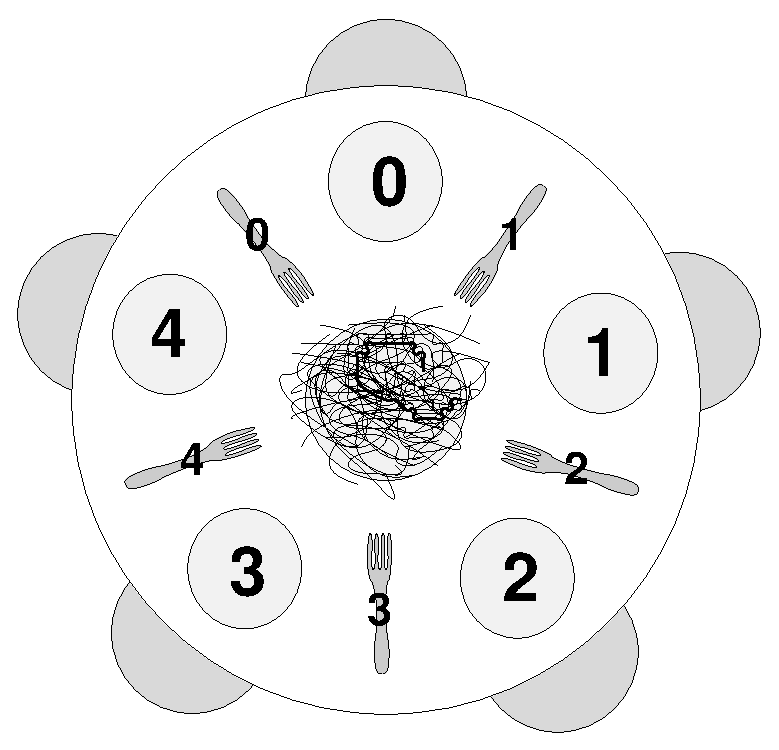
\includegraphics[height=2in]{table.eps}}

%Assuming that the philosophers know how to {\tt think} and {\tt eat},
%our job is to write a version of {\tt get\_forks} and {\tt put\_forks}
%that satisfies the following constraints:
    با فرض آنکه بدانیم فیلسوف‌ها چگونه {\tt think} و {\tt eat} می‌نمایند، وظیفه ما این است نسخه‌ای از {\tt get\_forks} و {\tt put\_forks}
    را بنویسیم که شرایط زیر را برآورده سازد:

\begin{itemize}

\item 
%Only one philosopher can hold a fork at a time.
    در یک زمان تنها یک فیلسوف بتواند یک چنگال را در اختیار داشته باشد. 

\item 
%It must be impossible for a deadlock to occur.
    امکان بروز بن‌بست وجود نداشته باشد. 

\item 
%It must be impossible for a philosopher to starve waiting for a fork.
    یک فیلسوف نباید به واسطه انتظار برای به دست آوردن یک چنگال دچار قحطی شود. 

\item 
%It must be possible for more than one philosopher
%to eat at the same time.
    این امکان وجود داشته باشد که بیش از یک فیلسوف بتوانند به صورت همزمان غذا خورند. 

\end{itemize}

%The last requirement is one way of saying that the solution
%should be efficient; that is, it should allow the maximum amount
%of concurrency.
    آخرین نیازمندی، بیان دیگری از این مطلب است که راه حل باید کارا باشد؛ به این معنی که باید حداکثر مقدار همروندی را اجازه دهد. 

%We make no assumption about how long {\tt eat} and {\tt think} take,
%except that {\tt eat} has to terminate eventually.  Otherwise, the
%third constraint is impossible---if a philosopher keeps one of the
%forks forever, nothing can prevent the neighbors from starving.
    درباره اینکه {\tt eat} و {\tt think} چقدر طول می‌کشد هیچ فرضی  در نظر نمی‌گیریم، بجز آنکه {\tt eat}  باید در نهایت خاتمه یابد. 
    در غیر اینصورت، اعمال محدودیت سوم ناممکن است---اگر یک فیلسوف یک از چنگال‌ها را تا ابد نگه دارد، هیچ چیز نمی‌تواند مانع قحطی همسایه‌ها شود. 
    

%To make it easy for philosophers to refer to their forks,
%we can use the functions {\tt left} and {\tt right}:
    برای اینکه ارجاع فیلسوف‌ها به چنگال‌هایشان را ساده نماییم می‌توانیم از توابع {\tt left} و {\tt right} استفاده کنیم. 

\begin{latin}
\begin{latin}
%\begin{lstlisting}[title={Which fork?}]{}
\begin{lstlisting}[title=\rl{کدام چنگال؟}]{}
def left(i): return i
def right(i): return (i + 1) % 5
\end{lstlisting}
\end{latin}
\end{latin}

%The {\tt \%} operator wraps around when it gets to 5, so
%{\tt (4 + 1) \% 5 = 0}.
    اپراتور {\tt \%} زمانیکه مقدار به ۵ برسد آن به ۰ بر می‌گرداند؛ {\tt (4 + 1) \% 5 = 0}.

%Since we have to enforce exclusive access to the forks,
%it is natural to use a list of Semaphores, one for
%each fork.  Initially, all the forks are available.
    از آنجایی که لازم است دسترسی انحصاری به چنگال‌ها را فراهم آوریم، طبیعی است که از لیستی از سمافورها استفاده کنیم، هر کدام برای یک چنگال. 
    در ابتدا تمامی چنگال‌ها موجودند. 

\begin{latin}
\begin{latin}
%\begin{lstlisting}[title={Variables for dining philosophers}]{}
\begin{lstlisting}[title=\rl{متغیرهای غذا خوردن فیلسوف‌ها}]{}
forks = [Semaphore(1) for i in range(5)]
\end{lstlisting}
\end{latin}
\end{latin}

%This notation for initializing a list might be unfamiliar to
%readers who don't use Python.  The {\tt range} function returns
%a list with 5 elements; for each element of this list, Python
%creates a Semaphore with initial value 1 and assembles the
%result in a list named {\tt forks}.    
    این نماد برای مقداردهی اولیه یک لیست ممکن است برای خوانندگانی که  پایتون را به کار نبرده‌اند ناآشنا باشد. 
    تابع {\tt range}، لیستی با پنج عنصر بر‌ می‌گرداند؛ برای هر عنصر این لیست، پایتون یک سمافور با مقدار اولیه ۱ ساخته و نتیجه را در یک لیست 
    به نام  {\tt forks} گرد می‌آورد.  

%Here is an initial attempt at {\tt get\_fork} and {\tt put\_fork}:
    تلاشی ابتدایی برای  {\tt get\_fork} و {\tt put\_fork} در ادامه آمده است:

\begin{latin}
\begin{latin}
%\begin{lstlisting}[title={Dining philosophers non-solution}]{}
\begin{lstlisting}[title=\rl{نا راه حل غذا خوردن فیلسوف}]{}
def get_forks(i):
    fork[right(i)].wait()
    fork[left(i)].wait()

def put_forks(i):
    fork[right(i)].signal()
    fork[left(i)].signal()
\end{lstlisting}
\end{latin}
\end{latin}

%It's clear that this solution satisfies the first constraint, but
%we can be pretty sure it doesn't satisfy the other two, because
%if it did, this wouldn't be an interesting problem and you would
%be reading Chapter~\ref{next}.
    واضح است که این راه حل اولین شرط را برآورده می‌نماید، امّا می‌توانیم مطمئن باشیم که دو شرط  بعدی برآورده نمی‌شود، زیرا که 
    اگر چنین بود، اصلاً مساله جذابی نبوده و شما می‌توانستید به مطالعه فصل~\ref{next} بپردازید. 

%Puzzle: what's wrong?
    معمّا:‌ مشکل کجاست؟


\clearemptydoublepage
%\subsection{Deadlock \#5}
\subsection{بن‌بست \#5}

%The problem is that the table is round.  As a result, each philosopher
%can pick up a fork and then wait forever for the other fork.  Deadlock!
    اشکال کار در این است که میز گرد است. در نتیجه، هر فیلسوف می‌تواند یک چنگال را بر گرفته و سپس برای همیشه منتظر چنگال دیگر بماند. بن‌بست! 

%Puzzle: write a solution to this problem that prevents deadlock.
    معمّا: راه حلی برای این مساله ارائه دهید که از بن‌بست جلوگیری نماید. 

%Hint: one way to avoid deadlock is to think about the conditions
%that make deadlock possible and then change one of those conditions.
%In this case, the deadlock is fairly fragile---a very small change
%breaks it.
    راهنمایی: یک راه اجتناب از بن‌بست این است که شرایطی که بن‌بست را ممکن می‌سازند را در نظر گرفته  و سپس یکی از آن‌ها را تغییر دهیم. 
    در این مورد، بن‌بست خیلی شکننده است--یک تغییر خیلی کوچک آن را در هم می‌شکند. 

\clearemptydoublepage
%\subsection{Dining philosophers hint \#1}
\subsection{راهنمایی غذا خوردن فیلسوف‌ها \#1}

%If only four philosophers are allowed at the table at a time,
%deadlock is impossible.
    اگر تنها چهار فیلسوف در یک زمان مجاز به نشستن سر میز باشند، بن‌بست غیر ممکن می‌گردد. 

%First, convince yourself that this claim is true, then write code that
%limits the number of philosophers at the table.
    ابتدا، خودتان را متقاعد نمایید که این ادعا درست است، سپس کدی بنویسید که تعداد فیلسوف‌ها را سر میز محدود نمایید. 


\clearemptydoublepage
%\subsection{Dining philosophers solution \#1}
\subsection{راه حل غذا خوردن فیلسوف‌ها  \#1}

%If there are only four philosophers at the table, then in the
%worst case each one picks up a fork.  Even then, there is a fork
%left on the table, and that fork has two neighbors, each of
%which is holding another fork.  Therefore, either of these
%neighbors can pick up the remaining fork and eat.
    اگر تنها چهار فیلسوف سر میز باشند، آنگاه در بدترین حالت هر کدام یک چنگال را بر می‌دارد. سپس، تنها یک چنگال روی میز باقی‌ مانده و 
    آن چنگال دو همسایه دارد که هر کدام یک چنگال دیگر در دست دارند. بنابراین، هر کدام از همسایه‌ها می‌توانند چنگال باقی‌مانده را برداشته و غذا خورد. 

%We can control the number of philosophers at the table with
%a Multiplex named {\tt footman} that is initialized to 4.
%Then the solution looks like this:
    تعداد فیلسوف‌های سر میز را می‌توانیم با مالتی‌پلکسی با نام {\tt footman} که مقدار اولیه ۴ دارد کنترل کنیم. 
    راه حل مشابه زیر است: 

\begin{latin}
\begin{latin}
%\begin{lstlisting}[title={Dining philosophers solution \#1}]{}
\begin{lstlisting}[title=\rl{راه حل غذا خوردن فیلسوف‌ها \#1}]{}
def get_forks(i):
    footman.wait()
    fork[right(i)].wait()
    fork[left(i)].wait()

def put_forks(i):
    fork[right(i)].signal()
    fork[left(i)].signal()
    footman.signal()
\end{lstlisting}
\end{latin}
\end{latin}

%In addition to avoiding deadlock, this solution also guarantees that
%no philosopher starves.
%Imagine that you
%are sitting at the table and both of your neighbors are eating.  You
%are blocked waiting for your right fork.  Eventually your right
%neighbor will put it down, because {\tt eat} can't run forever.  Since
%you are the only thread waiting for that fork, you will necessarily
%get it next.  By a similar argument, you cannot starve waiting for
%your left fork.
    علاوه بر اجتناب از بن‌بست، این راه حل تضمین می‌نماید که هیچ فیلسوفی دچار قحطی نشود. 
    تصور کنید که شما سر میز نشسته‌اید و هر دو همسایه شما مشغول غذا خوردن هستند. 
    شما در انتظار برای چنگال سمت راست مسدوده شده‌اید. در نهایتا همسایه سمت راست شما، چنگال را زمین خواهد گذاشت چرا که  {\tt eat} 
    نمی‌تواند تا ابد ادامه داشته باشد. از آنجاییکه شما تنها نخی هستید که منتظر آن چنگال هستید، لزوماً پس از آن چنگال به دست خواهید آورد. 
    با استدلالی مشابه، در انتظار برای چنگال سمت چپ‌تان نیز دچار قحطی نخواهید شد. 
    
%Therefore, the time a philosopher can spend at the table is bounded.
%That implies that the wait time to get into the room is also bounded,
%as long as {\tt footman} has Property 4 (see Section ~\ref{props}).
    بنابراین، زمانیکه یک فیلسوف می‌تواند سر میز بگذراد محدود است. همچنین این نکته دلالت بر این دارد که زمان انتظار برای ورود به اتاق 
    تا زمانیکه {\tt footman}  خصوصیت ۴ را دارد، محدود است (بخش ~\ref{props} را ببینید). 
     
    

%This solution shows that
%by controlling the number of philosophers, we can avoid deadlock.
%Another way to avoid deadlock is to change the order in which the
%philosophers pick up forks.  In the original non-solution, the
%philosophers are ``righties''; that is, they pick up the right fork
%first.  But what happens if Philosopher 0 is a leftie?
    این راه حل نشان می‌دهد که با کنترل کردن تعداد فیلسوف‌ها، می‌توانیم از بن‌بست اجتناب نماییم. 
    راه دیگر برای اجتناب از بن‌بست تغییر دادن ترتیبی است  که فیلسوف‌ها چنگال‌ها را بر می‌دارند. 
    در نا راه حل اولیه، فیلسوف‌ها "راست‌دست``\LTRfootnote{} هستند؛ به این معنی که ابتدا چنگال سمت راست را بر می‌دارند. 
    امّا اگر فیلسوف ۰ "چپ‌دست``\LTRfootnote{} باشد چه اتفاقی می‌افتد؟‌

%Puzzle: prove that if there is at least one leftie and at least one
%rightie, then deadlock is not possible.
    معمّا: ثابت کنید که اگر حداقل یکی از فیلسوف‌ها چپ‌دست و حداقل یکی راست‌دست باشد، آنگاه بن‌بست غیر ممکن است. 

%Hint: deadlock can only occur when all 5 philosophers are holding
%one fork and waiting, forever, for the other.  Otherwise, one of
%them could get both forks, eat, and leave.
    راهنمایی: بن‌بست تنها زمانی رخ می‌دهد که ۵ فیلسوف یک چنگال را برای در دست دارند و تا ابد منتظر چنگال دیگر می‌مانند. 
    در غیر اینصورت، یکی از آن‌ها می‌تواند هر دو چنگال را برداشته، غذا خورده و خارج شود. 

%The proof works by contradiction.  First, assume that deadlock is
%possible.  Then choose one of the supposedly deadlocked philosophers.
%If she's a leftie, you can prove that the philosophers are all
%lefties, which is a contradiction.  Similarly, if she's a rightie, you
%can prove that they are all righties.  Either way you get a
%contradiction; therefore, deadlock is not possible.
    اثبات با برهان خلف است.  ابتدا، تصور کنید که بن‌بست ممکن باشد. 
    سپس یکی از فیلسوف‌هایی که در بن‌بست گیر کرده است انتخاب نمایید. 
    اگر آن فیلسوف چپ‌دست باشد،‌ می‌توانید ثابت نمایید که تمامی‌ فیلسوف‌ها چپ‌دست هستند، که این خود یک تناقض است. 
    به طور مشابه، اگر راست‌دست باشد می‌تواند ثابت نمایید که همگی راست‌دست هستند. از هر دو طریق به تناقض می‌رسید؛ بنابراین 
    بن‌بست ناممکن است. 
    
%%%%    Sat 11 Nov 2017 06:20:18 PM +0330

\clearemptydoublepage
%\subsection{Dining philosopher's solution \#2}
\subsection{راه حل غذاخوردن فیلسوف‌ها \#2}

%In the asymmetric solution to the Dining philosophers problem,
%there has to be at least one leftie and at least one rightie at
%the table.  In that case, deadlock is impossible.  The previous
%hint outlines the proof.  Here are the details.
    در راه حل متقارن مساله غذاخوردن فلیسوف‌ها، لازم است حداقل یک چپ دست و  حداقل یک راست دست سر میز باشند. 
    در این حالت، بن‌بست غیر ممکن است. راهنمایی قبل طرح کلی اثبات را بیان می‌کند.
    در ادامه جزئیات آمده است. 

%Again, if deadlock is possible, it occurs when all 5 philosophers
%are holding one fork and waiting for the other.  If we assume that
%Philosopher $j$ is a leftie, then she must be holding her left
%fork and waiting for her right.  Therefore her neighbor to the right,
%Philosopher $k$, must be holding his left fork and waiting for
%his right neighbor; in other words, Philosopher $k$ must be a leftie.
%Repeating the same argument, we can prove that the philosophers
%are all lefties, which contradicts the original claim that there
%is at least one rightie.  Therefore deadlock is not possible.
    دوباره، اگر بن‌بست ممکن باشد، زمانی رخ می‌دهد که تمامی ۵ فیلسوف یک چنگال را نگاه داشته و منتظر چنگال دیگر بمانند. 
    اگر فرض کنیم فیلسوف $j$ چپ دست باشد آنگاه او باید چنگال سمت چپ را نگاه داشته و منتظر چنگال سمت راست باشد. 
    بنابراین همسایه سمت راست او (فیلسوف $k$) باید چنگال سمت چپش را نگاه داشته و منتظر همسایه راست خود باشد؛ به عبارت دیگر 
    فیلسوف $k$ باید چپ دست باشد. با تکرار استدلال مشابه می‌توانیم ثابت کنیم که تمامی فیلسوف‌ها چپ دست هستند که با حکم اولیه که در آن 
    حداقل یک راست دست وجود دارد در تناقض است. لذا بن‌بست ممکن نیست. 

%The same argument we used for the previous solution also proves
%that starvation is impossible for this solution.
    استدلالی مشابه آنچه برای راه حل قبل به کار بردیم ثابت می‌کند که قطحی نیز غیر ممکن است. 


\clearemptydoublepage
%\subsection{Tanenbaum's solution}
\subsection{راه حل تننبام}

%There is nothing wrong with the previous solutions, but just for
%completeness, let's look at some alternatives.  One of the best known
%is the one that appears in Tanenbaum's popular operating systems
%textbook \cite{tanenbaum}.
%For each philosopher there is a state variable that
%indicates whether the philosopher is thinking, eating, or waiting to
%eat (``hungry'') and a semaphore that indicates whether the
%philosopher can start eating.  Here are the variables:
    در راه حل قبل هیچ چیز نادرستی وجود ندارد امّا تنها برای تکمیل بحث، بگذارید نگاهی به برخی راه حل‌های جایگزین بیندازیم. 
    یکی از شناخته‌ شده ترینِ  این راه حل‌ها، همانی است که در کتاب معروف سیستم‌عامل تننبام آمده است\cite{tanenbaum}. 
    برای هر فیلسوف یک متغیر وضعیت وجود دارد که نشان می‌دهد فیلسوف در کدامیک از حالات تفکر، خوردن و یاد انتظار برای خوردن (گرسنگی) است و 
    یک سمافور که نشان می‌دهد آیا فیلسوف می‌تواند غذا خوردن را آغاز نماید نیز وجود دارد. 

\begin{latin}
\begin{latin}
%\begin{lstlisting}[title={Variables for Tanenbaum's solution}]{}
\begin{lstlisting}[title=\rl{متغیرهای راه حل تننبام}]{}
state = ['thinking'] * 5
sem = [Semaphore(0) for i in range(5)]
mutex = Semaphore(1)
\end{lstlisting}
\end{latin}
\end{latin}

%The initial value of {\tt state} is a list of 5 copies of {\tt
%'thinking'}.  {\tt sem} is a list of 5 semaphores with the initial
%value 0.  Here is the code:
    مقدار اولیه {\tt state} یک لیست ۵ تایی از {\tt 'thinking'} است.     {\tt sem}
    یک لیست ۵ تایی از سمافورهایی است با مقدار اولیه ۰. 
    و امّا کد: 

\begin{latin}
\begin{latin}
%\begin{lstlisting}[title={Tanenbaum's solution}]{}
\begin{lstlisting}[title=\rl{ راه حل تننبام}]{}
def get_fork(i):
    mutex.wait()
    state[i] = 'hungry'
    test(i)
    mutex.signal()
    sem[i].wait()

def put_fork(i):
    mutex.wait()
    state[i] = 'thinking'
    test(right(i))
    test(left(i))
    mutex.signal()

def test(i):
    if state[i] == 'hungry' and
    state[left (i)]  != 'eating' and
    state[right (i)] != 'eating':
        state[i] = 'eating'
        sem[i].signal()
\end{lstlisting}
\end{latin}
\end{latin}

% NOTE: need to fix this; see email from David Furcy.

%The {\tt test} function checks whether the $i$th philosopher can
%start eating, which he can if he is hungry and
%neither of his neighbors are eating.  If so, the {\tt test} signals
%semaphore $i$.
    تابع {\tt test}  بررسی می‌کند که آیا فیلسوف $i$ام می‌تواند شروع به غذا خوردن نماید، و این در صورتی است که 
    او گرسنه بوده و هیچکدام از همسایه‌هایش در حال غذا خوردن نباشند. اگر چنین باشد، {\tt test} به سمافور $i$ سیگنال می‌دهد. 
    
%There are two ways a philosopher gets to eat.  In the first case, the
%philosopher executes {\tt get\_forks}, finds the forks available, and
%proceeds immediately.  In the second case, one of the neighbors is
%eating and the philosopher blocks on its own semaphore.  Eventually,
%one of the neighbors will finish, at which point it executes {\tt
%test} on both of its neighbors.  It is possible that both tests
%will succeed, in which case the neighbors can run concurrently.
%The order of the two tests doesn't matter.
    دو راه وجود دارد که یک فیلسوف می‌تواند غذا بخورد. در حالت اول، فیلسوف {\tt get\_forks} را اجرا کرده، چنگال‌های موجود را یافته و 
    بلافاصله مشغول خوردن می‌شود. در حالت دوم، یکی از همسایه‌ها در حال غذا خوردن است و فیلسوف روی سمافور خودش مسدود گردیده است. 
    نهایتاً یکی از همسایه‌ها دست از غذا می‌کشد و در این زمان  {\tt test} را روی هر دو همسایه خود اجرا می‌نماید. 
    ممکن است که هر دو بررسی موفقیت آمیز باشد، و در این حالت همسایه‌ها می‌توانند به صورت همروند مشغول غذا خوردن شوند. 
    ترتیب دو بررسی اهمیتی ندارد. 

%In order to access {\tt state} or invoke {\tt test}, a thread
%has to hold {\tt mutex}.  Thus, the operation of checking and
%updating the array is atomic.  Since a philosopher can only proceed
%when we know both forks are available, exclusive access to the forks
%is guaranteed.
    به منظور دسترسی به {\tt state} یا فراخوانی {\tt test}، یک نخ باید {\tt mutex} را بگیرد. 
    بنابراین، عمل بررسی و بروزرسانی آرایه، اتمی است.از آنجایی که یک فیلسوف تنها زمانی می‌تواند مشغول خوردن شود که بدانیم هر دو چنگال موجود است، 
    دسترسی انحصاری به چنگال‌ها تضمین شده است. 

%No deadlock is possible, because the only semaphore that is accessed
%by more than one philosopher is {\tt mutex}, and no thread executes
%{\tt wait} while holding {\tt mutex}.
    هیچ بن‌بستی ممکن نیست، زیرا تنها سمافوری که بیش از یک فیلسوف به آن دسترسی دارد، {\tt mutex} است و هیچ نخی  
    تا زمانی که {\tt mutex} را در اختیار دارد {\tt wait} را اجرا نمی‌نماید. 

%But again, starvation is tricky.
    امّا دومرتبه، قطحی ممکن ولی در اینجا خیلی مستلزم دقت و مهارت است.

%Puzzle: Either convince yourself that Tanenbaum's solution prevents
%starvation or find a repeating pattern that allows a thread to starve
%while other threads make progress.
    معمّا: یا خودتان را متقاعد نمایید راه حل تننبام از قحطی جلوگیری می‌نماید و یا یک الگوی تکرارشونده بیابید اجازه می‌دهد یک نخ دچار قحطی شود 
    در حالیکه مابقی نخ‌ها به کار خود ادامه می‌دهند. 


\clearemptydoublepage
%\subsection{Starving Tanenbaums}
\subsection{قطحی تننبام}

%Unfortunately, this solution is not starvation-free.  Gingras
%demonstrated that there are repeating patterns that allow a
%thread to wait forever while other threads come and go
%\cite{gingras90dining}.
    متاسفانه، این راه حل مصون از قحطی نیست. \lr{Gingras} نشان داد که الگوهای تکرارشونده‌ای وجود دارد در آن یک نخ برای همیشه منتظر مانده در 
    حالیکه دیگر نخ‌ها می‌آیند و می‌روند\cite{gingras90dining}.

%Imagine that we are trying to starve Philosopher 0.  Initially,
%2 and 4 are at the table and 1 and 3 are hungry.  Imagine that 2 gets up and
%1 sit downs; then 4 gets up and 3 sits down.
%Now we are in the mirror image of the starting position.
    تصور کنید که می‌خواهیم فیلسوف ۰ دچار قطحی شود. در ابتدا، ۲ و ۴ سر میز هستند و ۱ و ۳ گرسنه هستند. تصور کنید که ۲ بر می‌خیزد و یک سر میز می‌نشیند؛ 
    سپس ۴ برخواسته و ۳ می‌نشیند. اکنون در وضعیتی قرینه موقعیت شروع هستیم. 

%If 3 gets up and 4 sits
%down, and then 1 gets up and 2 sits down, we are back
%where we started.  We could repeat the cycle indefinitely and
%Philosopher 0 would starve.
    اگر ۳ برخیزد و ۴ بنشیند، و سپس  برخواسته و ۲ بنشیند، به نقطه شروع بازگشته‌ایم. 
    این  حلقه را می‌توانیم تا ابد تکرار نماییم و در این صورت فیلسوف ۰ دچار قحطی می‌شود. 

%So, Tanenbaum's solution doesn't satisfy all the requirements.
    لذا راه حل تننبام تمامی ملزومات را بار آورده نمی‌نماید. 


\clearemptydoublepage
%\section {Cigarette smokers problem}
\section {مساله سیگاری‌ها}

%The cigarette smokers problem was originally presented by
%Suhas Patil \cite{patil}, who claimed that it cannot be solved with
%semaphores.  That claim comes with some qualifications, but in
%any case the problem is interesting and challenging.
    مساله سیگاری‌ها در ابتدا توسط     \lr{Suhas Patil} مطرح شد \cite{patil}، و ادعا نمود که  این مساله به سمافورها قابل حل نیست. 
    این ادعا با تعدادی شرط همراه است، امّا در هر حالت مساله جذاب و چالش برانگیز است. 

%Four threads are involved: an agent and three smokers.  The smokers
%loop forever, first waiting for ingredients, then making and smoking
%cigarettes.  The ingredients are tobacco, paper, and matches.
    چهار نخ در مساله وجود دارد: یک عامل و سه سیگاری. سیگاری‌ها تا ابد، در حلقهٔ ابتدا انتظار برای مواد مورد نیاز و سپس ساختن و کشیدن سیگار هستند.
    مواد مورد نیاز شامل تنباکو، کاغذ و کبریت است. 

%We assume that the agent has an infinite supply of all three
%ingredients, and each smoker has an infinite supply of one of
%the ingredients; that is, one smoker has matches, another has
%paper, and the third has tobacco.
    فرض می‌کنیم که عامل یک منبع لایزال از این سه ماده لازم دارد و هر سیگاری یک منبع نامتناهی از یکی از این سه مواد لازم را دارد، بدین معنی که 
    یکی از سیگاری‌ها کبریت، دیگری کاغذ و سومی نیز تنباکو دارد. 

%The agent repeatedly chooses two different ingredients at random
%and makes them available to the smokers.  Depending on which
%ingredients are chosen, the smoker with the complementary ingredient
%should pick up both resources and proceed.
    عامل مکراراً دو ماده متفاوت را به صورت تصادفی انتخاب نموده و آن‌ها را به سیگاری‌ها عرضه می‌کند. 
    بسته به اینکه چه موادی انتخاب شده باشد، فرد سیگاری با ماده مکمل خود می‌تواند دو منبع را برداشته و ادامه دهد. 

%For example, if the agent puts out tobacco and paper, the
%smoker with the matches should pick up both ingredients, make
%a cigarette, and then signal the agent.
    برای مثال، اگر عامل تنباکو و کاغذ بر دارد، فرد سیگاری که کبریت دارد می‌تواند هر دو ماده را برداشته و یک سیگار ساخته و سپس به عامل سیگنال دهد. 

%To explain the premise, the agent represents an operating system that
%allocates resources, and the smokers represent applications that need
%resources.  The problem is to make sure that if resources are
%available that would allow one more applications to proceed,
%those applications should be woken up.  Conversely, we want to avoid
%waking an application if it cannot proceed.
    برای توضیح فرض قبل،‌    
    عامل نشانگر یک سیستم‌عامل است که منابع را تخصیص می‌دهد، و سیگاری‌ها نشانگر برنامه‌هایی هستند که به منابع نیاز دارند. 
    مساله این است که اطمینان دهیم اگر منابعی موجود هستند که می‌توانند اجازه ادامه فعالیت برنامه‌های بیشتری را بدهند آن برنامه‌ها باید بیدار شوند. 
    بر عکس، می‌خواهیم از بیدار نمودن برنامه‌هایی که نمی‌توانند به کار خود ادامه دهند اجتناب نماییم. 


%Based on this premise, there are three versions of this problem
%that often appear in textbooks:
    بر طبق این فرض، سه نسخه از این مساله وجود دارد که اغلب در کتاب‌ها مشاهده می‌شود: 

\begin{description}

\item
%[The impossible version:] Patil's version imposes restrictions on
%the solution.  First, you are not allowed to modify the agent code.
%If the agent represents an operating system, it makes sense to assume
%that you don't want to modify it every time a new application comes
%along.  The second restriction is that you can't use conditional
%statements or an array of semaphores.  With these constraints, the
%problem cannot be solved, but as Parnas points out, the second
%restriction is pretty artificial \cite{Parnas}.  With constraints like
%these, a lot of problems become unsolvable.
    [نسخه غیرممکن:] نسخه \lr{Patil} محدودیت‌هایی روی راه حل تحمیل می‌نماید. اول اینکه، شما اجازه تغییر کد عامل را ندارید. 
    اگر عامل نشانگر یک سیستم‌عامل باشد، این فرض که شما نمی‌خواهید کد سیستم عامل را هر زمان که یک برنامه جدید می‌آید تغییر دهید بی معنی نیست. 
    محدودیت دوم این است که شما نمی‌توانید از عبارات شرطی یا یک آرایه‌ای از سمافورها استفاده نمایید. با این محدودیت‌ها، 
    مساله قابل حل نیست، امّا همانطور که  \lr{Patil} اشاره نموده است محدودیت دوم کاملاً تصنعی است  \cite{Parnas}. 
    با محدودیت‌هایی نظیر این دو، مسائل بسیار غیر قابل حل خواهد شد. 

\item
%[The interesting version:] This version keeps the first
%restriction---you can't change the agent code---but it drops the others.
    [نسخه جالب:] این نسخه محدودیت اول (عدم امکان تغییر کد عامل) را دارد ولی مابقی را در نظر نمی‌گیرد.
    
\item
%[The trivial version:] In some textbooks, the problem specifies
%that the agent should signal the smoker that should go next, according
%to the ingredients that are available.  This version of the problem
%is uninteresting because it makes the whole premise, the ingredients
%and the cigarettes, irrelevant.  Also, as a practical matter, it is
%probably not a good idea to require the agent to know about the other
%threads and what they are waiting for.  Finally, this version of
%the problem is just too easy.
    [نسخه بدیهی:] در برخی کتاب‌ها، در خود مساله آمده است که عامل باید بر مبنای مواد موجود به آن فرد سیگاری که می‌تواند ادامه دهد سیگنال ارسال نماید. 
    این نسخه از مساله، جذابیتی ندارد زیرا که تمام فرض اولیه، مواد افزودنی و سیگارها را غیرضروری می‌نماید. همچنین در عمل، احتمالاً     
     اینکه عامل، اطلاعی از سایر نخ‌ها و آنچه آن‌ها نیاز دارند داشته باشد ایده خوبی نباشد. در نهایت،  این نسخه از مساله نیز بسیار ساده است.
     
\end{description}
%%%%        Sat 18 Nov 2017 06:11:58 PM +0330

%Naturally, we will focus on the interesting version.  To complete
%the statement of the problem, we need to specify the agent code.
%The agent uses the following semaphores:
    طبیعتاً بر روی نسخه جالب تمرکز می‌نمایم. برای تکمیل بیان مساله، باید کد عامل را مشخص نماییم. عامل، سمافورهای زیر را بکار می‌برد:

\begin{latin}
\begin{latin}
%\begin{lstlisting}[title={Agent semaphores}]{}
\begin{lstlisting}[title=\rl{سمافورهای عامل}]{}
agentSem = Semaphore(1)
tobacco = Semaphore(0)
paper = Semaphore(0)
match = Semaphore(0)
\end{lstlisting}
\end{latin}
\end{latin}

%The agent is actually made up of three concurrent
%threads, Agent A, Agent B and Agent C.  Each waits on
%{\tt agentSem}; each time {\tt agentSem} is signaled,
%one of the Agents wakes up and provides ingredients by
%signaling two semaphores.
    عامل در واقع از سه نخ همروند تشکیل شده است:  عامل \lr{A}،  عامل \lr{B}،  عامل \lr{C}.
    هر کدام از آن‌ها روی {\tt agentSem} منتظر می‌مانند؛ هر گاه که {\tt agentSem} سیگنالی دریافت کند، یکی از عامل‌ها بر می‌خیزد و 
    از طریق سیگنال‌دهی به دو سمافور، مواد مورد نیاز را فراهم می‌آورد. 

\begin{latin}
\begin{latin}
%\begin{lstlisting}[title={Agent A code}]{}
\begin{lstlisting}[title=\rl{کد عامل \lr{A}}]{}
agentSem.wait()
tobacco.signal()
paper.signal()
\end{lstlisting}
\end{latin}


\begin{latin}
%\begin{lstlisting}[title={Agent B code}]{}
\begin{lstlisting}[title=\rl{کد عامل \lr{B}}]{}
agentSem.wait()
paper.signal()
match.signal()
\end{lstlisting}
\end{latin}

\begin{latin}
%\begin{lstlisting}[title={Agent C code}]{}
\begin{lstlisting}[title=\rl{کد عامل \lr{C}}]{}
agentSem.wait()
tobacco.signal()
match.signal()
\end{lstlisting}
\end{latin}
\end{latin}

%This problem is hard because the natural solution does not
%work.  It is tempting to write something like:
    این مساله آنقدرها هم ساده نیست و راه حل طبیعی آن کار نمی‌کند. نوشتن کدی مانند زیر، وسوسه انگیز است: 
    

\begin{latin}
\begin{latin}
%\begin{lstlisting}[title={Smoker with matches}]{}
\begin{lstlisting}[title=\rl{سیگاری با کبریت}]{}
tobacco.wait()
paper.wait()
agentSem.signal()
\end{lstlisting}
\end{latin}

\begin{latin}
%\begin{lstlisting}[title={Smoker with tobacco}]{}
\begin{lstlisting}[title=\rl{سیگاری با تنباکو}]{}
paper.wait()
match.wait()
agentSem.signal()
\end{lstlisting}
\end{latin}

\begin{latin}
%\begin{lstlisting}[title={Smoker with paper}]{}
\begin{lstlisting}[title=\rl{سیگاری با کاغذ}]{}
tobacco.wait()
match.wait()
agentSem.signal()
\end{lstlisting}
\end{latin}
\end{latin}

%What's wrong with this solution?
    مشکل این  راه حل کجاست؟

\clearemptydoublepage
%\subsection{Deadlock \#6}
\subsection{بن‌بست \#6}

%The problem with the previous solution is the possibility
%of deadlock.  Imagine that the agent puts out tobacco and
%paper.  Since the smoker with matches is waiting on {\tt tobacco},
%it might be unblocked.  But the smoker with tobacco is
%waiting on {\tt paper}, so it is possible (even likely) that
%it will also be unblocked.  Then the first thread will block
%on {\tt paper} and the second will block on {\tt match}.
%Deadlock!
    مشکل راه حل قبل امکان وقوع بن‌بست است. تصور کنید که عامل تنباکو و کاغذ عرضه می‌نماید. از آنجایی که فرد  سیگاری‌ که در دست خود کبریت دارد 
    منتظر {\tt tobacco} ممکن است رفع انسداد گردد. امّا آن فرد سیگاری که در دست خود تنباکو دارد منتظر {\tt paper} است، لذا ممکن است او نیز 
    رفع انسداد گردد (احتمال آن نیز زیاد است). سپس اولین نخ روی {\tt paper} مسدود گردیده و دومی نیز روی {\tt match} مسدود می‌گردد و بن‌بست!. 

\clearemptydoublepage
%\subsection{Smokers problem hint}
\subsection{راهنمایی مساله سیگاری‌ها}

%The solution proposed by Parnas uses three helper threads
%called ``pushers'' that respond to the signals from the agent,
%keep track of the available ingredients, and signal the
%appropriate smoker.
    راه حل \lr{Parnas}، "سه نخ کمکی فروشندهٔ غیر مجاز``\LTRfootnote{pusher} را به کار می‌برد که آن‌ها به سیگنال‌هایی که از عامل‌
    می‌رسد پاسخ می‌دهند، میزان موجود مواد مورد نیاز را نگه می‌دارند و به سیگاری مناسب سیگنال می‌دهند. 

%The additional variables and semaphores are
    متغیرها و سمافورهای اضافی به شرح زیر است: 

\begin{latin}
\begin{latin}
%\begin{lstlisting}[title={Smokers problem hint}]{}
\begin{lstlisting}[title=\rl{راهنمایی مساله سیگاری‌ها}]{}
isTobacco = isPaper = isMatch = False
tobaccoSem = Semaphore(0)
paperSem = Semaphore(0)
matchSem = Semaphore(0)
\end{lstlisting}
\end{latin}
\end{latin}

%The boolean variables indicate whether or not an ingredient
%is on the table.  The pushers use {\tt tobaccoSem} to signal
%the smoker with tobacco, and the other semaphores likewise.
    متغیرهای بولی نشان می‌دهند که آیا یک ماده مورد نظر وجود دارد یا خیر. 
    فروشنده‌‌ها {\tt tobaccoSem} را بکار برده تا به آن فرد سیگاری که تنباکو در دست دارد سیگنال بدهد و به طرقی مشابه به سمافورهای دیگر. 


\clearemptydoublepage
%\subsection{Smoker problem solution}
\subsection{راه حل مساله سیگاری}

%Here is the code for one of the pushers:
    کد یکی از فروشندگان در ادامه آمده است:‌

\begin{latin}
\begin{latin}
%\begin{lstlisting}[title={Pusher A}]{}
\begin{lstlisting}[title=\rl{فروشنده \lr{A}}]{}
tobacco.wait()
mutex.wait()
    if isPaper:
        isPaper = False
        matchSem.signal()
    elif isMatch:
        isMatch = False
        paperSem.signal()
    else: 
        isTobacco = True
mutex.signal()
\end{lstlisting}
\end{latin}
\end{latin}

%This pusher wakes up any time there is tobacco on the
%table.  If it finds {\tt isPaper} true, it knows that
%Pusher B has already run, so it can signal the smoker
%with matches.  Similarly, if it finds a match on the
%table, it can signal the smoker with paper.
    این فروشنده هر زمان که تنباکو موجود باشد فعال می‌شود. اگر مقدار {\tt isPaper} برابر \lr{true} باشد، می‌داند که فروشندهٔ‌ \lr{B} نیز در حال 
    حاضر فعال است، لذا می‌تواند به آن فرد سیگاری که در دست خود کبریت دارد سیگنال دهد. به طور مشابه، اگر کبریت موجود باشد می‌تواند به آن فرد 
    سیگاری که در دست خود کاغذ دارد سیگنال دهد. 

%But if Pusher A runs first, then it will find both
%{\tt isPaper} and {\tt isMatch} false.  It cannot signal
%any of the smokers, so it sets {\tt isTobacco}.
    اگر نسخت فروشنده \lr{A} اجرا شود، سپس هر دوی {\tt isPaper} و  {\tt isMatch}  را \lr{false} می‌بیند و نمی‌تواند به هیچ‌کدام از افراد 
    سیگاری سیگنال دهد لذا مقدار  {\tt isTobacco} را \lr{true}  می‌نماید. 

%The other pushers are similar.  Since the pushers do all
%the real work, the smoker code is trivial:
    فروشنده‌های دیگر نیز چنین هستند. از آنجایی که  تمام کار اصلی را فروشنده‌ها انجام می‌دهند، کد سیگاری بدیهی می‌شود.

\begin{latin}
\begin{latin}
%\begin{lstlisting}[title={Smoker with tobacco}]{}
\begin{lstlisting}[title=\rl{فرد سیگاری با تنباکو}]{}
tobaccoSem.wait()
makeCigarette()
agentSem.signal()
smoke()
\end{lstlisting}
\end{latin}
\end{latin}

%Parnas presents a similar solution that assembles the
%boolean variables, bitwise, into an integer, and then
%uses the integer as an index into an array of semaphores.
%That way he can avoid using conditionals (one of the
%artificial constraints).  The resulting code is a bit
%more concise, but its function is not as obvious.
    \lr{Parnas}
    راه حل مشابهی ارائه می‌دهد که متغیرهای بولی را به صورت بیتی در یک متغیر صحیح ذخیره نموده است و سپس عدد صحیح را به عنوان 
    اندیس آرایه‌ای از سمافورها بکار می‌بندد. با این شیوه، راه حل او از شرط (یکی از محدودیت‌های تصنعی) اجتناب می‌نماید. 
    کد حاصل کمی خلاصه‌تر است، امّا عملکردش آنقدر واضح نیست. 
    
%%%    Sun 26 Nov 2017 05:59:38 PM +0330

%\subsection{Generalized Smokers Problem}
\subsection{تعمیم مساله سیگاری‌ها}

%Parnas suggested that the smokers problem becomes more
%difficult if we modify the agent, eliminating the requirement
%that the agent wait after putting out ingredients.  In this
%case, there might be multiple instances of an ingredient on
%the table.
    \lr{Parnas} پیشنهاد نمود که اگر عامل را به این صورت دستکاری کنیم 
    که نیازی نباشد که عامل پس از گذاشتن مواد لازم صبر نماید، آنگاه مساله سیگاری‌ها دشوارتر خواهد می‌گردد. 
    در این حالت، باید چند نمونه از یک ماده روی میز موجود باشد. 

%Puzzle: modify the previous solution to deal with this
%variation.
    معمّا: راه حل قبل را به گونه‌ای دستکاری کنید که با این تغییر مطابقت داشته باشد. 

\clearemptydoublepage
%\subsection{Generalized Smokers Problem Hint}
\subsection{راهنمای تعمیم مساله سیگاری‌ها}

%If the agents don't wait for the smokers, ingredients might
%accumulate on the table.  Instead of using boolean values to
%keep track of ingredients, we need integers to count them.
    اگر عامل، منتظر سیگاری‌ها نماند، ممکن است موارد لازم روی میز انباشته شود. بجای استفاده از مقادیر بولی به منظور ردگیری موارد لازم، 
    به اعداد صحیح برای شمارش آن‌ها نیاز داریم. 

\begin{latin}
\begin{latin}
\begin{lstlisting}[title=\rl{راهنمای تعمیم مساله سیگاری‌ها}]
numTobacco = numPaper = numMatch = 0
\end{lstlisting}
\end{latin}
\end{latin}


\clearemptydoublepage
%\subsection{Generalized Smokers Problem Solution}
\subsection{راه حل تعمیم‌یافته مساله سیگاری‌ها}
\label{smoker}

%Here is the modified code for Pusher A:
    کد تغییر یافته فروشنده \lr{A} در ادامه آمده است: 

\begin{latin}
\begin{latin}
%\begin{lstlisting}[title={Pusher A}]{}
\begin{lstlisting}[title={\rl{فروشنده} A}]{}
tobacco.wait()
mutex.wait()
    if numPaper:
        numPaper -= 1
        matchSem.signal()
    elif numMatch:
        numMatch -= 1
        paperSem.signal()
    else: 
        numTobacco += 1
mutex.signal()
\end{lstlisting}
\end{latin}
\end{latin}

%One way to visualize this problem is to imagine that when an
%Agent runs, it creates two pushers, gives each of them one ingredient,
%and puts them in a room with all the other pushers.  Because of the
%mutex, the pushers file into a room where there are
%three sleeping smokers and a table.  One at a time, each pusher enters
%the room and checks the ingredients on the table.  If he can
%assemble a complete set of ingredients, he takes them off the table
%and wakes the corresponding smoker.  If not, he leaves his ingredient
%on the table and leaves without waking anyone.
    یک راه تصویرسازی این مساله این است که تصویر نمایید آنزمان که عاملی اجرا می‌شود‌، دو فروشنده ساخته و به هر کدام از آن‌ها یکی از مواد لازم را 
    می‌دهد و آن‌ها را همراه با سایر فروشندگان در یک اتاق قرار می‌دهد. به سبب میوتکس، فروشنده‌ها در اتاقی که سه سیگاری خوابیده و یک میز وجود دارد 
    به ترتیب وارد می‌شوند. هر فروشنده یکی پس از دیگری وارد اتاق شده و مواد روی میز را بررسی می‌نماید. اگر او بتواند یک مجموعه کامل از مواد لازم سیگار را
    گرد آورد، آن‌ها از روی میز برداشته و سیگاری متناظر را بیدار می‌نماید. و اگر نتواند،‌ مواد همراه خود را روی میز رها کرده و اتاق را بدون اینکه کسی را 
    بیدار کند ترک می‌نماید. 

%This is an example of a pattern we will see several times, which
%I call a {\bf scoreboard}.  The variables {\tt numPaper}, {\tt numTobacco}
%and {\tt numMatch} keep track of the state of the system.  As each
%thread files through the mutex, it checks the state as if looking
%at the scoreboard, and reacts accordingly.
    این مثالی از الگویی است که آن را «جدول امتیاز»\LTRfootnote{scoreboard} خوانده و بعداً چندین مرتبه آن را خواهیم دید.   
    متغیرهای     {\tt numPaper}، {\tt numTobacco} و  {\tt numMatch}    وضعیت سیستم را نگاه می‌دارند. 
    از آنجایی که هر نخ از طریق میوتکس به ترتیب وارد می‌شود، مثل اینکه به جدول امتیاز نگاه کرده باشد وضعیت را بررسی نموده و مطابق آن عکس العمل نشان می‌دهد. 


\clearemptydoublepage
%\chapter{Less classical synchronization problems}
\chapter{مسائل همگام‌سازی کمتر-کلاسیک}
\label{next}


%\section{The dining savages problem}
\section{مساله غذاخوردن وحشی‌ها}

%This problem is from Andrews's 
%{\em Concurrent Programming} \cite{andrews}.
    این مساله از  \emph{برنامه‌نویسی همروند} \lr{Andrews}  اقتباس شده است\cite{andrews}. 

\begin {quotation}
%A tribe of savages eats communal dinners from a large pot that can
%hold M servings of stewed missionary\footnote{This problem is based on
%a cartoonish representation of the history of Western missionaries
%among hunter-gatherer societies.  Some humor is intended by the
%allusion to the Dining Philosophers problem, but the representation of
%``savages'' here isn't intended to be any more realistic than the
%previous representation of philosophers.  If you are interested in
%hunter-gatherer societies, I recommend Jared Diamond's {\em Guns,
%Germs and Steel}, Napoleon Chagnon's {\em The Yanomamo}, and Redmond
%O'Hanlon's {\em In Trouble Again}, but not Tierney's {\em Darkness in
%El Dorado}, which I believe is unreliable.}.  When a savage wants to
%eat, he helps himself from the pot, unless it is empty.  If the pot is
%empty, the savage wakes up the cook and then waits until the cook has
%refilled the pot.
    قبیله‌ای از وحشی‌ها، از یک دیگ بزرگ که می‌تواند \lr{M}  پرس ازمُبلّغ پخته شده را در خود نگاه دارد به صورت مشترک شام می‌خورند.
%    \footnote{
%    این مساله برای پایه نمایش کارتونی تاریخ مبلغین غربی در میان جوامع تشکیل شده با محوریت شکار است. مقداری طنز با کنایه به مساله غذاخوردن فلیسوف‌ها 
%    تعمداً      }. 
    زمانیکه یک وحشی می‌خواهد غذا بخورد، از درون دیگ از خود پذیرایی می‌کند مگر اینکه دیگ خالی باشد. 
    اگر دیگ خالی بود، وحشی آشپز را بیدار نموده و سپس منتظر او می‌ماند تا دومرتبه دیگر را پر نماید.
\end{quotation}

%Any number of savage threads run the following code:
    هر تعداد نخ وحشی می‌تواند کد زیر را اجرا نماید:

\begin{latin}
\begin{latin}
%\begin{lstlisting}[title={Unsynchronized savage code}]{}
\begin{lstlisting}[title=\rl{کد ناهمگام یک وحشی}]{}
while True:
    getServingFromPot()
    eat()
\end{lstlisting}
\end{latin}
\end{latin}

%And one cook thread runs this code:
    و نخ یک آشپز کد زیر را اجرا می‌نماید:

\begin{latin}
\begin{latin}
%\begin{lstlisting}[title={Unsynchronized cook code}]{}
\begin{lstlisting}[title=\rl{کد ناهمگام آشپز}]{}
while True:
    putServingsInPot(M)
\end{lstlisting}
\end{latin}
\end{latin}

%The synchronization constraints are:
    محدودیت‌های همگام‌سازی عبارتند از:

\begin{itemize}

\item 
%Savages cannot invoke {\tt getServingFromPot} if the
%pot is empty.
    اگر دیگ خالی باشد وحشی‌ها نمی‌توانند {\tt getServingFromPot}  را فراخوانند. 

\item 
%The cook can invoke {\tt putServingsInPot} only if
%the pot is empty.
    آشپز تنها در صورتی می‌تواند  {\tt putServingsInPot} را فراخواند که دیگ خالی باشد. 

\end{itemize}

%Puzzle: Add code for the savages and the cook that
%satisfies the synchronization constraints.
    معمّا: کدی برای وحشی‌ها و آشپز اضافه نمایید که محدودیت‌های همگام‌سازی را برآورده نماید. 
%%%Sat 02 Dec 2017 06:03:27 PM +0330

\clearemptydoublepage
%\subsection{Dining Savages hint}
\subsection{راهنمایی غذاخوردن وحشی‌ها}

%It is tempting to use a semaphore to keep track of the number of
%servings, as in the producer-consumer problem.  But in order to signal
%the cook when the pot is empty, a thread would have to know before
%decrementing the semaphore whether it would have to wait, and we just
%can't do that.
    همانند مساله تولیدکننده-مصرف‌کننده  در اینجا نیز وسوسه می‌شویم که برای نگهداری تعداد پرس‌ها از سمافور استفاده نماییم. 
    امّا به منظور سیگنال‌دهی به آشپز،‌ آن زمانی که دیگ خالی است، یک پیش از اینکه مقدار سمافور را کاهش دهد باید بداند که آیا باید منتظر بماند؟ و 
    ما نمی‌توانیم چنین کاری کنیم. 

%An alternative is to use a scoreboard to
%keep track of the number of servings.  If a savage finds
%the counter at zero, he wakes the cook and waits for a signal
%that the pot is full.  Here are the variables I used:
    یک جایگزین این است که جدول امتیاز را به منظور نگهداری تعداد پرس‌ها بکار بریم. 
    اگر یک وحشی شمارنده را صفر بیابد، آشپز را بیدار نموده و منتظر دریافت سیگنال پرشدن دیگ می‌شود. 
    متغیرهایی را که به کار برده‌ایم در ادامه مشاهده می‌نمایید:

\begin{latin}
\begin{latin}
\begin{lstlisting}[title={Dining Savages hint}]{}
\begin{lstlisting}[title=\rl{راهنمایی غذاخوردن وحشی‌ها}]{}
servings = 0
mutex = Semaphore(1)
emptyPot = Semaphore(0)
fullPot = Semaphore(0)
\end{lstlisting}
\end{latin}
\end{latin}

%Not surprisingly, {\tt emptyPot} indicates that the pot is empty and
%{\tt fullPot} indicates that the pot is full.
    جای تعجب نیست که {\tt emptyPot} نشانگر خالی بودن دیگ است و {\tt fullPot} بیانگر پربودن دیگ است. 

\clearemptydoublepage
%\subsection{Dining Savages solution}
\subsection{راه‌ حل غذاخوردن وحشی‌ها}

%My solution is a combination of the scoreboard pattern
%with a rendezvous.
%Here is the code for the cook:
    راه حل در اینجا ترکیبی از الگوی جدول امتیاز با یک قرار ملاقات است.  کد آشپز در ادامه آمده است. 

\begin{latin}
\begin{latin}
%\begin{lstlisting}[title={Dining Savages solution (cook)}]{}
\begin{lstlisting}[title=\rl{راه‌ حل غذاخوردن وحشی‌ها (آشپز)}]{}
while True:
    emptyPot.wait()
    putServingsInPot(M)
    fullPot.signal()
\end{lstlisting}
\end{latin}
\end{latin}

%The code for the savages is only a little more complicated.
%As each savage passes through the mutex, he checks the pot.
%If it is empty, he signals the cook and waits.  Otherwise,
%he decrements {\tt servings} and gets a serving from the pot.
    کد وحشی‌ها تنها کمی پیچیده‌تر است. از آنجایی که هر وحشی از میوتکس می‌گذرد، دیگ را بررسی می‌نماید. 
    اگر دیگ خالی باشد، به آشپز سیگنال داده و منتظر می‌ماند و الا  {\tt servings} را کاهش داده و پرسی را از دیگ بر می‌دارد. 

\begin{latin}
\begin{latin}
%\begin{lstlisting}[title={Dining Savages solution (savage)}]{}
\begin{lstlisting}[title=\rl{راه‌ حل غذاخوردن وحشی‌ها (وحشی)}]{}
while True:
    mutex.wait()
        if servings == 0:
            emptyPot.signal()
            fullPot.wait()
            servings = M
        servings -= 1
	getServingFromPot()
    mutex.signal()

    eat()
\end{lstlisting}
\end{latin}
\end{latin}

%It might seem odd that the savage, rather than the cook, sets
%{\tt servings = M}.  That's not really necessary; when the cook
%runs {\tt putServingsInPot}, we know that the savage that holds
%the mutex is waiting on {\tt fullPot}.  So the cook could
%access {\tt servings} safely.  But in this case, I decided to
%let the savage do it so that it is clear from looking at the
%code that all accesses to {\tt servings} are inside the mutex.
    اینکه وحشی بجای آشپز دستور {\tt servings = M} را اجرا می‌کند شاید کمی عجیب بنظر آید. واقعاً ضرورتی به اینکار نبود، زمانی که 
    آشپز {\tt putServingsInPot} را اجرا می‌نماید، می‌دانیم آن وحشی که میوتکس را در اختیار دارد روی {\tt fullPot} منتظر می‌ماند. 
    لذا آشپز به  {\tt servings} دسترسی اَمنی دارد.  امّا در این حالت،‌ تصمیم گرفتم که وحشی این کار را انجام دهد چنانکه با نگاه به کد نیز 
    واضح است که تمامی دسترسی‌های به  {\tt servings} درون میوتکس انجام می‌پذیرد. 
    

%This solution is deadlock-free.  The only opportunity for
%deadlock comes when the savage that holds {\tt mutex} waits
%for {\tt fullPot}.  While he is waiting, other savages are
%queued on {\tt mutex}.  But eventually the cook will run and
%signal {\tt fullPot}, which allows the waiting savage
%to resume and release the mutex.
    این راه حل، بدون بن‌بست است. تنها امکان بن‌بست زمانی رخ می‌دهد که آن وحشی‌ای که {\tt mutex}  را نگاه داشته منتظر {\tt fullPot} می‌ماند. 
    زمانیکه او منتظر است، سایر وحشی‌ها روی {\tt mutex} در صف انتظار قرار می‌گیرند. اما نهایتاً آشپز اجرا شده و به {\tt fullPot} سیگنال می‌دهد، 
    و این منجر به این می‌شود که  وحشی منتظر ادامه یافته و میوتکس را آزاد نماید. 
    

%Does this solution assume that the pot is thread-safe, or does it
%guarantee that {\tt putServingsInPot} and {\tt getServingFromPot}
%are executed exclusively?
    آیا این راه حل فرض نموده است است دیگ نخ-ایمن\footnote{
    در برنامه‌نویسی چند نخی، کدی را نخ-ایمن گوییم که تضمین نماید ساختمان داده‌های اشتراکی بدون دخالت‌های ناخواسته دیگر نخ‌ها، بروزرسانی شود. 
    }  است و یا تضمین می‌نماید که  {\tt putServingsInPot} و {\tt getServingFromPot} 
    به صورت انحصاری انجام شوند.


\clearemptydoublepage
%\section{The barbershop problem}
\section{مساله آرایشگاه}

%The original barbershop problem was proposed by
%Dijkstra.  A variation of it appears in 
%Silberschatz and Galvin's {\em Operating Systems Concepts}
%\cite{silberschatz}.
    مساله اصلی آرایشگر بوسیله \lr{Dijkstra} پیشنهاد شد. یک گونه دیگر آن در کتاب اصول سیستم‌های عامل \lr{Silberschatz} و \lr{Galvin}
    آمده است. 

\begin {quotation}
%A barbershop consists of a waiting room with $n$ chairs, and the
%barber room containing the barber chair.  If there are no customers to
%be served, the barber goes to sleep.  If a customer enters the
%barbershop and all chairs are occupied, then the customer leaves the
%shop.  If the barber is busy, but chairs are available, then the
%customer sits in one of the free chairs.  If the barber is asleep, the
%customer wakes up the barber.  Write a program to coordinate the
%barber and the customers.
    یک آرایشگاه شامل یک صف انتظار با $n$ صندلی و اتاق آرایشگر با صندلی آرایشگر است. اگر هیچ مشتری وجود نداشته باشد 
    آرایشگر می‌خوابد. اگر یک مشتری وارد آرایشگاه شود و تمامی صندلی‌ها اشغال شده باشد، آنگاه مشتری مغازه را ترک می‌نماید. 
    اگر آرایشگر مشغول باشد، اما صندلی موجود باشد، مشتری روی یکی از صندلی‌های خالی می‌نشیند. اگر آرایشگر خواب باشد، مشتری او را بیدار می‌نماید. 
    برنامه‌ای بنویسید که آرایشگر و مشتری‌ها را هماهنگ نماید. 
\end{quotation}

%To make the problem a little more concrete, I added the
%following information:
    برای اینکه مساله را کمی واقعی‌تر نماییم، اطلاعات زیر را به آن می‌افزاییم: 

\begin{itemize}

\item %Customer threads should invoke a function named {\tt getHairCut}.
    نخ‌های مشتری باید تابعی به نام {\tt getHairCut} را فراخوانند. 

\item 
%If a customer thread arrives when the shop is full, 
%it can invoke {\tt balk}, which does not return.
    اگر زمانیکه آرایشگاه پر است یک نخ مشتری برسد، می‌تواند {\tt balk} را که هیچ مقداری بر نمی‌گرداند،  فراخواند. 

\item %The barber thread should invoke {\tt cutHair}.
    نخ آرایشگر باید {\tt cutHair} را فراخواند. 

\item 
%When the barber invokes {\tt cutHair} there should
%be exactly one thread invoking {\tt getHairCut} concurrently.
    زمانیکه آرایشگر {\tt cutHair} را فرا می‌خواند،‌ باید دقیقاً تنها یک نخ باشد که به طور همزمان  {\tt getHairCut} را فرا می‌خواند. 

\end{itemize}

%Write a solution that guarantees these constraints.
    راه حلی ارائه دهید  که شرایط فوق را تضمین نماید. 


\clearemptydoublepage
%\subsection{Barbershop hint}
\subsection{راهنمایی آرایشگاه}

\begin{latin}
%\lstinputlisting[title=Barbershop hint]{../code/barber.py.0}
\lstinputlisting[title=\rl{راهنمایی آرایشگاه}]{../code/barber.py.0}
\end{latin}

%{\tt n} is the total number of customers that can be in the shop:
%three in the waiting room and one in the chair.
    {\tt n}    تعداد کل مشتری‌هایی است که می‌توانند در آرایشگاه باشند: سه نفر در اتاق انتظار و یک نفر روی صندلی آرایش. 

%{\tt customers} counts the number of customers in the shop;
%it is protected by {\tt mutex}.
    {\tt customers}        تعداد مشتری‌های درون آرایشگاه را می‌شمرد و بوسیله  {\tt mutex} حفاظت می‌ شود. 
    

%The barber waits on {\tt customer} until a customer enters the
%shop, then the customer waits on {\tt barber} until the barber
%signals him to take a seat.
    آرایشگر روی {\tt customer} منتظر می‌ماند تا یک مشتری وارد شده و سپس مشتری روی  {\tt barber} می‌ماند تا زمانیکه آرایشگر 
    به او سیگنال نشتن روی صندلی آرایش را بدهد. 

%After the haircut, the customer signals {\tt customerDone} and
%waits on {\tt barberDone}.
    پس از آرایش مو، مشتری به  {\tt customerDone}  سیگنال می‌دهد و روی {\tt barberDone} منتظر می‌ماند. 

\clearemptydoublepage
%\subsection{Barbershop solution}
\subsection{راه حل آرایشگاه}

%This solution combines a scoreboard and two rendezvouses\footnote{The
%  plural of rendezvous is rare, and not all dictionaries agree about
%  what it is.  Another possibility is that the plural is also spelled
%  ``rendezvous,'' but the final ``s'' is pronounced.}.  Here is the
%code for customers:
    این راه حل یک جدول امتیاز و دو قرار ملاقات را ترکیب می‌نماید. کد مشتری‌ها در ادامه آمده است. 

\begin{latin}
%\lstinputlisting[title=Barbershop solution (customer)]{../code/barber.py.1}
\lstinputlisting[title=\rl{راه حل آرایشگاه (مشتری)}]{../code/barber.py.1}
\end{latin}

%If there are $n$ customers in the shop any customers that
%arrive immediately invoke {\tt balk}.
%Otherwise each customer signals {\tt customer} and waits on
%{\tt barber}.
    اگر  $n$ مشتری در آرایشگاه وجود داشته باشد، هر مشتری که می‌رسد بلافاصله {\tt balk} را فرا می‌خواند و الّا هر مشتری به {\tt customer}
    سیگال داده و روی {\tt barber} منتظر می‌ماند. 

    % type: barbers -> barber
%Here is the code for barbers:
    کد آرایشگر در ادامه آمده است. 

\begin{latin}
%\lstinputlisting[title=Barbershop solution (barber)]{../code/barber.py.2}
\lstinputlisting[title=\rl{راه حل آرایشگاه (آرایشگر)}]{../code/barber.py.2}
\end{latin}

%Each time a customer signals,
%the barber wakes, signals {\tt barber}, and gives one
%hair cut.  If another customer arrives while the barber
%is busy, then on the next iteration the barber will pass
%the {\tt customer} semaphore without sleeping.
    هر زمان که  یک مشتری سیگنال می‌دهد، آرایشگر بیدار شده، به  {\tt barber} سیگنال می‌دهد، و مشغول آرایش یک نفر می‌شود. 
    اگر آن زمانیکه آرایشگر مشغول است مشتری دیگری برسد، آنگاه در تکرار بعدی آرایشگر بدون اینکه بخوابد از سمافور {\tt customer} می‌گذرد. 

%The names for {\tt customer} and {\tt barber} are based on
%the naming convention for a rendezvous, so {\tt customer.wait()}
%means ``wait for a customer,'' not ``customers wait here.''
    اسامی {\tt customer} و {\tt barber} بر مبنای قرارداد نامگذاری یک قرار ملاقات هستند، لذا {\tt customer.wait()} 
    به معنای ''انتظار برای یک مشتری`` است و نه اینکه ''مشتری‌های در اینجا منتظرند``. 

%The second rendezvous, using {\tt customerDone} and {\tt barberDone},
%ensures that the hair cut is done before the barber loops around to
%let the next customer into the critical section.
    قرار ملاقات دوم با استفاده از  {\tt customerDone} و {\tt barberDone}، تضمین می‌نماید کار آرایش فعلی تمام شده باشد
    پیش از اینکه آرایشگر به ابتدای حلقه برگردد و به مشتری بعدی اجازه ورود به ناحیه بحرانی دهد. 

%This solution is in \verb"sync_code/barber.py" (see~\ref{sync.py}).
    این راه حل در \verb"sync_code/barber.py" آمده است (ر.ک.~\ref{sync.py}).
%%%    Mon 04 Dec 2017 06:21:40 PM +0330

\clearemptydoublepage
%\section{The FIFO barbershop}
\section{آرایشگاه FIFO}

%In the previous solution there is no guarantee that customers are
%served in the order they arrive.  Up to {\tt n} customers can pass
%the turnstile, signal
%{\tt customer} and wait on {\tt barber}.  When the barber signal
%{\tt barber}, any of the customers might proceed.
    در راه حل قبل تضمینی وجود ندارد که مشتریان به همان ترتیبی که می‌رسند سرویس دریافت کنند.
    تا سقف {\tt n} مشتری می‌توانند از ترن‌استایل گذر کنند، به {\tt customer} سیگنال داده، 
    و روی {\tt barber} منتظر بمانند. زمانیکه آرایشگر به {\tt barber} سیگنال دهد، هر یک از 
    مشتریان ممکن است ادامه دهد.

%Modify this solution so that customers are served in the order they
%pass the turnstile.
	این راه حل را به گونه‌ای تغییر دهید که مشتریان به همان ترتیبی که از ترن‌استایل عبور می‌کنند سرویس دریافت نمایند.
  
%Hint: you can refer to the current thread as {\tt self}, so if you
%write {\tt self.sem = Semaphore(0)}, each thread gets its own
%semaphore.
	راهنمایی: می‌توانید به نخ جاری به صورت {\tt self} ارجاع دهید، 
	لذا وقتی می‌نویسد {\tt self.sem = Semaphore(0)}، هر نخ سمافور خودش را می‌گیرد.


\clearemptydoublepage
%\subsection{FIFO barbershop hint}
\subsection{راهنمایی آرایشگاه FIFO}

%My solution uses a list of semaphores named {\tt queue}.
	من از لیستی از سمافورها به نام {\tt queue} در راه حل خود استفاده می‌کنم.

\begin{latin}
%\lstinputlisting[title=FIFO barbershop hint]{../code/barber2.py.0}
\lstinputlisting[title=\rl{راهنمایی آرایشگاه \lr{FIFO}}]{../code/barber2.py.0}
\end{latin}

%As each thread passes the turnstile, it creates a thread and puts it
%in the queue.
	زمانی‌که هر یک از نخ‌ها از ترن‌استایل عبور می‌کند، یک نخ ساخته و آن را در صف قرار می‌دهد.

%Instead of waiting on {\tt barber}, each thread waits on its own
%semaphore.  When the barber wakes up, he removes a thread from the queue and
%signals it.
	به جای انتظار روی {\tt barber}، هر نخ روی سمافور خودش منتظر می‌ماند. 
	وقتیکه آرایشگر بیدار می‌شود، یک نخ را از صف خارج کرده و به آن سیگنال می‌دهد.


\clearemptydoublepage
%\subsection{FIFO barbershop solution}
\subsection{راه حل آرایشگاه FIFO}

%Here is the modified code for customers:
	در ادامه کد تغییریافتهٔ مشتریان آمده است:

\begin{latin}
%\lstinputlisting[title=FIFO barbershop solution (customer)]
\lstinputlisting[title=\rl{راه حل آرایشگاه \lr{FIFO} (مشتری)}]
{../code/barber2.py.1}
\end{latin}

%And the code for barbers:
	و کد آرایشگر به این صورت است:

\begin{latin}
%\lstinputlisting[title=FIFO barbershop solution (barber)]
\lstinputlisting[title=\rl{راه حل آرایشگاه \lr{FIFO} (آرایشگر)}]
{../code/barber2.py.2}
\end{latin}

%Notice that the barber has to get {\tt mutex} to access the
%queue.
	توجه نمایید که آرایشگر باید {\tt mutex} را بگیرد تا به صف دسترسی داشته باشد.

%This solution is in \verb"sync_code/barber2.py" (see~\ref{sync.py}).
	این راه حل در \verb"sync_code/barber2.py" آمده است (ر.ک.~\ref{sync.py}).

\clearemptydoublepage
%\section {Hilzer's Barbershop problem}
\section {مسألهٔ آرایشگاه هیلزر}

%William Stallings \cite{stallings} presents a more complicated version
%of the barbershop problem, which he attributes to Ralph Hilzer at the
%California State University at Chico.
	ویلیام استالینگز \cite{stallings}  یک نسخهٔ پیچیده‌تر از مسألهٔ آرایشگاه را ارائه می‌دهد، 
	که آن را مدیون رالف هیلزر در داشنگاه ایالتی کالیفرنیا در چیکو می‌داند.

\begin{quotation}
%Our barbershop has three chairs, three barbers, and a waiting
%area that can accommodate four customers on a sofa and that has
%standing room for additional customers.  Fire codes limit the
%total number of customers in the shop to 20.
    آرایشگاه ما سه تا صندلی،‌ سه تا آرایشگر و اتاق انتظاری دارد که  چهار مشتری می‌توانند روی یک کاناپه قرار گیرند و مابقی بایستند. 
    طبق قوانین آتش‌نشانی تعداد کل مشتری‌های داخل آرایشگاه نباید از ۲۰ تا تجاوز نماید. 
    

%A customer will not enter the shop if it is filled to capacity with
%other customers.  Once inside, the customer takes a seat on the sofa
%or stands if the sofa is filled.  When a barber is free, the customer
%that has been on the sofa the longest is served and, if there are any
%standing customers, the one that has been in the shop the longest
%takes a seat on the sofa.  When a customer's haircut is finished, any
%barber can accept payment, but because there is only one cash
%register, payment is accepted for one customer at a time.  The barbers
%divide their time among cutting hair, accepting payment, and sleeping
%in their chair waiting for a customer.
    اگر ظرفیت مشتری‌های داخل آرایشگاه تکمیل باشد، مشتری جدید وارد مغازه نخواهد شد. 
    زمانیکه داخل است اگر روی کاناپه جا باشد می‌نشیند در غیر اینصورت می‌ایستد. 
    زمانیکه یک آرایشگر آزاد باشد، آن مشتری که بیشترین زمان را روی کاناپه بوده  سرویس دریافت می‌کند و اگر مشتریان ایستاده وجود داشته باشند 
    آن فردی که مدت زمان بیشتری را در آرایشگاه بوده است جای او را روی کاناپه خواهد گرفت. 
    زمانیکه آرایش یک مشتری تمام شد،‌ هر آرایشگر می‌تواند اجرت را دریافت دارد،‌ امّا از آنجایی که تنها یک صندوق وجود دارد
    در هر زمان تنها یک مشتری می‌تواند پرداخت خود را انجام دهد. آرایشگران زمان خود را بین آرایش، دریافت وجه و خوابیدن روی صندلی در انتظار مشتری 
    تقسیم می‌نمایند. 
\end{quotation}


%In other words, the following synchronization constraints apply:
    به عبارت دیگر، محدودیت‌های همگام‌سازی زیر اعمال می‌شود:

\begin{itemize}

\item 
%Customers invoke the following functions in order:
    مشتریان توابع زیر را به ترتیب فرا می‌خوانند:
{\tt enterShop}, {\tt sitOnSofa},
{\tt getHairCut}, {\tt pay}.   
%%typo: ,and for the last one. 

\item 
%Barbers invoke {\tt cutHair} and {\tt acceptPayment}.
    آرایشگران  {\tt cutHair} و {\tt acceptPayment} را فرا می‌خوانند. 

\item 
%Customers cannot invoke {\tt enterShop} if the shop
%is at capacity.
    مشتریان اگر ظرفیت آرایشگاه پر باشد نمی‌توانند {\tt enterShop}  را فراخوانند. 

\item 
%If the sofa is full, an arriving customer cannot invoke 
%{\tt sitOnSofa}.
    اگر کاناپه پر باشد، مشتری‌ تازه وارد نمی‌تواند {\tt sitOnSofa} را فراخواند. 

\item 
%When a customer invokes {\tt getHairCut} there should be
%a corresponding barber executing {\tt cutHair} concurrently,
%and vice versa.
    زمانیکه یک مشتری {\tt getHairCut} را فرا می‌خواند متناظراً  یک آرایشگر باید {\tt cutHair} را به صورت همزمان اجرا نماید و بالعکس. 

\item 
%It should be possible for up to three customers to execute
%{\tt getHairCut} concurrently, and up to three barbers to execute
%{\tt cutHair} concurrently.
    فراخوانی {\tt getHairCut} به صورت همزمان حداکثر توسط سه مشتری  و اجرای {\tt cutHair} به طور همزمان توسط حداکثر 
    سه آرایشگر  ممکن باشد.

\item 
%The customer has to {\tt pay} before the barber can
%{\tt acceptPayment}.
    مشتری باید قبل از اینکه آرایشگر بتواند {\tt acceptPayment} را فراخواند،  {\tt pay}  را اجرا نماید. 

\item 
%The barber must {\tt acceptPayment} before the customer can
%exit.
    آرایشگر قبل از خروج مشتری باید  {\tt acceptPayment} را اجرا نماید. 

\end{itemize}

%Puzzle: Write code that enforces the synchronization
%constraints for Hilzer's barbershop.
    معمّا: کدی بنویسید که محدودیت‌های همگام‌سازی آرایشگاه هیلزر را اعمال نماید. 


%\subsection {Hilzer's barbershop hint}
\subsection{راهنمایی آرایشگاه هیلزر}

%Here are the variables I used in my solution:
    متغیرهایی که در راه حل بکار رفته در ادامه آمده است:‌

\begin{latin}
%\lstinputlisting[title=Hilzer's barbershop hint]
\lstinputlisting[title=\rl{راهنمایی آرایشگاه هیلزر}]
{../code/barber3.py.0}
\end{latin}

%{\tt mutex} protects {\tt customers}, which keeps track of the
%number of customers in the shop, and {\tt queue1} which is a list
%of semaphores for threads waiting for a seat on the sofa.
    {\tt mutex}
    از {\tt customers} که تعداد مشتری‌های درون آرایشگاه را در خود دارد و  از {\tt queue1} که لیست سمافورهای نخ‌های منتظر برای نشستن 
    روی کاناپه است حفاظت می‌نماید. 

%{\tt mutex2} protects {\tt queue2}, which is a list
%of semaphores for threads waiting for a chair.
    {\tt mutex2} 
    از {\tt queue2} که لیست سمافورهای نخ‌های منتظر صندلی است حفاظت می‌کند. 


%{\tt sofa} is a multiplex that enforces the maximum number of customers
%on the sofa.
    {\tt sofa} 
    یک مالتی‌پلکس است که حداکثر تعداد مشتری‌های روی کاناپه را اعمال می‌کند. 

%{\tt customer1} signals that there is a customer in {\tt queue1}, and
%{\tt customer2} signals that there is a customer in {\tt queue2}.
    {\tt customer1}
    پیغام می‌دهد که یک مشتری در  {\tt queue1} وجود دارد و {\tt customer2} پیغام می‌دهد که یک مشتری در  {\tt queue2} وجود دارد. 


%{\tt payment} signals that a customer has paid, and {\tt receipt}
%sigmals that a barber has accepted payment.
     {\tt payment}
    پیغام می‌دهد که یک مشتری پرداخت داشته است و {\tt receipt} پیغام می‌دهد که آرایشگر اجرت را دریافت کرده است. 


\clearemptydoublepage
%\subsection {Hilzer's barbershop solution}
\subsection {راه حل آرایشگاه هیلزر}

%This solution is considerably more complex than I expected.  I
%am not if Hilzer had something simpler in mind, but here is the
%best I could do.
    این راه حل به طور قابل توجهی از آنچه انتظار داشتم پیچیده‌تر است. شاید در ذهن هیلزر راه حل ساده‌تری وجود داشته است لکن 
    این بهترین چیزی است که می‌توانستم ارائه دهم. 

\begin{latin}
%\lstinputlisting[title=Hilzer's barbershop solution (customer)]
\lstinputlisting[title=\rl{راه حل آرایشگاه هیلزر (مشتری)}]
{../code/barber3.py.1}
\end{latin}

%The first paragraph is the same as in the previous solution.  When
%a customer arrives, it checks the counter and either balks or adds
%itself to the queue.  Then it signals a barber.
    اولین پاراگراف مشابه راه حل قبلی است. زمانیکه یک مشتری می‌رسد، شمارنده را بررسی نموده آنگاه یا از ورود امتناع ورزیده و یا خودش را به 
    صف می‌افزاید. سپس به آرایشگر سیگنال می‌دهد. 

%When the customer gets out of queue, it enters the multiplex,
%sits on the couch and adds itself to the second queue.
    زمانیکه مشتری از صف خارج می‌شود، وارد مالتی‌پلکس می‌گردد، روی مبل می‌نشیند و خود را به صف دوم افزاید. 

%When it gets out of {\em that} queue, it gets a haircut, pays,
%and then exits.
    زمانیکه از آن صف خارج می‌شود، آرایش شده، پرداخت انجام داده و خارج می‌شود.

\begin{latin}
%\lstinputlisting[title=Hilzer's barbershop solution (barber)]
\lstinputlisting[title=\rl{راه حل آرایشگاه هیلزر (آریشگر)}]
{../code/barber3.py.2}
\end{latin}

%%%    Sat 09 Dec 2017 06:03:07 PM +0330

%Each barber waits for a customer to enter, signals the customer's
%semaphore to get it out of queue, then waits for it to claim a seat
%on the sofa.  This enforces the FIFO requirement.
    هر آرایشگر منتظر یک مشتری می‌ماند تا وارد شده، به سمافور مشتری سیگنال می‌دهد تا او را از صف خارج نماید، سپس منتظر او می‌ماند 
    تا درخواست نشستن روی کاناپه بدهد. این روند، نیاز \lr{FIFO} را برآورده می‌کند.

%The barber waits for the customer to join the second queue and then
%signals it, allowing the customer to claim a chair.
    آرایشگر منتظر مشتری می‌ماند تا به صف دوم ملحق شود و سپس با سیگنال دادن به او اجازه می‌دهد که یک صندلی را مطالبه کند. 

%Each barber admits one customer to the chair, so there can by up
%to three concurrent haircuts.  Because there is only one cash
%register, the customer has to get {\tt mutex}.  The customer
%and barber rendezvous at the cash register, then both exit.
    هر آرایشگر تنها به یک مشتری اجازه می‌دهد که روی صندلی بنشیند، لذا حداکثر تا سه آرایش همزمان می‌تواند صورت گیرد. از آنجایی که تنها یک صندوق وجود 
    دارد، مشتری باید  {\tt mutex} را بگیرد. مشتری و آرایشگر نزد صندوق قرارا ملاقات گذاشته و سپس هر دو خارج می‌شوند. 

%This solution satisfies the synchonization constraints, but it leaves
%the sofa underutilized.  Because there are only three barbers, there
%can never be more than three customers on the sofa, so the multiplex
%is unnecessary.
    این راه حل،‌ محدودیت‌های همگام‌سازی را برآورده می‌نماید،‌ امّا نهایت بهره‌برداری را از کاناپه نمی‌کند. 
    از آنجایی که تنها سه آرایشگر وجود دارد، هیچگاه بیش از سه مشتری نمی‌تواند روی کاناپه وجود داشته باشد، لذا ضرورتی به مالتی‌پلکس وجود ندارد. 

%This solution is in \verb"sync_code/barber3.py" (see~\ref{sync.py}).
    این راه حل در \verb"sync_code/barber3.py" آمده است (ر.ک.~\ref{sync.py}).

%The only way I can think of to solve this problem is to create a third
%kind of thread, which I can an usher.  The ushers manage {\tt queue1}
%and the barbers manage {\tt queue2}.  If there are 4 ushers and 3 barbers,
%the sofa can be fully utilized.

    %typo: which I can an usher --> which I can name it an usher
    تنها راهی که برای حل مساله به ذهنم می‌رسد این است که یک نوع سومی از نخ ایجاد نمایم که من آن را راهنما می‌نامم. 
    راهنمایان {\tt queue1} مدیریت نموده و آرایشگران {\tt queue2} را مدیریت می‌نمایند. اگر چهار راهنما و سه آرایشگر وجود داشته باشد 
    کاناپه می‌تواند به طور کامل مورد استفاده قرار گیرد. 

%This solution is in \verb"sync_code/barber4.py" (see~\ref{sync.py}).
    این راه حل در \verb"sync_code/barber4.py" آمده است (ر.ک.~\ref{sync.py}).


\clearemptydoublepage
%\section{The Santa Claus problem}
\section{مساله بابا نوئل}

%This problem is from William Stallings's
%{\em Operating Systems} \cite{stallings},
%but he attributes it to John Trono of St. Michael's College in
%Vermont.
    این مساله از کتاب سیستم‌های عامل ویلیام استالینگز گرفته شده است  \cite{stallings}، امّا او در این مساله نیز خود را مدیون \lr{ John Trono}
    از کالج \lr{Michael}  در ورمُنت می‌داند. 

%%%    Mon 11 Dec 2017 06:09:55 PM +0330

\begin{quotation}
%Santa Claus sleeps in his shop at the North Pole and can only be 
%awakened by either (1) all nine reindeer being back from their
%vacation in the South Pacific, or (2) some of the elves having
%difficulty making toys; to allow Santa to get some sleep, the elves
%can only wake him when three of them have problems.  When three elves
%are having their problems solved, any other elves wishing to visit
%Santa must wait for those elves to return.  If Santa wakes up to find
%three elves waiting at his shop's door, along with the last reindeer
%having come back from the tropics, Santa has decided that the elves can
%wait until after Christmas, because it is more important to get his
%sleigh ready.  (It is assumed that the reindeer do not want to leave
%the tropics, and therefore they stay there until the last possible
%moment.)  The last reindeer to arrive must get Santa while the others
%wait in a warming hut before being harnessed to the sleigh.
    بابا نوئل در مغازه خود در قطب شمال می‌خوابد و فقط در صورتی بیدار می‌شود که یا (۱) تمام نه گوزن از تعطیلات خود اقیانوس آرام جنوبی باز گردند یا (۲)
    برخی از پری‌ها در ساخت اسباب‌بازی‌ها مشکل داشته باشند؛ به منظور اینکه اجازه دهیم بابا نوئل کمی بخوابد، پری‌ها تنها در صورتی می‌توانند 
    بابا نوئل را بیدار نمایند که سه تا از آن‌ها با مشکل مواجه شوند. زمانیکه سه پری مشکلشان حل شود،‌ هر پری دیگری که آرزوی دیدن بابا نوئل را دارد 
    باید صبر کند تا آن پری‌ها بازگردند. اگر بابا نوئل بیدار شود و سه پری را پشت در مغازه‌اش منتظر بیابد و همچنین دریابد که آخرین گوزن شمالی دوباره  از مناطق 
    گرمسیری آمده است، بابا نوئل تصمیم می‌گیرد که پری‌ها می‌توانند تا پس از کریسمس منتظر بمانند زیرا که از آن مهمتر، این است که سورتمه خود را آماده کند. 
    (فرض شده است که گوزن شمالی نمی‌تواند مناطق گرمسیری را ترک کند و لذا آن‌ها تا آخرین لحظه ممکن در آنجا می‌مانند.)
    آخرین گوزن شمالی که می‌رسد باید بابا نوئل را ببرد در حالیکه گوزن‌های دیگر در یک کلبه گرم پیش از اینکه به سورتمه بسته شوند منتظر هستند. 
\end{quotation}

%Here are some addition specifications:
    در اینجا تعدادی مشخصه‌های اضافی آمده است: 

\begin {itemize}

\item 
%After the ninth reindeer arrives, Santa must invoke 
%{\tt prepareSleigh}, and then all nine reindeer must
%invoke {\tt getHitched}.
    پس از اینکه نهمین گوزن رسید، بابا نوئل باید {\tt prepareSleigh} را فراخواند و سپس تمامی گوزن‌ها  {\tt getHitched} را فراخوانند. 

\item 
%After the third elf arrives, Santa must invoke {\tt helpElves}.
%Concurrently, all three elves should invoke {\tt getHelp}.
    پس از اینکه سومین پری می‌رسد، بابا نوئل باید  {\tt helpElves} را فراخواند. به صورت همزمان، سه پری نیز باید {\tt getHelp} فراخوانند. 

\item 
%All three elves must invoke {\tt getHelp} before any additional
%elves enter (increment the elf counter).
    هر سه پری پیش از اینکه پری دیگری وارد شود ( شمارنده پری‌ها را افزایش دهد) باید {\tt getHelp} را فراخوانند.

\end {itemize}

%Santa should run in a loop so he can help many sets of elves.
%We can assume that there are exactly 9 reindeer, but there may
%be any number of elves.  
    بابا نوئل باید در یک حلقه اجرا شود لذا او می‌تواند به مجموعه بسیاری از پری‌ها کمک کند. می‌توانیم تصور نماییم که دقیقا ۹ گوزن شمالی وجود دارد، امّا 
    هر تعداد از پری ممکن است. 

\clearemptydoublepage
%\subsection {Santa problem hint}
\subsection {راهنمایی مساله بابا نوئل}

\begin{latin}
\begin{latin}
%\begin{lstlisting}[title={Santa problem hint}]{}
\begin{lstlisting}[title=\rl{راهنمایی مساله بابا نوئل}]{}
elves = 0
reindeer = 0
santaSem = Semaphore(0)
reindeerSem = Semaphore(0)
elfTex = Semaphore(1)
mutex = Semaphore(1)
\end{lstlisting}
\end{latin}
\end{latin}

%{\tt elves} and {\tt reindeer} are counters, both protected
%by {\tt mutex}.  Elves and reindeer get {\tt mutex} to modify the
%counters; Santa gets it to check them.
    {\tt elves} و {\tt reindeer} شمارنده‌هایی هستند که بوسیله {\tt mutex} محافظت می‌شوند. 
    پری‌ها و گوزن‌‌ها از {\tt mutex} برای تغییر شمارنده‌ها استفاده می‌کنند؛‌ بابا نوئل نیز آن را می‌گیرد تا متغیرها را بررسی نماید.

%Santa waits on {\tt santaSem} until either an elf or a reindeer
%signals him.
    بابا نوئل روی  {\tt santaSem} منتظر می‌ماند تا یا یک پری یا یک گوزن به او سیگنال دهد. 

%The reindeer wait on {\tt reindeerSem} until Santa signals them to
%enter the paddock and get hitched.
    گوزن‌ها روی {\tt reindeerSem} منتظر می‌مانند تا بابا نوئل به آن‌ها سیگنال دهد که به چراگاه وارد شده و به سورتمه بسته شوند. 

%The elves use {\tt elfTex} to prevent additional elves from
%entering while three elves are being helped.
    پری‌ها {\tt elfTex} را بکار می‌برند تا از ورود پری اضافی، آن زمانی که سه پری در حال گرفتن کمک هستند جلوگیری نمایند. 


\clearemptydoublepage
%\subsection {Santa problem solution}
\subsection{راه حل مساله بابا نوئل}

%Santa's code is pretty straightforward.  Remember that it
%runs in a loop.
    کد بابا نوئل بسیار آسان است. به یاد داشته باشید که کد او همیشه در حلقه اجرا می‌شود. 

\begin{latin}
\begin{latin}
%\begin{lstlisting}[title={Santa problem solution (Santa)}]{}
\begin{lstlisting}[title=\rl{راه حل مساله بابا نوئل (بابا نوئل)}]{}
santaSem.wait()
mutex.wait()
    if reindeer >= 9:
        prepareSleigh()
	reindeerSem.signal(9)
        reindeer -= 9
    else if elves == 3:
        helpElves()
mutex.signal()
\end{lstlisting}
\end{latin}
\end{latin}

%When Santa wakes up, he checks which of the two conditions
%holds and either deals with the reindeer or the waiting elves.
%If there are nine reindeer waiting,
%Santa invokes {\tt prepareSleigh}, then signals {\tt reindeerSem}
%nine times, allowing the reindeer to invoke {\tt getHitched}.
%If there are elves waiting, Santa just
%invokes {\tt helpElves}.  There is no need for the elves to wait
%for Santa; once they signal {\tt santaSem}, they can
%invoke {\tt getHelp} immediately.
    زمانیکه بابا نوئل بیدار می‌شود، بررسی می‌نماید کدامیک از دو شرط بر قرار است و متناسب با آن با گوزن‌ها  و یا با پری‌های منتظر تعامل می‌نماید. 
    اگر ۹ گوزن در حال انتظار باشند، بابا نوئل  {\tt prepareSleigh} را فراخوانده و سپس نه بار به {\tt reindeerSem} سیگنال می‌دهد تا به گوزن‌ها
    اجازه دهد که {\tt getHitched} را فراخوانند. اگر پری‌های در حال انتظاری وجود داشته باشد، بابا نوئل فقط {\tt helpElves} را فرا می‌خواند. 
    هیچ نیازی به این نیست که پری‌ها منتظر بابا نوئل شوند؛ زمانیکه آن‌ها به {\tt santaSem} سیگنال می‌دهند می‌توانند بلافاصله  {\tt getHelp}  را فراخوانند. 

%Santa doesn't have to decrement
%the {\tt elves} counter because the elves do it on their way
%out.
    بابا نوئل نباید شمارنده {\tt elves} را کاهش دهد زیرا که پری‌ها در راه خروج‌شان اینکار را انجام می‌دهند. 

%Here is the code for reindeer:
    کد گوزن‌ها در ادامه آمده است: 

\begin{latin}
\begin{latin}
%\begin{lstlisting}[title={Santa problem solution (reindeer)}]{}
\begin{lstlisting}[title=\rl{راه حل مساله بابا نوئل (گوزن‌ها)}]{}
mutex.wait()
    reindeer += 1
    if reindeer == 9:
        santaSem.signal()
mutex.signal()

reindeerSem.wait()
getHitched()
\end{lstlisting}
\end{latin}
\end{latin}

%The ninth reindeer signals Santa and then joins the other
%reindeer waiting on {\tt reindeerSem}.  When Santa signals, the
%reindeer all execute {\tt getHitched}.
     گوزن نهم به بابا نوئل سیگنال می‌دهد و به گوزن‌های دیگر که روی  {\tt reindeerSem} منتظر هستند ملحق می‌گردد. 
     زمانیکه بابا نوئل سیگنال می‌دهد تمامی گوزن‌ها {\tt getHitched} را اجرا می‌نمایند .
    

%The elf code is similar, except that when the third elf arrives
%it has to bar subsequent arrivals until the first three have
%executed {\tt getHelp}.
%typo elf code -> elves code
    کد پری‌‌ها نیز مشابه است، بجز اینکه زمانیکه سومین پری می‌رسد باید ورود پری بعدی را مانع شود تا آن هنگامی که سه تای اول {\tt getHelp} را اجرا نمایند. 

\newpage
\begin{latin}
\begin{latin}
%\begin{lstlisting}[title={Santa problem solution (elves)}]{}
\begin{lstlisting}[title=\rl{راه حل مساله بابا نوئل (پری‌ها)}]{}
elfTex.wait()
mutex.wait()
    elves += 1
    if elves == 3:
        santaSem.signal()
    else
        elfTex.signal()
mutex.signal()

getHelp()

mutex.wait()
    elves -= 1
    if elves == 0:
       elfTex.signal()
mutex.signal()
\end{lstlisting}
\end{latin}
\end{latin}

%The first two elves release {\tt elfTex} at the same time they release
%the {\tt mutex}, but the last elf holds {\tt elfTex}, barring other
%elves from entering until all three elves have invoked {\tt getHelp}.
    اولین دو پری  در همان زمانی که {\tt mutex} را  آزاد می‌نمایند {\tt elfTex} را نیز آزاد می‌نمایند،‌ امّا آخرین پری  {\tt elfTex} را نگاه می‌دارد که 
    مانع از ورود پری‌های دیگر می‌گردد تا زمانیکه تمامی سه پری {\tt getHelp} را فراخوانند. 

%The last elf to leave releases {\tt elfTex}, allowing the
%next batch of elves to enter.
    آخرین پری که خارج می‌شود {\tt elfTex} را آزاد می‌نماید و این به دسته‌ بعدی پری‌ها اجازه ورود می‌دهد. 
    
%%%    Sat 16 Dec 2017 06:22:00 PM +0330

\newpage
%\section{Building H$_2$O}
\section{ساخت  \lr{H$_2$O}}
\label{water}

%This problem has been a staple of the Operating Systems class
%at U.C. Berkeley for at least a decade.  It seems to be based on
%an exercise in Andrews's {\em Concurrent Programming} \cite{andrews}.
    این مساله برای حداقل یک دهه جزء اصلی کلاس سیستم عامل در \lr{U.C. Berkeley}  بود. بنطر می‌رسد که بر مبنای تمرینی 
    در کتاب «برنامه‌نویسی همروند» اندرو می‌باشد \cite{andrews}.

%There are two kinds of threads, oxygen and hydrogen.  In order
%to assemble these threads into water molecules, we have to
%create a barrier that makes each thread wait until a
%complete molecule is ready to proceed.
    دو نوع نخ وجود دارد: اکسیژن و هیدروژن. به منظور ترکیب این نخ‌ها به مولکول‌های آب، باید حصاری بسازیم که هر نخ تا زمانیکه یک مولکول کامل 
    آماده ادامه باشد منتظر بماند. 

%As each thread passes the barrier, it should invoke
%{\tt bond}.  You must guarantee that all the threads
%from one molecule invoke {\tt bond} before any of the threads
%from the next molecule do.
    هر نخ که از حصار عبور می‌نماید، باید {\tt bond} فراخواند. شما باید تضمین نمایید که تمامی نخ‌های یک مولکول پیش از نخ‌های مولکول بعدی {\tt bond} 
    را فراخوانند. 


%In other words:
    به عبارت دیگر: 

\begin{itemize}

\item
%If an oxygen thread arrives at the barrier when no
%hydrogen threads are present, it has to wait for two
%hydrogen threads.
    اگر زمانیکه یک نخ اکسیژن به حصار می‌رسد هیچ نخ‌ هیدروژنی حاضر نباشد، باید برای دو نخ هیدروژن منتظر بماند. 

\item 
%If a hydrogen thread arrives at the barrier when
%no other threads are present, it has to wait for an
%oxygen thread and another hydrogen thread.
    اگر زمانیکه یک نخ هیدروژن به حصار می‌رسد هیچ نخ دیگری حاضر نباشد، باید منتظر یک نخ  اکسیژن و یک نخ دیگر هیدروژن بماند. 
\end{itemize}

%We don't have to worry about matching the threads up explicitly; that
%is, the threads do not necessarily know which other threads they are
%paired up with.  The key is just that threads pass the barrier in
%complete sets; thus, if we examine the sequence of threads that invoke
%{\tt bond} and divide them into groups of three, each group should
%contain one oxygen and two hydrogen threads.
    نباید نگران تطابق صریح نخ‌ها باشیم،‌ بدین معنی که نخ‌ها  از اینکه با چه نخ‌های دیگری جفت می‌شوند ضرورتاً  اطلاعی ندارند. نکته کلیدی تنها این است 
    نخ‌ها به صورت مجموعه‌های کامل از حصار عبور می‌نمایند؛ بنابراین اگر ما دنباله نخ‌هایی که {\tt bond} را فرا می‌خوانند بررسی کنیم و آن‌ها را به گروه‌های 
    سه‌تایی تقسیم کنیم هر گروه باید شامل یک نخ اکسیژن و دو نخ هیدروژن باشد. 

%Puzzle: Write synchronization code for oxygen and hydrogen
%molecules that enforces these constraints.
    معمّا:‌ یک کد همگام‌سازی برای مولکول‌های اکسیژن و هیدروژن بنویسید که این شرایط را برآورده نمایند. 


\clearemptydoublepage
%\subsection {H$_2$O hint}
\subsection {راهنمایی \lr{H$_2$O }}

%Here are the variables I used in my solution:
    متغیرهایی که در راه حل بکار برده‌ام را در زیر مشاهده می‌نمایید:

\begin{latin}
\begin{latin}
%\begin{lstlisting}[title={Water building hint}]{}
\begin{lstlisting}[title=\rl{راهنمایی ساخت آب}]{}
mutex = Semaphore(1)
oxygen = 0
hydrogen = 0
barrier = Barrier(3)
oxyQueue = Semaphore(0)
hydroQueue = Semaphore(0)
\end{lstlisting}
\end{latin}
\end{latin}

%{\tt oxygen} and {\tt hydrogen} are counters, protected by {\tt mutex}.
%{\tt barrier} is where each set of three threads meets after
%invoking {\tt bond} and before allowing the next set of threads
%to proceed.
    {\tt oxygen} و {\tt hydrogen} شمارنده‌هایی هستند که بوسیله {\tt mutex} حفاظت می‌شوند. {\tt barrier} 
    جایی است که هر مجموعه‌ای از سه نخ پس از فراخوانی {\tt bond} و پیش از اجازه فعالیت به نخ‌های بعدی، یکدیگر را ملاقات می‌کنند. 
    

%{\tt oxyQueue} is the semaphore oxygen threads wait on;
%{\tt hydroQueue} is the semaphore hydrogen threads wait on.
%I am using the naming convention for queues, so
%{\tt oxyQueue.wait()} means ``join the oxygen queue'' and
%{\tt oxyQueue.signal()} means ``release an oxygen thread from
%the queue.''
    {\tt oxyQueue} سمافوری است که نخ‌های اکسیژن روی آن منتظر می‌مانند؛ 
    {\tt hydroQueue} سمافوری است که نخ‌های هیدروژن روی آن منتظر می‌مانند؛ 
    از آنجایی که از قرارداد نام‌گذاری برای صف‌ها استفاده می‌نمایم، لذا {\tt oxyQueue.wait()} بمعنای «به صف اکشیژن محلق شو» است 
    و {\tt oxyQueue.signal()} بمعنای «یک نخ اکسیژن از صف آزاد نما» می‌باشد. 


\clearemptydoublepage
%\subsection {H$_2$O solution}
\subsection {راه حل  \lr{H$_2$O }}

%Initially {\tt hydroQueue} and {\tt oxyQueue} are locked.  When
%an oxygen thread arrives it signals {\tt hydroQueue} twice,
%allowing two hydrogens to proceed.  Then the oxygen thread waits
%for the hydrogen threads to arrive.
    در ابتدا {\tt hydroQueue} و {\tt oxyQueue} قفل هستند. زمانیکه یک نخ اکسیژن می‌رسد دو بار به {\tt hydroQueue}  سیگنال می‌دهد تا 
    به دو هیدروژن اجازه ادامه کار دهد. سپس نخ اکسیژن منتظر نخ‌های هیدروژن می‌ماند تا برسند. 

\begin{latin}
\begin{latin}
%\begin{lstlisting}[title={Oxygen code}]{}
\begin{lstlisting}[title=\rl{ کد اکسیژن}]{}
mutex.wait()
oxygen += 1
if hydrogen >= 2:
    hydroQueue.signal(2)
    hydrogen -= 2
    oxyQueue.signal()
    oxygen -= 1
else:
    mutex.signal()

oxyQueue.wait()
bond()

barrier.wait()
mutex.signal()
\end{lstlisting}
\end{latin}
\end{latin}

%As each oxygen thread enters, it gets the mutex and checks the scoreboard.
%If there are at least two hydrogen threads waiting, it signals two of
%them and itself and then bonds.  If not, it releases the mutex and
%waits.
    هر نخ اکسیژن که وارد می‌شود، میوتکس را می‌گیرد و جدول امتیاز را بررسی می‌نماید. اگر حداقل دو نخ هیدروژن منتظر وجود داشته باشد، به دو تای آن‌ها و خودش 
    سیگنال می‌دهد و سپس با هم پیوند شیمیایی برقرار می‌نمایند. اگر دو نخ هیدروژن وجود نداشته باشد، میوتکس را آزاد نموده و منتظر می‌ماند. 

%After bonding, threads wait at the barrier until all three threads
%have bonded, and then the oxygen thread releases the mutex.  Since
%there is only one oxygen thread in each set of three, we are guaranteed
%to signal {\tt mutex} once.
    پس از پیوند (خط ۱۲)، نخ‌ها نزد حصار منتظر می‌مانند تا تمامی هر سه نخ با هم تشکیل پیوند دهد و سپس نخ اکسیژن میوتکس را آزاد می‌نماید. 
    از آنجایی که تنها یک نخ اکسیژن در هر مجموعه وجود دارد، تضمین می‌شود که به  {\tt mutex} تنها یک بار سیگنال داده می‌شود. 

%The code for hydrogen is similar:
    کد هیدروژن نیز مشابه است: 

\begin{latin}
\begin{latin}
%\begin{lstlisting}[title={Hydrogen code}]{}
\begin{lstlisting}[title=\rl{کد هیدروژن}]{}
mutex.wait()
hydrogen += 1
if hydrogen >= 2 and oxygen >= 1:
    hydroQueue.signal(2)
    hydrogen -= 2
    oxyQueue.signal()
    oxygen -= 1
else:
    mutex.signal()

hydroQueue.wait()
bond()

barrier.wait()
\end{lstlisting}
\end{latin}
\end{latin}

%An unusual feature of this solution is that
%the exit point of the mutex is ambiguous.  In
%some cases, threads enter the mutex, update the counter, and exit the
%mutex.  But when a thread arrives that forms a complete set, it has to
%keep the mutex in order to bar subsequent threads until the current
%set have invoked {\tt bond}.
    یک ویژگی غیرمعمول این راه حل این است که نقطه خروج از میوتکس مبهم است. در برخی حالات، نخ‌ها وارد میوتکس شده، شمارنده را 
    بروزرسانی نموده و از میوتکس خارج می‌شوند. امّا زمانیکه آن نخ تشکیل دهنده یک مجموعه کامل می‌رسد، باید به منظور ممانعت از نخ‌های دیگر 
    میوتکس را نگه دارد تا زمانیکه مجموعه فعلی {\tt bond} را فراخواند. 

%After invoking {\tt bond}, the three threads wait at a barrier.
%When the barrier opens, we know that all three threads have invoked
%{\tt bond} and that one of them holds the mutex.  We don't know
%{\em which} thread holds the mutex, but it doesn't matter as long
%as only one of them releases it.  Since we know there is only one
%oxygen thread, we make it do the work.
    پس از فراخوانی {\tt bond}، سه نخ نزد حصار منتظر می‌مانند. زمانیکه حصار باز می‌شود، می‌دانیم که تمامی سه نخ {\tt bond} را فراخوانده‌اند و 
    یکی از آن‌ها میوتکس را نگه داشته است. نمی‌دانیم که  کدام نخ میوتکس را نگه داشته است امّا 
    از آنجایی تنها یکی از آن‌ها میوتکس را آزاد می‌نماید دانستنش اهمیتی ندارد. با توجه به اینکه می‌دانیم تنها یک نخ اکسیژن وجود دارد، آن را قادر به انجام اینکار 
    می‌سازیم. 

%This might seem wrong, because until now it
%has generally been true that a thread has to hold a lock in
%order to release it.  But there is no rule that says that has
%to be true.  This is one of those cases where it can be misleading
%to think of a mutex as a token that threads acquire and release.
    ممکن است این راه حل نادرست به نظر آید، زیرا که تا کنون عموماً اینگونه درست بود که یک نخ باید قفلی را نگه دارد تا بتواند آن را آزاد نماید. 
    امّا هیچ قاعده‌ای نمی‌گوید که  این نکته باید درست باشد. اینجا یکی از آن حالت‌هایی است که نگاه به میوتکس به عنوان توکنی که نخ‌ها باید آن گرفته و آزاد 
    نمایند کمی گمراه کننده است. 
    
%%%    Sun 17 Dec 2017 06:36:45 PM +0330

%\section {River crossing problem}
\section {مساله عبور از رودخانه}

%This is from a problem set written by Anthony Joseph
%at U.C. Berkeley, but I don't know if he is the original author.
%It is similar to the H$_2$O problem in the sense that it is
%a peculiar sort of barrier that only allows threads to pass
%in certain combinations.
    این مساله از مجموعه مسائل نوشته توسط انتونی ژوزف\LTRfootnote{Anthony Joseph} در دانشگاه برکلی\LTRfootnote{U.C. Berkeley}
    است، امّا اینکه نویسندهٔ اصلی خود او است یا نه را نمی‌دانم. این مساله از این جنبه که یک گونه خاص از حصار در آن وجود دارد که تنها در ترکیب‌های 
    معینی، به نخ‌ها اجازه عبور می‌دهد مشابه مساله \lr{H$_2$O} است. 

%Somewhere near Redmond, Washington there is a rowboat that is used by
%both Linux hackers and Microsoft employees (serfs) to cross a river.  The
%ferry can hold exactly four people; it won't leave the shore with more
%or fewer.  To guarantee the safety of the passengers, it is not
%permissible to put one hacker in the boat with three serfs, or to
%put one serf with three hackers.  Any other combination is safe.
    یک جایی نزدیک ردموند\LTRfootnote{Redmond} ایالت واشنگتن، یک قایق پارویی وجود دارد که بوسیله هر دوی هکرهای لینوکس و 
    کارمندان مایکروسافت برای عبور از یک رودخانه بکار می‌رود.  قایق دقیقاً چهار نفر در خود جا می‌دهد و ساحل رودخانه را با تعداد بیشتر یا کمتری ترک نخواهد کرد. 
    به منظور تضمین امنیت مسافران، همنشینی یک هکر با سه کارمند مایکروسافت مجاز نمی‌باشد و بالعکس. هر ترکیب دیگری امن است. 

%As each thread boards the boat it should invoke a function
%called {\tt board}.  You must guarantee that all four threads
%from each boatload invoke {\tt board} before any of the threads
%from the next boatload do.
    هر نخ که سوار قایق می‌شود باید تابع  {\tt board} را صدا زند. تضمین نمایید که تمامی چهار نخ سوار بر قایق،  {\tt board} را 
    پیش از هر نخ دیگری که متعلق به سری بعدی است صدا زند. 
    

%After all four threads have invoked {\tt board}, exactly one of
%them should call a function named {\tt rowBoat}, indicating
%that that thread will take the oars.  It doesn't matter which thread
%calls the function, as long as one does.
    پس از اینکه هر چهار نخ  {\tt board} را صدا زدند، دقیقاً یکی از آن‌ها باید تابع {\tt rowBoat} را فراخواند تا نشان دهد که آن نخ 
    پاروها را خواهد گرفت. اینکه کدام نخ این تابع را صدا می‌زند تا آن زمانیکه یکی اینکار انجام می‌دهد اهمیتی ندارد. 

%Don't worry about the direction of travel.  Assume we are
%only interested in traffic going in one of the directions.
    نگران جهت حرکت سفر نباشید. فرض کنید که تنها رفت آمد از یک جهت مورد توجه ما است. 


\clearemptydoublepage
%\subsection {River crossing hint}
\subsection {راهنمایی عبور از رودخانه}

%Here are the variables I used in my solution:
    متغیرهایی که در حل مساله بکار برده‌ام در ادامه آمده است:‌

\begin{latin}
\begin{latin}
%\begin{lstlisting}[title={River crossing hint}]{}
\begin{lstlisting}[title=\rl{راهنمایی عبور از رودخانه}]{}
barrier = Barrier(4)
mutex = Semaphore(1)
hackers = 0
serfs = 0
hackerQueue = Semaphore(0)
serfQueue = Semaphore(0)
local isCaptain = False
\end{lstlisting}
\end{latin}
\end{latin}

%{\tt hackers} and {\tt serfs} count the number of hackers
%and serfs waiting to board.  Since they are both protected by
%{\tt mutex}, we can check the condition of both variables without
%worrying about an untimely update.  This is another example
%of a scoreboard.
    {\tt hackers} و {\tt serfs}
    تعداد هکرها و کارمندان منتظر سوار شدن را می‌شمرد. از آنجایی که هر دو اینها بوسیله {\tt mutex} محافظت می‌شوند، می‌توانیم شرایط هر دو متغیر را 
    بدون نگرانی درباره بروزرسانی‌ نابهنگام بررسی نماییم. این یک مثال دیگری از یک جدول امتیاز است. 

%{\tt hackerQueue} and {\tt serfQueue} allow us to control the number
%of hackers and serfs that pass.  The barrier
%makes sure that all four threads have invoked
%{\tt board} before the captain invokes {\tt rowBoat}.

    {\tt hackerQueue} و {\tt serfQueue}
    به ما اجازه می‌دهند که تعداد هکرها و کارمندانی که گذر می‌نمایند را کنترل نماییم. {\tt barrier} تضمین می‌کند که تمامی چهار نخ، پیش از اینکه 
    کاپیتان  {\tt rowBoat} را فراخواند  {\tt board}  را فراخوانند. 

%{\tt isCaptain} is a local variable that
%indicates which thread should invoke {\tt row}.
% typo {\tt row} -> {\tt rowBoat}
    {\tt isCaptain} یک متغیر محلی است که نشان می‌دهد کدام نخ باید {\tt rowBoat} را فراخواند. 

\clearemptydoublepage
%\subsection {River crossing solution}
\subsection {راه حل عبور از رودخانه}

%The basic idea of this solution is that each arrival updates
%one of the counters and then checks whether it makes a
%full complement, either by being the fourth of its kind or
%by completing a mixed pair of pairs.
    ایده اصلی این راه حل این است که هر نخ ورودی یکی از شمارنده‌ها را بروزرسانی نموده و سپس بررسی می‌نماید که آیا مجموعه را تکمیل می‌نماید، خواه 
    اینکه چهارمین نخ از همنوعان خودش باشد و یا اینکه یک جفت ترکیبی از جفت‌‌های ممکن را تکمیل نماید. 

%I'll present the code for hackers; the serf code is
%symmetric (except, of course, that it is 1000 times bigger,
%full of bugs, and it contains an embedded web browser):
    کد هکرها را ارائه خواهم کرد؛ کد کارمندان مایکروسافت هم قرینه آن است (البته بجز اینکه ۱۰۰۰ بار بزرگتر، پر از باگ، و شامل یک مرورگر توکار است.)

\begin{latin}
\begin{latin}
%\begin{lstlisting}[title={River crossing solution}]{}
\begin{lstlisting}[title=\rl{راه حل عبور از رودخانه}]{}
mutex.wait()
    hackers += 1
    if hackers == 4:
        hackerQueue.signal(4)                
	hackers = 0
	isCaptain = True
    elif hackers == 2 and serfs >= 2:
        hackerQueue.signal(2)                
        serfQueue.signal(2)                  
	serfs -= 2
	hackers = 0
	isCaptain = True
    else:
        mutex.signal()      # captain keeps the mutex

hackerQueue.wait()           

board()
barrier.wait()            

if isCaptain:
    rowBoat()
    mutex.signal()          # captain releases the mutex
\end{lstlisting}
\end{latin}
\end{latin}

%As each thread files through the mutual exclusion section, it
%checks whether a complete crew is ready to board.  If so, it
%signals the appropriate threads, declares itself captain, and
%holds the mutex in order to bar additional threads until the
%boat has sailed.
    از آنجایی که هر نخ از طریق بخش انحصار متقابل به ترتیب وارد می‌شود، 
    بررسی می‌نماید که یک خدمه کامل آماده سوار شدن قایق هست یا خیر؟ اگر چنین بود، به نخ‌های متناسب سیگنال داده، خودش را به عنوان کاپیتان 
    معرفی نموده، و میوتکس می‌گیرد تا مانع نخ‌های اضافی شود تا آن زمان که قایق رانده شود. 

%The barrier keeps track of how many threads have boarded.
%When the last thread arrives, all threads proceed.
%The captain invoked {\tt row} and then (finally) releases the mutex.
% typo  {\tt row}  -> {\tt rowBoat} 
    تعداد نخ‌هایی که سوار شده‌اند را حصار نگاه می‌دارد. زمانیکه آخرین نخ می‌رسد، تمامی نخ‌ها با هم ادامه می‌یابند. 
    کاپیتان  {\tt rowBoat} را فراخوانده و در نهایت میوتکس را آزاد می‌نماید. 
    
%%%    Mon 18 Dec 2017 06:02:36 PM +0330 


\clearemptydoublepage
%\section{The roller coaster problem}
\section{مساله ترن هوایی}

%This problem is from Andrews's {\em Concurrent
%Programming} \cite{andrews}, but he attributes it to J. S. Herman's
%Master's thesis.
    این مساله از کتاب «برنامه‌نویسی همروند» اندرو\LTRfootnote{Andrews} اقتباس شده است، 
    امّا او این مساله را متعلق به تز کارشناسی‌ارشد جی.‌اس. هرمن\LTRfootnote{ J. S. Herman} می‌داند. 

\begin {quotation}
%Suppose there are $n$ passenger threads and a car thread.  The passengers
%repeatedly wait to take rides in the car, which can hold $C$ passengers,
%where $C<n$.  The car can go around the tracks only when it is full.
    فرض کنید $n$ نخ رهگذر و یک ماشین وجود دارد. رهگذران پی‌درپی منتظر سوار شدن ماشین هستند؛ ماشینی که گنجایش $C$  رهگذر را دارد و $C<n$. 
    این ماشین زمانی می‌تواند در مسیر حرکت کند که پر باشد. 
\end{quotation}

%Here are some additional details:
    جزئیات بیشتر در ادامه آمده است:

\begin{itemize}

\item %Passengers should invoke {\tt board} and {\tt unboard}.
    رهگذران باید {\tt board} و {\tt unboard} فرا خوانند. 

\item %The car should invoke {\tt load}, {\tt run} and {\tt unload}.
    ماشین باید {\tt load}, {\tt run} و {\tt unload} را فراخواند. 

\item %Passengers cannot board until the car has invoked {\tt load}
    رهگذران نمی‌توانند سوار شوند مگر اینکه ماشین {\tt load} را فراخوانده باشد. 

\item %The car cannot depart until $C$ passengers have boarded.
    ماشین نمی‌تواند حرکت کند مگر اینکه $C$ رهگذر سوار شده باشند. 

\item %Passengers cannot unboard until the car has invoked {\tt unload}.
    مسافران نمی‌تواند پیاده شوند جز اینکه ماشین {\tt unload} را فرخوانده باشد. 

\end{itemize}

%Puzzle: Write code for the passengers and car that enforces these
%constraints.
    معمّا: کدی برای رهگذران و ماشین بنویسید که این محدودیت‌ها را اعمال نماید:


\clearemptydoublepage
%\subsection{Roller Coaster hint}
\subsection{راهنمایی ترن هوایی}

\begin{latin}
\begin{latin}
%\begin{lstlisting}[title={Roller Coaster hint}]{}
\begin{lstlisting}[title=\rl{راهنمایی ترن هوایی}]{}
mutex = Semaphore(1)
mutex2 = Semaphore(1)
boarders = 0
unboarders = 0
boardQueue = Semaphore(0)
unboardQueue = Semaphore(0)
allAboard = Semaphore(0)
allAshore = Semaphore(0)
\end{lstlisting}
\end{latin}
\end{latin}

%{\tt mutex} protects {\tt passengers}, which counts the number of
%passengers that have invoked {\tt boardCar}.  
    {\tt mutex} از {\tt passengers} محافظت می‌نماید--
    تعداد  مسافرانی را که {\tt boardCar} را فراخونده‌اند می‌شمارد . 

%Passengers wait on {\tt boardQueue} before boarding and
%{\tt unboardQueue} before unboarding.  {\tt allAboard}
%indicates that the car is full.
    رهگذران پیش از سوار شدن  روی {\tt boardQueue}   و پیش پیاده‌شدن روی {\tt unboardQueue} منتظر می‌مانند.   {\tt allAboard}
    نشان می‌دهد که ماشین پر است. {\tt allAshore} نشان می‌دهد که ماشین خالی شده است. 


\clearemptydoublepage
%\subsection{Roller Coaster solution}
\subsection{راه حل ترن هوایی}

%Here is my code for the car thread:
    کد نخ ماشین در ادامه آمده است: 

\begin{latin}
\begin{latin}
%\begin{lstlisting}[title={Roller Coaster solution (car)}]{}
\begin{lstlisting}[title=\rl{راه حل ترن هوایی (ماشین)}]{} 
load()
boardQueue.signal(C)
allAboard.wait()

run()

unload()
unboardQueue.signal(C)
allAshore.wait()
\end{lstlisting}
\end{latin}
\end{latin}

%When the car arrives, it signals $C$ passengers,
%then waits for the last one to signal {\tt allAboard}.
%After it departs, it allows $C$ passengers to disembark,
%then waits for {\tt allAshore}.
    زمانیکه ماشین می‌رسد، به $C$  رهگذر سیگنال می‌دهد، سپس منتظر آخرین رهگذر می‌شود که به {\tt allAboard} سیگنال می‌دهد. 
    پس از حرکت، به $C$ اجازه پیاده‌شدن را می‌دهد و سپس منتظر {\tt allAshore} می‌گردد. 
\begin{latin}
\begin{latin}
%\begin{lstlisting}[title={Roller Coaster solution (passenger)}]{}
\begin{lstlisting}[title=\rl{راه حل ترن هوایی (رهگذر)}]{} 
boardQueue.wait()
board()

mutex.wait()
   boarders += 1
   if boarders == C:
       allAboard.signal()
       boarders = 0
mutex.signal()

unboardQueue.wait()
unboard()

mutex2.wait()
   unboarders += 1
   if unboarders == C:
       allAshore.signal()
       unboarders = 0
mutex2.signal()
\end{lstlisting}
\end{latin}
\end{latin}

%Passengers wait for the car before boarding, naturally, and wait for
%the car to stop before leaving.  The last passenger to board signals
%the car and resets the passenger counter.
    طبیعتاً مسافران پیش از سوارشدن منتظر ماشین می‌شوند و پیش از ترک آن نیز منتظر توقف ماشین می‌مانند. 
    آخرین مسافری که پیاده می‌شود به ماشین سیگنال می‌دهد و شمارنده مسافران را ریست می‌نماید. 


\clearemptydoublepage
%\subsection{Multi-car Roller Coaster problem}
\section{مساله ترن هوایی چند ماشینی}

%This solution does not generalize to the case where there is more
%than one car.  In order to do that, we have to satisfy some additional
%constraints:
    راه حل ارائه شده، قابل تعمیم به حالتی که بیش از یک ماشین وجود داشته باشد نیست. به منظور انجام اینکار، باید تعدادی محدودیت اضافی را برآورده نماییم:

\begin{itemize}

\item %Only one car can be boarding at a time.
    تنها یک ماشین در هر لحظه می‌تواند مسافرگیری نماید.

\item %Multiple cars can be on the track concurrently.
    چندین ماشین به صورت همزمان می‌توانند روی مسیر باشند. 

\item %Since cars can't pass each other, they have to unload in the same order they boarded.
    از آنجایی که ماشین‌ها نمی‌توانند از یکدیگر سبقت بگیرند، باید به همان ترتیبی که مسافرگیری نموده‌اند، مسافران پیاده نمایند. 

\item %All the threads from one carload must disembark before
%any of the threads from subsequent carloads.
    تمام نخ‌های سوار یک ماشین باید پیش از سوارشدن نخ‌های بعدی از ماشین پیاده شوند.
\end{itemize}

%Puzzle: modify
%the previous solution to handle the additional constraints.
%You can assume that there are $m$ cars, and that
%each car has a local variable named {\tt i}
%that contains an identifier between 0 and $m-1$.
    معمّا: راه حل قبلی را چنان تغییر دهید که محدودیت‌های اضافی را نیز اعمال کند. 
    می‌توانید فرض کنید که  $m$ ماشین وجود دارد و هر کدام یک متغیر محلی به نام {\tt i} دارند که محتوی شناسه‌‌ای بین 0 و  $m-1$ است. 


\clearemptydoublepage
%\subsection{Multi-car Roller Coaster hint}
\subsection{راهنمایی ترن هوایی چند ماشینی}

%I used two lists of semaphores to keep the cars in order.  One
%represents the loading area and one represents the unloading area.
%Each list contains one semaphore for each car.
%At any time, only one semaphore in each
%list is unlocked, so that enforces the order threads can
%load and unload.
%Initially, only the semaphores for Car 0 are unlocked.
%As each car enters the
%loading (or unloading) it waits on its own semaphore; as it leaves it
%signals the next car in line.
    دو لیست از سمافورها را به منظور نگهداشتن ترتیب ماشین‌ها بکار برده‌ام. یکی از این لیست‌ها نشانگر ناحیه مسافرگیری و لیست دیگر 
    نشانگر ناحیه پیاده‌کردن مسافران است. هر لیست شامل یک سمافور بازای هر ماشین است. در هر لحظه، فقط یک سمافور از هر لیست باز است، 
    لذا به این وسیله می‌توانیم، ترتیب را در سوارکردن یا پیاده‌کردن نخ‌ها اعمال کنیم. در ابتدا، تنها سمافورهای ماشین ۰ باز هستند. 
    هر ماشین که وارد محل سوارکردن (پیاده کردن) می‌شود،‌ روی سمافور خودش منتظر می‌ماند؛ و هر زمان که خارج می‌شود به ماشین 
    بعدی در خط سیگنال می‌دهد. 

\begin{latin}
\begin{latin}
%\begin{lstlisting}[title={Multi-car Roller Coaster hint}]{}
\begin{lstlisting}[title=\rl{راهنمایی ترن هوایی چند ماشینی}]{}
loadingArea = [Semaphore(0) for i in range(m)]
loadingArea[0].signal()
unloadingArea = [Semaphore(0) for i in range(m)]
unloadingArea[0].signal()
\end{lstlisting}
\end{latin}
\end{latin}
%%%typo: loadingArea[1].signal() -> loadingArea[0].signal(), unloadingArea[1].signal() -> unloadingArea[0].signal()

%The function {\tt next} computes the identifier of the next
%car in the sequence (wrapping around from $m-1$ to 0):
    تابع {\tt next}  شناسه ماشین بعدی در دنباله را محاسبه می‌نماید (بعد از $m-1$ به ۰ باز می‌گردد):

\begin{latin}
\begin{latin}
%\begin{lstlisting}[title={Implementation of {\tt next}}]{}
\begin{lstlisting}[title=\rl{پیاده‌سازی  {\tt next}}]{}
def next(i):
    return (i + 1) % m
\end{lstlisting}
\end{latin}
\end{latin}



\clearemptydoublepage
%\subsection{Multi-car Roller Coaster solution}
\subsection{راه حل ترن هوایی چند ماشینی}

%Here is the modified code for the cars:
    کد تغییر یافته ماشین در ادامه آمده است: 

\begin{latin}
\begin{latin}
%\begin{lstlisting}[title={Multi-car Roller Coaster solution (car)}]{}
\begin{lstlisting}[title=\rl{راه حل ترن هوایی  چند ماشینی (ماشین)}]{} 
loadingArea[i].wait()
load()
boardQueue.signal(C)
allAboard.wait()
loadingArea[next(i)].signal()

run()

unloadingArea[i].wait()
unload()
unboardQueue.signal(C)
allAshore.wait()
unloadingArea[next(i)].signal()
\end{lstlisting}
\end{latin}
\end{latin}

%The code for the passengers is unchanged.
    کد رهگذران بدون تغییر باقی می‌ماند. 
    
%%%%Sun 24 Dec 2017 06:11:46 PM +0330


\clearemptydoublepage
%\chapter{Not-so-classical problems}
\chapter{مسائل نه-چندان-کلاسیک}


%\section{The search-insert-delete problem}
\section{مساله جستجو-درج-حذف}

%This one is from Andrews's {\em Concurrent Programming} \cite{andrews}.
    این مساله از کتاب «برنامه‌نویسی همروند» اندرو است \cite{andrews}.

\begin {quotation}
%Three kinds of threads share access to a singly-linked list:
%searchers, inserters and deleters.  Searchers merely examine the list;
%hence they can execute concurrently with each other.  Inserters add
%new items to the end of the list; insertions must be mutually
%exclusive to preclude two inserters from inserting new items at about
%the same time.  However, one insert can proceed in parallel with any
%number of searches.  Finally, deleters remove items from anywhere in
%the list.  At most one deleter process can access the list at a time,
%and deletion must also be mutually exclusive with searches and
%insertions.
    سه نوع نخ به یک لیست پیوندی یکطرفه به صورت مشترک دسترسی دارند: 
    نخ‌های جستجوگر، درج‌ کننده‌ و حذف کننده.  جستجوگرها تنها لیست را بررسی می‌نمایند؛ بنابراین این نوع نخ‌ها می‌توانند به صورت همزمان با یکدیگر 
    عمل کنند. درج کننده‌ها عناصر جدید را به انتهای لیست می‌افزایند؛ درج‌ها باید به صورت انحصاری انجام شود تا  از درج همزمان عناصر جدید توسط 
    دو درج کننده ممانعت بعمل آید. با اینوجود یک درج می‌تواند به موازات هر تعداد جستجو انجام شود. 
    در نهایت حذف‌کننده‌ها، عناصر از هر جایی در لیست حذف می‌کنند. 
    حداکثر یک فرآینده حذف کننده در  هر زمان می‌تواند به لیست دسترسی داشته باشد، و همچنین حذف باید به صورت انحصاری 
    و بدون حضور جستجوگرها و درج کننده‌ها انجام شود. 
\end{quotation}

%Puzzle: write code for searchers, inserters and deleters that
%enforces this kind of three-way categorical mutual exclusion.
    معمّا: کدی برای جستجوگرها، درج کننده‌ها و حذف کننده‌ها بنویسید که این نوع از انحصار متقابل دسته‌ای سه‌گانه را اعمال نماید. 


\clearemptydoublepage
%\subsection{Search-Insert-Delete hint}
\subsection{راهنمایی جستجو-درج-حذف}

\begin{latin}
\begin{latin}
%\begin{lstlisting}[title={Search-Insert-Delete hint}]{}
\begin{lstlisting}[title=\rl{راهنمایی جستجو-درج-حذف}]{}
insertMutex = Semaphore(1)
noSearcher = Semaphore(1)
noInserter = Semaphore(1)
searchSwitch = Lightswitch()    
insertSwitch = Lightswitch()
\end{lstlisting}
\end{latin}
\end{latin}

%{\tt insertMutex} ensures that only one inserter is in its critical
%section at a time.  {\tt noSearcher} and {\tt noInserter} indicate
%(surprise) that there are no searchers and no inserters in their
%critical sections; a deleter needs to hold both of these to enter.
    {\tt insertMutex}
     تضمین می‌نماید که در یک زمان تنها یک درج کننده در ناحیه بحرانی خودش است. 
      {\tt noSearcher} و {\tt noInserter} 
    نشان می‌دهند که هیچ جستجوگر و درج کننده‌ای در نواحی بحرانی خودشان قرار ندارند؛ یک حذف کننده باید هر دوی 
    اینها را نگاه دارد تا بتواند وارد شود. 

%{\tt searchSwitch} and {\tt insertSwitch} are used by searchers and
%inserters to exclude deleters.
{\tt searchSwitch} و {\tt insertSwitch} 
 توسط جستجوگرها و درج‌ کننده‌ها برای بیرون نگاه داشتن حذف کننده استفاده می‌شود. 


\clearemptydoublepage
%\subsection{Search-Insert-Delete solution}
\subsection{راه حل جستجو-درج-حذف}

%Here is my solution:
    راه حل در ادامه آمده است: 

\begin{latin}
\begin{latin}
%\begin{lstlisting}[title={Search-Insert-Delete solution (searcher)}]{}
\begin{lstlisting}[title={راه حل جستجو-درج-حذف (جستجوگر)}]{}
searchSwitch.wait(noSearcher)
# critical section
searchSwitch.signal(noSearcher)
\end{lstlisting}
\end{latin}
\end{latin}

%The only thing a searcher needs to worry about is a deleter.
%The first searcher in takes {\tt noSearcher}; the last one out
%releases it.
    تنها چیزی که یک جستجوگر باید نگران آن باشد حذف کننده است. 
    اولین جستجوگری که وارد می‌شود {\tt noSearcher} را گرفته و آخرینی که خارج می‌شود آن را آزاد می‌نماید. 

\begin{latin}
\begin{latin}
%\begin{lstlisting}[title={Search-Insert-Delete solution (inserter)}]{}
\begin{lstlisting}[title={راه حل جستجو-درج-حذف (درج‌کننده)}]{}
insertSwitch.wait(noInserter)
insertMutex.wait()
# critical section
insertMutex.signal()
insertSwitch.signal(noInserter)
\end{lstlisting}
\end{latin}
\end{latin}

%Similarly, the first inserter takes {\tt noInserter} and the last one
%out releases it.  Since searchers and inserters compete for different
%semaphores, they can be in their critical section concurrently.
%But {\tt insertMutex} ensures that only one inserter is in the room
%at a time.

%typo: the first inserter takes -> the first inserter in takes
    مشابهاً، اولین درج کننده {\tt noInserter} گرفته و آخرینی که خارج می‌شود آن را آزاد می‌نماید.
    از آنجایی که جستجوگرها و درج کننده‌ها برای سمافورهای متفاوتی رقابت می‌کنند، می‌توانند به صورت همزمان در ناحیه بحرانی خودشان 
    باشند. امّا {\tt insertMutex} تضمین می‌نماید که تنها یک درج کننده در یک لحظه‌ در ناحیه بحرانی باشد. 

\begin{latin}
\begin{latin}
%\begin{lstlisting}[title={Search-Insert-Delete solution (deleter)}]{}
\begin{lstlisting}[title={راه حل جستجو-درج-حذف (حذف کننده)}]{}
noSearcher.wait()
noInserter.wait()
# critical section
noInserter.signal()
noSearcher.signal()

\end{lstlisting}
\end{latin}
\end{latin}

%Since the deleter holds both {\tt noSearcher} and {\tt noInserter},
%it is guaranteed exclusive access.  Of course, any time we see
%a thread holding more than one semaphore, we need to check for
%deadlocks.  By trying out a few scenarios, you should be able
%to convince yourself that this solution is deadlock free.
    از آنجایی که حذف کننده هر دوی  {\tt noSearcher} و {\tt noInserter} را می‌گیرد، دسترسی انحصاری تضمین شده است. 
    البته، هر زمانی که ببینیم نخی بیش از یک سمافور را گرفته است، باید بن‌بست بررسی نماییم. با بررسی نمودن چند سناریو، 
    شما باید قادر باشید که خودتان را متقاعد نمایید که این راه حل عاری از بن بست است. 

%On the other hand, like many categorical exclusion problems, this
%one is prone to starvation.  As we saw in the Readers-Writers problem,
%we can sometimes mitigate this problem by giving priority to one
%category of threads according to application-specific criteria.
%But in general it is difficult to write an efficient solution
%(one that allows the maximum degree of concurrency)
%that avoids starvation.
    به عبارت دیگر، مانند بسیاری از مسائل انحصار متقابل دسته‌ای، این مساله نیز مستعد قطحی است. 
    همانطوری که در مساله خوانندگان-نویسندگان دیدیم، گاهی اوقات می‌توانیم این مشکل را با اختصاص اولویت به یک دسته از نخ‌ها 
    بر طبق معیارهای خاص برنامه حل کنیم. 
    امّا به طور کلی نوشتن یک راه حل کارا (که حداکثر درجه همزمانی را ممکن سازد) و از قحطی جلوگیری نماید سخت است. 


%\section{The unisex bathroom problem}
\section{مساله سرویس بهداشتی عمومی}

%I wrote this problem\footnote{Later I learned that a nearly
%identical problem appears in Andrews's 
%{\em Concurrent Programming}\cite{andrews}} when a friend of mine
%left her position teaching physics at Colby College
%and took a job at Xerox.
    این مساله را زمانی که یکی از دوستانم موقعیت خود را در تدریس فیزیک در کالج کالبی\LTRfootnote{Colby College} رها نمود 
    و در زیراکس\LTRfootnote{Xerox} مشغول به کار شد نوشتم%
    \footnote{بعداً دریافتم که مساله‌ای تقریبا یکسان با این مساله در کتاب «برنامه‌نویسی همروند» اندرو وجود دارد \cite{andrews}.}. 

%She was working in a cubicle in the basement of a
%concrete monolith, and the nearest women's bathroom was two floors up.
%She proposed to the Uberboss that they convert the men's bathroom
%on her floor to a unisex bathroom, sort of like on Ally McBeal.
    او در یک اتاقک در زیرزمین یک ساختمان کار می‌کرد و نزدیک‌تریم توالت زنانه دو طبقه بالاتر بود.
    او به رئیس خود پیشنهاد داد که توالت مردانه طبقه خودشان مختص به جنس خاصی نباشد. 

%The Uberboss agreed, provided that the following synchronization
%constraints can be maintained:
    رئیس موافقت نمود در صورتیکه محدودیت همگام‌سازی زیر بتواند فراهم آید: 

\begin {itemize}

\item %There cannot be men and women in the bathroom at the same time.
    مردها و زن‌ها به طور همزمان نمی‌توانند با هم در دستشویی باشند. 

\item %There should never be more than three
%employees squandering company time in the bathroom.
    هرگز نباید بیش از سه کارمند ساعت کاری خود را در دستشویی تلف کنند. 
\end{itemize}

%Of course the solution should avoid deadlock.  For now, though, don't
%worry about starvation.  You may assume that the bathroom is equipped
%with all the semaphores you need.
    البته راه حل باید از بن‌بست جلوگیری نماید. گرچه فعلاً نگران قحطی نباشید. می‌توانید فرض کنید که با سرویس بهداشتی تمام سمافورهای 
    مورد نیاز شما فراهم آمده است. 

%%%%Mon 25 Dec 2017 06:23:01 PM +0330

\clearemptydoublepage
%\subsection {Unisex bathroom hint}
\subsection{راهنمایی سرویس بهداشتی عمومی}

%Here are the variables I used in my solution:
    متغیرهایی که در راه حل بکار برده‌ام در ادامه آمده است:

\begin{latin}
\begin{latin}
%\begin{lstlisting}[title={Unisex bathroom hint}]{}
\begin{lstlisting}[title=\rl{راهنمایی سرویس بهداشتی عمومی}]{}
empty = Semaphore(1)
maleSwitch = Lightswitch()
femaleSwitch = Lightswitch()
maleMultiplex = Semaphore(3)
femaleMultiplex = Semaphore(3)
\end{lstlisting}
\end{latin}
\end{latin}

%{\tt empty} is 1 if the room is empty and 0 otherwise.
     اگر اتاق خالی باشد مقدار {\tt empty} برابر ۰ است در غیر اینصورت ۱. 
%{\tt maleSwitch} allows men to bar women from the room.
%When the first male enters, the lightswitch locks {\tt empty}, barring women;
%When the last male exits, it unlocks {\tt empty}, allowing women
%to enter.  Women do likewise using {\tt femaleSwitch}.
    {\tt maleSwitch} 
    این امکان را به مردان می‌دهند که مانع ورود زن‌ها به اتاق شوند. زمانیکه اولین مرد وارد می‌شود، لایت‌سوئیچ، {\tt empty} را قفل نموده تا 
    مانع وروود بانوان گردد؛ زمانیکه آخرین مرد خارج می‌شود، {\tt empty} را باز نموده تا ورود بانوان را ممکن سازد. بانوان نیز 
    عملی مشابه با استفاده از {\tt femaleSwitch} انجام می‌دهند.

%{\tt maleMultiplex} and {\tt femaleMultiplex} ensure that there are no
%more than three men and three women in the system at a time.
    {\tt maleMultiplex} و {\tt femaleMultiplex}  
    تضمین می‌نمایند که بیش از سه زن یا سه مزد در یک لحظه در سیستم نباشند. 


\clearemptydoublepage
%\subsection {Unisex bathroom solution}
\subsection{راه حل سرویس بهداشتی عمومی}

%Here is the female code:
    کد بانوان در ادامه آمده است: 

\begin{latin}
%\begin{lstlisting}[title={Unisex bathroom solution (female)}]{}
\begin{lstlisting}[title=\rl{راه حل سرویس بهداشتی عمومی (بانوان)}]{}
femaleSwitch.lock(empty)
    femaleMultiplex.wait()
        # bathroom code here
    femaleMultiplex.signal()
female Switch.unlock(empty)
\end{lstlisting}
\end{latin}

%The male code is similar.
    کد آقایان نیز مشابه است. 

%Are there any problems with this solution?
    آیا با این راه حل مشکلی دارد؟

\clearemptydoublepage
%\subsection {No-starve unisex bathroom problem}
\subsection{مساله سرویس بهداشتی عمومی بدون قحطی}

%The problem with the previous solution is that it allows starvation.
%A long line of women can arrive and enter while there is a man
%waiting, and vice versa.
    مشکل راه حل قبلی این است که قحطی را ممکن می‌سازد. در حالیکه یک مرد منتظر ورود است  ممکن است یک صف طولانی از بانوان و وارد شوند و بالعکس. 

%Puzzle: fix the problem.
    معمّا: مشکل را حل کنید: 


\clearemptydoublepage
%\subsection {No-starve unisex bathroom solution}
\subsection{راه حل سرویس بهداشتی عمومی بدون قحطی}

%As we have seen before, we can use a turnstile to allow one
%kind of thread to stop the flow of the other kind of thread.
%This time we'll look at the male code:
    همانطوری که پیش از این دیدیم، می‌توانیم از ترن‌استایل استفاده کنیم تا یک نوعِ نخ‌ مانع جریان دیگر انواع نخ گردد. این مرتبه به کد آقایان نگاه خواهیم انداخت: 

\begin{latin}
%\begin{lstlisting}[title={No-starve unisex bathroom solution (male)}]{}
\begin{lstlisting}[title=\rl{راه حل سرویس بهداشتی عمومی  بدون قحطی(آقایان)}]{}
turnstile.wait()
    maleSwitch.lock(empty)
turnstile.signal()

    maleMultiplex.wait()
        # bathroom code here
    maleMultiplex.signal()

maleSwitch.unlock (empty)
\end{lstlisting}
\end{latin}

%As long as there are men in the room, new arrivals will pass
%through the turnstile and enter.  If there are women in the room
%when a male arrives, the male will block inside the turnstile,
%which will bar all later arrivals (male and female) from entering
%until the current occupants leave.  At that point the male in
%the turnstile enters, possibly allowing additional males to enter.
    تا زمانیکه مردانی در اتاق وجود دارند، مردان تازه از راه رسیده از ترن‌استایل عبور خواهند نمود و وارد می‌شوند. آن زمانیکه یک مرد  می‌رسد اگر یک تعدادی خانم 
    داخل اتاق باشند، مرد مورد نظر درون ترن‌استایل مسدود شده و از ورود تمامی کسانی که پس از او می‌رسند (اعم از زن یا مرد) جلوگیری خواهد شد تا زمانیکه
    افراد داخل اتاق آنجا را ترک نمایند. در این نقطه، مردی که درون ترن‌استایل هست وارد شده و ورود سایر مردان را نیز ممکن می‌سازد. 

%The female code is similar, so if there are men in the room an
%arriving female will get stuck in the turnstile, barring additional
%men.
    کد بانوان نیز مشابه است، لذا اگر مردانی درون اتاق باشند و یک خانم برسد، آن خانم درون ترن‌استایل گیر خواهد افتاد و مانع ورود مردان دیگر می‌شود. 

%This solution may not be efficient.  If
%the system is busy, then there will often be several threads, male and
%female, queued on the turnstile.  Each time {\tt empty} is signaled,
%one thread will leave the turnstile and another will enter.  If the
%new thread is the opposite gender, it will promptly block, barring
%additional threads.  Thus, there will usually be only 1-2 threads in
%the bathroom at a time, and the system will not take full advantage
%of the available concurrency.
    این راه حل ممکن است کارا نباشد. اگر سیستم مشغول باشد، اغلب چندین نخ مرد و زن وجود خواهد داشت که روی ترن‌استایل صف بسته‌اند. 
    هر زمان که {\tt empty} سیگنال داده می‌شود، یک نخ ترن‌استایل را ترک نموده و نخ دیگر وارد خواهد شد. اگر نخ جدید از جنس مخالف باشد 
    آن نخ بی‌درنگ مسدود خواهد شد و مانع نخ‌های دیگر می‌گردد. بنابراین معمولاً  در هر زمان تنها ۱ تا ۲ نخ در سرویس بهداشتی هستند و سیستم از تمام 
    ظرفیت همزمانی موجود بهره نخواهد برد. 


%\section{Baboon crossing problem}
\section{مساله عبورکردن میمون}

%This problem is adapted from Tanenbaum's {\em Operating Systems:
%Design and Implementation} \cite{tanenbaum}.
%There is a deep canyon somewhere in
%Kruger National Park, South Africa, and a single rope that spans the
%canyon.  Baboons can cross the canyon by swinging hand-over-hand on
%the rope, but if two baboons going in opposite directions meet in the
%middle, they will fight and drop to their deaths.  Furthermore,
%the rope is only strong enough to hold 5 baboons.  If there are
%more baboons on the rope at the same time, it will break.
    این مساله از کتاب «سیستم‌های عامل: طراحی و پیاده‌سازی» تننبام اخذ شده است \cite{tanenbaum}.
    یک جایی در پارک ملی کروگر در افریقای جنوبی\LTRfootnote{Kruger National Park, South Africa}
    یک دره عمیق با یک تک طناب که بین این دره کشیده شده است وجود دارد. میمون‌ها می‌توانند با کمک دست‌هایشان با آویزان شدن از آن طناب 
    از روی دره عبور نمایند، امّا اگر دو میمون در دو جهت مخالف در میانه راه به یکدیگر برسند، تا سر حد مرگ خواهند جنگید. 
    علاوه بر این،‌ طناب تنها تحمل وزن ۵ میمون را دارد. اگر میمون‌های بیشتری به طور همزمان روی طناب باشند پاره خواهد شد. 

%Assuming that we can teach the baboons to use semaphores, we
%would like to design a synchronization scheme with the following
%properties:
    تصور کنید که می‌توانیم  استفاده از سمافورها را به میمون‌ها آموزش دهیم، دوست داریم که یک برنامه همگام‌سازی با ویژگی‌های زیر طراحی نماییم:

\begin{itemize}

\item 
%Once a baboon has begun to cross, it is guaranteed
%to get to the other side without running into a baboon going
%the other way.
    هنگامیکه یک میمون شروع به عبور نموده است، تضمین شده باشد بدون اینکه با میمونی از روبرو مواجه شود به طرف دیگر برسد. 

\item %There are never more than 5 baboons on the rope.
    هیچگاه بیشتر از ۵ میمون روی طناب نباشد. 

\item %A continuing stream of baboons crossing in one direction
%should not bar baboons going the other way indefinitely
%(no starvation).
    یک جریان پیوسه از میمون‌ها که در یک جهت عبور می‌کند نباید برای همیشه مانع میمون‌های جهت مخالف شود (بدون قحطی). 

\end{itemize}

%I will not include a solution to this problem for reasons that
%should be clear.
    به دلایلی که واضح است راه حل این مساله را نخواهم گفت. 


%\section{The Modus Hall Problem}
\section{مساله تالار \lr{Modus} }

%This problem was written by Nathan Karst, one of the Olin students
%living in Modus Hall\footnote{Modus Hall is one of several nicknames
%for the modular buildings, aka Mods, that some students lived in while
%the second residence hall was being built.} during the winter of 2005.
    این مساله توسط \lr{Nathan Karst} یکی از دانشجویان \lr{Olin} که طی زمستان ۲۰۰۵ در تالار \lr{Modus}\footnote{
    تالار \lr{Modus} یکی از چندین نام مستعار برای ساختمان‌های ماژولار است که همچنین به نام \lr{Mods} نیز شناخته می‌شود و جایی است که 
    برخی دانشجویان در زمانی که تالار اقامتی دوم در حال ساخته شدن است در آنجا زندگی می‌کنند. 
    } زندگی می‌کرده نوشته شده است. 

\begin{quote}
%After a particularly heavy snowfall this winter, the denizens of Modus
%Hall created a trench-like path between their cardboard shantytown and
%the rest of campus.  Every day some of the residents walk to and from
%class, food and civilization via the path; we will ignore the
%indolent students who chose daily to drive to Tier 3.  We will also
%ignore the direction in which pedestrians are traveling.  For some
%unknown reason, students living in West Hall would occasionally find it
%necessary to venture to the Mods.
    زمستان، خصوصاً پس از یک بارش سنگین برف، ساکنان تالار  \lr{Modus} یک مسیر خندق مانند بین محل اقامت مقوایی‌شان  و بقیه محوطه کالج 
    ایجاد نمودند. هر روز برخی از ساکنین  برای رفت و آمد بین کلاس‌ها، غذا خوردن و معاشرت از طریق این مسیر اقدام می‌نمایند؛ از دانشجویان 
    تنبلی که روزانه  برای رفتن به  \lr{Tier 3}  از ماشین استفاده می‌کنند صرف نظر می‌کنیم. همچنین از جهت عابرین در حال حرکت نیز چشم‌پوشی می‌کنیم. 
    به دلایلی نامعلومی، دانشجویانی که در تالار غربی زندگی می‌کنند گاهی اوقات، زندگی در \lr{Mods} را ضروری می‌دانند. 
    
%%%    Sat 06 Jan 2018 06:02:41 PM +0330 

%Unfortunately, the path is not wide enough to allow two people
%to walk side-by-side.  If two Mods persons meet at some point on the
%path, one will gladly step aside into the neck high drift to accommodate
%the other.  A similar situation will occur if two ResHall inhabitants
%cross paths.  If a Mods heathen and a ResHall prude meet, however, a
%violent skirmish will ensue with the victors determined solely by
%strength of numbers; that is, the faction with the larger population will
%force the other to wait.
    متاسفانه، مسیر آنقدر عریض نیست که دو نفر بتوانند در کنار هم راه بروند. اگر دو نفر از \lr{Mods} در یک نقطه از مسیر همدیگر را ببینند، 
    یک نفر از آن‌ها با خوشحالی از مسیر خارج شده داخل برف می‌رود تا جا به دیگری دهد. وضعیت مشابهی برای دو ساکن \lr{ResHall}
    در عبور از مسیر‌ها رخ خواهد داد. گرچه اگر یک نفر از \lr{Mods} (\r{heathen}) 
    با یک نفر از  \lr{ResHall} (\lr{prude}) به هم برسند، یک کشمکش خشن 
    به وقوع خواهد پیوست  و گروهی که در اکثریت است پیروز است؛ بدین معنی که آن دسته‌ای که جمعیت بیشتری دارد گروه دیگر را 
    وادار به انتظار می‌نماید. 
\end{quote}

%This is similar to the Baboon Crossing problem (in more ways than
%one), with the added twist that control of the critical section is
%determined by majority rule.  This has the potential to be an
%efficient and starvation-free solution to the categorical exclusion
%problem.
    این مساله شبیه مساله عبور میمون‌ها است (منتهی با بیش از یک راه)، به همراه یک پیچیدگی مضاعف
     که کنترل ناحیه بحرانی بوسیله قانون اکثریت تعیین می‌شود. این قانون، پتانسیل یک راه حل کارا و بدون قحطی را نسبت به مساله 
     انحصار دسته‌ای دارد. 

%Starvation is avoided because while one faction controls the critical
%section, members of the other faction accumulate in queue until they
%achieve a majority.  Then they can bar new opponents from entering
%while they wait for the critical section to clear.  I expect this
%solution to be efficient because it will tend to move threads through
%in batches, allowing maximum concurrency in the critical section.
    قحطی ممکن نیست زیرا تا زمانیکه یک دسته، ناحیه بحرانی را کنترل می‌نماید، اعضای دسته دیگر به صف می‌پیوندند تا زمانیکه 
    تبدیل به اکثریت شوند. سپس آن‌ها می‌توانند تا زمانیکه منتظر خالی شدن ناحیه بحرانی هستند مانع ورود رقیبان جدید گردند.
    انتظار می‌رود این راه حل، کارا باشد زیرا  که نخ‌ها را در قالب دسته‌ها عبور داده لذا حداکثر همروندی در 
    ناحیه بحرانی را ممکن می‌سازد. 

%Puzzle: write code that implements categorical exclusion with
%majority rule.
    معمّا: کدی بنویسید که انحصار دسته‌ای با قانون اکثریت را پیاده‌سازی نماید. 



\clearemptydoublepage
%\subsection {Modus Hall problem hint}
\subsection{راهنمایی مساله تالار \lr{Modus} }

%Here are the variables I used in my solution.
    متغیرهایی که در راه حل بکار برده‌ام در ادامه آمده است. 

\begin{latin}
%\begin{lstlisting}[title={Modus problem hint}]{}
\begin{lstlisting}[title=\rl{راهنمایی مساله تالار \lr{Modus}}]{}
heathens = 0
prudes = 0
status = 'neutral'
mutex = Semaphore(1)
heathenTurn = Semaphore(1)
prudeTurn = Semaphore(1)
heathenQueue = Semaphore(0)
prudeQueue = Semaphore(0)
\end{lstlisting}
\end{latin}

%{\tt heathens} and {\tt prudes} are counters, and {\tt status} records
%the status of the field, which can be `neutral', `heathens rule',
%`prudes rule', `transition to heathens' or `transition to prudes'.
%All three are protected by {\tt mutex} in the usual scoreboard
%pattern.
    {\tt heathens} و {\tt prudes} 
    شمارنده هستند و  {\tt status} وضعیت میدان را نگاه می‌دارد که می‌تواند 
    \lr{`neutral'}, \lr{`heathens rule'},
    \lr{`prudes rule'}, \lr{`transition to heathens'} و یا \lr{`transition to prudes'}. 
    هر سه تای این متغیرها با {\tt mutex} در یک الگوی جدول امتیاز معمولی محافظت می‌شوند. 
    


%{\tt heathenTurn} and {\tt prudeTurn} control access to the field
%so that we can bar one side or the other during a transition.
    {\tt heathenTurn} و {\tt prudeTurn} 
    دسترسی به میدان را به نحوی کنترل می‌نمایند که می‌توانیم در مدت انتقال مانع یکی از دو طرف شویم. 

%{\tt heathenQueue} and {\tt prudeQueue} are where threads wait after
%checking in and before taking the field.
    {\tt heathenQueue} و {\tt prudeQueue}
    جایی هستند که نخ‌ها پس از ورود و پیش از گرفتن میدان، منتظر می‌مانند. 
    

\clearemptydoublepage
%\subsection {Modus Hall problem solution}
\subsection{راه حل مساله تالار \lr{Modus} }

%Here is the code for heathens:
    کد \lr{heathen}ها در ادامه آمده است:‌ 

\begin{latin}
%\begin{lstlisting}[title={Modus problem solution}]{}
\begin{lstlisting}[title=\rl{راه حل مساله  \lr{Modus} }]{}
heathenTurn.wait()
heathenTurn.signal()
(*\label{silentmajority}*)
mutex.wait()
heathens++

if status == 'neutral':
    status = 'heathens rule'
    mutex.signal()
elif status == 'prudes rule':
    if heathens > prudes:
        status = 'transition to heathens'
        prudeTurn.wait()
    mutex.signal()
    heathenQueue.wait()
elif status == 'transition to heathens':
    mutex.signal()
    heathenQueue.wait()
else
    mutex.signal()

# cross the field

mutex.wait()
heathens--

if heathens == 0:
    if status == 'transition to prudes':
        prudeTurn.signal()
    if prudes:
        prudeQueue.signal(prudes)
        status = 'prudes rule'
    else:
        status = 'neutral'
        
if status == 'heathens rule':
    if prudes > heathens:
        status = 'transition to prudes'
        heathenTurn.wait()

mutex.signal()
\end{lstlisting}
\end{latin}

%As each student checks in, he has to
%consider the following cases:
    هر دانشجویی که می‌رسد باید حالات زیر را در نظر گیرد: 

\begin{itemize}

\item %If the field is empty, the student lays claim for the heathens.
    اگر میدان خالی بود، دانشجو مدعی عبور \lr{heathen}ها می‌شود. 

\item %If the heathens currently in charge, but the new arrival
%has tipped the balance, he locks the prude turnstile and the
%system switches to transition mode.
    اگر  الان \lr{heathen}ها مسئول هستند ولی ورودی جدید توازن را بهم زند، او ترن‌استایل \lr{prude} را قفل نموده و سیستم 
    به حالت \lr{transition} می‌رود. 

\item %If the prudes in charge, but the new arrival doesn't
%tip the balance, he joins the queue.
    اگر \lr{prude}ها مسئول بودند امّا ورودی جدید توازن به هم نزند، این فرد به صف ملحق می‌گردد. 

\item %If the system is transitioning to heathen control, the new arrival
%joins the queue.
    اگر سیستم در حال انتقال کنترل به  \lr{heathen} است، ورودی جدید به صف ملحق می‌شود. 

\item %Otherwise we conclude that either the heathens are in charge, or the
%system is transitioning to prude control.  In either case, this
%thread can proceed.
    در غیر اینصورت،  نتیجه می‌گیرم که یا  \lr{heathen}ها مسئول هستند و یا سیستم در حال انتقال کنترل به  \lr{prude} است. 
    در هر حالت، این نخ می‌تواند ادامه یابد. 
\end{itemize}  

%Similarly, as each student checks out, she has to consider several
%cases.  
    به طور مشابه، هر دانشجویی که خارج می‌شود باید چندین حالت را در نظر گیرد. 

\begin{itemize}

\item %If she is the last heathen to check out, she has to
%consider the following:
    اگر او آخرین فرد \lr{heathen} باشد که می‌رود باید شرایط زیر را در نظر گیرد: 

    \begin{itemize}

    \item %If the system is in transition, that means that the prude
%      turnstile is locked, so she has to open it.
        اگر سیستم در حالت \lr{transition} است، بدین معنی که ترن‌استایل \lr{prude}  قفل شده است، آن فرد باید آن را باز نماید. 

    \item %If there are prudes waiting, she signals them and
%      updates {\tt status} so the prudes are in charge.  If not, the
%      new status is 'neutral'. 
%%typo : 'neutral' -> `neutral'
    اگر \lr{prude}هایی منتظر هستند، او باید به آن‌ها سیگنال داده و {\tt status}  را چنان بروزرسانی نماید که \lr{prude}ها 
    مسئول هستند. و اگر چنین نباشد وضعیت جدید،       `\lr{neutral'} است. 

    \end{itemize}  

\item %If she is not the last heathen to check out, she still has to
%check the possibility that her departure will tip the balance.  In
%that case, she closes the heathen turnstile and starts the
%transition.
    اگر آن فرد، آخرین نفر  \lr{heathen} که می‌رود نباشد، هنوز باید این امکان را بررسی نماید که آیا رفتن او، توازن را بر هم می‌زند یا نه؟ 
    در این حالت، او ترن‌استایل \lr{heathen} را می‌بندد و انتقال را آغاز می‌نماید. 

\end{itemize}

    

%One potential difficulty of this solution is that any number
%of threads could be interrupted at Line~\ref{silentmajority},
%where they would have passed the turnstile but not yet checked in.
%Until they check in, they are not counted, so the balance of
%power may not reflect the number of threads that have passed the
%turnstile.  Also, a transition ends when all the threads that have
%checked in have also checked out.  At that point, there may
%be threads (of both types) that have passed the turnstile.
    
    یک مشکل بالقوه این راه حل این است که هر تعداد نخ‌ ممکن است در خط~\ref{silentmajority} متوقف شوند، جاییکه آن‌ها 
    باید از ترن‌استایل گذشته باشند ولی هنوز وارد نشده‌اند. تا زمانیکه آن‌ نخ‌ها وارد شوند، شمرده نمی‌شوند، لذا توازن قدرت ممکن است 
    بازگوی تعداد نخ‌هایی که از ترن‌استایل عبور نموده‌اند نباشد. همچنین زمانیکه تمام نخ‌ها که وارد شده‌اند خارج نیز شده باشند یک انتقال 
    پایان می‌پذیرد. در آن نقطه، ممکن است نخ‌هایی (از هر دو نوع) وجود داشته باشند که از ترن‌استایل گذر کرده باشند. 
    
%These behaviors may affect efficiency---this solution does
%not guarantee maximum concurrency---but they don't affect
%correctness, if you accept that ``majority rule'' only applies
%to threads that have registered to vote.
    این رفتارها کارایی را تحت تاثیر قرار می‌دهد ---این راه حل همروندی حداکثری را تضمین نمی‌کند--- امّا این نکات،
    اگر بپذیرید که «قانون اکثریت»  تنها به نخ‌هایی که برای رای‌گیری ثبت‌نام نموده‌اند اعمال می‌شود، 
    درستی راه حل را تحت تاثیر خود قرار نمی‌دهد. 
    
%%%    Sun 07 Jan 2018 06:21:11 PM +0330 


\clearemptydoublepage
%\chapter{Not remotely classical problems}
\chapter{مسائل تقریباً غیر کلاسیک}

% \clearemptydoublepage
%\section{The sushi bar problem}
\section{مساله بار سوشی}

%This problem was inspired by a problem proposed by Kenneth Reek \cite{reek}.
%Imagine a sushi bar with 5 seats.  If you arrive while there is an
%empty seat, you can take a seat immediately.  But if you arrive when
%all 5 seats are full, that means that all of them are dining together,
%and you will have to wait for the entire party to leave before you
%sit down.
    این مساله از یک مساله پیشنهاد شده توسط \lr{Kenneth Reek} الهام گرفته شده است.\cite{reek}. که یک بار سوشی با پنج صندلی را  تصور کنید.
    اگر زمانیکه شما می‌رسید یک صندلی خالی وجود داشته باشد، شما می‌توانید بلافاصله بنشینید. امّا اگر زمانیکه می‌رسید تمامی پنج صندلی پر باشد 
    به این معنی است که تمامی آن‌ها با هم مشغول غذا خوردن هستند و شما باید پیش از نشستن منتظر بمانید تا تمام آن‌ها بار را ترک نمایند. 
    

%Puzzle: write code for customers entering and
%leaving the sushi bar that enforces these requirements.
    معمّا: کدی برای مشتریان در حال ورود/خروج  به/از بار سوشی بنویسید که این نیازها را اعمال نماید. 

\clearemptydoublepage
%\subsection {Sushi bar hint}
\subsection{راهنمایی بار سوشی}

%Here are the variables I used:
    متغیرهای بکار رفته در ادامه آمده است:

\begin{latin}
%\begin{lstlisting}[title={Sushi bar hint}]{}
\begin{lstlisting}[title=\rl{راهنمایی بار سوشی}]{}
eating = waiting = 0
mutex = Semaphore(1)
block = Semaphore(0)
must_wait = False
\end{lstlisting}
\end{latin}

%{\tt eating} and {\tt waiting} keep track of the number of
%threads sitting at the bar and waiting.  {\tt mutex} protects
%both counters.  {\tt must\_wait} indicates that the bar is (or
%has been) full, som incoming customers have to block
%on {\tt block}.

% typo som -> some

    {\tt eating} و {\tt waiting}
    تعداد نخ‌های منتظر و نشسته در بار را در خود نگاه می‌دارند. {\tt mutex}  از هر دو شمارنده محافظت می‌نماید.  {\tt must\_wait}
    نشان می‌دهد که بار پر است و مشتری‌های جدید باید روی  {\tt block} مسدود گردند. 
    

\clearemptydoublepage
%\subsection {Sushi bar non-solution}
\subsection{نا راه حل بار سوشی}

%Here is an incorrect solution Reek uses to illustrate one
%of the difficulties of this problem.
    راه حل نادرستی که \lr{Reek} برای نشان‌دادن یکی از مشکلات این مساله به کار می‌برد در ادامه آمده است: 

\begin{latin}
%\begin{lstlisting}[title={Sushi bar non-solution}]{}
\begin{lstlisting}[title=\rl{نا راه حل بار سوشی}]{}
mutex.wait()
if must_wait:
    waiting += 1
    mutex.signal()
    block.wait()

    mutex.wait()      # reacquire mutex (*\label{sushi1}*)
    waiting -= 1

eating += 1
must_wait = (eating == 5)
mutex.signal()

# eat sushi

mutex.wait()
eating -= 1
if eating == 0:
    n = min(5, waiting)
    block.signal(n)
    must_wait = False
mutex.signal()
\end{lstlisting}
\end{latin}

%Puzzle: what's wrong with this solution?
    معمّا: این راه حل چه مشکلی دارد؟


\clearemptydoublepage
%\subsection {Sushi bar non-solution}
\subsection{نا راه حل بار سوشی}

%The problem is at Line~\ref{sushi1}.  If a customer arrives
%while the bar is full, he has to give up the mutex while he
%waits so that other customers can leave.  When the last customer
%leaves, she signals {\tt block}, which wakes up at least some
%of the waiting customers, and clears {\tt must\_wait}.
    مشکل در خط~\ref{sushi1} است. اگر یک مشتری زمانیکه بار پر است برسد تا زمانیکه منتظر است تا سایر مشتریان بار را ترک کنند باید از میوتکس 
    صرف نظر کند. زمانیکه آخرین مشتری بار را ترک می‌کند، او به {\tt block} سیگنال می‌دهد که منجر به بیدار شدن حداقل تعدادی از مشتریان منتظر 
    می‌شود و {\tt must\_wait} را \texttt{False} می‌کند. 
    

%But when the customers wake up, they have to get the mutex
%back, and that means they have to compete with incoming new
%threads.  If new threads arrive and get the mutex first,
%they could take all the seats before the waiting threads.
%This is not just a question of injustice; it is possible for more
%than 5 threads to be in the critical section concurrently, which
%violates the synchronization constraints.
    امّا زمانیکه مشتریان بیدار می‌شوند، آن‌ها باید میوتکس را بگیرند و این بدین معنی است که آن‌ها باید با نخ‌های که جدیداً وارد می‌شوند رقابت نمایند. 
    اگر نخ‌های جدیدی که می‌رسند میوتکس را اول بگیرند، آنگاه آن‌ها می‌توانند پیش از نخ‌های منتظر تمامی صندلی‌ها را بگیرند. این فقط یک مساله بی‌عدالتی
    نیست؛ زیرا که ممکن است بیش از ۵ نخ به طور همزمان در ناحیه بحرانی قرار گیرند که محدودیت‌های همگام‌سازی مساله را خدشه‌دار می‌نمایند. 

%Reek provides two solutions to this problem, which appear
%in the next two sections.
    \lr{Reek}
    دو راه حل برای این مشکل ارائه می‌دهد که در دو بخش بعدی آمده است. 

%Puzzle: see if you can come up with two different correct solutions!
    معمّا: ببینید آیا می‌توانید دو راه حل صحیح متفاوت برای این مساله ارائه دهید. 

%Hint: neither solution uses any additional variables.
    راهنمایی: هیچکدام از این راه حل‌ها هیچ متغیر اضافی بکار نمی‌برد. 

\clearemptydoublepage
%\subsection {Sushi bar solution \#1}
\subsection{راه حل بار سوشی  \#1}

%The only reason a waiting customer has to reacquire the mutex
%is to update the state of {\tt eating} and {\tt waiting}, so
%one way to solve the problem is to make the departing customer,
%who already has the mutex, do the updating.
    تنها دلیلی که یک مشتری در حال انتظار باید میوتکس را مجدداً بگیرد، بروز رسانی وضعیت  {\tt eating} و {\tt waiting} است لذا 
    یک راه برای حل این مشکل این است که مشتری  در حال خروج ---کسی که در حال حاضر میوتکس را دارد--- این بروزرسانی را انجام دهد. 

\begin{latin}
%\begin{lstlisting}[title={Sushi bar solution \#1}]{}
\begin{lstlisting}[title=\rl{راه حل بار سوشی  \#1}]{}
mutex.wait()
if must_wait:
    waiting += 1
    mutex.signal()
    block.wait()
else:
    eating += 1
    must_wait = (eating == 5)
    mutex.signal()

# eat sushi

mutex.wait()
eating -= 1
if eating == 0:
    n = min(5, waiting)
    waiting -= n
    eating += n
    must_wait = (eating == 5)
    block.signal(n)
mutex.signal()
\end{lstlisting}
\end{latin}

%When the last departing customer releases the mutex, 
%{\tt eating} has already been updated, so newly arriving customers
%see the right state and block if necessary.  Reek calls this
%pattern ``I'll do it for you,'' because the departing thread
%is doing work that seems, logically, to belong to the waiting
%threads.
    زمانیکه آخرین مشتری در حال خروج میوتکس را آزاد می‌کند، {\tt eating} نیز بروزرسانی شده لذا مشتری‌هایی که جدیداً وارد می‌شوند وضعیت درست 
    را می‌بینند و در صورت لزوم مسدود می‌شوند. \lr{Reek} این الگو را ‍‍"به خاطر تو این کار را انجام خواهم داد`` نامیده است زیرا که نخ در حال خروج 
    کار را انجام می‌دهد که منطقاً به نظر می‌رسد که متعلق به نخ‌های در حال انتظار است. 

%A drawback of this approach is that is it a little more difficult
%to confirm that the state is being updated correctly.
%typo that is it a -> that it is a 
    اشکال این راهکار این است که تایید اینکه وضعیت به درستی به روز رسانی می‌شود کمی سخت است. 


\clearemptydoublepage
%\subsection {Sushi bar solution \#2}
\subsection{راه حل بار سوشی  \#1}

%Reek's alternative solution is based on the counterintuitive
%notion that we can transfer a mutex from one thread to another!
%In other words, one thread can acquire a lock and then another
%thread can release it.  As long as both threads understand
%that the lock has been transferred, there is nothing wrong with
%this.
     راه حل دیگر \lr{Reek} بر پایه ایده غیر معمول است که ما می‌توانیم یک میوتکس را از نخی به نخ دیگر منتقل نماییم. 
     به عبارت دیگر، یک نخ می‌تواند یک قفل را بگیرد و سپس نخ دیگری می‌تواند آن را آزاد نماید. تا زمانیکه هر دو نخ می‌دانند که قفل منتقل شده است 
     هیچ مشکلی با این موضوع وجود ندارد. 

\begin{latin}
%\begin{lstlisting}[title={Sushi bar solution \#2}]{}
\begin{lstlisting}[title=\rl{راه حل بار سوشی  \#2}]{}
mutex.wait()
if must_wait:
    waiting += 1
    mutex.signal()
    block.wait()     # when we resume, we have the mutex
    waiting -= 1

eating += 1
must_wait = (eating == 5)
if waiting and not must_wait:
    block.signal()            # and pass the mutex
else:
    mutex.signal()

# eat sushi

mutex.wait()
eating -= 1
if eating == 0: must_wait = False

if waiting and not must_wait:
    block.signal()            # and pass the mutex
else:
    mutex.signal()
\end{lstlisting}
\end{latin}

%%%        Sat 13 Jan 2018 06:19:25 PM +0330

%If there are fewer than 5 customers at the bar and no one waiting, an
%entering customer just increments {\tt eating} and releases the
%mutex.  The fifth customer sets {\tt must\_wait}.
    اگر کمتر از ۵ مشتری در بار وجود داشته باشد و هیچ مشتری منتظر نباشد، یک مشتری جدید فقط مقدار {\tt eating} را افزایش داده و میوتکس را رها می‌کند. 
    پنجمین مشتری مقدار {\tt must\_wait} را برابر \texttt{True} می‌نماید. 

%If {\tt must\_wait} is set, entering customers block until the last
%customer at the bar clears {\tt must\_wait} and signals {\tt block}.
%It is understood that the signaling thread gives up the mutex and the
%waiting thread receives it.  Keep in mind, though, that this is an
%invariant understood by the programmer, and documented in the
%comments, but not enforced by the semantics of semaphores.  It is up
%to us to get it right.
    اگر {\tt must\_wait} مقدار صحیح داشته باشد تا زمانیکه آخرین مشتری در بار مقدار آن را ناصحیح نموده و به  {\tt block} سیگنال دهد مشتری‌های جدید 
    مسدود می‌شوند. این قابل درک است که نخ سیگنال دهنده از میوتکس صرف نظر نموده و نخ منتظر آن را می‌گیرد. در هر حال  به یاد داشته باشید که 
    این نکته بوسیله برنامه‌نویس غیر قابل درک است و چیزی است که در توضیحات، مستند شده است 
    ولکن به وسیله معانی سمافورها اعمال نشده است. این وظیفه ما است که معنی درست را دریابیم.

%When the waiting thread resumes, we understand that it has
%the mutex.  If there are other threads waiting,
%it signals {\tt block} which, again,
%passes the mutex to a waiting thread.  This process
%continues, with each thread passing the mutex to the next until
%there are no more chairs or no more waiting threads.  In either
%case, the last thread releases the mutex and goes to sit down.
    زمانیکه نخ منتظر ادامه می‌یابد، در می‌یابیم که آن نخ میوتکس را دارد. اگر نخ‌های منتظر دیگری وجوپد داشته باشد، آن نخ به  {\tt block} سیگنال می‌دهد که 
    دومرتبه میوتکس را به نخ منتظر می‌دهد. این فرآیند به این صورت ادامه می‌یابد که  اگر هیچ صندلی و یا نخ منتظر وجود نداشته باشد هر نخ میوتکس را
    به دیگری می‌دهد. در هر حالت، آخرین نخ میوتکس را آزاد نموده و می‌رود که بنشیند. 
    

%Reek calls this pattern ``Pass the baton,'' since the mutex
%is being passed from one thread to the next like a baton in a
%relay race.
%One nice thing about this solution is that it is easy to confirm
%that updates to {\tt eating} and {\tt waiting} are consistent.
%A drawback is that it is harder to confirm that the mutex is
%being used correctly.
    از آنجاییکه میوتکس از یک نخ به نخ دیگر منتقل می‌شود مشابه آنچه در مسابقه دو امدادی رخ می‌دهد \lr{Reek}
    این الگو را "باتوم را منتقل کنید‍‍`` می‌نامد.
    یک چیز خوب در رابطه با این راه حل این است که تایید پایدار بودن بروزرسانی  {\tt eating} و {\tt waiting} آسان است. و  یک نقطه ضعف آن 
    این است که تایید صحیح بکار رفتن میوتکس سخت‌تر است. 

%%%    Sun 14 Jan 2018 06:43:22 PM +0330
% \clearemptydoublepage
%\section{The child care problem}
\section{مساله مراقبت از بچه}

Max Hailperin wrote this problem for his textbook {\em Operating
Systems and Middleware} \cite{hailperin}.  At a child care center,
state regulations require that there is always one adult present for
every three children.

Puzzle: Write code for child threads and adult threads that enforces
this constraint in a critical section.


\clearemptydoublepage
\subsection {Child care hint}

Hailperin suggests that you can {\em almost} solve this problem
with one semaphore.

\begin{latin}
\begin{lstlisting}[title={Child care hint}]{}
multiplex = Semaphore(0)
\end{lstlisting}
\end{latin}

{\tt multiplex} counts the number of tokens available, where each token
allows a child thread to enter.  As adults enter, they signal {\tt
multiplex} three times; as they leave, they {\tt wait} three times.
But there is a problem with this solution.

Puzzle: what is the problem?


\clearemptydoublepage
\subsection {Child care non-solution}

Here is what the adult code looks like in Hailperin's non-solution:

\begin{latin}
\begin{lstlisting}[title={Child care non-solution (adult)}]{}
multiplex.signal(3)

# critical section

multiplex.wait()
multiplex.wait()
multiplex.wait()
\end{lstlisting}
\end{latin}

The problem is a potential deadlock.  Imagine that there are
three children and two adults in the child care center.  The
value of {\tt multiplex} is 3, so either adult should be able
to leave.  But if both adults start to leave at the same time,
they might divide the available tokens between them, and both
block.

Puzzle: solve this problem with a minimal change.


\clearemptydoublepage
\subsection {Child care solution}

Adding a mutex solves the problem:

\begin{latin}
\begin{lstlisting}[title={Child care solution (adult)}]{}
multiplex.signal(3)

# critical section

mutex.wait()
    multiplex.wait()
    multiplex.wait()
    multiplex.wait()
mutex.signal()
\end{lstlisting}
\end{latin}

Now the three {\tt wait} operations are atomic.  If there
are three tokens available, the thread that gets the mutex
will get all three tokens and exit.  If there are fewer
tokens available, the first thread will block in the mutex
and subsequent threads will queue on the mutex.

\subsection {Extended child care problem}

One feature of this solution is that an adult thread waiting to leave
can prevent child threads from entering.

Imagine that there are 4 children and two adults, so the value of the
multiplex is 2.  If one of the adults tries to leave, she will take
two tokens and then block waiting for the third.  If a child thread
arrives, it will wait even though it would be legal to enter.
From the point of view of the adult trying to leave, that might
be just fine, but if you are trying to maximize the utilization
of the child care center, it's not.

Puzzle: write a solution to this problem that avoids unnecessary
waiting.

Hint: think about the dancers in Section~\ref{dancers}.



\clearemptydoublepage
\subsection {Extended child care hint}

Here are the variables I used in my solution:

\begin{latin}
\begin{lstlisting}[title={Extended child care hint}]{}
children = adults = waiting = leaving = 0
mutex = Semaphore(1)
childQueue = Semaphore(0)
adultQueue = Semaphore(0)
\end{lstlisting}
\end{latin}

{\tt children}, {\tt adults}, {\tt waiting} and {\tt leaving}
keep track of the number of children, adults, children waiting
to enter, and adults waiting to leave; they are protected by
{\tt mutex}.

Children wait on {\tt childQueue} to enter, if necessary.
Adults wait on {\tt adultQueue} to leave.



\clearemptydoublepage
\subsection {Extended child care solution}

This solution is more complicated than
Hailperin's elegant solution, but it is mostly a combination
of patterns we have seen before: a scoreboard, two queues,
and ``I'll do it for you''.

Here is the child code:

\begin{latin}
\begin{lstlisting}[title={Extended child care solution (child)}]{}
mutex.wait()
    if children < 3 * adults:
        children++
        mutex.signal()
    else:
        waiting++
        mutex.signal()
        childQueue.wait()

# critical section

mutex.wait()
    children--
    if leaving and children <= 3 * (adults-1):
        leaving--
        adults--
        adultQueue.signal() 
mutex.signal()
\end{lstlisting}
\end{latin}

As children enter, they check whether there are enough adults
and either (1) increment {\tt children} and enter or (2) increment
{\tt waiting} and block.
When they exit, they check for an adult thread waiting to leave and
signal it if possible.

\newpage
Here is the code for adults:

\begin{latin}
\begin{lstlisting}[title={Extended child care solution (adult)}]{}
mutex.wait()
    adults++
    if waiting:
        n = min(3, waiting)
        childQueue.signal(n)
        waiting -= n
        children += n
mutex.signal()

# critical section

mutex.wait()
    if children <= 3 * (adults-1):
        adults--
        mutex.signal()
    else:
        leaving++
        mutex.signal()
        adultQueue.wait() 
\end{lstlisting}
\end{latin}

As adults enter, they signal waiting children, if any.  Before they
leave, they check whether there are enough adults left.  If so, they
decrement {\tt adults} and exit.  Otherwise they increment {\tt
leaving} and block.  While an adult thread is waiting to leave, it
counts as one of the adults in the critical section, so additional
children can enter.





\newpage
\section{The room party problem}

I wrote this problem while I was at Colby College.  One semester
there was a controversy over an allegation by a student that someone
from the Dean of Students Office had searched his room in his
absence.  Although the allegation was public, the Dean of Students
wasn't able to comment on the case, so we never found out what
really happened.  I wrote this problem to tease a friend of mine,
who was the Dean of Student Housing.

The following synchronization constraints apply to students
and the Dean of Students:

\begin{enumerate}

\item Any number of students can be in a room at the same
time.

\item The Dean of Students can only enter a room if there
are no students in the room (to conduct a search) or if
there are more than 50 students in the room (to break up
the party).

\item While the Dean of Students is in the room, no additional
students may enter, but students may leave.

\item The Dean of Students may not leave the room until all
students have left.

\item There is only one Dean of Students, so you do not have
to enforce exclusion among multiple deans.

\end{enumerate}

Puzzle: write synchronization code for students and for the
Dean of Students that enforces all of these constraints.


\clearemptydoublepage
\subsection {Room party hint}

\begin{latin}
\begin{lstlisting}[title={Room party hint}]{}
students = 0                
dean = 'not here'           
mutex = Semaphore(1)
turn = Semaphore(1)
clear = Semaphore(0)
lieIn = Semaphore(0)
\end{lstlisting}
\end{latin}

{\tt students} counts the number of students in the room,
and {\tt dean} is the state of the Dean, which can also be
``waiting'' or ``in the room''.
{\tt mutex} protects {\tt students} and {\tt dean}, so this
is yet another example of a scoreboard.

{\tt turn} is a turnstile that keeps students from entering
while the Dean is in the room.

{\tt clear} and {\tt lieIn} are used as rendezvouses between
a student and the Dean (which is a whole other kind of scandal!).


\clearemptydoublepage
\subsection {Room party solution}

This problem is hard.  I worked through a lot of versions before
I got to this one.  The version that appeared in the first edition
was mostly correct, but occasionally the Dean would enter the
room and then find that he could neither search nor break up the
party, so he would have to skulk off in embarrassed silence.

Matt Tesch wrote a solution that spared this humiliation, but the
result was complicated enough that we had a hard time convincing
ourselves that it was correct.  But that solution led me to this one,
which is a bit more readable.

\begin{latin}
\begin{lstlisting}[title={Room party solution (dean)}]{}
mutex.wait()
    if students > 0 and students < 50:
        dean = 'waiting'
	mutex.signal()
	lieIn.wait()     # and get mutex from the student.

    # students must be 0 or >= 50     (*\label{roomparty1}*)

    if students >= 50:
        dean = 'in the room'
        breakup()
	turn.wait()      # lock the turnstile
        mutex.signal()
	clear.wait()     # and get mutex from the student.
	turn.signal()    # unlock the turnstile

    else:                # students must be 0
        search()

dean = 'not here'
mutex.signal() 
\end{lstlisting}
\end{latin}

When the Dean arrives, there are three cases: if there are students in
the room, but not 50 or more, the Dean has to wait.  If there are 50
or more, the Dean breaks up the party and waits for the students to
leave.  If there are no students, the Dean searches and leaves.

In the first two cases, the Dean has to wait for a rendezvous with a
student, so he has to give up {\tt mutex} to avoid a deadlock.  When
the Dean wakes up, he has to modify the scoreboard, so he needs to get
the mutex back.  This is similar to the situation we saw in the Sushi
Bar problem.  The solution I chose is the ``Pass the baton'' pattern.

\newpage
\begin{latin}
\begin{lstlisting}[title={Room party solution (student)}]{}
mutex.wait()
    if dean == 'in the room':
        mutex.signal()
        turn.wait()
        turn.signal()
        mutex.wait()

    students += 1

    if students == 50 and dean == 'waiting':
        lieIn.signal()             # and pass mutex to the dean
    else:
        mutex.signal()

party()

mutex.wait()
    students -= 1

    if students == 0 and dean == 'waiting':
        lieIn.signal()         # and pass mutex to the dean
    elif students == 0 and dean == 'in the room':
        clear.signal()         # and pass mutex to the dean
    else:
        mutex.signal()
\end{lstlisting}
\end{latin}

There are three cases where a student might have to signal the Dean.
If the Dean is waiting, then the 50th student in or the last one out
has to signal {\tt lieIn}.  If the Dean is in the room (waiting for
all the students to leave), the last student out signals {\tt clear}.
In all three cases, it is understood that the mutex passes from the
student to the Dean.

One part of this solution that may not be obvious is how we know at
Line~\ref{roomparty1} of the Dean's code that {\tt students} must be 0
or not less than 50.  The key is to realize that there are only two
ways to get to this point: either the first conditional was false,
which means that {\tt students} is either 0 or not less than 50; or
the Dean was waiting on {\tt lieIn} when a student signaled, which
means, again, that {\tt students} is either 0 or not less than 50.


\clearemptydoublepage
\section{The Senate Bus problem}

This problem was originally based on the Senate bus at Wellesley
College.  Riders come to a bus stop and wait for a bus.  When the bus
arrives, all the waiting riders invoke {\tt boardBus}, but anyone who
arrives while the bus is boarding has to wait for the next bus.  The
capacity of the bus is 50 people; if there are more than 50 people
waiting, some will have to wait for the next bus.

When all the waiting riders have boarded,
the bus can invoke {\tt depart}.  If the bus arrives when there
are no riders, it should depart immediately.

Puzzle: Write synchronization code that enforces all of these
constraints.


\clearemptydoublepage
\subsection {Bus problem hint}

Here are the variables I used in my solution:

\begin{latin}
\begin{lstlisting}[title={Bus problem hint}]{}
riders = 0
mutex = Semaphore(1)
multiplex = Semaphore(50)
bus = Semaphore(0)
allAboard = Semaphore(0)
\end{lstlisting}
\end{latin}

{\tt mutex} protects {\tt riders}, which keeps track of
how many riders are waiting;
{\tt multiplex} makes sure there are no more than 50 riders
in the boarding area.

Riders wait on
{\tt bus}, which gets signaled when the bus arrives.  The
bus waits on {\tt allAboard}, which gets signaled by the last
student to board.


\clearemptydoublepage
\subsection {Bus problem solution \#1}

Here is the code for the bus.  Again, we are using the
``Pass the baton'' pattern.

\begin{latin}
\begin{lstlisting}[title={Bus problem solution (bus)}]{}
mutex.wait()
if riders > 0:
    bus.signal()        # and pass the mutex
    allAboard.wait()    # and get the mutex back
mutex.signal()

depart()
\end{lstlisting}
\end{latin}

When the bus arrives, it gets {\tt mutex}, which
prevents late arrivals from entering the boarding area.  If there
are no riders, it departs immediately.  Otherwise, it signals {\tt bus}
and waits for the riders to board.

Here is the code for the riders:

\begin{latin}
\begin{lstlisting}[title={Bus problem solution (riders)}]{}
multiplex.wait()
    mutex.wait()
        riders += 1
    mutex.signal()

    bus.wait()              # and get the mutex
multiplex.signal()

boardBus()

riders -= 1
if riders == 0:
    allAboard.signal() 
else:
    bus.signal()            # and pass the mutex
\end{lstlisting}
\end{latin}

The multiplex controls the number of riders in the waiting area,
although strictly speaking, a rider doesn't enter the waiting
area until she increments {\tt riders}.

Riders wait on {\tt bus} until the bus arrives.  When a rider
wakes up, it is understood that she has the mutex.
After boarding, each rider decrements {\tt riders}.  If there
are more riders waiting, the boarding rider signals {\tt bus}
and pass the mutex to the next rider.  The last rider signals
{\tt allAboard} and passes the mutex back to the bus.

Finally, the bus releases the mutex and departs.

Puzzle: can you find a solution to this problem using the
``I'll do it for you'' pattern?


\clearemptydoublepage
\subsection {Bus problem solution \#2}

Grant Hutchins came up with this solution, which uses fewer
variables than the previous one, and doesn't involve passing
around any mutexes.  Here are the variables:

\begin{latin}
\begin{lstlisting}[title={Bus problem solution \#2 (initialization)}]{}
waiting = 0
mutex = new Semaphore(1)
bus = new Semaphore(0)
boarded = new Semaphore(0)
\end{lstlisting}
\end{latin}

{\tt waiting} is the number of riders in the boarding area,
which is protected by {\tt mutex}.  {\tt bus} signals when the
bus has arrived; {\tt boarded} signals that a rider has boarded.

Here is the code for the bus.

\begin{latin}
\begin{lstlisting}[title={Bus problem solution (bus)}]{}
mutex.wait()
n = min(waiting, 50)
for i in range(n):
    bus.signal()
    boarded.wait()

waiting = max(waiting-50, 0)
mutex.signal()

depart()
\end{lstlisting}
\end{latin}

The bus gets the {\tt mutex} and holds it throughout the boarding
process.  The loop signals each rider in turn and waits for her to
board.  By controlling the number of signals, the bus prevents
more than 50 riders from boarding.

When all the riders have boarded, the bus updates {\tt
waiting}, which is an example of the ``I'll do it for you'' pattern.

The code for the riders uses two
simple patterns: a mutex and a rendezvous.

\begin{latin}
\begin{lstlisting}[title={Bus problem solution (riders)}]{}
mutex.wait()
     waiting += 1
mutex.signal()

bus.wait()
board()
boarded.signal()
\end{lstlisting}
\end{latin}

Challenge: if riders arrive while the bus is boarding, they
might be annoyed if you make them wait for the next one.  Can you
find a solution that allows late arrivals to board without violating
the other constraints?


\clearemptydoublepage
\section{The Faneuil Hall problem}

This problem was written by Grant Hutchins, who was inspired
by a friend who took her
Oath of Citizenship at Faneuil Hall in Boston.

``There are three kinds of threads: immigrants, spectators, and a one
judge.  Immigrants must wait in line, check in, and then sit down.  At
some point, the judge enters the building.  When the judge is in the
building, no one may enter, and the immigrants may not leave.
Spectators may leave.  Once all immigrants check in, the judge can
confirm the naturalization.  After the confirmation, the immigrants
pick up their certificates of U.S. Citizenship.  The judge leaves at
some point after the confirmation.  Spectators may now enter as
before.  After immigrants get their certificates, they may leave.''

To make these requirements more specific, let's give the threads
some functions to execute, and put constraints on those functions.

\begin{itemize}

\item Immigrants must invoke {\tt enter}, {\tt checkIn}, {\tt sitDown},
{\tt swear}, {\tt getCertificate} and {\tt leave}.

\item The judge invokes {\tt enter}, {\tt confirm} and {\tt leave}.

\item Spectators invoke {\tt enter}, {\tt spectate} and {\tt leave}.

\item While the judge is in the building, no one may {\tt enter}
and immigrants may not {\tt leave}.

\item The judge can not {\tt confirm} until all immigrants who have
invoked {\tt enter} have also invoked {\tt checkIn}.

\item Immigrants can not {\tt getCertificate} until the judge
has executed {\tt confirm}.

\end{itemize}

\clearemptydoublepage
\subsection {Faneuil Hall Problem Hint}

\begin{latin}
\begin{lstlisting}[title={Faneuil Hall problem hint}]{}
noJudge = Semaphore(1)
entered = 0
checked = 0
mutex = Semaphore(1)
confirmed = Semaphore(0)
\end{lstlisting}
\end{latin}

{\tt noJudge} acts as a turnstile for incoming immigrants and
spectators; it also protects {\tt entered}, which counts the
number of immigrants in the room.  {\tt checked} counts the
number of immigrants who have checked in; it is protected by
{\tt mutex}.

{\tt confirmed} signals that the judge has executed {\tt confirm}.


\clearemptydoublepage
\subsection {Faneuil Hall problem solution}

Here is the code for immigrants:

\begin{latin}
\begin{lstlisting}[title={Faneuil Hall problem solution (immigrant)}]{}
noJudge.wait()
enter()
entered++
noJudge.signal()

mutex.wait()
checkIn()
checked++

if judge = 1 and entered == checked:
    allSignedIn.signal()              # and pass the mutex
else:
    mutex.signal()

sitDown()
confirmed.wait()

swear()
getCertificate()

noJudge.wait()
leave()
noJudge.signal()
\end{lstlisting}
\end{latin}

Immigrants pass through a turnstile when they enter; while the
judge is in the room, the turnstile is locked.

After entering, immigrants have to get {\tt mutex} to check 
in and update {\tt checked}.  If there is a judge waiting, the
last immigrant to check in signals {\tt allSignedIn} and passes
the mutex to the judge.

Here is the code for the judge:

\begin{latin}
\begin{lstlisting}[title={Faneuil Hall problem solution (judge)}]{}
noJudge.wait()
mutex.wait()

enter()
judge = 1

if entered > checked:
    mutex.signal()
    allSignedIn.wait()               # and get the mutex back.

confirm()
confirmed.signal(checked)
entered = checked = 0

leave()
judge = 0

mutex.signal()
noJudge.signal()
\end{lstlisting}
\end{latin}

The judge holds {\tt noJudge} to bar immigrants and spectators
from entering, and {\tt mutex} so he can access {\tt entered}
and {\tt checked}.

If the judge arrives at an instant when everyone who has
entered has also checked in, she can proceed immediately.  Otherwise,
she has to give up the mutex and wait.  When the last immigrant
checks in and signals {\tt allSignedIn}, it is understood that the
judge will get the mutex back.

After invoking {\tt confirm}, the judge signals {\tt confirmed}
once for every immigrant who has checked in, and then resets
the counters (an example of ``I'll do it for you'').
Then the judge leaves and releases {\tt mutex} and {\tt noJudge}.

After the judge signals {\tt confirmed}, immigrants invoke
{\tt swear} and {\tt getCertificate} concurrently, and then
wait for the {\tt noJudge} turnstile to open before leaving.

The code for spectators is easy; the only constraint they have
to obey is the {\tt noJudge} turnstile.

\begin{latin}
\begin{lstlisting}[title={Faneuil Hall problem solution (spectator)}]{}
noJudge.wait()
enter()
noJudge.signal()

spectate()

leave()
\end{lstlisting}
\end{latin}

Note: in this solution it is possible for immigrants to get stuck,
after they get their certificate, by another judge coming to swear
in the next batch of immigrants.  If that happens, they might have
to wait through another swearing in-ceremony.

Puzzle: modify this solution to handle the additional constraint
that after the judge leaves, all immigrants who have been sworn
in must leave before the judge can enter again.


\clearemptydoublepage
\subsection {Extended Faneuil Hall Problem Hint}

My solution uses the following additional variables:

\begin{latin}
\begin{lstlisting}[title={Faneuil Hall problem hint}]{}
exit = Semaphore(0)
allGone = Semaphore(0)
\end{lstlisting}
\end{latin}

Since the extended problem involves an additional rendezvous,
we can solve it with two semaphores.

One other hint: I found it useful to use the ``pass the baton''
pattern again.


\clearemptydoublepage
\subsection {Extended Faneuil Hall problem solution}

The top half of this solution is the same as before.  The
difference starts at Line~\ref{fanexit}.  Immigrants wait
here for the judge to leave.

\begin{latin}
\begin{lstlisting}[title={Faneuil Hall problem solution (immigrant)}]{}
noJudge.wait()
enter()
entered++
noJudge.signal()

mutex.wait()
checkIn()
checked++

if judge = 1 and entered == checked:
    allSignedIn.signal()              # and pass the mutex
else:
    mutex.signal()

sitDown()
confirmed.wait()

swear()
getCertificate()

exit.wait()                          # and get the mutex(*\label{fanexit}*)
leave()
checked--
if checked == 0:
    allGone.signal()                 # and pass the mutex
else:
    exit.signal()                    # and pass the mutex
\end{lstlisting}
\end{latin}

For the judge, the difference starts at Line~\ref{fanjudge}.
When the judge is ready to leave, she can't release {\tt noJudge},
because that would allow more immigrants, and possibly another
judge, to enter.  Instead, she signals {\tt exit}, which allows
one immigrant to leave, and passes {\tt mutex}.

The immigrant that gets the signal decrements {\tt checked} and
then passes the baton to the next immigrant.  The last immigrant
to leave signals {\tt allGone} and passes the mutex back to the
judge.  This pass-back is not strictly necessary, but it has
the nice feature that the judge releases both {\tt mutex}
and {\tt noJudge} to end the phase cleanly.

\newpage
\begin{latin}
\begin{lstlisting}[title={Faneuil Hall problem solution (judge)}]{}
noJudge.wait()
mutex.wait()

enter()
judge = 1

if entered > checked:
    mutex.signal()
    allSignedIn.wait()               # and get the mutex back.

confirm()
confirmed.signal(checked)
entered = 0

leave()
judge = 0

exit.signal()                       # and pass the mutex(*\label{fanjudge}*)
allGone.wait()                      # and get it back
mutex.signal()
noJudge.signal()
\end{lstlisting}
\end{latin}

The spectator code for the extended problem is unchanged.


\clearemptydoublepage
\section{Dining Hall problem}

This problem was written by Jon Pollack during my Synchronization
class at Olin College.  

Students in the dining hall invoke {\tt dine} and then {\tt leave}.
After invoking {\tt dine} and before invoking {\tt leave} a student is
considered ``ready to leave''.

The synchronization constraint that applies to students is that, in
order to maintain the illusion of social suave, a student may never
sit at a table alone.  A student is considered to be sitting alone
if everyone else who has invoked {\tt dine} invokes {\tt leave}
before she has finished {\tt dine}.

Puzzle: write code that enforces this constraint.


\clearemptydoublepage
\subsection {Dining Hall problem hint}

\begin{latin}
\begin{lstlisting}[title={Dining Hall problem hint}]{}
eating = 0
readyToLeave = 0
mutex = Semaphore(1)
okToLeave = Semaphore(0)
\end{lstlisting}
\end{latin}

{\tt eating} and {\tt readyToLeave} are
counters protected by {\tt mutex}, so this is the usual
scoreboard pattern.

If a student is ready to leave, but another student would be
left alone at the table, she waits on
{\tt okToLeave} until another student changes
the situation and signals.


\clearemptydoublepage
\subsection {Dining Hall problem solution}

If you analyze the constraints, you will realize that there
is only one situation where a student has to wait, if there is
one student eating and one student who wants to leave.  But
there are two ways to get out of this situation: another
student might arrive to eat, or the dining student might 
finish.

In either case, the student who signals the waiting student
updates the counters, so the waiting student doesn't have
to get the mutex back.  This is another example of the
the ``I'll do it for you'' pattern.

\begin{latin}
\begin{lstlisting}[title={Dining Hall problem solution}]{}
getFood()

mutex.wait()
eating++
if eating == 2 and readyToLeave == 1:
    okToLeave.signal()
    readyToLeave--
mutex.signal()

dine()

mutex.wait()
eating--
readyToLeave++

if eating == 1 and readyToLeave == 1:
    mutex.signal()
    okToLeave.wait()
elif eating == 0 and readyToLeave == 2:
    okToLeave.signal()
    readyToLeave -= 2
    mutex.signal()
else:
    readyToLeave--
    mutex.signal()

leave()
\end{lstlisting}
\end{latin}

When is student is checking in, if she sees one student
eating and one waiting to leave, she lets the waiter off the
hook and decrements {\tt readyToLeave} for him.

\newpage
After dining, the student checks three cases:

\begin{itemize}

\item If there is only one student left eating, the departing student
has to give up the mutex and wait.

\item If the departing student finds that someone is waiting for
her, she signals him and updates the counter for both of them.

\item Otherwise, she just decrements {\tt readyToLeave} and leaves.

\end{itemize}


\subsection{Extended Dining Hall problem}

The Dining Hall problem gets a little more challenging if we
add another step.  As students come to lunch they
invoke {\tt getFood}, {\tt dine} and then {\tt leave}.
After invoking {\tt getFood} and before invoking {\tt dine},
a student is considered ``ready to eat''.  Similarly, after
invoking {\tt dine} a student is considered ``ready to leave''.

The same synchronization constraint applies: a student may never sit
at a table alone.  A student is considered to be sitting alone if
either

\begin{itemize}

\item She invokes {\tt dine} while there is no one else at the table
and no one ready to eat, or

\item everyone else who has invoked {\tt dine} invokes {\tt leave}
before she has finished {\tt dine}.

\end{itemize}

Puzzle: write code that enforces these constraints.


\clearemptydoublepage
\subsection {Extended Dining Hall problem hint}

Here are the variables I used in my solution:

\begin{latin}
\begin{lstlisting}[title={Extended Dining Hall problem hint}]{}
readyToEat = 0
eating = 0
readyToLeave = 0
mutex = Semaphore(1)
okToSit = Semaphore(0)
okToLeave = Semaphore(0)
\end{lstlisting}
\end{latin}

{\tt readyToEat}, {\tt eating} and {\tt readyToLeave} are
counters, all protected by {\tt mutex}.

If a student is in a situation where she cannot proceed, she
waits on
{\tt okToSit} or {\tt okToLeave} until another student changes
the situation and signals.

I also used a per-thread variable named {\tt hasMutex} to help
keep track of whether or not a thread holds the mutex.


\clearemptydoublepage
\subsection {Extended Dining Hall problem solution}

Again, if we analyze the constraints, we realize that there is
only one situation where a student who is ready to eat has
to wait, if there is no one eating and no one else ready to
eat.  And the only way out is if someone else arrives who
is ready to eat.

\begin{latin}
\begin{lstlisting}[title={Extended Dining Hall problem solution}]{}
getFood()

mutex.wait()
readyToEat++
if eating == 0 and readyToEat == 1:
    mutex.signal()
    okToSit.wait()
elif eating == 0 and readyToEat == 2:
    okToSit.signal()
    readyToEat -= 2
    eating += 2
    mutex.signal()
else:
    readyToEat--
    eating++
    if eating == 2 and readyToLeave == 1:
        okToLeave.signal()
        readyToLeave--
    mutex.signal()

dine()

mutex.wait()
eating--
readyToLeave++
if eating == 1 and readyToLeave == 1:
    mutex.signal()
    okToLeave.wait()
elif eating == 0 and readyToLeave == 2:
    okToLeave.signal()
    readyToLeave -= 2
    mutex.signal()
else:
    readyToLeave--
    mutex.signal()

leave()
\end{lstlisting}
\end{latin}

As in the previous solution, I used the ``I'll do it for you''
pattern so that a waiting student doesn't have to get the mutex
back.

The primary difference between this solution and the previous
one is that the first student who arrives at an empty table
has to wait, and the second student allows both students to
proceed.  It either case, we don't have to check for students
waiting to leave, since no one can leave an empty table!



%\clearemptydoublepage
%\section{Party problem}

%Description

%\clearemptydoublepage
%\subsection {Party problem hint}

%\begin{lstlisting}[title={Party problem hint}]{}
%\end{lstlisting}

%\clearemptydoublepage
%\subsection {Party problem solution}

%\begin{lstlisting}[title={Party problem solution}]{}
%\end{lstlisting}




\chapter{Synchronization in Python}
\label{pysync}

By using pseudocode, we have avoided some of the ugly
details of synchronization in the real world.  In this chapter
we'll look at real synchronization code in Python; in the
next chapter we'll look at C.

Python provides a reasonably pleasant multithreading environment,
complete with Semaphore objects.  It has
a few foibles, but there is some cleanup code in Appendix~\ref{cleanup}
that makes things a little better.

Here is a simple example:

\begin{latin}
\begin{lstlisting}[title={}]{}
from threading_cleanup import *

class Shared:
    def __init__(self):
        self.counter = 0

def child_code(shared):
    while True:
        shared.counter += 1
        print shared.counter
        time.sleep(0.5)

shared = Shared()
children = [Thread(child_code, shared) for i in range(2)]
for child in children: child.join()
\end{lstlisting}
\end{latin}

The first line runs the cleanup code from Appendix~\ref{cleanup};
I will leave this line out of the other examples.

{\tt Shared} defines an object type that will contain shared variables.
Global variables are also shared between threads, but we won't
use any in these examples.  Threads that are local in the sense
that they are declared inside a function are also local in the
sense that they are thread-specific.

The child code is an infinite loop that increments {\tt counter},
prints the new value, and then sleeps for 0.5 seconds.

The parent thread creates {\tt shared} and two children,
then waits for the children to exit (which in this case, they won't).

\section{Mutex checker problem}

Diligent students of synchronization will notice that the
children make unsynchronized updates to {\tt counter}, which
is not safe!  If you run this program, you might see some
errors, but you probably won't.  The nasty thing about synchronization
errors is that they are unpredictable, which means that even
extensive testing may not reveal them.

To detect errors, it is often necessary to automate the search.
In this case, we can detect errors by keeping track of the values
of {\tt counter}.

\begin{latin}
\begin{lstlisting}[title={}]{}
class Shared:
    def __init__(self, end=10):
        self.counter = 0
        self.end = end
        self.array = [0]* self.end

def child_code(shared):
    while True:
        if shared.counter >= shared.end: break
        shared.array[shared.counter] += 1
        shared.counter += 1

shared = Shared(10)
children = [Thread(child_code, shared) for i in range(2)]
for child in children: child.join()
print shared.array
\end{lstlisting}
\end{latin}

In this example, {\tt shared} contains a list (misleadingly
named {\tt array}) that keeps track of the number of times
each value of counter is used.
Each time through the loop, the children check {\tt counter}
and quit if it exceeds {\tt end}.  If not, they use {\tt counter}
as an index into {\tt array} and increment the corresponding
entry.  Then they increment {\tt counter}.

If everything works correctly, each entry in the array should
be incremented exactly once.  When the children exit, the parent
returns from {\tt join} and prints the value of {\tt array}.
When I ran the program, I got
%
\begin{verbatim}
[1, 1, 1, 1, 1, 1, 1, 1, 1, 1]
\end{verbatim}
%
which is disappointingly correct.  If we increase the size of
the array, we might expect more errors, but it also gets harder
to check the result.

\newpage
We can automate the checker by making
a histogram of the results in the array:

\begin{latin}
\begin{lstlisting}[title={}]{}
class Histogram(dict):
    def __init__(self, seq=[]):
        for item in seq:
            self[item] = self.get(item, 0) + 1

print Histogram(shared.array)
\end{lstlisting}
\end{latin}

Now when I run the program, I get

\begin{verbatim}
{1: 10}
\end{verbatim}
%
which means that the value 1 appeared 10 times, as expected.  No
errors so far, but if we make {\tt end} bigger, things get more
interesting:

\begin{verbatim}
end = 100, {1: 100}
end = 1000, {1: 1000}
end = 10000, {1: 10000}
end = 100000, {1: 27561, 2: 72439}
\end{verbatim}
%
Oops!  When {\tt end} is big enough that there are a lot of
context switches between the children, we start to get synchronization
errors.  In this case, we get a {\em lot} of errors, which suggests
that the program falls into a recurring pattern where threads are 
consistently interrupted in the critical section.

This example demonstrates one of the dangers of synchronization
errors, which is that they may be rare, but they are not random.
If an error occurs one time in a million, that doesn't mean it
won't happen a million times in a row.

Puzzle: add synchronization code to this program to enforce
exclusive access to the shared variables.  You can download the
code in this section from \url{greenteapress.com/semaphores/counter.py}


\clearemptydoublepage
\subsection {Mutex checker hint}

Here is the version of {\tt Shared} I used:

\begin{latin}
\begin{lstlisting}[title={}]{}
class Shared:
    def __init__(self, end=10):
        self.counter = 0
        self.end = end
        self.array = [0]* self.end
        self.mutex = Semaphore(1)
\end{lstlisting}
\end{latin}

The only change is the Semaphore named {\tt mutex}, which should
come as no surprise.

\clearemptydoublepage
\subsection {Mutex checker solution}

Here is my solution:

\begin{latin}
\begin{lstlisting}[title={}]{}
def child_code(shared):
    while True:
        shared.mutex.wait()
        if shared.counter < shared.end:
            shared.array[shared.counter] += 1
            shared.counter += 1
            shared.mutex.signal()
        else:
            shared.mutex.signal()
            break
\end{lstlisting}
\end{latin}

Although this is not the most difficult synchronization problem
in this book, you might have found it tricky to get the details
right.  In particular, it is easy to forget to signal the mutex
before breaking out of the loop, which would cause a deadlock.

I ran this solution with {\tt end = 1000000}, and got the
following result:

\begin{verbatim}
{1: 1000000}
\end{verbatim}

Of course, that doesn't mean my solution is correct, but it is
off to a good start.


\clearemptydoublepage
\section {The coke machine problem}

The following program simulates producers and consumers
adding and removing cokes from a coke machine:

\begin{latin}
\begin{lstlisting}[title={}]{}
import random

class Shared:
    def __init__(self, start=5):
        self.cokes = start

def consume(shared):
    shared.cokes -= 1
    print shared.cokes

def produce(shared):
    shared.cokes += 1
    print shared.cokes

def loop(shared, f, mu=1):
    while True:
        t = random.expovariate(1.0/mu)
        time.sleep(t)
        f(shared)

shared = Shared()
fs = [consume]*2 + [produce]*2 
threads = [Thread(loop, shared, f) for f in fs]
for thread in threads: thread.join()
\end{lstlisting}
\end{latin}

The capacity is 10 cokes, and that the machine is initially
half full.  So the shared variable {\tt cokes} is 5.

The program creates 4 threads, two producers and two consumers.
They both run {\tt loop}, but producers invoke {\tt produce}
and consumers invoke {\tt consume}.  These functions make
unsynchronized access to a shared variable, which is a no-no.

Each time through the loop, producers and consumers sleep for a
duration chosen from an exponential distribution with mean {\tt mu}.
Since there are two producers and two consumers, two cokes get added
to the machine per second, on average, and two get removed.

So on average the number of cokes is constant, but in the short
run in can vary quite widely.  If you run the program for a
while, you will probably see the value of {\tt cokes} dip
below zero, or climb above 10.  Of course, neither of these
should happen.

Puzzle: add code to this program to enforce the following
synchronization constraints:

\begin{itemize}

\item Access to {\tt cokes} should be mutually exclusive.

\item If the number of cokes is zero, consumers should block
until a coke is added.

\item If the number of cokes is 10, producers should block
until a coke is removed.

\end{itemize}

You can download the program from
\url{greenteapress.com/semaphores/coke.py}


\clearemptydoublepage
\subsection {Coke machine hint}

Here are the shared variables I used in my solution:

\begin{latin}
\begin{lstlisting}[title={}]{}
class Shared:
    def __init__(self, start=5, capacity=10):
        self.cokes = Semaphore(start)
        self.slots = Semaphore(capacity-start)
        self.mutex = Semaphore(1)
\end{lstlisting}
\end{latin}

{\tt cokes} is a Semaphore now (rather than a simple integer), 
which makes it tricky to print its value.  Of course, you
should never access the value of a Semaphore, and Python in
its usual do-gooder way doesn't provide any of the cheater
methods you see in some implementations.

But you might find it interesting to know that the value
of a Semaphore is stored in a private attribute named
{\tt \_Semaphore\_\_value}.  Also, in case you don't know,
Python doesn't actually enforce any restriction on access to
private attributes.  You should never access it, of course,
but I thought you might be interested.

Ahem.


\clearemptydoublepage
\subsection {Coke machine solution}

If you've read the rest of this book, you should have had no
trouble coming up with something at least as good as this:

\begin{latin}
\begin{lstlisting}[title={}]{}
def consume(shared):
    shared.cokes.wait()
    shared.mutex.wait()
    print shared.cokes.value()
    shared.mutex.signal()
    shared.slots.signal()

def produce(shared):
    shared.slots.wait()
    shared.mutex.wait()
    print shared.cokes._Semaphore__value
    shared.mutex.signal()
    shared.cokes.signal()
\end{lstlisting}
\end{latin}

If you run this program for a while, you should be able to confirm
that the number of cokes in the machine is never negative or greater
than 10.  So this solution seems to be correct.

So far.


\chapter{Synchronization in C}
\label{csync}

In this section we will write a multithreaded, synchronized
program in C.  Appendix~\ref{ccleanup} provides some of the utility
code I use to make the C code a little more palatable.  The
examples in this section depend on that code.

\section{Mutual exclusion}

We'll start by defining a structure that contains shared
variables:

\begin{latin}
\begin{lstlisting}[title={}]{}
typedef struct {
  int counter;
  int end;
  int *array;
} Shared;

Shared *make_shared (int end)
{
  int i;
  Shared *shared = check_malloc (sizeof (Shared));

  shared->counter = 0;
  shared->end = end;

  shared->array = check_malloc (shared->end * sizeof(int));
  for (i=0; i<shared->end; i++) {
    shared->array[i] = 0;
  }
  return shared;
}
\end{lstlisting}
\end{latin}

{\tt counter} is a shared variable that will be incremented by
concurrent threads until it reaches {\tt end}.  We will use
{\tt array} to check for synchronization errors by keeping track
of the value of {\tt counter} after each increment.

\subsection{Parent code}

Here is the code the parent thread uses to create threads
and wait for them to complete:

\begin{latin}
\begin{lstlisting}[title={}]{}
int main ()
{
  int i;
  pthread_t child[NUM_CHILDREN];

  Shared *shared = make_shared (100000);

  for (i=0; i<NUM_CHILDREN; i++) {
    child[i] = make_thread (entry, shared);
  }

  for (i=0; i<NUM_CHILDREN; i++) {
    join_thread (child[i]);
  }

  check_array (shared);
  return 0;
}
\end{lstlisting}
\end{latin}

The first loop creates the child threads; the second loop waits
for them to complete.  When the last child has finished, the parent
invokes {\tt check\_array} to check for errors.
{\tt make\_thread} and {\tt join\_thread} are defined in
Appendix~\ref{ccleanup}.

\subsection{Child code}

Here is the code that is executed by each of the children:

\begin{latin}
\begin{lstlisting}[title={}]{}
void child_code (Shared *shared)
{
  while (1) {
    if (shared->counter >= shared->end) {
      return;
    }
    shared->array[shared->counter]++;
    shared->counter++;
  }
}
\end{lstlisting}
\end{latin}

Each time through the loop, the child threads use {\tt counter}
as an index into {\tt array} and increment the corresponding element.
Then they increment {\tt counter} and check to see if they're done.

\subsection{Synchronization errors}

If everything works correctly, each element of the array should be
incremented once.  So to check for errors, we can just count the
number of elements that are not 1:

\begin{latin}
\begin{lstlisting}[title={}]{}
void check_array (Shared *shared)
{
  int i, errors=0;

  for (i=0; i<shared->end; i++) {
    if (shared->array[i] != 1) errors++;
  }
  printf ("%d errors.\n", errors);
}
\end{lstlisting}
\end{latin}

You can download this program (including the cleanup code) from
\url{greenteapress.com/semaphores/counter.c}

If you compile and run the program, you should see output like this:

\begin{verbatim}
Starting child at counter 0
10000
20000
30000
40000
50000
60000
70000
80000
90000
Child done.
Starting child at counter 100000
Child done.
Checking...
0 errors.
\end{verbatim}

Of course, the interaction of the children depends on details
of your operating system and also other programs running on your
computer.  In the example shown here, one thread ran all the way
from 0 to {\tt end} before the other thread got started, so it is
not surprising that there were no synchronization errors.

But as {\tt end} gets bigger, there are more context switches between
the children.  On my system I start to see errors when
{\tt end} is 100,000,000.

Puzzle: use semaphores to enforce exclusive access to the shared
variables and run the program again to confirm that there are
no errors.

\clearemptydoublepage
\subsection{Mutual exclusion hint}

Here is the version of {\tt Shared} I used in my solution:

\begin{latin}
\begin{lstlisting}[title={}]{}
typedef struct {
  int counter;
  int end;
  int *array;
  Semaphore *mutex;  (*\label{declaremutex}*)
} Shared;

Shared *make_shared (int end)
{
  int i;
  Shared *shared = check_malloc (sizeof (Shared));

  shared->counter = 0;
  shared->end = end;

  shared->array = check_malloc (shared->end * sizeof(int));
  for (i=0; i<shared->end; i++) {
    shared->array[i] = 0;
  }
  shared->mutex = make_semaphore(1);  (*\label{initmutex}*)
  return shared;
}
\end{lstlisting}
\end{latin}

Line~\ref{declaremutex} declares {\tt mutex} as a Semaphore;
Line~\ref{initmutex} initializes the mutex with the value 1.


\clearemptydoublepage
\subsection{Mutual exclusion solution}

Here is the synchronized version of the child code:

\begin{latin}
\begin{lstlisting}[title={}]{}
void child_code (Shared *shared)
{
  while (1) {
    sem_wait(shared->mutex);
    if (shared->counter >= shared->end) {
      sem_signal(shared->mutex);
      return;
    }

    shared->array[shared->counter]++;
    shared->counter++;
    sem_signal(shared->mutex);
  }
}
\end{lstlisting}
\end{latin}

There is nothing too surprising here; the only tricky thing
is to remember to release the mutex before the {\tt return}
statement.

You can download this solution from 
\url{greenteapress.com/semaphores/counter_mutex.c}


\clearemptydoublepage
\section{Make your own semaphores}
\label{makeyourown}

The most commonly used synchronization tools for programs that use
Pthreads are mutexes and condition variables, not semaphores.  For an
explanation of these tools, I recommend Butenhof's {\em Programming
with POSIX Threads} \cite{butenhof}.

Puzzle: read about mutexes and condition variables, and then
use them to write an implementation of semaphores.

You might want to use the following utility code in your solutions.
Here is my wrapper for Pthreads mutexes:

\begin{latin}
\begin{lstlisting}[title={}]{}
typedef pthread_mutex_t Mutex;

Mutex *make_mutex ()
{
  Mutex *mutex = check_malloc (sizeof(Mutex));
  int n = pthread_mutex_init (mutex, NULL);
  if (n != 0) perror_exit ("make_lock failed"); 
  return mutex;
}

void mutex_lock (Mutex *mutex)
{
  int n = pthread_mutex_lock (mutex);
  if (n != 0) perror_exit ("lock failed");
}

void mutex_unlock (Mutex *mutex)
{
  int n = pthread_mutex_unlock (mutex);
  if (n != 0) perror_exit ("unlock failed");
}
\end{lstlisting}
\end{latin}

\newpage
And my wrapper for Pthread condition variables:

\begin{latin}
\begin{lstlisting}[title={}]{}
typedef pthread_cond_t Cond;

Cond *make_cond ()
{
  Cond *cond = check_malloc (sizeof(Cond)); 
  int n = pthread_cond_init (cond, NULL);
  if (n != 0) perror_exit ("make_cond failed");
  return cond;
}

void cond_wait (Cond *cond, Mutex *mutex)
{
  int n = pthread_cond_wait (cond, mutex);
  if (n != 0) perror_exit ("cond_wait failed");
}

void cond_signal (Cond *cond)
{
  int n = pthread_cond_signal (cond);
  if (n != 0) perror_exit ("cond_signal failed");
}
\end{lstlisting}
\end{latin}



\clearemptydoublepage
\subsection{Semaphore implementation hint}

Here is the structure definition I used for my semaphores:

\begin{latin}
\begin{lstlisting}[title={}]{}
typedef struct {
  int value, wakeups;
  Mutex *mutex;
  Cond *cond;
} Semaphore;
\end{lstlisting}
\end{latin}

{\tt value} is the value of the semaphore.  {\tt wakeups} counts
the number of pending signals; that is, the number of threads
that have been woken but have not yet resumed execution.  The reason
for wakeups is to make sure that our semaphores have
Property 3, described in Section~\ref{props}.

{\tt mutex} provides exclusive access to {\tt value} and
{\tt wakeups}; {\tt cond} is the condition variable threads
wait on if they wait on the semaphore.

Here is the initialization code for this structure:

\begin{latin}
\begin{lstlisting}[title={}]{}
Semaphore *make_semaphore (int value)
{
  Semaphore *semaphore = check_malloc (sizeof(Semaphore));
  semaphore->value = value;
  semaphore->wakeups = 0;
  semaphore->mutex = make_mutex ();
  semaphore->cond = make_cond ();
  return semaphore;
}
\end{lstlisting}
\end{latin}


\clearemptydoublepage
\subsection{Semaphore implementation}

Here is my implementation of semaphores using Pthread's mutexes
and condition variables:

\begin{latin}
\begin{lstlisting}[title={}]{}
void sem_wait (Semaphore *semaphore)
{
  mutex_lock (semaphore->mutex);                 (*\label{sementer}*)
  semaphore->value--;

  if (semaphore->value < 0) {
    do {                                                (*\label{dowhile}*)
      cond_wait (semaphore->cond, semaphore->mutex);
    } while (semaphore->wakeups < 1);
    semaphore->wakeups--;
  }
  mutex_unlock (semaphore->mutex);
}

void sem_signal (Semaphore *semaphore)
{
  mutex_lock (semaphore->mutex);
  semaphore->value++;

  if (semaphore->value <= 0) {
    semaphore->wakeups++;
    cond_signal (semaphore->cond);
  }
  mutex_unlock (semaphore->mutex);
}
\end{lstlisting}
\end{latin}

Most of this is straightforward; the only thing that might be 
tricky is the {\tt do...while} loop at Line~\ref{dowhile}.
This is an unusual way to use a condition variable, but in
this case it is necessary.

Puzzle: why can't we replace this {\tt do...while} loop
with a {\tt while} loop?

\clearemptydoublepage
\subsection{Semaphore implementation detail}

With a {\tt while} loop, this implementation would not have
Property 3.  It would be possible for a thread to signal
and then run around and catch its own signal.

With the {\tt do...while} loop, it is guaranteed\footnote{Well,
  almost.  It turns out that a well-timed spurious wakeup (see
  \url{http://en.wikipedia.org/wiki/Spurious_wakeup}) can violate this
  guarantee.} that when a thread signals, one of the waiting threads
will get the signal, even if another thread gets the mutex at
Line~\ref{sementer} before one of the waiting threads resumes.


\bibliographystyle{plain}
\bibliography{book}

\appendix

\chapter{Cleaning up Python threads}
\label{cleanup}

Compared to a lot of other threading environments, Python threads are
pretty good, but there are a couple of features that annoy me.
Fortunately, you can fix them with a little clean-up code.

\section{Semaphore methods}

First, the methods for Python semaphores are called {\tt acquire}
and {\tt release}, which is a perfectly reasonable choice, but
after working on this book for a couple of years, I am used
to {\tt signal} and {\tt wait}.  Fortunately, I can have it
my way by subclassing the version of Semaphore in the
{\tt threading} module:

\begin{latin}
\begin{lstlisting}[title={Semaphore name change}]{}
import threading
 
class Semaphore(threading._Semaphore):
    wait = threading._Semaphore.acquire
    signal = threading._Semaphore.release
\end{lstlisting}
\end{latin}

Once this class is defined, you can create and manipulate Semaphores
using the syntax in this book.

\begin{latin}
\begin{lstlisting}[title={Semaphore example}]{}
mutex = Semaphore()
mutex.wait()
mutex.signal()
\end{lstlisting}
\end{latin}

\section{Creating threads}

The other feature of the {\tt threading} module that annoys
me is the interface for creating and starting threads.  The
usual way requires keyword arguments and two steps:

\begin{latin}
\begin{lstlisting}[title={Thread example (standard way)}]{}
import threading

def function(x, y, z):
    print x, y, z

thread = threading.Thread(target=function, args=[1, 2, 3])
thread.start()
\end{lstlisting}
\end{latin}

In this example, creating the thread has no immediate effect.
But when you invoke {\tt start}, the new thread executes
the target function with the given arguments.
This is great if you need to do something with the thread
before it starts, but I almost never do.
Also, I think the keyword arguments {\tt target} and {\tt args}
are awkward.

Fortunately, we can solve both of these problems with four
lines of code.

\begin{latin}
\begin{lstlisting}[title={Cleaned-up Thread class}]{}
class Thread(threading.Thread):
    def __init__(self, t, *args):
        threading.Thread.__init__(self, target=t, args=args)
        self.start()
\end{lstlisting}
\end{latin}

Now we can create threads with a nicer interface, and they
start automatically:

\begin{latin}
\begin{lstlisting}[title={Thread example (my way)}]{}
thread = Thread(function, 1, 2, 3)
\end{lstlisting}
\end{latin}

This also lends itself to an idiom I like, which is to create
multiple Threads with a list comprehension:

\begin{latin}
\begin{lstlisting}[title={Multiple thread example}]{}
threads = [Thread(function, i, i, i) for i in range(10)]
\end{lstlisting}
\end{latin}

\section{Handling keyboard interrupts}

One other problem with the {\tt threading} class is that 
{\tt Thread.join} can't be interrupted by Ctrl-C, which
generates the signal {\tt SIGINT}, which Python translates
into a KeyboardInterrupt.

\newpage
So, if you write the following program:

\begin{latin}
\begin{lstlisting}[title={Unstoppable program}]{}
import threading, time

class Thread(threading.Thread):
    def __init__(self, t, *args):
        threading.Thread.__init__(self, target=t, args=args)
        self.start()

def parent_code():
    child = Thread(child_code, 10)
    child.join()

def child_code(n=10):
    for i in range(n):
        print i
        time.sleep(1)
    
parent_code()
\end{lstlisting}
\end{latin}

You will find that it cannot be interrupted with Ctrl-C or
a {\tt SIGINT}\footnote{At the time of this writing, this
bug had been reported and assigned number 1167930, but it was
open and unassigned (\url{https://sourceforge.net/projects/python/}).}.

My workaround for this problem uses {\tt os.fork} and {\tt os.wait},
so it only works on UNIX and Macintosh.  Here's how it works:
before creating new threads, the program invokes {\tt watcher},
which forks a new process.  The new process returns and executes
the rest of the program.  The original process waits for the
child process to complete, hence the name {\tt watcher}:

\begin{latin}
\begin{lstlisting}[title={The watcher}]{}
import threading, time, os, signal, sys

class Thread(threading.Thread):
    def __init__(self, t, *args):
        threading.Thread.__init__(self, target=t, args=args)
        self.start()

def parent_code():
    child = Thread(child_code, 10)
    child.join()

def child_code(n=10):
    for i in range(n):
        print i
        time.sleep(1)

def watcher():
    child = os.fork()
    if child == 0: return
    try:
        os.wait()
    except KeyboardInterrupt:
        print 'KeyboardInterrupt'
        os.kill(child, signal.SIGKILL)
    sys.exit()

watcher()
parent_code()
\end{lstlisting}
\end{latin}

If you run this version of the program, you should be able
to interrupt it with Ctrl-C.  I am not sure, but I think it
is guaranteed that the {\tt SIGINT} is delivered to the
watcher process, so that's one less thing the
parent and child threads have to deal with.

I keep all this code in a file named {\tt threading\_cleanup.py},
which you can download from
\url{greenteapress.com/semaphores/threading\_cleanup.py}


The examples in Chapter~\ref{pysync} are presented with the understanding
that this code executes prior to the example code.


\chapter{Cleaning up POSIX threads}
\label{ccleanup}

In this section, I present some utility code I use to make
multithreading in C a little more pleasant.  The examples in
Section~\ref{csync} are based on this code.

Probably the most popular threading standard used with C is
POSIX Threads, or Pthreads for short.  The POSIX standard defines
a thread model and an interface for creating and controlling
threads.  Most versions of UNIX provide an implementation of
Pthreads.

\section{Compiling Pthread code}

Using Pthreads is like using most C libraries:

\begin{itemize}

\item You include headers files at the beginning of your
program.

\item You write code that calls functions defined by Pthreads.

\item When you compile the program, you link it with the
Pthread library.

\end{itemize}

For my examples, I include the following headers:

\begin{latin}
\begin{lstlisting}[title={Headers}]{}
#include <stdio.h>
#include <stdlib.h>
#include <pthread.h>
#include <semaphore.h>
\end{lstlisting}
\end{latin}

The first two are standard; the third is for Pthreads and
the fourth is for semaphores.
To compile with the Pthread library in {\tt gcc}, you
can use the {\tt -l}
option on the command line:

\begin{latin}
\begin{lstlisting}[title={}]{}
gcc -g -O2 -o array array.c -lpthread
\end{lstlisting}
\end{latin}

This compiles {\tt array.c} with debugging info and optimization,
links with the Pthread library, and generates an executable
named {\tt array}.

If you are used to a language like Python that provides exception
handling, you will probably be annoyed with languages like C that
require you to check for error conditions explicitly.  I often
mitigate this hassle by wrapping library function calls
together with their error-checking code inside my own functions.
For example, here is a version of {\tt malloc}
that checks the return value.

\begin{latin}
\begin{lstlisting}[title={}]{}
void *check_malloc(int size)
{
  void *p = malloc (size);
  if (p == NULL) {
    perror ("malloc failed");
    exit (-1);
  }
  return p;
}
\end{lstlisting}
\end{latin}


\section{Creating threads}

I've done the same thing with the Pthread functions I'm going to use;
here's my wrapper for {\tt pthread\_create}.

\begin{latin}
\begin{lstlisting}[title={}]{}
pthread_t make_thread(void *(*entry)(void *), Shared *shared)
{
  int n;
  pthread_t thread;

  n = pthread_create (&thread, NULL, entry, (void *)shared);
  if (n != 0) {
    perror ("pthread_create failed");
    exit (-1);
  }
  return thread;
}
\end{lstlisting}
\end{latin}

The return type from {\tt pthread\_create} is {\tt pthread\_t},
which you can think of as a handle for the new thread.  You
shouldn't have to worry about the implementation of {\tt pthread\_t},
but you do have to know that it has the semantics of a primitive
type\footnote{Like an integer, for example, which is what a
{\tt pthread\_t} is in all the implementations I know.}.  That
means that you can think of a thread handle as an immutable
value, so you can copy it or pass it by value without causing
problems.  I point this out now because it is not true for
semaphores, which I will get to in a minute.

If {\tt pthread\_create} succeeds, it returns 0 and my function
returns the handle of the new thread.
If an error occurs, {\tt pthread\_create} 
returns an error code and my function prints an error message
and exits.

The parameters of {\tt pthread\_create} take some
explaining.  Starting with the second,
{\tt Shared}
is a user-defined structure that contains shared variables.
The following {\tt typedef} statement creates the new type:

\begin{latin}
\begin{lstlisting}[title={}]{}
typedef struct {
  int counter;
} Shared;
\end{lstlisting}
\end{latin}

In this case, the only shared variable is {\tt counter}.
{\tt make\_shared} allocates
space for a {\tt Shared} structure and initializes the contents:

\begin{latin}
\begin{lstlisting}[title={}]{}
Shared *make_shared ()
{
  int i;
  Shared *shared = check_malloc (sizeof (Shared));
  shared->counter = 0;
  return shared;
}
\end{lstlisting}
\end{latin}

Now that we have a shared data structure, let's get back to
{\tt pthread\_create}.
The first parameter is a pointer to a function that takes
a {\tt void} pointer and returns a {\tt void} pointer.  If the syntax
for declaring this type makes your eyes bleed, you are not alone.
Anyway, the purpose of this parameter is to specify the function where
the execution of the new thread will begin.  By convention, this
function is named {\tt entry}:

\begin{latin}
\begin{lstlisting}[title={}]{}
void *entry (void *arg)
{
  Shared *shared = (Shared *) arg;
  child_code (shared);
  pthread_exit (NULL);
}
\end{lstlisting}
\end{latin}

The parameter of {\tt entry} has to be declared as a {\tt void}
pointer, but in this program we know that it is really a pointer to a
{\tt Shared} structure, so we can typecast it accordingly and then
pass it along to {\tt child\_code}, which does the real work.

When {\tt child\_code} returns, we invoke {\tt pthread\_exit}
which can be used to pass a value to any thread (usually the
parent) that joins with this thread.  In this case, the child
has nothing to say, so we pass {\tt NULL}.


\section{Joining threads}

When one thread want to wait for another thread to complete,
it invokes {\tt pthread\_join}.
Here is my wrapper for {\tt pthread\_join}:

\begin{latin}
\begin{lstlisting}[title={}]{}
void join_thread (pthread_t thread)
{
  int ret = pthread_join (thread, NULL);
  if (ret == -1) {
    perror ("pthread_join failed");
    exit (-1);
  }
}
\end{lstlisting}
\end{latin}

The parameter is the handle of the thread you want to wait for.
All my function does is call {\tt pthread\_join} and check the
result.


\section{Semaphores}

The POSIX standard specifies an interface for semaphores.
This interface is not part of Pthreads, but most UNIXes
that implement Pthreads also provide semaphores.  If you
find yourself with Pthreads and without semaphores, you
can make your own; see Section~\ref{makeyourown}.

POSIX semaphores have type {\tt sem\_t}.  You shouldn't have
to know about the implementation of this type, but you do
have to know that it has structure semantics, which means that
if you assign it to a variable you are making a copy of the
contents of a structure.  Copying a semaphore is almost certainly
a bad idea.  In POSIX, the behavior of the copy is undefined.

In my programs, I use capital letters to denote types with
structure semantics, and I always manipulate them with pointers.
Fortunately, it is easy to put a wrapper around {\tt sem\_t}
to make it behave like a proper object.  Here is the 
{\tt typedef} and the wrapper that creates and initializes
semaphores:

\begin{latin}
\begin{lstlisting}[title={}]{}
typedef sem_t Semaphore;

Semaphore *make_semaphore (int n)
{
  Semaphore *sem = check_malloc (sizeof(Semaphore));
  int ret = sem_init(sem, 0, n);
  if (ret == -1) {
    perror ("sem_init failed");
    exit (-1);    
  }
  return sem;
}
\end{lstlisting}
\end{latin}

{\tt make\_semaphore} takes the initial value of the semaphore
as a parameter.  It allocates space for a Semaphore, initializes
it, and returns a pointer to {\tt Semaphore}.

{\tt sem\_init} uses old-style UNIX error reporting, which means
that it returns -1 if something went wrong.  Once nice thing
about these wrapper functions is that we don't have to remember
which functions use which reporting style.

With these definitions, we can write C code that almost looks
like a real programming language:

\begin{latin}
\begin{lstlisting}[title={}]{}
Semaphore *mutex = make_semaphore(1);
sem_wait(mutex);
sem_post(mutex);
\end{lstlisting}
\end{latin}

Annoyingly, POSIX semaphores use {\tt post} instead of
{\tt signal}, but we can fix that:

\begin{latin}
\begin{lstlisting}[title={}]{}
int sem_signal(Semaphore *sem)
{
  return sem_post(sem);
}
\end{lstlisting}
\end{latin}

That's enough cleanup for now.

\end{document}

